% Options for packages loaded elsewhere
\PassOptionsToPackage{unicode}{hyperref}
\PassOptionsToPackage{hyphens}{url}
\PassOptionsToPackage{dvipsnames,svgnames,x11names}{xcolor}
\documentclass[
  11pt,
]{article}
\usepackage{xcolor}
\usepackage[margin=2cm]{geometry}
\usepackage{amsmath,amssymb}
\setcounter{secnumdepth}{-\maxdimen} % remove section numbering
\usepackage{iftex}
\ifPDFTeX
  \usepackage[T1]{fontenc}
  \usepackage[utf8]{inputenc}
  \usepackage{textcomp} % provide euro and other symbols
\else % if luatex or xetex
  \usepackage{unicode-math} % this also loads fontspec
  \defaultfontfeatures{Scale=MatchLowercase}
  \defaultfontfeatures[\rmfamily]{Ligatures=TeX,Scale=1}
\fi
\usepackage{lmodern}
\ifPDFTeX\else
  % xetex/luatex font selection
    \setmainfont[]{DejaVu Serif}
    \setsansfont[]{DejaVu Sans}
    \setmonofont[Scale=0.85]{Liberation Mono}
\fi
% Use upquote if available, for straight quotes in verbatim environments
\IfFileExists{upquote.sty}{\usepackage{upquote}}{}
\IfFileExists{microtype.sty}{% use microtype if available
  \usepackage[]{microtype}
  \UseMicrotypeSet[protrusion]{basicmath} % disable protrusion for tt fonts
}{}
\makeatletter
\@ifundefined{KOMAClassName}{% if non-KOMA class
  \IfFileExists{parskip.sty}{%
    \usepackage{parskip}
  }{% else
    \setlength{\parindent}{0pt}
    \setlength{\parskip}{6pt plus 2pt minus 1pt}}
}{% if KOMA class
  \KOMAoptions{parskip=half}}
\makeatother
\usepackage{color}
\usepackage{fancyvrb}
\newcommand{\VerbBar}{|}
\newcommand{\VERB}{\Verb[commandchars=\\\{\}]}
\DefineVerbatimEnvironment{Highlighting}{Verbatim}{commandchars=\\\{\}}
% Add ',fontsize=\small' for more characters per line
\newenvironment{Shaded}{}{}
\newcommand{\AlertTok}[1]{\textcolor[rgb]{1.00,0.00,0.00}{\textbf{#1}}}
\newcommand{\AnnotationTok}[1]{\textcolor[rgb]{0.38,0.63,0.69}{\textbf{\textit{#1}}}}
\newcommand{\AttributeTok}[1]{\textcolor[rgb]{0.49,0.56,0.16}{#1}}
\newcommand{\BaseNTok}[1]{\textcolor[rgb]{0.25,0.63,0.44}{#1}}
\newcommand{\BuiltInTok}[1]{\textcolor[rgb]{0.00,0.50,0.00}{#1}}
\newcommand{\CharTok}[1]{\textcolor[rgb]{0.25,0.44,0.63}{#1}}
\newcommand{\CommentTok}[1]{\textcolor[rgb]{0.38,0.63,0.69}{\textit{#1}}}
\newcommand{\CommentVarTok}[1]{\textcolor[rgb]{0.38,0.63,0.69}{\textbf{\textit{#1}}}}
\newcommand{\ConstantTok}[1]{\textcolor[rgb]{0.53,0.00,0.00}{#1}}
\newcommand{\ControlFlowTok}[1]{\textcolor[rgb]{0.00,0.44,0.13}{\textbf{#1}}}
\newcommand{\DataTypeTok}[1]{\textcolor[rgb]{0.56,0.13,0.00}{#1}}
\newcommand{\DecValTok}[1]{\textcolor[rgb]{0.25,0.63,0.44}{#1}}
\newcommand{\DocumentationTok}[1]{\textcolor[rgb]{0.73,0.13,0.13}{\textit{#1}}}
\newcommand{\ErrorTok}[1]{\textcolor[rgb]{1.00,0.00,0.00}{\textbf{#1}}}
\newcommand{\ExtensionTok}[1]{#1}
\newcommand{\FloatTok}[1]{\textcolor[rgb]{0.25,0.63,0.44}{#1}}
\newcommand{\FunctionTok}[1]{\textcolor[rgb]{0.02,0.16,0.49}{#1}}
\newcommand{\ImportTok}[1]{\textcolor[rgb]{0.00,0.50,0.00}{\textbf{#1}}}
\newcommand{\InformationTok}[1]{\textcolor[rgb]{0.38,0.63,0.69}{\textbf{\textit{#1}}}}
\newcommand{\KeywordTok}[1]{\textcolor[rgb]{0.00,0.44,0.13}{\textbf{#1}}}
\newcommand{\NormalTok}[1]{#1}
\newcommand{\OperatorTok}[1]{\textcolor[rgb]{0.40,0.40,0.40}{#1}}
\newcommand{\OtherTok}[1]{\textcolor[rgb]{0.00,0.44,0.13}{#1}}
\newcommand{\PreprocessorTok}[1]{\textcolor[rgb]{0.74,0.48,0.00}{#1}}
\newcommand{\RegionMarkerTok}[1]{#1}
\newcommand{\SpecialCharTok}[1]{\textcolor[rgb]{0.25,0.44,0.63}{#1}}
\newcommand{\SpecialStringTok}[1]{\textcolor[rgb]{0.73,0.40,0.53}{#1}}
\newcommand{\StringTok}[1]{\textcolor[rgb]{0.25,0.44,0.63}{#1}}
\newcommand{\VariableTok}[1]{\textcolor[rgb]{0.10,0.09,0.49}{#1}}
\newcommand{\VerbatimStringTok}[1]{\textcolor[rgb]{0.25,0.44,0.63}{#1}}
\newcommand{\WarningTok}[1]{\textcolor[rgb]{0.38,0.63,0.69}{\textbf{\textit{#1}}}}
\usepackage{longtable,booktabs,array}
\usepackage{calc} % for calculating minipage widths
% Correct order of tables after \paragraph or \subparagraph
\usepackage{etoolbox}
\makeatletter
\patchcmd\longtable{\par}{\if@noskipsec\mbox{}\fi\par}{}{}
\makeatother
% Allow footnotes in longtable head/foot
\IfFileExists{footnotehyper.sty}{\usepackage{footnotehyper}}{\usepackage{footnote}}
\makesavenoteenv{longtable}
\usepackage{graphicx}
\makeatletter
\newsavebox\pandoc@box
\newcommand*\pandocbounded[1]{% scales image to fit in text height/width
  \sbox\pandoc@box{#1}%
  \Gscale@div\@tempa{\textheight}{\dimexpr\ht\pandoc@box+\dp\pandoc@box\relax}%
  \Gscale@div\@tempb{\linewidth}{\wd\pandoc@box}%
  \ifdim\@tempb\p@<\@tempa\p@\let\@tempa\@tempb\fi% select the smaller of both
  \ifdim\@tempa\p@<\p@\scalebox{\@tempa}{\usebox\pandoc@box}%
  \else\usebox{\pandoc@box}%
  \fi%
}
% Set default figure placement to htbp
\def\fps@figure{htbp}
\makeatother
\ifLuaTeX
\usepackage[bidi=basic]{babel}
\else
\usepackage[bidi=default]{babel}
\fi
\babelprovide[main,import]{vietnamese}
\ifPDFTeX
\else
\babelfont{rm}[]{DejaVu Serif}
\fi
% get rid of language-specific shorthands (see #6817):
\let\LanguageShortHands\languageshorthands
\def\languageshorthands#1{}
\setlength{\emergencystretch}{3em} % prevent overfull lines
\providecommand{\tightlist}{%
  \setlength{\itemsep}{0pt}\setlength{\parskip}{0pt}}
\usepackage{fvextra}
\DefineVerbatimEnvironment{Highlighting}{Verbatim}{breaklines,breakanywhere,commandchars=\\\{\}}
\fvset{breaklines,breakanywhere}
\usepackage{float}
\floatplacement{figure}{H}
\renewcommand{\figurename}{Hình}
\renewcommand{\tablename}{Bảng}
\renewcommand{\contentsname}{Mục lục}
\usepackage{bookmark}
\IfFileExists{xurl.sty}{\usepackage{xurl}}{} % add URL line breaks if available
\urlstyle{same}
\hypersetup{
  pdftitle={Báo cáo thực hành Data Engineering --- Lab L01--L06},
  pdfauthor={Trương Minh Tiến},
  pdflang={vi},
  colorlinks=true,
  linkcolor={Maroon},
  filecolor={Maroon},
  citecolor={Blue},
  urlcolor={Blue},
  pdfcreator={LaTeX via pandoc}}

\title{Báo cáo thực hành Data Engineering --- Lab L01--L06}
\author{Trương Minh Tiến}
\date{30/10/2026}

\begin{document}
\maketitle

\renewcommand*\contentsname{Mục lục}
{
\hypersetup{linkcolor=}
\setcounter{tocdepth}{3}
\tableofcontents
}
\section{L01 --- HDFS: blocks, replicas và sự cố
DataNode}\label{l01-hdfs-blocks-replicas-vuxe0-sux1ef1-cux1ed1-datanode}

Môi trường: WSL2 (x86\_64, 12 CPU, Docker 31.9 GB), Hadoop 3.4.3 --- 1
NameNode, 3 DataNode, RM, NM, JobHistory. Log gốc của mọi bước nằm trong
các file \texttt{0*.txt} ở thư mục này; ảnh ở \texttt{img/}.

Ánh xạ IP → hostname (từ \texttt{hdfs\ dfsadmin\ -report}):

\begin{longtable}[]{@{}ll@{}}
\toprule\noalign{}
IP & Host \\
\midrule\noalign{}
\endhead
\bottomrule\noalign{}
\endlastfoot
172.29.0.5 & datanode1 \\
172.29.0.2 & datanode2 \\
172.29.0.3 & datanode3 \\
\end{longtable}

\subsection{\texorpdfstring{1--2. Khởi động cluster và
\texttt{hdfs\ dfs}
shell}{1--2. Khởi động cluster và hdfs dfs shell}}\label{khux1edfi-ux111ux1ed9ng-cluster-vuxe0-hdfs-dfs-shell}

\pandocbounded{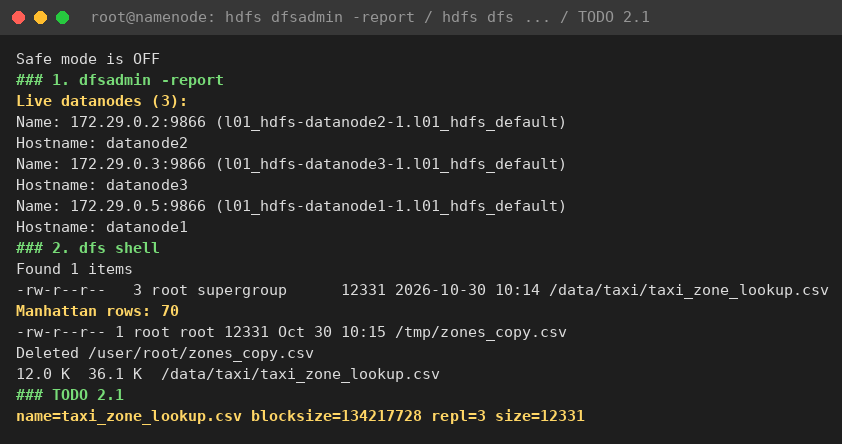
\includegraphics[keepaspectratio]{L01/img/01_cluster_and_dfs_shell.png}}
\pandocbounded{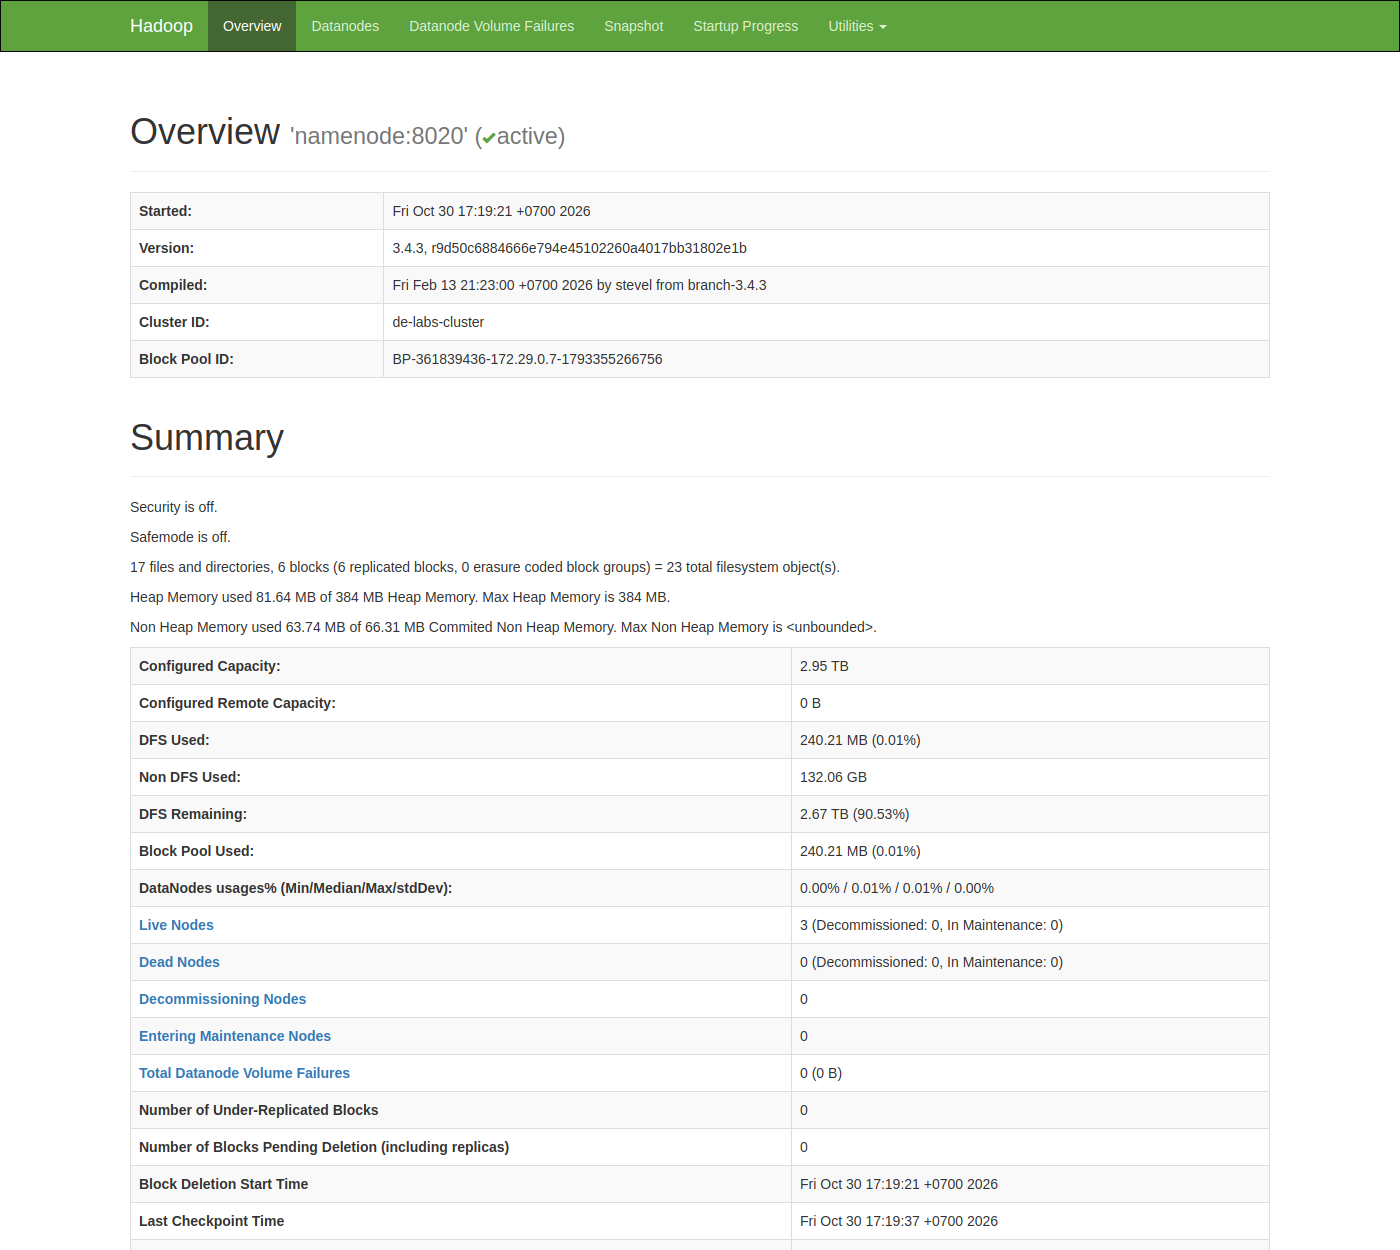
\includegraphics[keepaspectratio]{L01/img/11_ui_namenode_overview_healthy.png}}
\pandocbounded{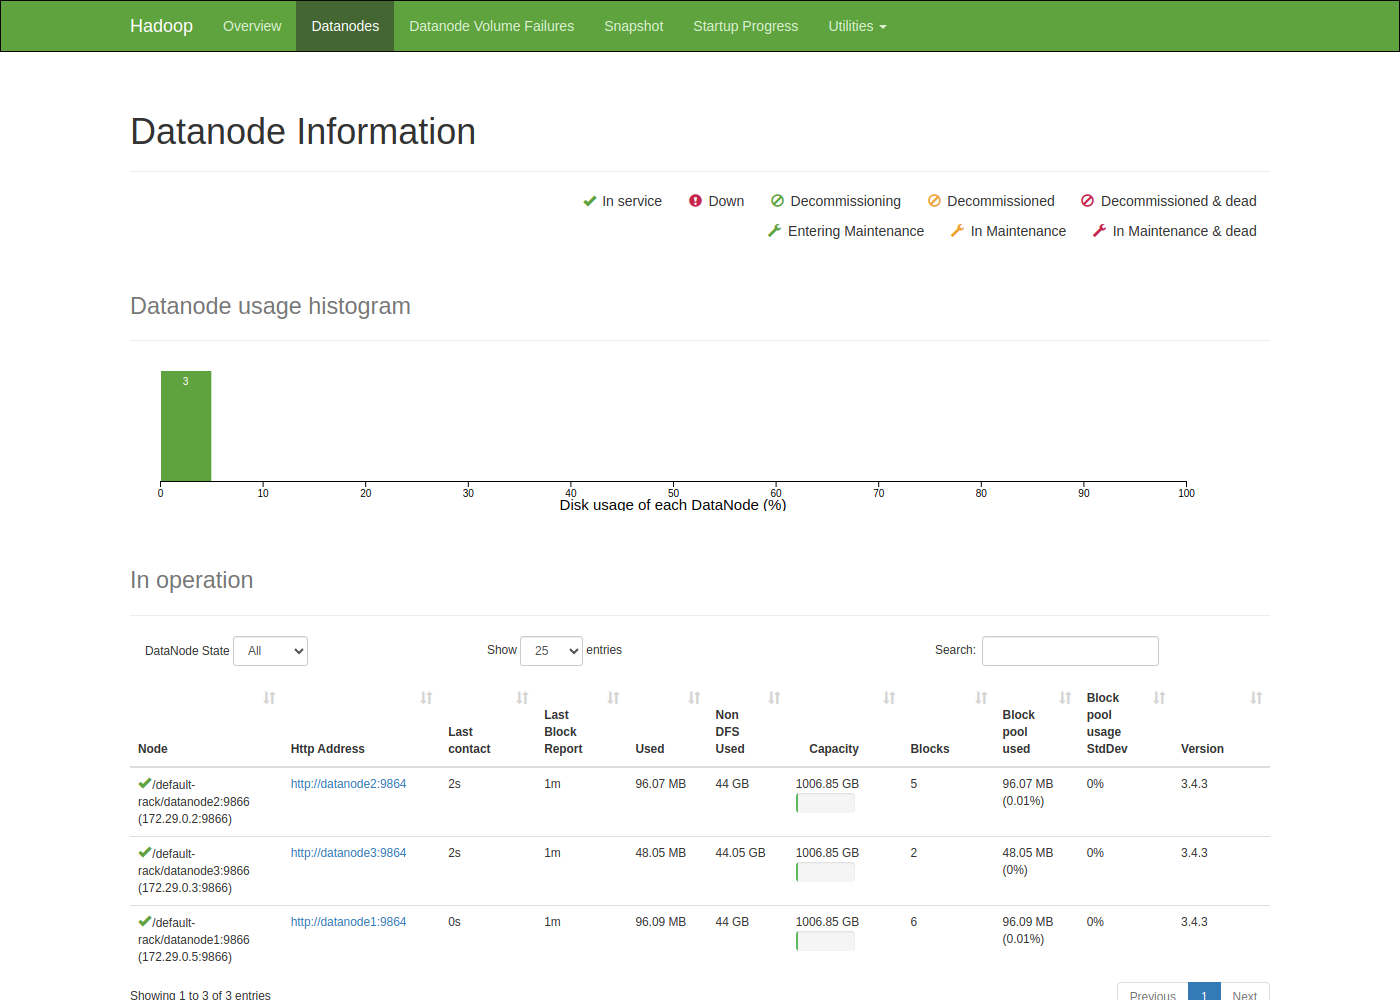
\includegraphics[keepaspectratio]{L01/img/12_ui_datanodes_healthy.png}}

\textbf{TODO 2.1}

\begin{Shaded}
\begin{Highlighting}[]
\ExtensionTok{hdfs}\NormalTok{ dfs }\AttributeTok{{-}stat} \StringTok{"name=\%n blocksize=\%o repl=\%r size=\%b"}\NormalTok{ /data/taxi/taxi\_zone\_lookup.csv}
\CommentTok{\# name=taxi\_zone\_lookup.csv blocksize=134217728 repl=3 size=12331}
\end{Highlighting}
\end{Shaded}

\subsection{3. Block mặc định (128 MB) và block 16
MB}\label{block-mux1eb7c-ux111ux1ecbnh-128-mb-vuxe0-block-16-mb}

\begin{longtable}[]{@{}lll@{}}
\toprule\noalign{}
Upload & Số block & Kích thước block \\
\midrule\noalign{}
\endhead
\bottomrule\noalign{}
\endlastfoot
mặc định 128 MB & 1 & 49,961,641 \\
\texttt{-D\ dfs.blocksize=16m} & 3 & 16,777,216 + 16,777,216 +
16,407,209 \\
\end{longtable}

\begin{figure}
\centering
\pandocbounded{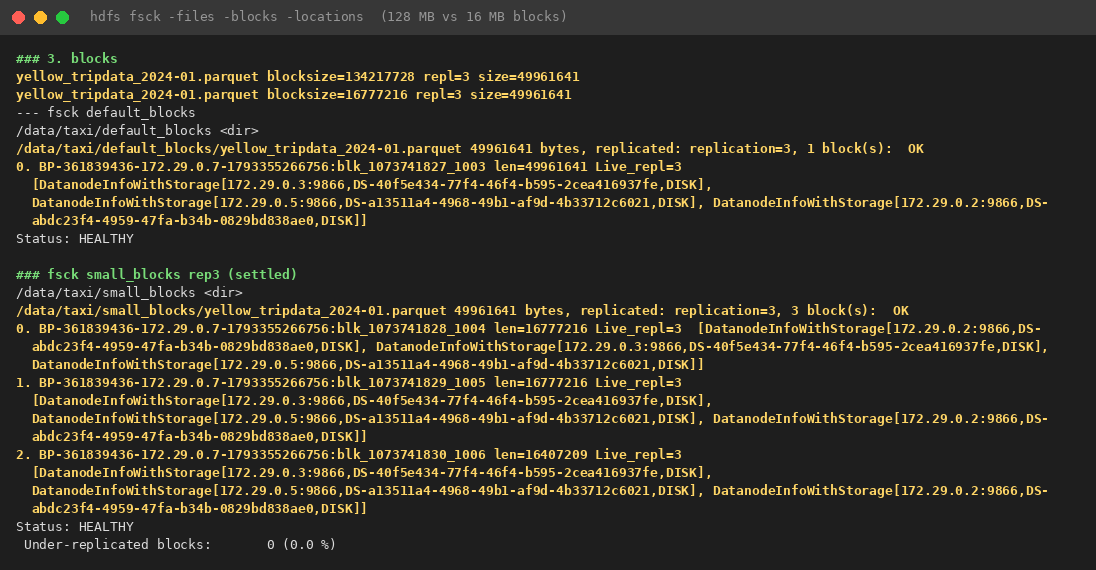
\includegraphics[keepaspectratio]{L01/img/02_blocks_128m_vs_16m.png}}
\caption{fsck 128m vs 16m}
\end{figure}

Các file block vật lý trên datanode1
(\texttt{blk\_\textless{}id\textgreater{}} +
\texttt{blk\_\textless{}id\textgreater{}\_\textless{}genstamp\textgreater{}.meta});
block cuối chỉ 16,407,209 byte, không bị pad lên 16 MB:

\begin{figure}
\centering
\pandocbounded{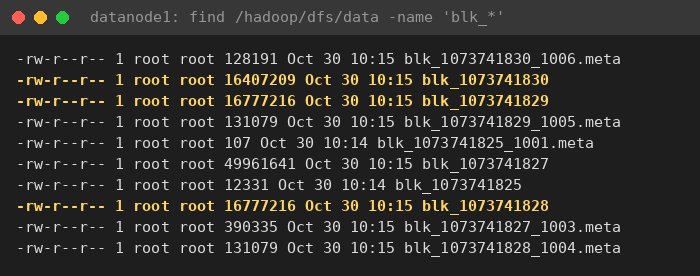
\includegraphics[keepaspectratio]{L01/img/03_physical_block_files_datanode1.png}}
\caption{block files}
\end{figure}

\subsection{4. Replication factor}\label{replication-factor}

\texttt{setrep\ -w\ 2} → \texttt{Live\_repl=2} cho cả 3 block; dung
lượng raw của \texttt{small\_blocks} giảm từ 142.9 M xuống \textbf{95.3
M}.

\textbf{TODO 4.1}

\begin{Shaded}
\begin{Highlighting}[]
\ExtensionTok{hdfs}\NormalTok{ dfs }\AttributeTok{{-}D}\NormalTok{ dfs.replication=1 }\AttributeTok{{-}put}\NormalTok{ /datasets/data/taxi/taxi\_zone\_lookup.csv /tmp/one\_replica.csv}
\CommentTok{\# one\_replica.csv repl=1   (replica duy nhất nằm trên 172.29.0.5 = datanode1)}
\end{Highlighting}
\end{Shaded}

\begin{figure}
\centering
\pandocbounded{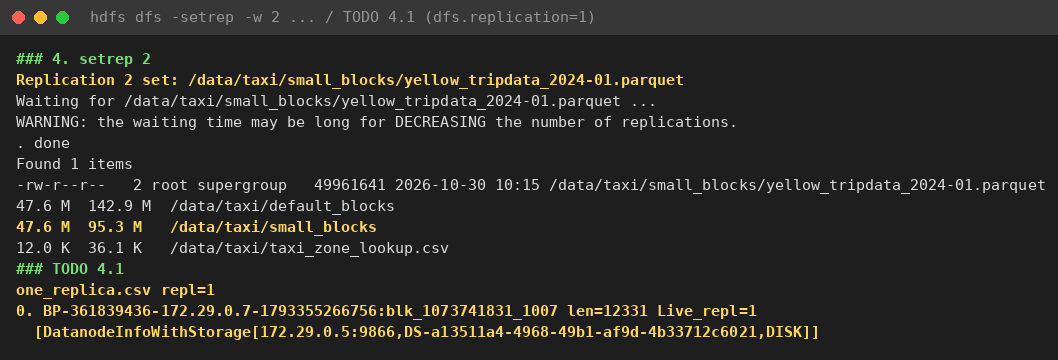
\includegraphics[keepaspectratio]{L01/img/04_setrep2_and_todo4.1.png}}
\caption{setrep}
\end{figure}

\subsection{5. Tắt DataNode → under-replication →
re-replication}\label{tux1eaft-datanode-under-replication-re-replication}

Tắt \textbf{datanode3} (đang giữ replica của cả 3 block của file
\texttt{small\_blocks}).

\textbf{(a) \texttt{fsck} của file block 16 MB TRƯỚC khi tắt} (replica
nằm trên \texttt{.5} datanode1 và \texttt{.3} datanode3):

\begin{figure}
\centering
\pandocbounded{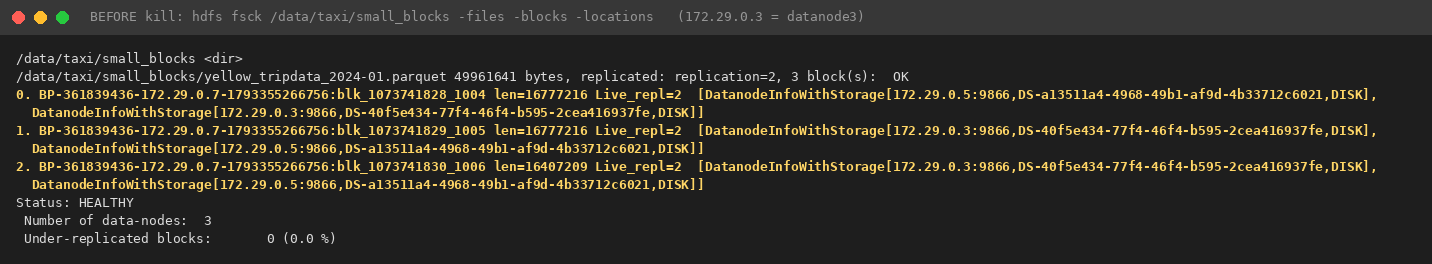
\includegraphics[keepaspectratio]{L01/img/05_fsck_small_blocks_BEFORE_kill.png}}
\caption{before}
\end{figure}

\textbf{(b) Thời gian đến khi node bị coi là chết:} \textbf{90 s}
(\texttt{Dead\ datanodes\ (1)} lúc t+90 s). Lúc t+94 s (10:17:40)
NameNode log
\texttt{removeDeadDatanode:\ lost\ heartbeat\ from\ 172.29.0.3}; từ lần
poll t+98 s trở đi \texttt{Under\ replicated\ blocks:\ 2}. Con số 90 s
khớp với lý thuyết 2 × recheck-interval (30 s) + 10 × heartbeat (3 s).

\pandocbounded{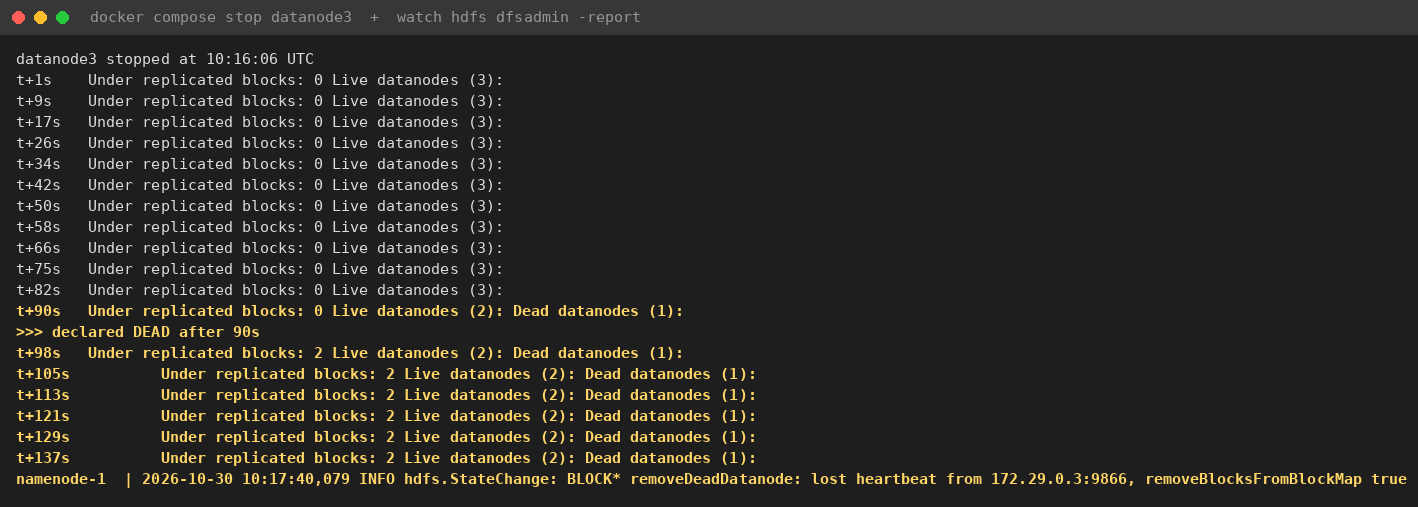
\includegraphics[keepaspectratio]{L01/img/06_kill_datanode3_timeline.png}}
\pandocbounded{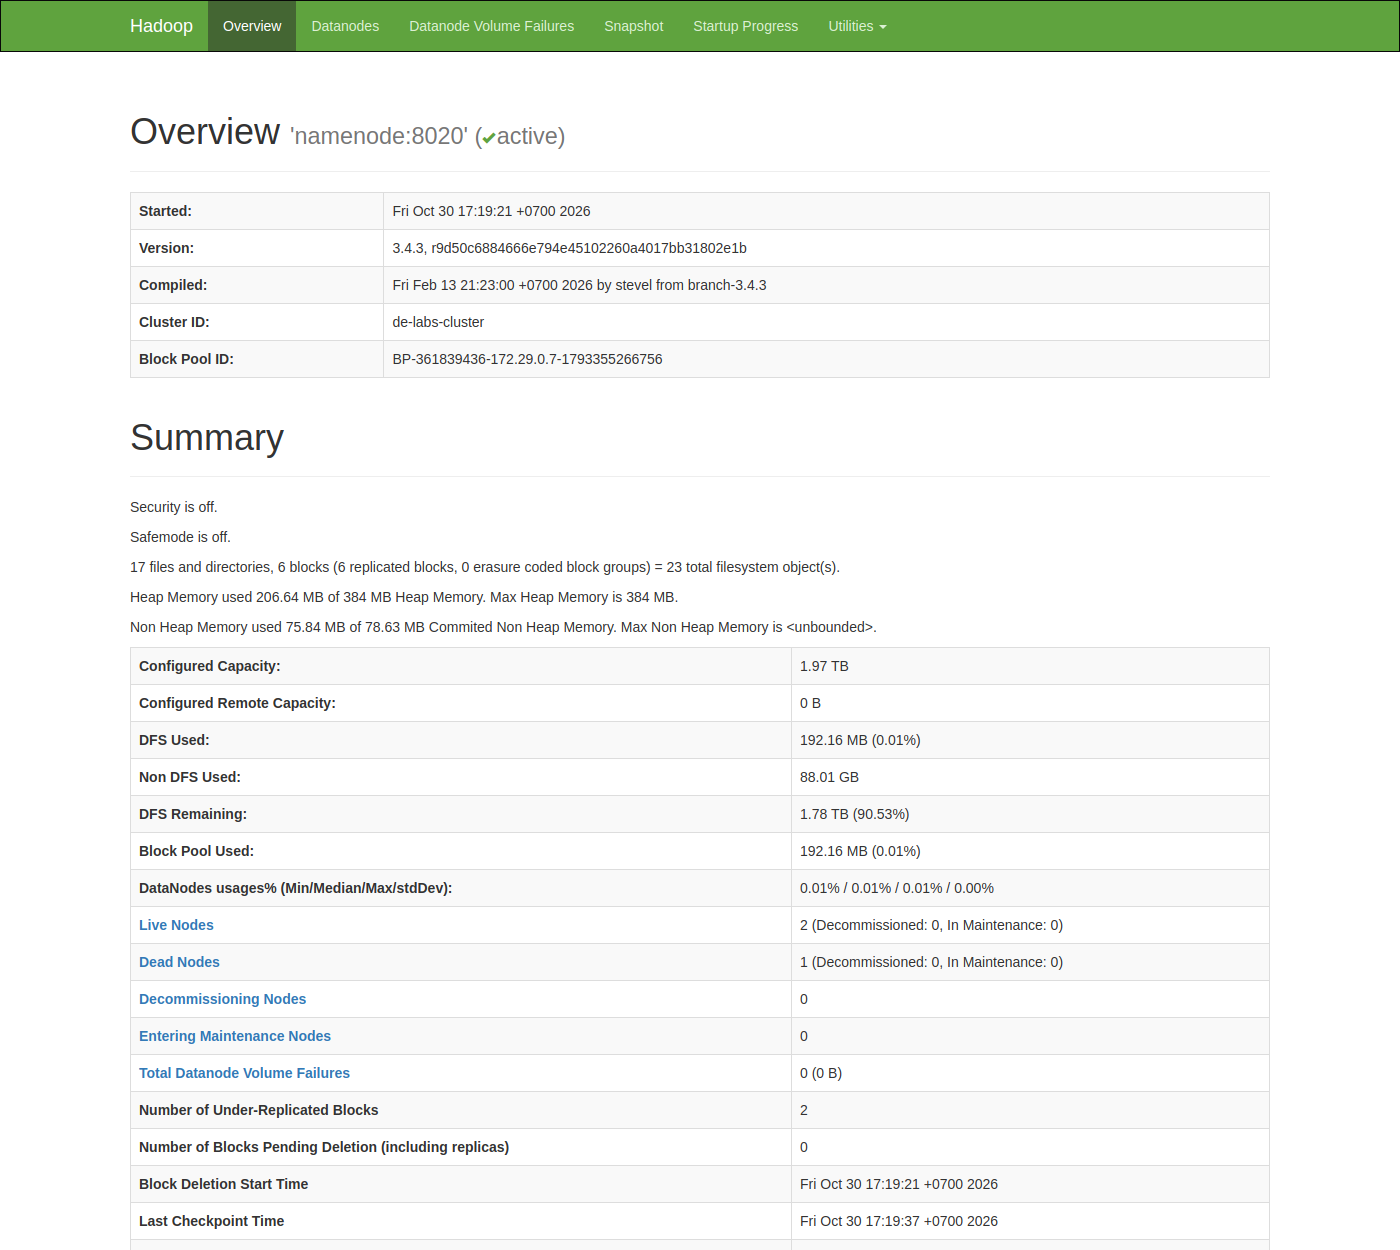
\includegraphics[keepaspectratio]{L01/img/14_ui_overview_datanode3_DEAD.png}}
\pandocbounded{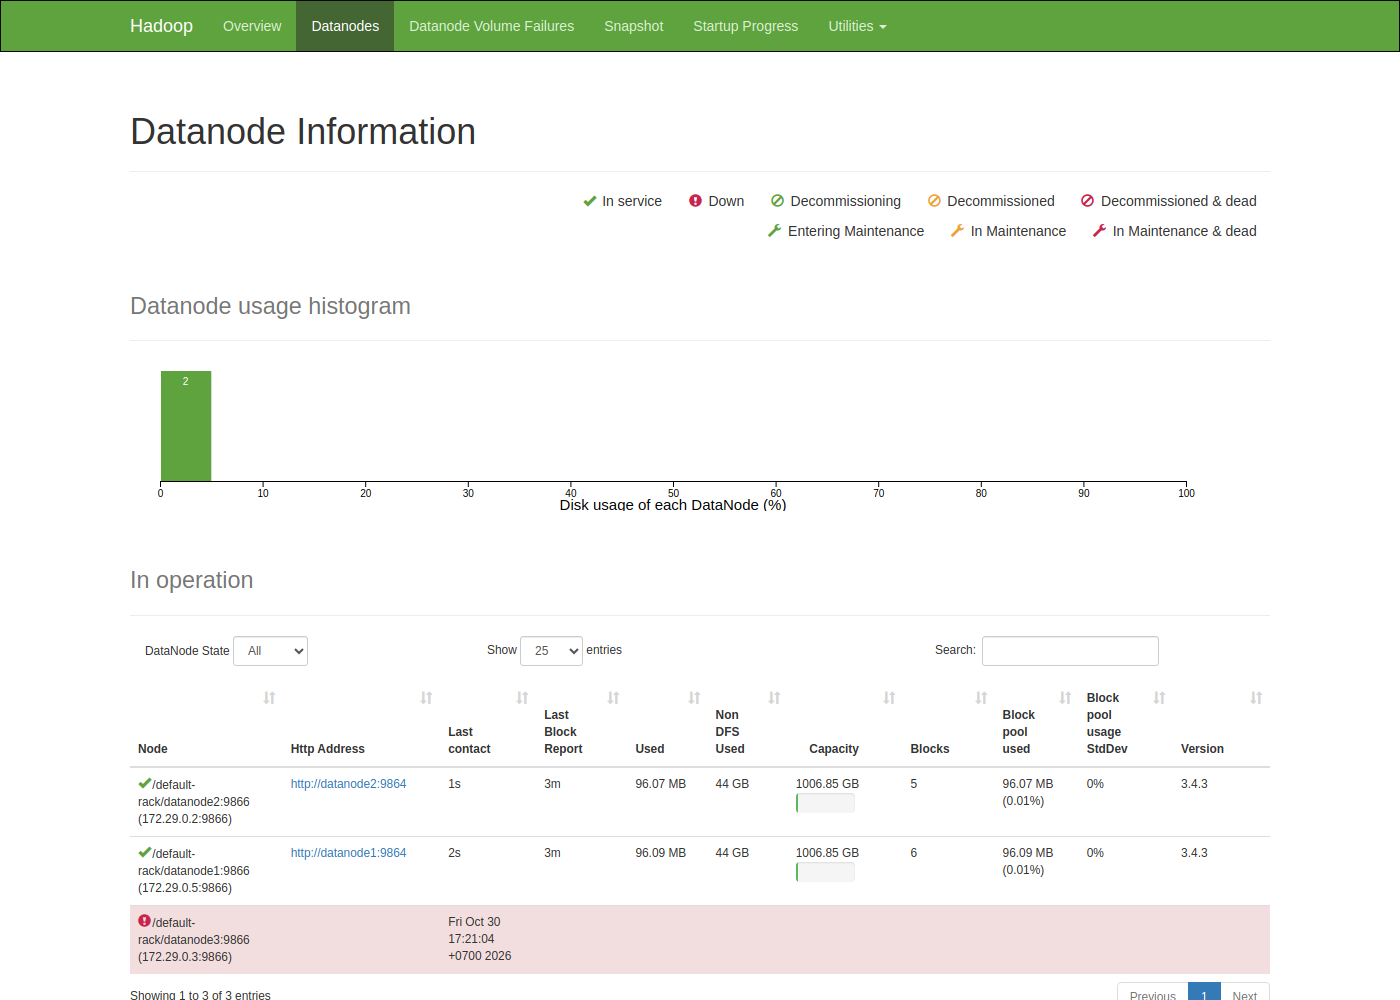
\includegraphics[keepaspectratio]{L01/img/15_ui_datanodes_datanode3_DEAD.png}}

\textbf{(c) \texttt{fsck} của file block 16 MB SAU khi tắt:} cả 3 block
vẫn \texttt{Live\_repl=2}, nhưng replica trên \texttt{.3} đã được
\textbf{chép lại sang \texttt{.2} (datanode2)} → file trở lại
\texttt{OK}.

\begin{figure}
\centering
\pandocbounded{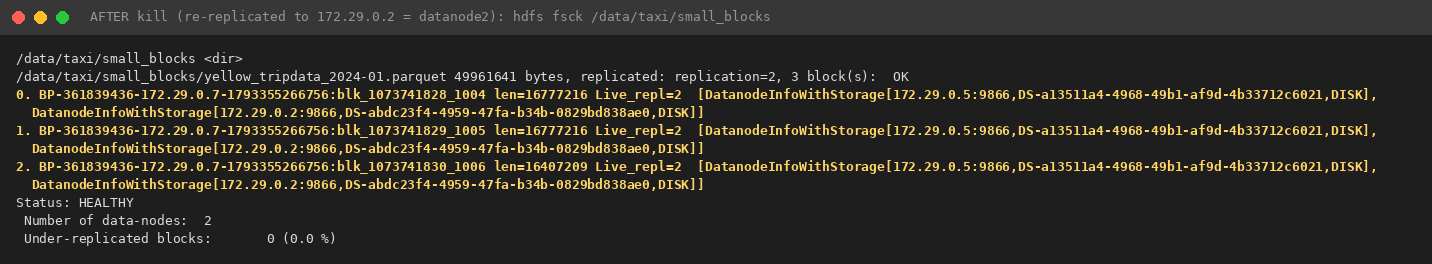
\includegraphics[keepaspectratio]{L01/img/07_fsck_small_blocks_AFTER_kill.png}}
\caption{after}
\end{figure}

Hai file replication 3 (\texttt{default\_blocks/...parquet},
\texttt{taxi\_zone\_lookup.csv}) vẫn \textbf{under-replicated} (2 block,
40 \%) nhưng \texttt{Status:\ HEALTHY}; md5 của file tải về trùng với
bản gốc → không mất dữ liệu. (\texttt{/tmp/one\_replica.csv} nằm trên
datanode1 nên không bị MISSING.)

\begin{figure}
\centering
\pandocbounded{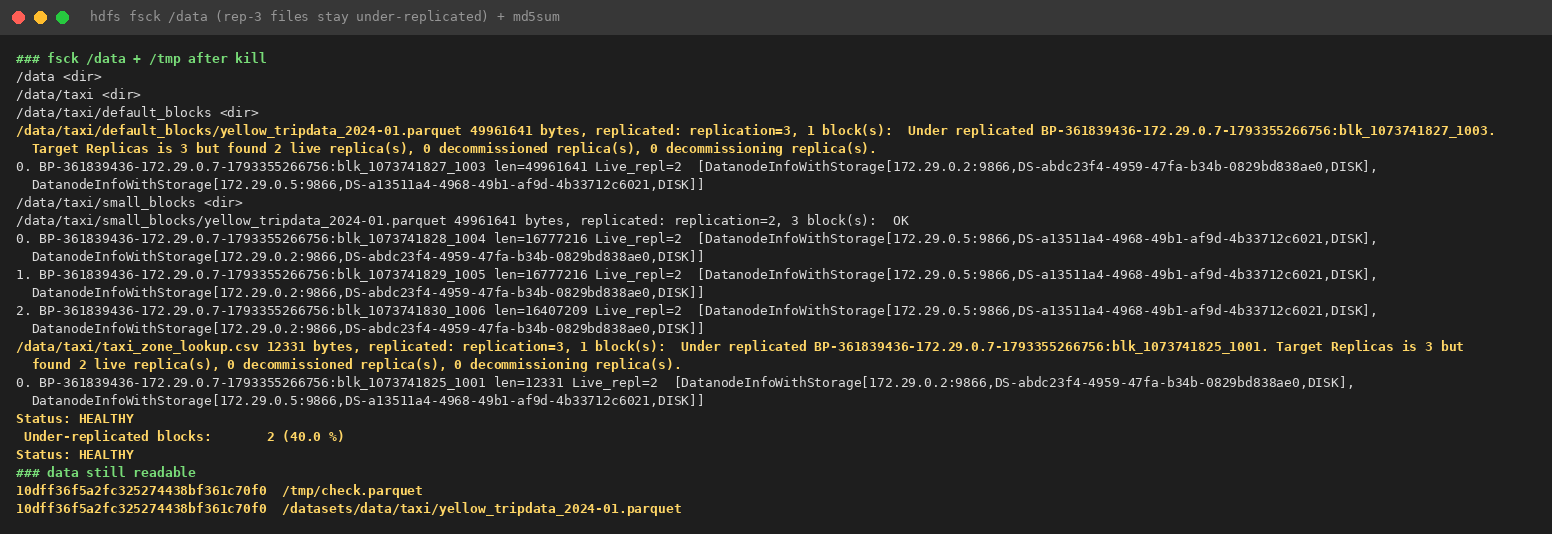
\includegraphics[keepaspectratio]{L01/img/08_fsck_data_underreplicated_md5.png}}
\caption{under-replicated + md5}
\end{figure}

Bật lại datanode3 → \texttt{Under-replicated\ 0},
\texttt{Over-replicated\ 0} (replica thừa đã bị xoá):

\begin{figure}
\centering
\pandocbounded{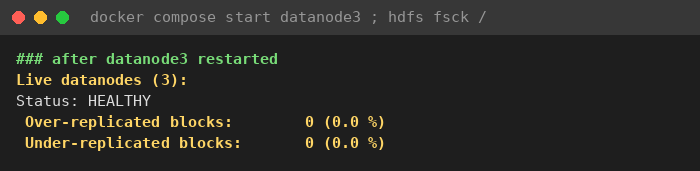
\includegraphics[keepaspectratio]{L01/img/09_datanode3_back.png}}
\caption{back}
\end{figure}

\subsection{6--7. Safe mode và fsimage}\label{safe-mode-vuxe0-fsimage}

\begin{figure}
\centering
\pandocbounded{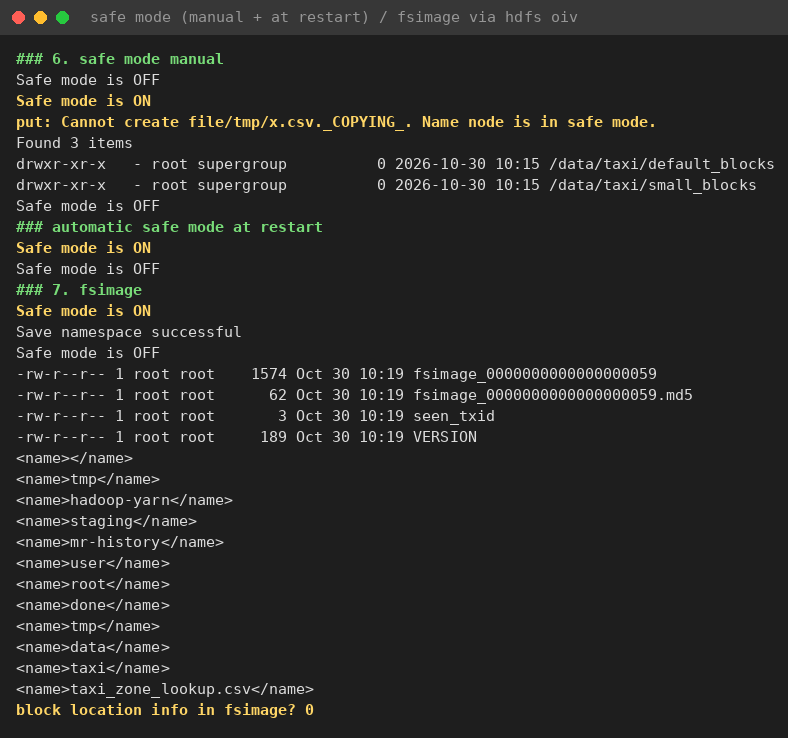
\includegraphics[keepaspectratio]{L01/img/10_safemode_fsimage.png}}
\caption{safemode}
\end{figure}

Trong safe mode lệnh ghi bị từ chối
(\texttt{Name\ node\ is\ in\ safe\ mode}), lệnh đọc vẫn chạy. Sau
\texttt{restart\ namenode} safe mode tự bật vài giây. fsimage
(\texttt{hdfs\ oiv}) chứa tên file/thư mục và block ID nhưng
\textbf{không có vị trí block} (grep thông tin DataNode/port 9866 trả về
0 dòng).

\subsection{Trả lời checkpoint}\label{trux1ea3-lux1eddi-checkpoint}

\textbf{Q1. File 300 MB, block mặc định, replication 3?} ⌈300/128⌉ =
\textbf{3 block} (128 + 128 + 44 MB) → \textbf{9 block replica} →
\textasciitilde{}\textbf{900 MB} đĩa raw (cộng thêm file \texttt{.meta}
checksum rất nhỏ). NameNode chỉ giữ 3 đối tượng block trong RAM, không
phụ thuộc replication.

\textbf{Q2. Vì sao block cuối nhỏ hơn 16 MB, có lãng phí 16 MB không?}
File kết thúc ở đó: 49,961,641 − 2 × 16,777,216 = 16,407,209 byte. Block
size chỉ là kích thước \textbf{tối đa}; file block trên DataNode đúng
bằng lượng dữ liệu thực (thấy rõ ở ảnh 03), nên không lãng phí đĩa.

\textbf{Q3. Danh sách vị trí block được lưu ở đâu? Restart NameNode thì
sao?} Chỉ nằm trong \textbf{RAM của NameNode}, không có trong fsimage
hay edit log (ảnh 10). Khi restart, NameNode dựng lại block map từ
\textbf{block report} của các DataNode, vì thế nó phải nằm trong safe
mode đến khi nhận đủ report.

\textbf{Q4. Vì sao file replication 2 được chữa còn file replication 3
thì không?} Re-replication cần một DataNode \textbf{chưa có} replica của
block đó. Khi chỉ còn 2 node sống: block rep-2 mất một bản trên
datanode3 → chép được sang datanode2 (node còn trống). Block rep-3 thì
đã có bản trên \textbf{cả hai} node còn lại, không còn node thứ ba để
đặt bản sao, và HDFS không bao giờ đặt 2 replica của cùng một block trên
một DataNode. Vì vậy nó vẫn under-replicated cho đến khi datanode3 quay
lại.

\textbf{Q5. \texttt{fsck} báo gì khi under-replicated, vì sao không phải
lỗi?} \texttt{Status:\ HEALTHY} kèm
\texttt{Under-replicated\ blocks:\ 2\ (40.0\ \%)}. HEALTHY nghĩa là
block nào cũng có ít nhất \texttt{dfs.namenode.replication.min} (=1)
replica sống, nên toàn bộ dữ liệu vẫn đọc được (md5 khớp).
Under-replication chỉ là \textbf{rủi ro} (giảm độ dư thừa); lỗi thật là
MISSING/CORRUPT.

\textbf{Q6. Với \texttt{recheck-interval} mặc định (5 phút) thì sao? Vì
sao timeout dài là mặc định tốt?} Node bị coi là chết sau 2 × 5 phút +
10 × 3 s = \textbf{10.5 phút} (lab: 90 s). Timeout dài tránh
\textbf{replication storm}: một node reboot hay chập mạng ngắn sẽ khiến
cluster chép hàng TB block, rồi các bản đó lại thành thừa khi node quay
lại sau một phút, tốn băng thông và I/O. Trong lúc chờ, client vẫn tránh
các node \emph{stale} (30 s không có heartbeat) khi đọc/ghi.

\textbf{Q7. Vì sao NameNode khởi động trong safe mode, vì sao phải chặn
ghi?} Lúc khởi động NameNode biết namespace (fsimage + edits) nhưng chưa
biết block nằm ở đâu. Trước khi ≥ 99.9 \% block được báo cáo, nó không
phân biệt được block ``bị mất'' với block ``chưa báo cáo''. Nếu cho phép
ghi/xoá hoặc bắt đầu re-replication thì nó sẽ quyết định sai, ví dụ lên
lịch chép hàng loạt các block chỉ đơn giản là chưa được báo cáo. Safe
mode = chỉ đọc cho tới khi block map đáng tin cậy.

\textbf{Q8. 1 file 1 KB và 1 triệu file 1 KB: vì sao trường hợp sau là
vấn đề?} Mỗi file, thư mục và block là một object trong heap NameNode
(\textasciitilde150 B). 1 triệu file nhỏ = ≥ 2 triệu object ≈ 300 MB
heap cho vỏn vẹn 1 GB dữ liệu, cộng thêm 1 triệu RPC và sau này 1 triệu
map task (mỗi file một split). Đây là \textbf{small files problem}. Cách
xử lý: gộp file, dùng định dạng container (Parquet/ORC, SequenceFile,
HAR).

\newpage

\section{L02 --- MapReduce với Hadoop Streaming
(Python)}\label{l02-mapreduce-vux1edbi-hadoop-streaming-python}

Cluster: dùng lại cluster L01 (1 NN, 3 DN, RM, NM, JobHistory). Log gốc
trong các file \texttt{0*.txt} và \texttt{*combiner.log}; ảnh ở
\texttt{img/}.

\subsection{File nộp}\label{file-nux1ed9p}

\begin{longtable}[]{@{}
  >{\raggedright\arraybackslash}p{(\linewidth - 2\tabcolsep) * \real{0.5000}}
  >{\raggedright\arraybackslash}p{(\linewidth - 2\tabcolsep) * \real{0.5000}}@{}}
\toprule\noalign{}
\begin{minipage}[b]{\linewidth}\raggedright
File
\end{minipage} & \begin{minipage}[b]{\linewidth}\raggedright
Nội dung
\end{minipage} \\
\midrule\noalign{}
\endhead
\bottomrule\noalign{}
\endlastfoot
\texttt{wc\_mapper.py}, \texttt{wc\_reducer.py} & TODO 1--3 (word
count) \\
\texttt{zones\_mapper.py} & TODO 4--6 (map-side join với
\texttt{taxi\_zone\_lookup.csv}, counter \texttt{BAD\_RECORDS}) \\
\texttt{stretch\_avg\_fare/} & Stretch: giá cước trung bình theo zone
với combiner đúng \texttt{(sum,\ count)} \\
\end{longtable}

\pandocbounded{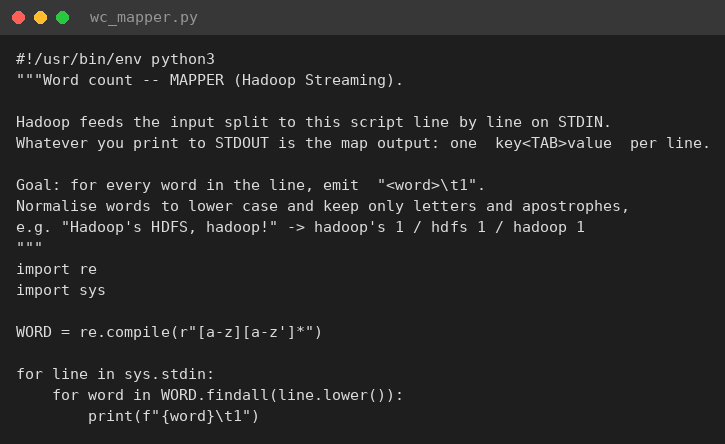
\includegraphics[keepaspectratio]{L02/img/code_wc_mapper.png}}
\pandocbounded{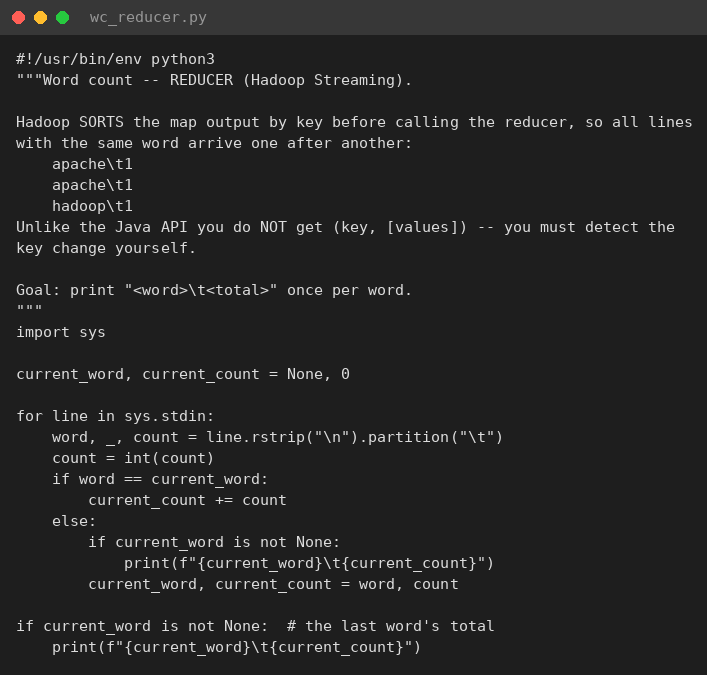
\includegraphics[keepaspectratio]{L02/img/code_wc_reducer.png}}
\pandocbounded{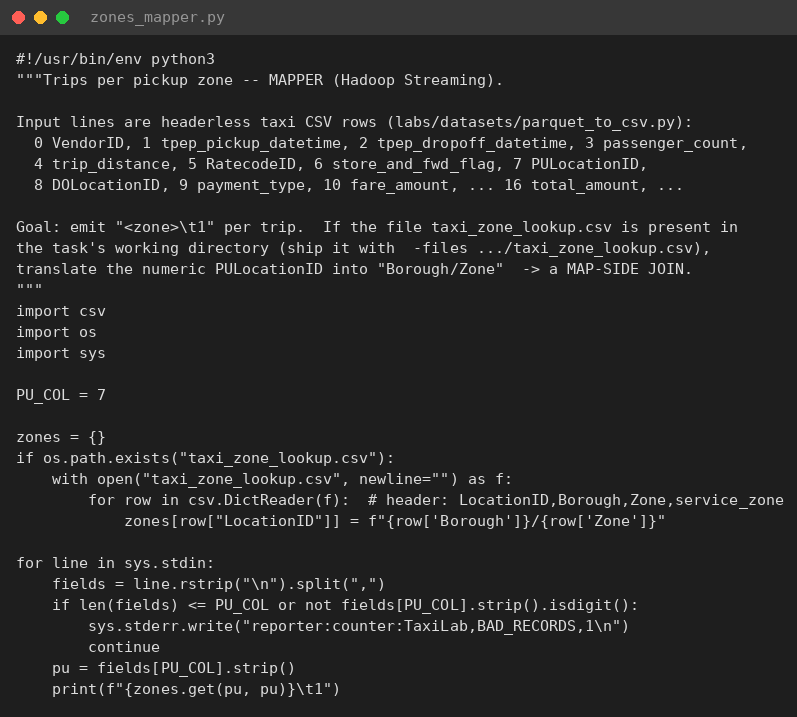
\includegraphics[keepaspectratio]{L02/img/code_zones_mapper.png}}

\subsection{1--2. Word count: test local và chạy trên
YARN}\label{word-count-test-local-vuxe0-chux1ea1y-truxean-yarn}

Test local
(\texttt{cat\ \textbar{}\ mapper\ \textbar{}\ sort\ \textbar{}\ reducer})
cho top 5
\texttt{the\ 25806,\ and\ 14340,\ of\ 14113,\ to\ 12103,\ a\ 9045}. Khi
\textbf{bỏ \texttt{sort}}, reducer in \texttt{the} ra \textbf{25,805
dòng} (mỗi lần xuất hiện gần như là một ``nhóm'' riêng) thay vì 1 dòng
tổng.

\begin{figure}
\centering
\pandocbounded{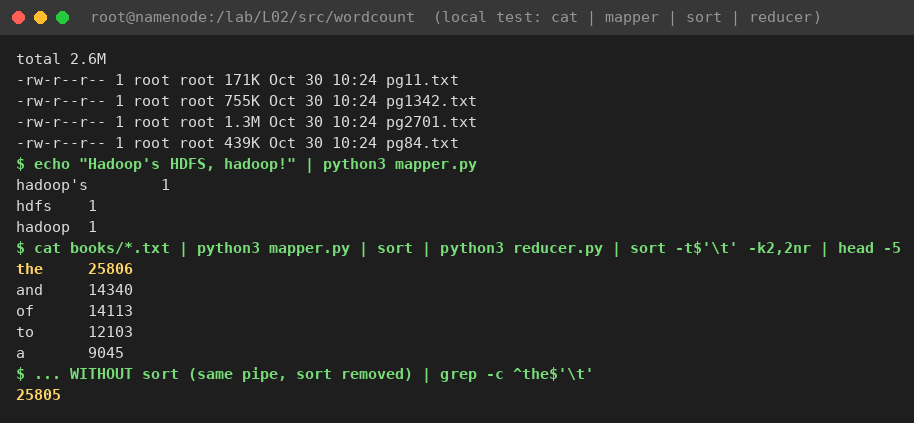
\includegraphics[keepaspectratio]{L02/img/01_wordcount_local_pipe.png}}
\caption{local pipe}
\end{figure}

Trên YARN: \texttt{Launched\ map\ tasks=4} (mỗi cuốn sách \textless{} 1
block là 1 split), \texttt{Reduce\ input\ groups=20967}; top 5 giống hệt
bản local.

\begin{figure}
\centering
\pandocbounded{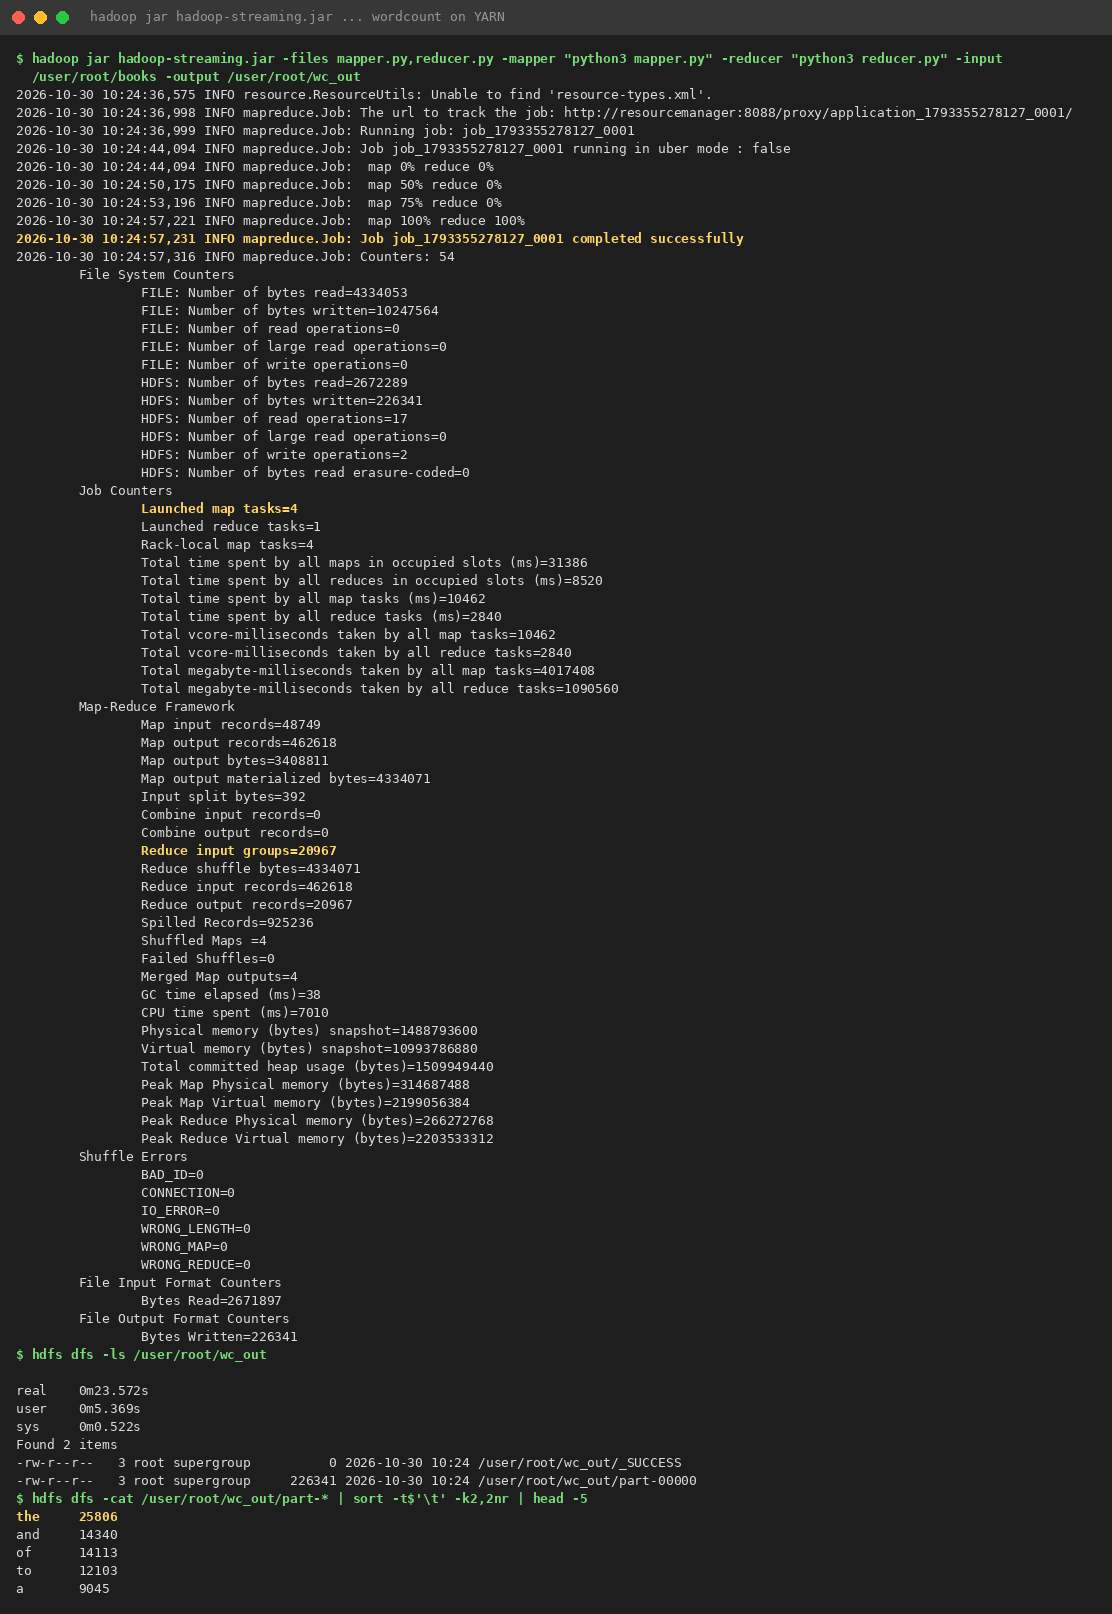
\includegraphics[keepaspectratio]{L02/img/02_wordcount_yarn_counters.png}}
\caption{wordcount yarn}
\end{figure}

\subsection{3--4. Dữ liệu taxi CSV và map-side
join}\label{dux1eef-liux1ec7u-taxi-csv-vuxe0-map-side-join}

1,000,000 dòng (92.8 MB) đưa lên HDFS với block 16 MB → \textbf{6 block
→ 6 map task}. Test local trên 1,000 dòng:
\texttt{Manhattan/East\ Village\ 59},
\texttt{Manhattan/Lincoln\ Square\ East\ 55}. Dòng hỏng được đếm qua
stderr \texttt{reporter:counter:TaxiLab,BAD\_RECORDS,1} (dữ liệu thật có
0 dòng hỏng nên counter không xuất hiện trong job).

\begin{figure}
\centering
\pandocbounded{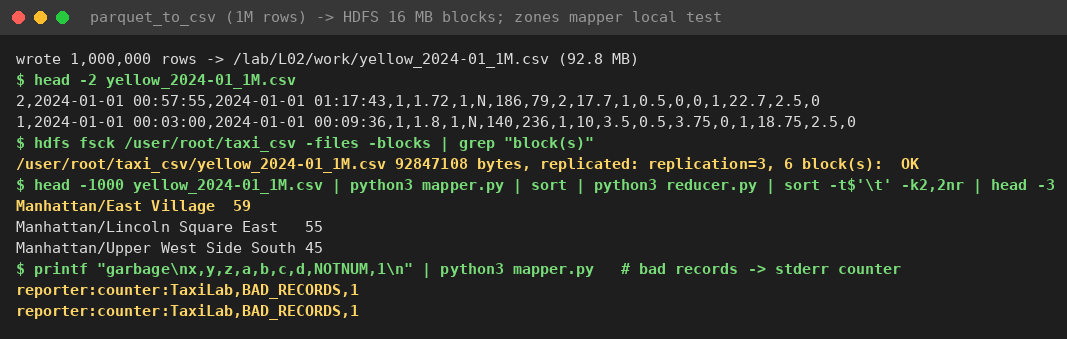
\includegraphics[keepaspectratio]{L02/img/03_taxi_csv_and_zones_local.png}}
\caption{taxi csv}
\end{figure}

\subsection{5. Combiner và không
combiner}\label{combiner-vuxe0-khuxf4ng-combiner}

\begin{longtable}[]{@{}lll@{}}
\toprule\noalign{}
Counter & Không combiner & Có combiner \\
\midrule\noalign{}
\endhead
\bottomrule\noalign{}
\endlastfoot
Launched map tasks & 6 & 6 \\
Map output records & 1,000,000 & 1,000,000 \\
Combine output records & 0 & 1,382 \\
Map output materialized bytes & 31,039,071 & 41,169 \\
Reduce shuffle bytes & 31,039,071 & 41,169 \\
Reduce input records & 1,000,000 & 1,382 \\
Wall-clock time & 30.3 s & 33.3 s \\
\end{longtable}

Kết quả hai lần chạy \textbf{giống hệt} (\texttt{diff} rỗng). Top zone:
\texttt{Queens/JFK\ Airport\ 59777},
\texttt{Manhattan/Midtown\ Center\ 48750}.

\begin{figure}
\centering
\pandocbounded{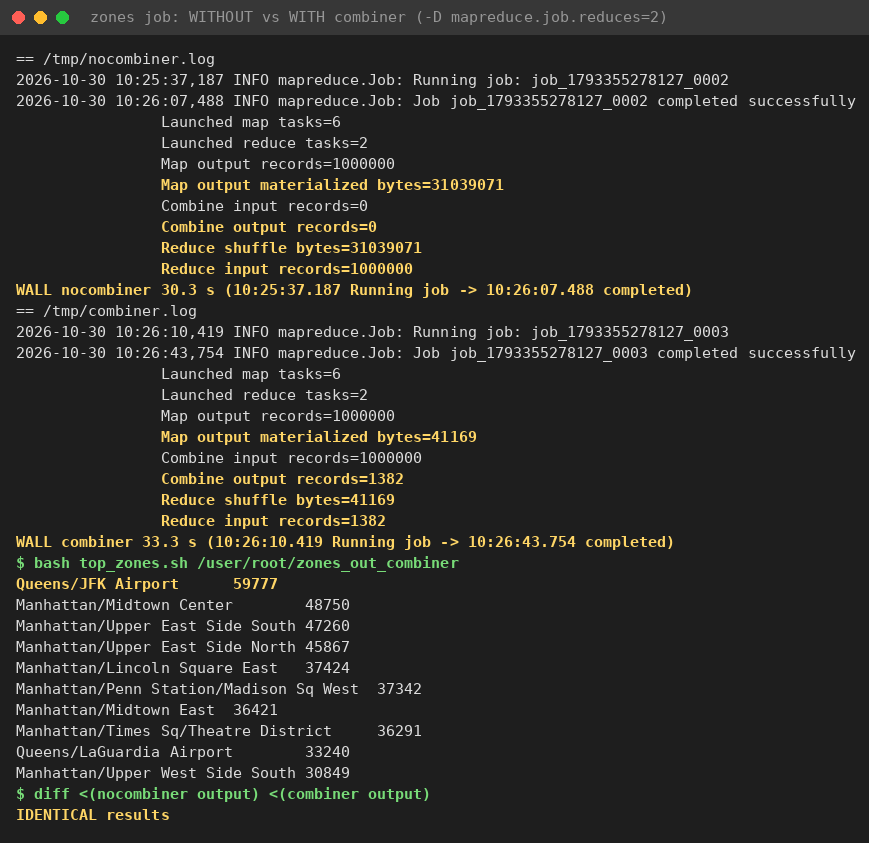
\includegraphics[keepaspectratio]{L02/img/04_combiner_vs_nocombiner_counters.png}}
\caption{combiner table}
\end{figure}

\subsection{6. YARN và JobHistory UI}\label{yarn-vuxe0-jobhistory-ui}

\pandocbounded{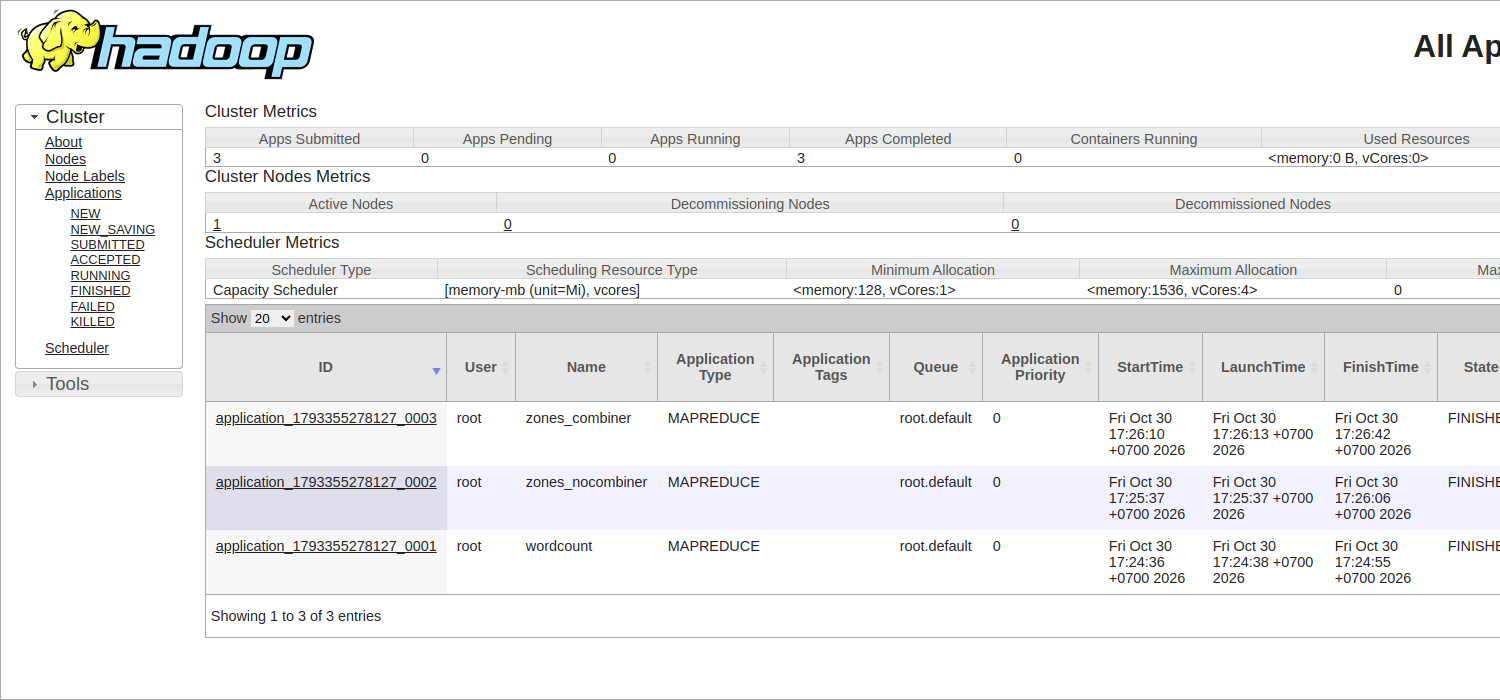
\includegraphics[keepaspectratio]{L02/img/10_ui_yarn_applications.png}}
\pandocbounded{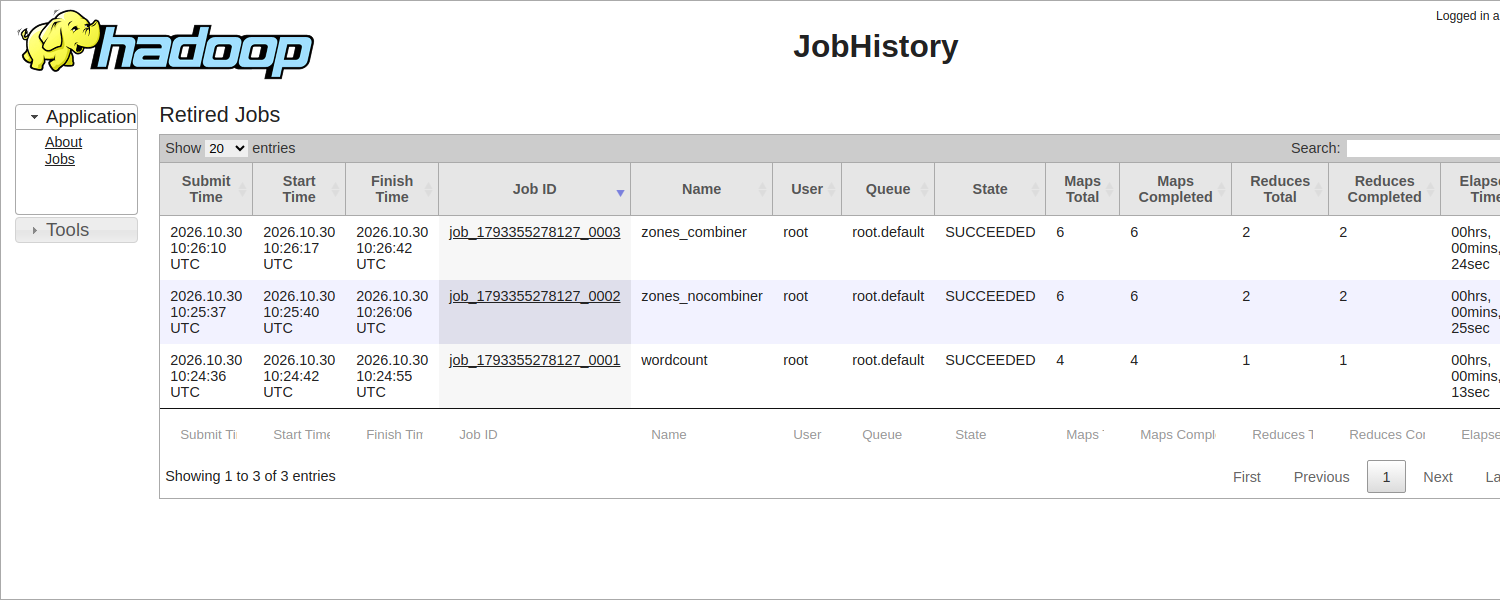
\includegraphics[keepaspectratio]{L02/img/11_ui_jobhistory_jobs.png}}
\pandocbounded{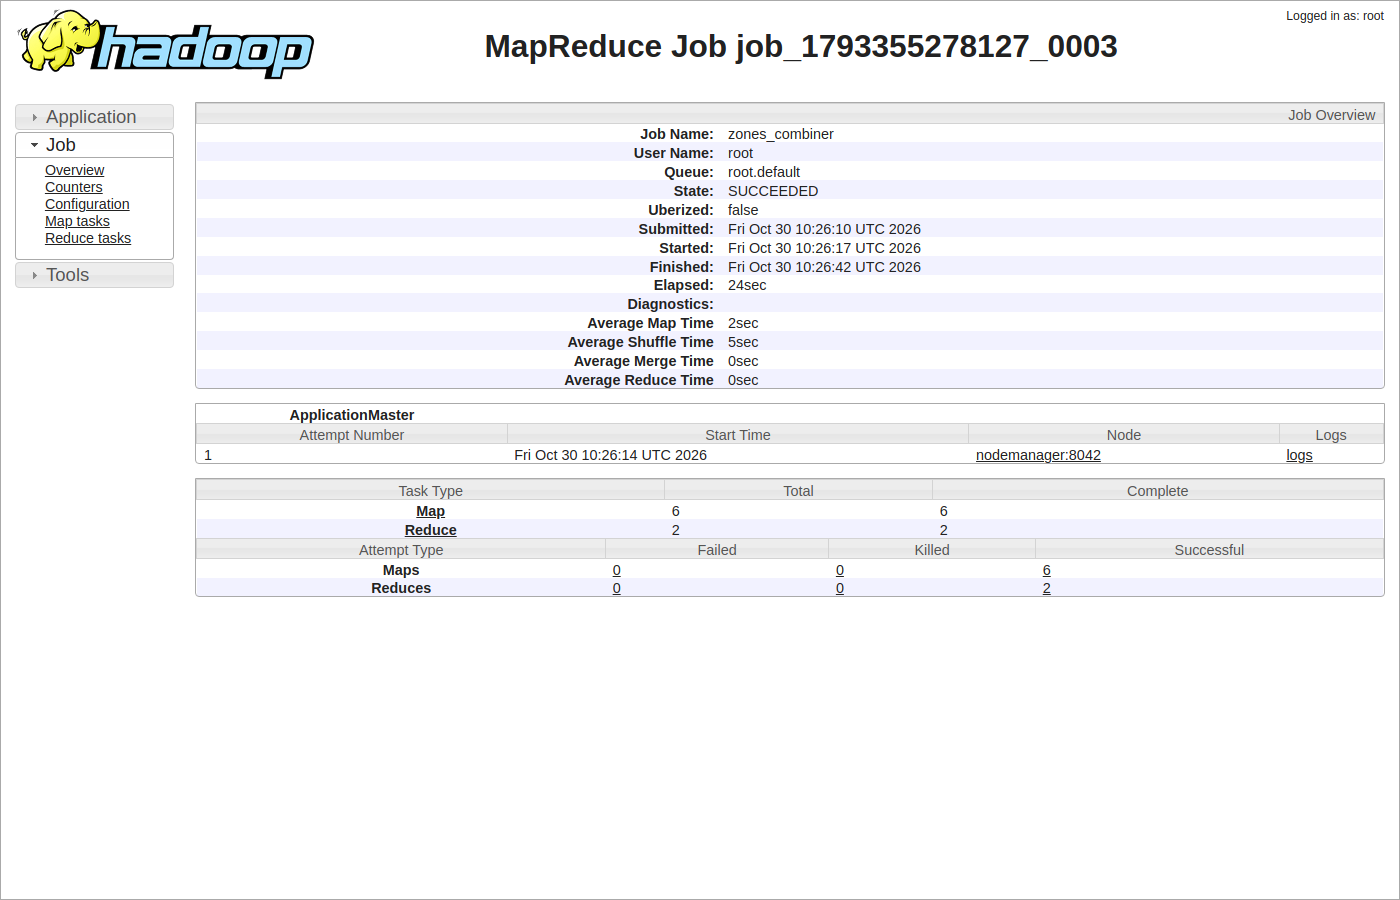
\includegraphics[keepaspectratio]{L02/img/14_ui_job_combiner_overview.png}}
\pandocbounded{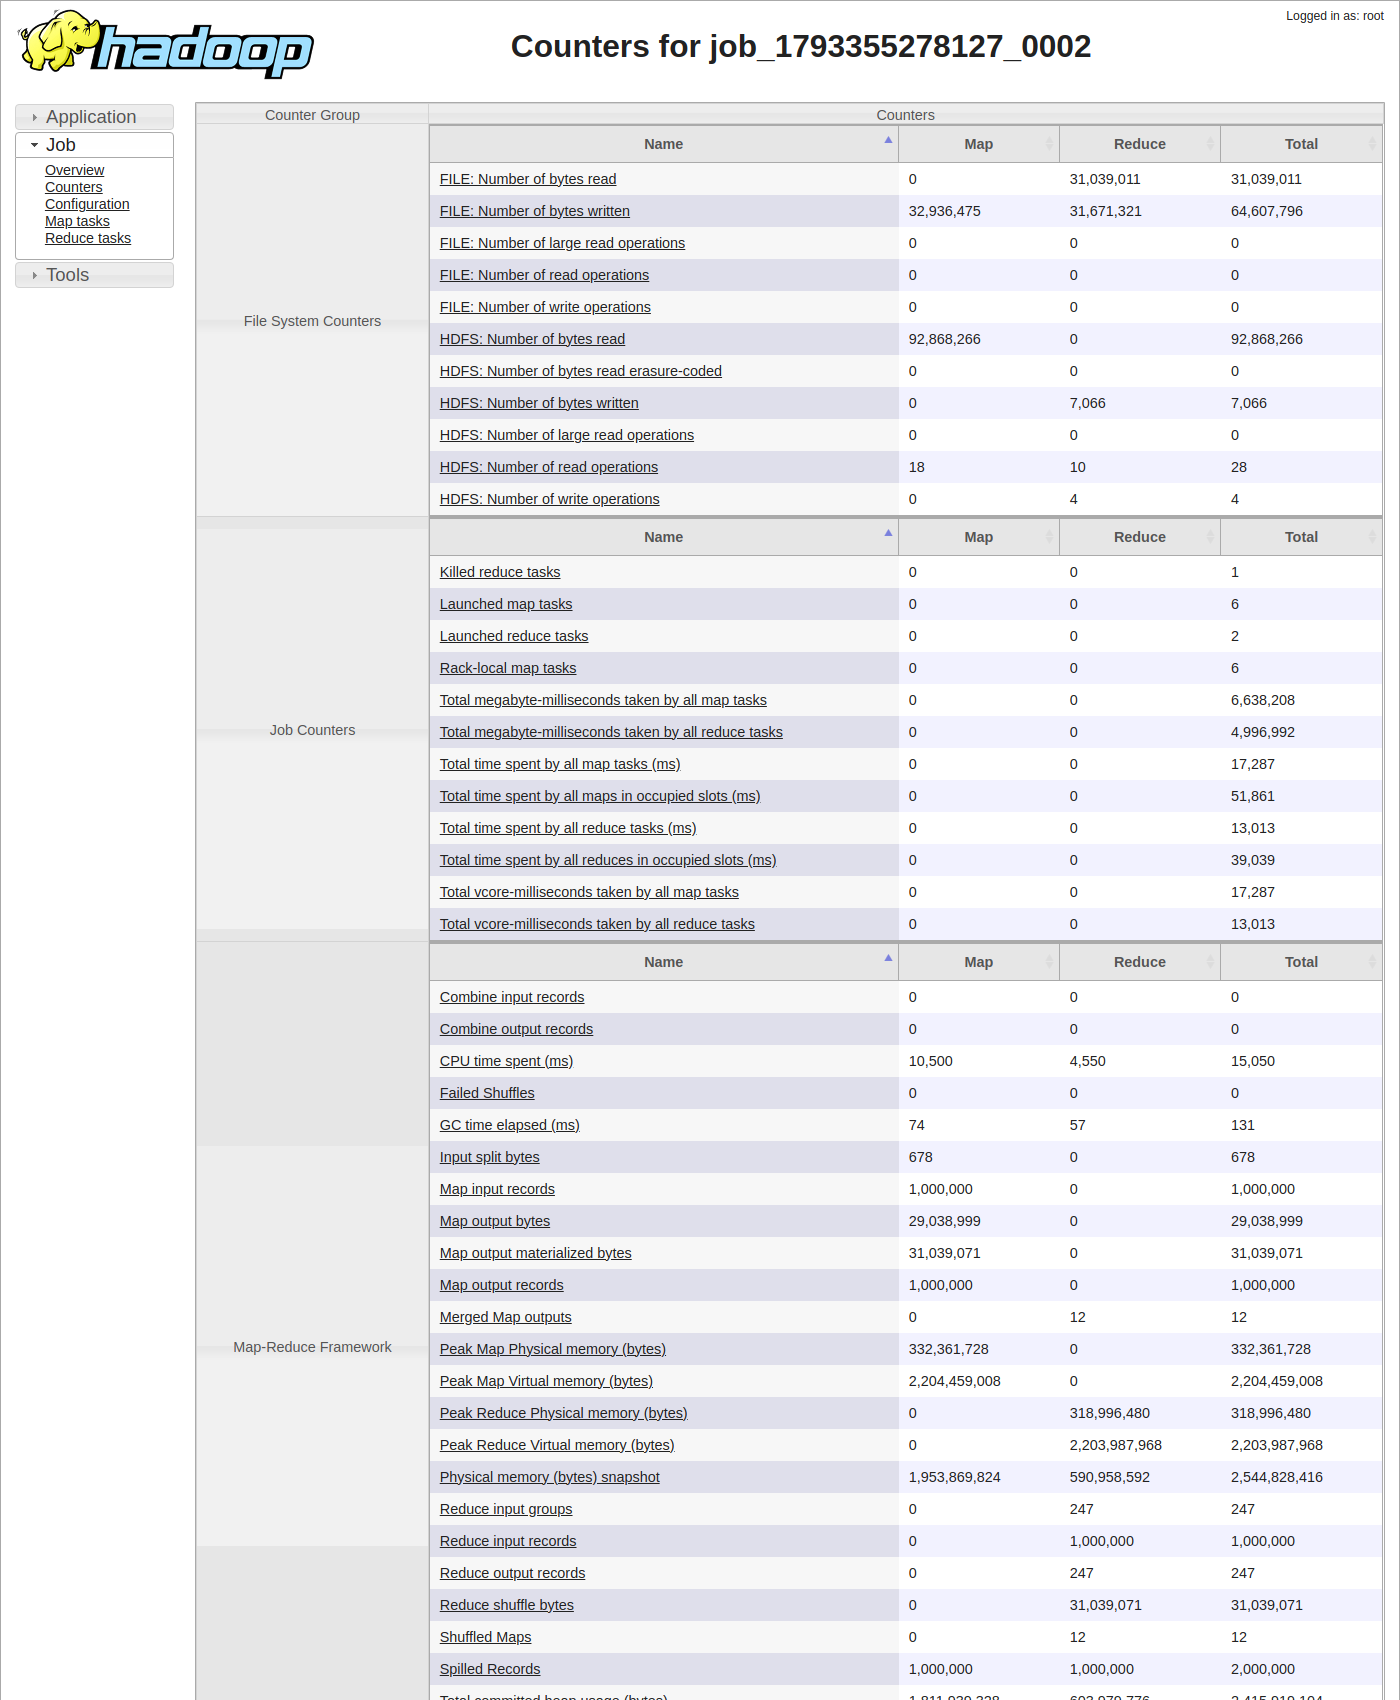
\includegraphics[keepaspectratio]{L02/img/12_ui_counters_nocombiner.png}}
\pandocbounded{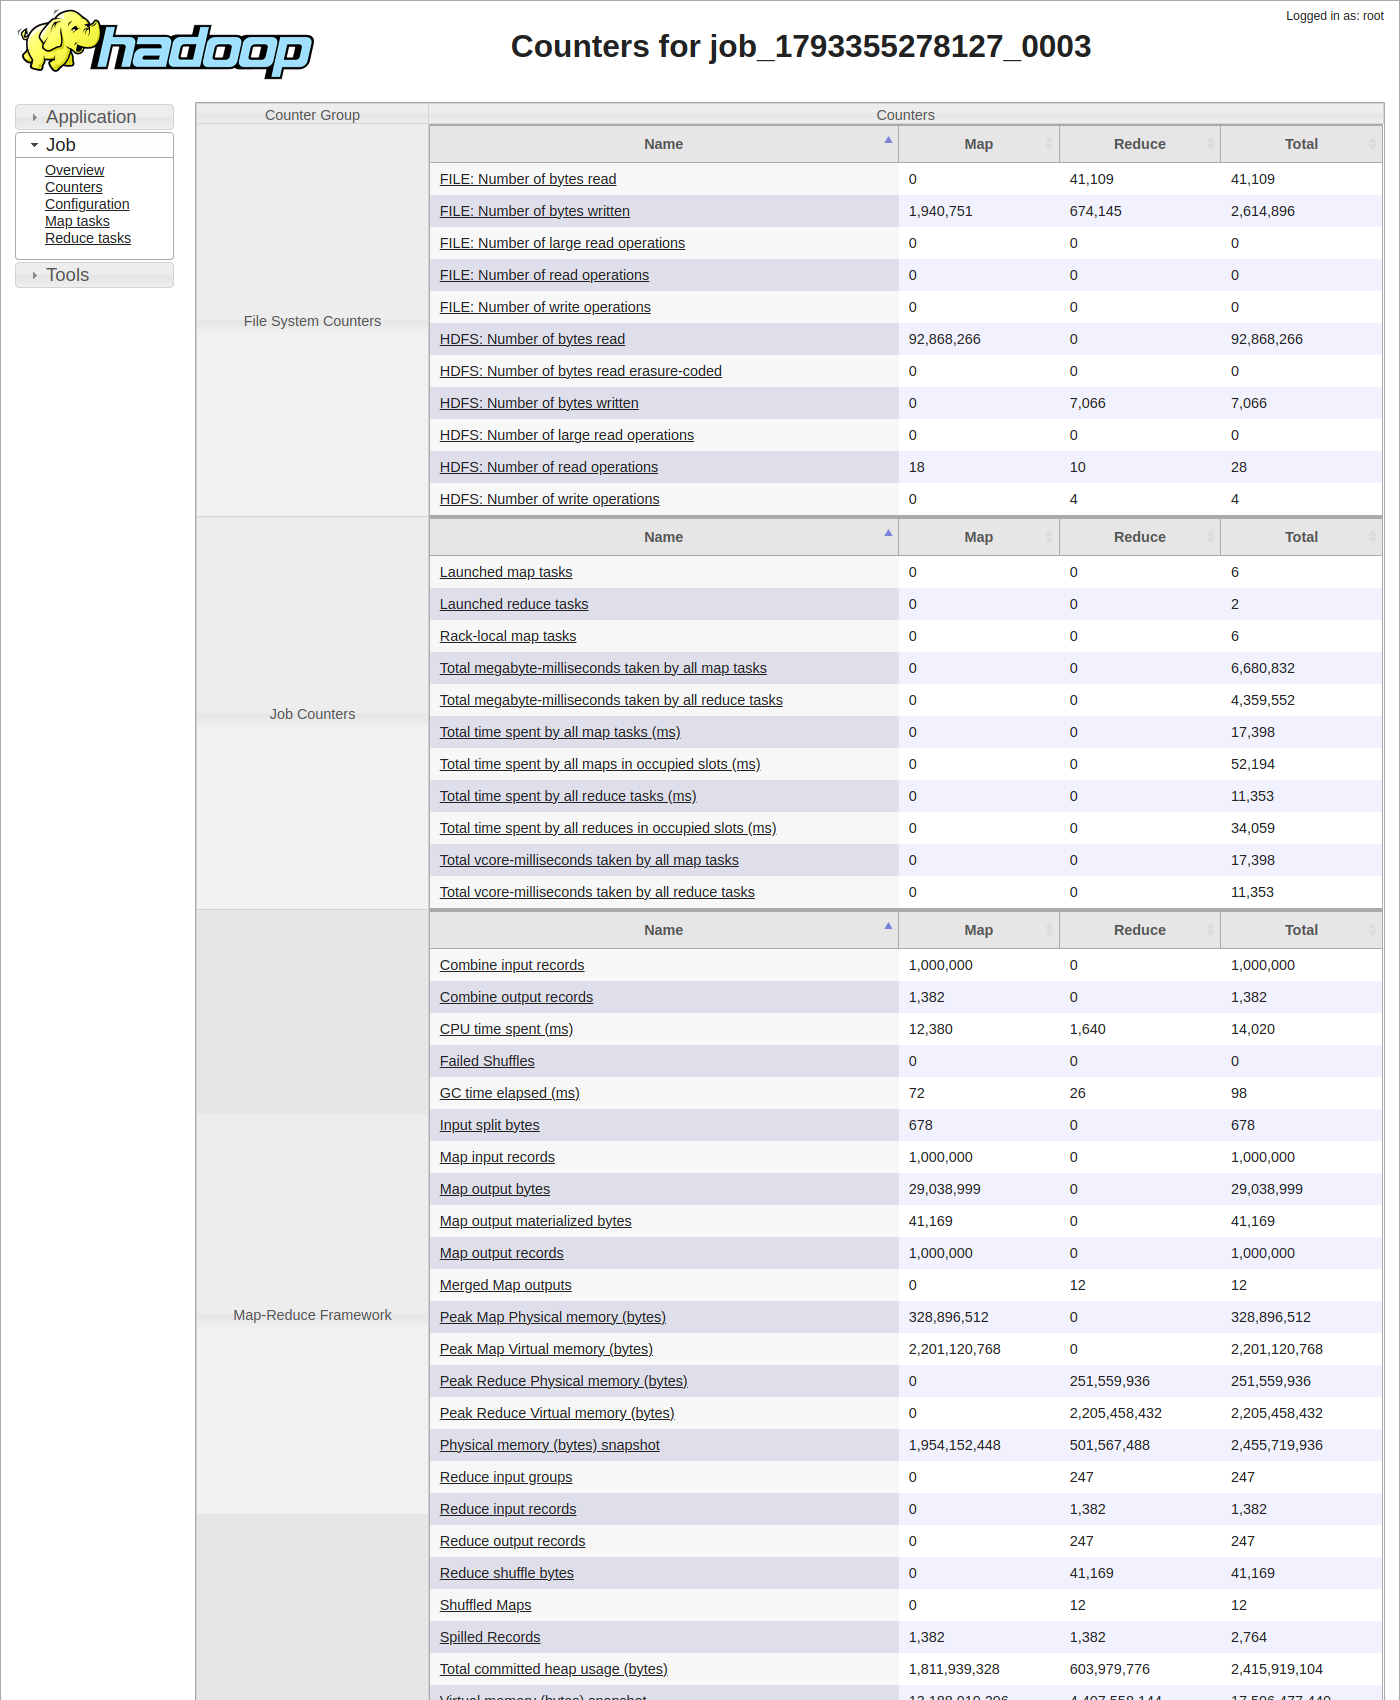
\includegraphics[keepaspectratio]{L02/img/13_ui_counters_combiner.png}}
\pandocbounded{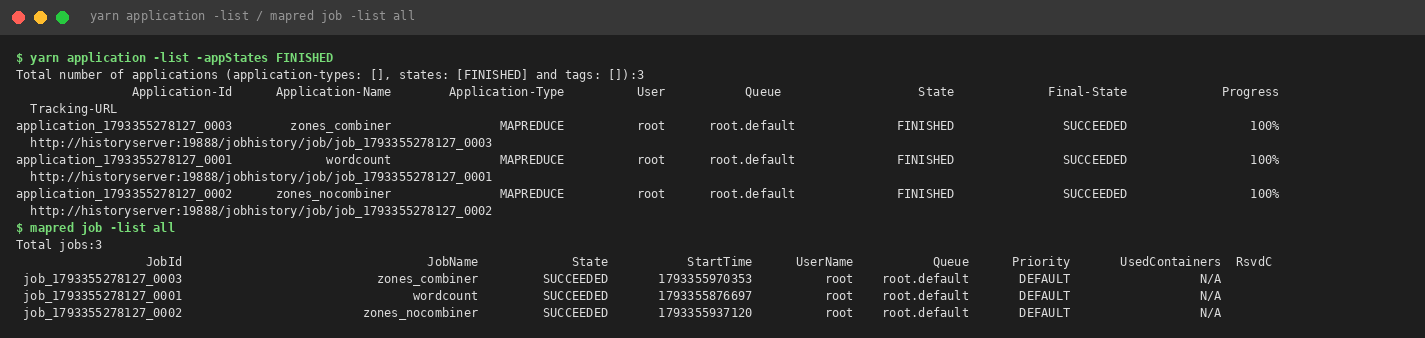
\includegraphics[keepaspectratio]{L02/img/05_yarn_cli.png}}

\subsection{Stretch (bonus): giá cước trung bình theo zone với combiner
đúng}\label{stretch-bonus-giuxe1-cux1b0ux1edbc-trung-buxecnh-theo-zone-vux1edbi-combiner-ux111uxfang}

Mapper emit \texttt{zone\ \textbackslash{}t\ fare,1}; combiner cộng dồn
\texttt{(sum,\ count)} và xuất \textbf{cùng định dạng} với input;
reducer cộng tiếp rồi mới chia \texttt{sum/count}. Kết quả JFK
\texttt{59.71} trên \texttt{59,777} chuyến, trùng với bản chạy local
không combiner, nghĩa là combiner không làm sai kết quả. Shuffle chỉ còn
56,289 byte.

\pandocbounded{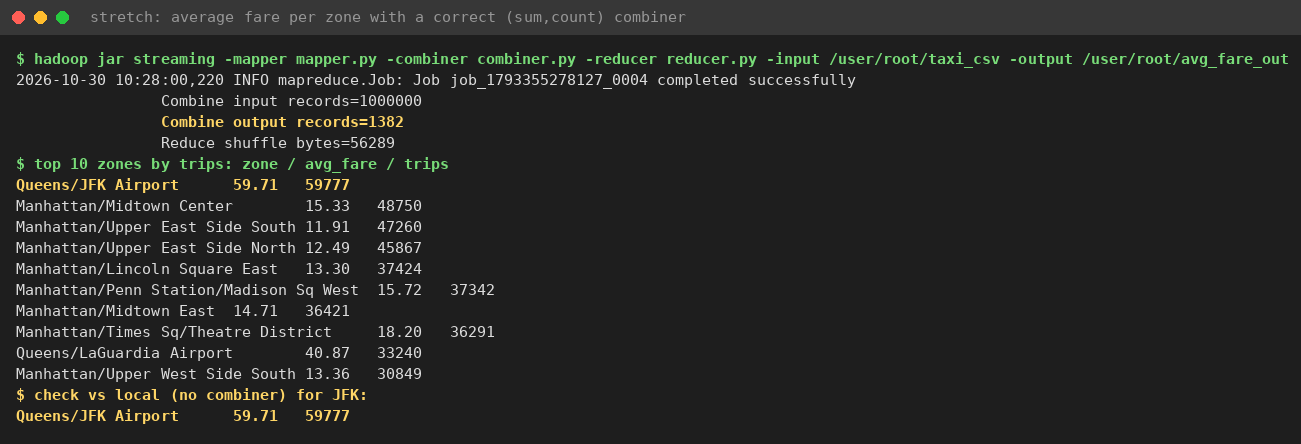
\includegraphics[keepaspectratio]{L02/img/06_stretch_avg_fare.png}}
\pandocbounded{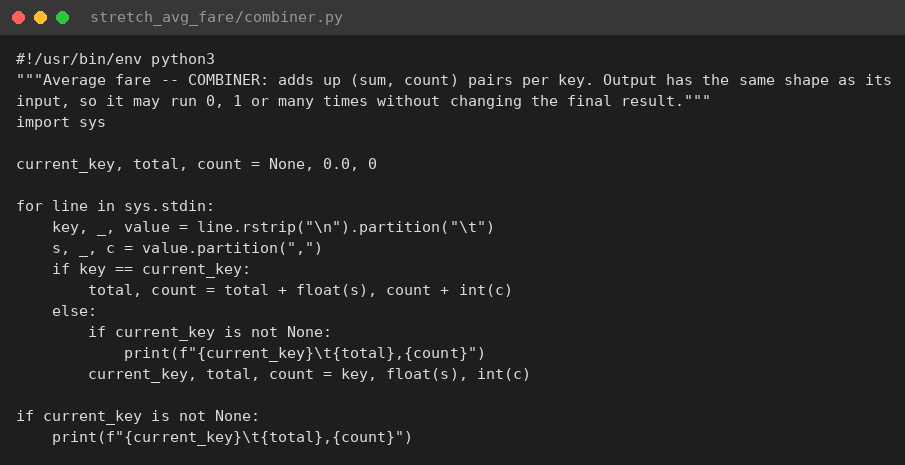
\includegraphics[keepaspectratio]{L02/img/code_stretch_avg_fare_combiner.png}}

\subsection{Trả lời checkpoint}\label{trux1ea3-lux1eddi-checkpoint-1}

\textbf{Q1.} Lệnh \texttt{sort} đóng vai trò \textbf{shuffle \& sort}:
nó gom các key giống nhau nằm liền nhau. Thiếu nó, reducer thấy cùng một
từ ở nhiều đoạn không liền nhau nên in ra nhiều lần với số đếm cục bộ
(thực nghiệm: \texttt{the} bị in 25,805 lần).

\textbf{Q2.} Streaming chỉ đưa cho reducer một \textbf{luồng dòng đã
sort}; khái niệm ``nhóm''
\texttt{(key,\ Iterable\textless{}values\textgreater{})} nằm trong
framework Java. Reducer Python phải tự phát hiện ranh giới key
(\texttt{current\_key}) và nhớ in key cuối cùng.

\textbf{Q3.} \textbf{6 map task} = 6 input split = 6 block HDFS 16 MB
của file CSV 92.8 MB (mặc định mỗi block là một split). Wordcount có 4
map vì mỗi cuốn sách nhỏ hơn 1 block nên là 1 split. \textbf{2 reduce
task} vì đặt \texttt{-D\ mapreduce.job.reduces=2} (mặc định là 1): số
reducer do người dùng chọn, không suy ra từ dữ liệu.

\textbf{Q4.} Shuffle giảm \textbf{\textasciitilde754 lần} (31,039,071 →
41,169 byte). Mỗi map task chỉ xuất một bản ghi cho mỗi \textbf{zone
khác nhau mà nó gặp} (\textasciitilde230--260 zone) × 6 map ≈ 1,382. Chỉ
các tổng cục bộ này đi qua mạng.

\textbf{Q5.} Combiner không nhanh hơn (33.3 s so với 30.3 s) vì trên một
máy, shuffle chỉ là copy qua đĩa/loopback, gần như miễn phí, trong khi
combiner thêm một process Python phải đọc, parse và sort lại 1 triệu bản
ghi ở mỗi map. Trên cluster thật, shuffle đi qua mạng và reducer phải
merge-sort hàng GB từ hàng trăm mapper; khi đó giảm 99.9 \% lượng
shuffle sẽ áp đảo chi phí trên và combiner thắng rõ.

\textbf{Q6.} \textbf{Không.} Trung bình của các trung bình là sai vì mỗi
partition có số bản ghi khác nhau. Combiner phải emit cặp
\texttt{(sum,\ count)} cục bộ và reducer mới tính \texttt{sum/count} (đã
cài đặt ở phần stretch). Combiner phải có tính kết hợp và giao hoán,
output cùng định dạng với input, vì Hadoop có thể chạy nó 0, 1 hoặc
nhiều lần.

\textbf{Q7.} Mỗi mapper nạp file nhỏ \texttt{taxi\_zone\_lookup.csv}
(265 dòng, phân phối bằng distributed cache \texttt{-files}) vào một
dict và thay ID bằng tên zone, nên join không cần shuffle. Cách này hết
hợp lý khi bảng ``nhỏ'' không còn vừa thoải mái trong bộ nhớ của từng
task; khi đó phải dùng reduce-side join (shuffle cả hai tập theo key).
Spark gọi ý tưởng này là \textbf{broadcast join} (L06).

\textbf{Q8.} \texttt{BAD\_RECORDS} xuất hiện trong job counters (console
cuối job và JobHistory UI → Counters → nhóm \texttt{TaxiLab}); chỉ xuất
hiện khi có ít nhất một dòng hỏng. Vài dòng lỗi không nên làm chết cả
job xử lý hàng tỷ dòng; đếm chúng giúp lộ ra vấn đề chất lượng dữ liệu
và cho phép đặt ngưỡng cảnh báo.

\newpage

\section{L03 --- Hive: SQL trên HDFS, partitioning, định dạng file,
bucketing}\label{l03-hive-sql-truxean-hdfs-partitioning-ux111ux1ecbnh-dux1ea1ng-file-bucketing}

Môi trường: Hive 4.2.1 (HiveServer2 + Metastore độc lập, Tez local
mode), Metastore DB PostgreSQL 18, HDFS 3.4.3. Dữ liệu: \textbf{cả tháng
01/2024} (2,964,624 dòng, CSV 274.2 MB), không dùng mẫu 1 triệu dòng.
Log gốc: các file \texttt{0*.txt}, \texttt{1*.txt} (đọc nhanh bằng
\texttt{./clean.sh\ \textless{}file\textgreater{}}); file SQL đã hoàn
thành nằm trong thư mục này; ảnh ở \texttt{img/}.

\subsection{File SQL đã hoàn
thành}\label{file-sql-ux111uxe3-houxe0n-thuxe0nh}

\begin{longtable}[]{@{}
  >{\raggedright\arraybackslash}p{(\linewidth - 2\tabcolsep) * \real{0.5000}}
  >{\raggedright\arraybackslash}p{(\linewidth - 2\tabcolsep) * \real{0.5000}}@{}}
\toprule\noalign{}
\begin{minipage}[b]{\linewidth}\raggedright
File
\end{minipage} & \begin{minipage}[b]{\linewidth}\raggedright
TODO
\end{minipage} \\
\midrule\noalign{}
\endhead
\bottomrule\noalign{}
\endlastfoot
\texttt{01\_external\_tables.sql} & TODO 1: \texttt{zones} dùng
\texttt{OpenCSVSerde},
\texttt{LOCATION\ \textquotesingle{}/data/zones\textquotesingle{}},
\texttt{skip.header.line.count=1} \\
\texttt{02\_partitioned\_tables.sql} & TODO 2:
\texttt{hive.exec.dynamic.partition.mode=nonstrict}; TODO 3:
\texttt{date\_format(tpep\_pickup\_datetime,\textquotesingle{}yyyy-MM\textquotesingle{})};
TODO 4: \texttt{trips\_parquet} (Parquet + Snappy) \\
\texttt{04\_partition\_pruning.sql} & TODO 5:
\texttt{EXPLAIN\ DEPENDENCY} với filter trên
\texttt{tpep\_pickup\_datetime} \\
\texttt{05\_bucketing.sql} & TODO 6:
\texttt{CLUSTERED\ BY\ (pulocationid)\ SORTED\ BY\ (pulocationid)\ INTO\ 4\ BUCKETS} \\
\end{longtable}

\pandocbounded{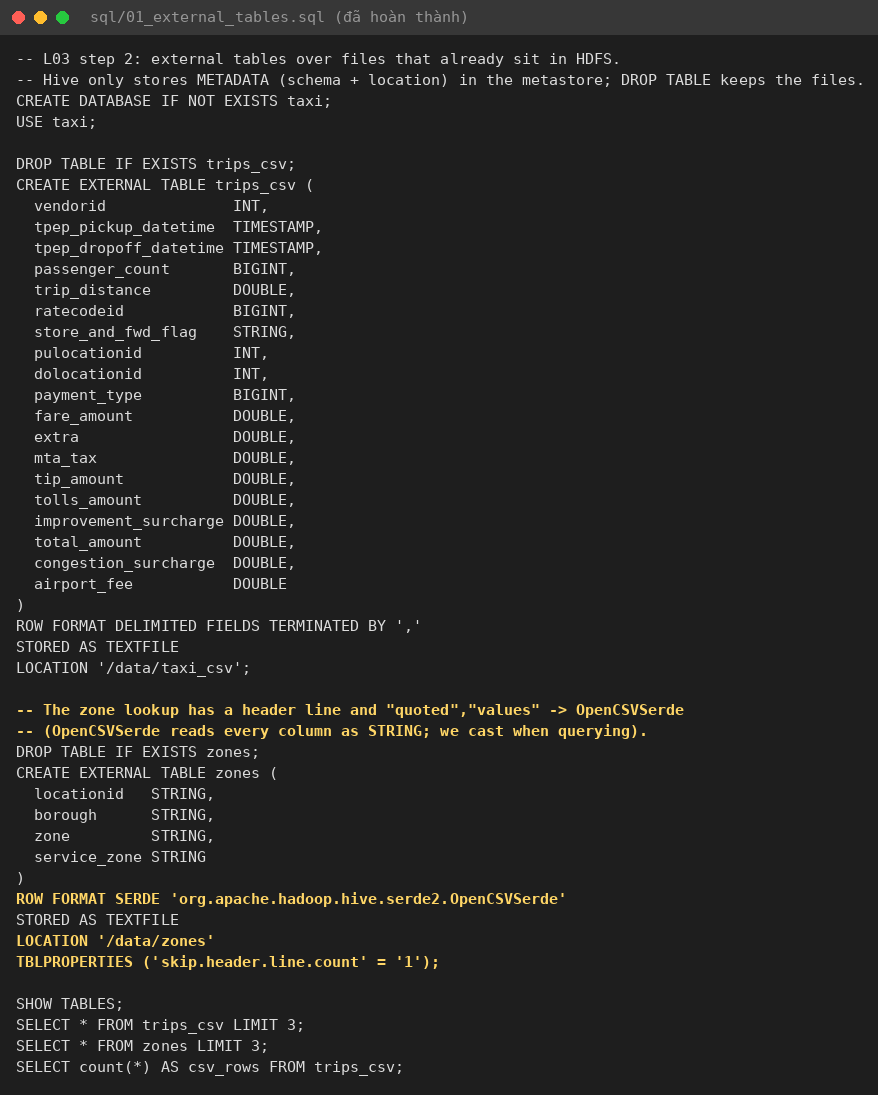
\includegraphics[keepaspectratio]{L03/img/code_01_external_tables.png}}
\pandocbounded{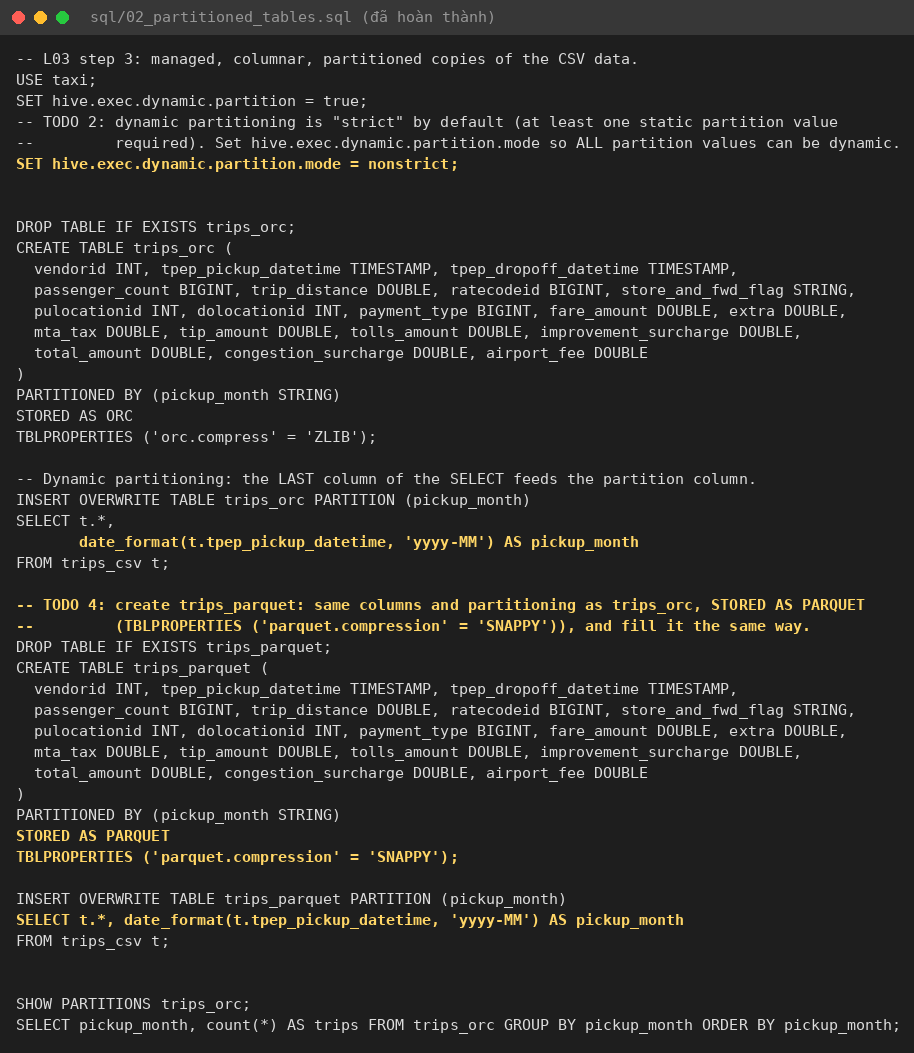
\includegraphics[keepaspectratio]{L03/img/code_02_partitioned_tables.png}}
\pandocbounded{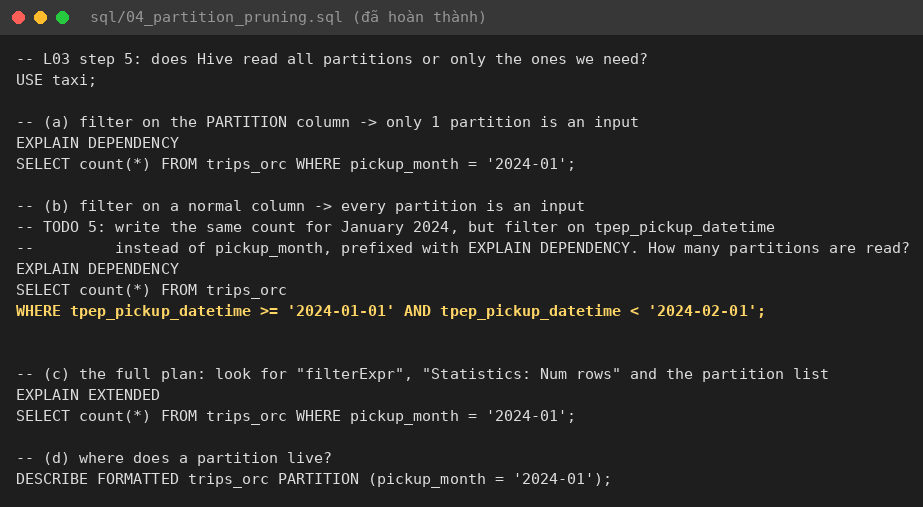
\includegraphics[keepaspectratio]{L03/img/code_04_partition_pruning.png}}
\pandocbounded{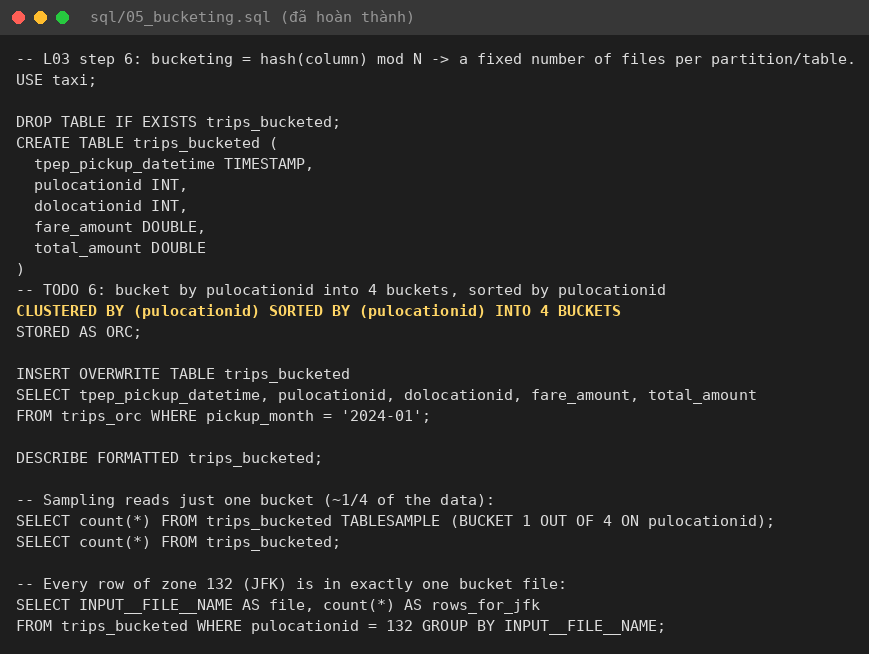
\includegraphics[keepaspectratio]{L03/img/code_05_bucketing.png}}

\subsection{1--2. Khởi động stack và đưa CSV lên
HDFS}\label{khux1edfi-ux111ux1ed9ng-stack-vuxe0-ux111ux1b0a-csv-luxean-hdfs}

\pandocbounded{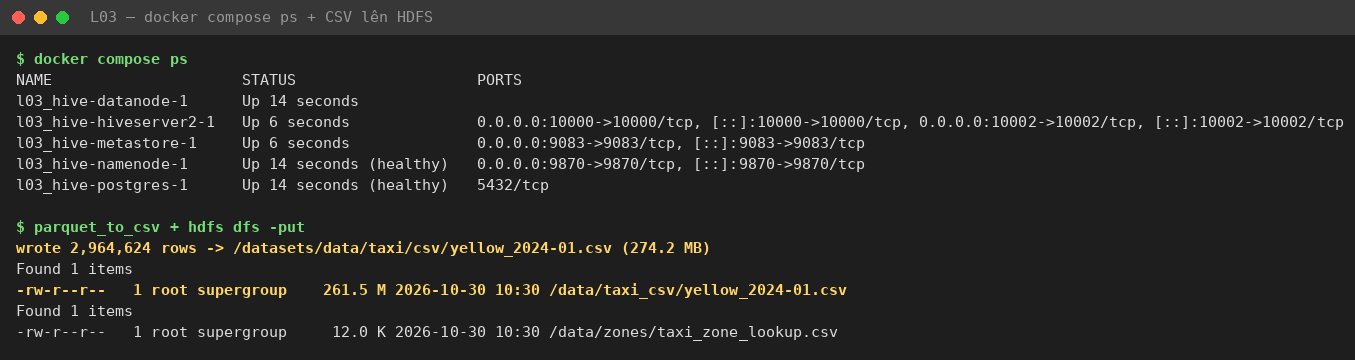
\includegraphics[keepaspectratio]{L03/img/01_stack_and_upload.png}}
\pandocbounded{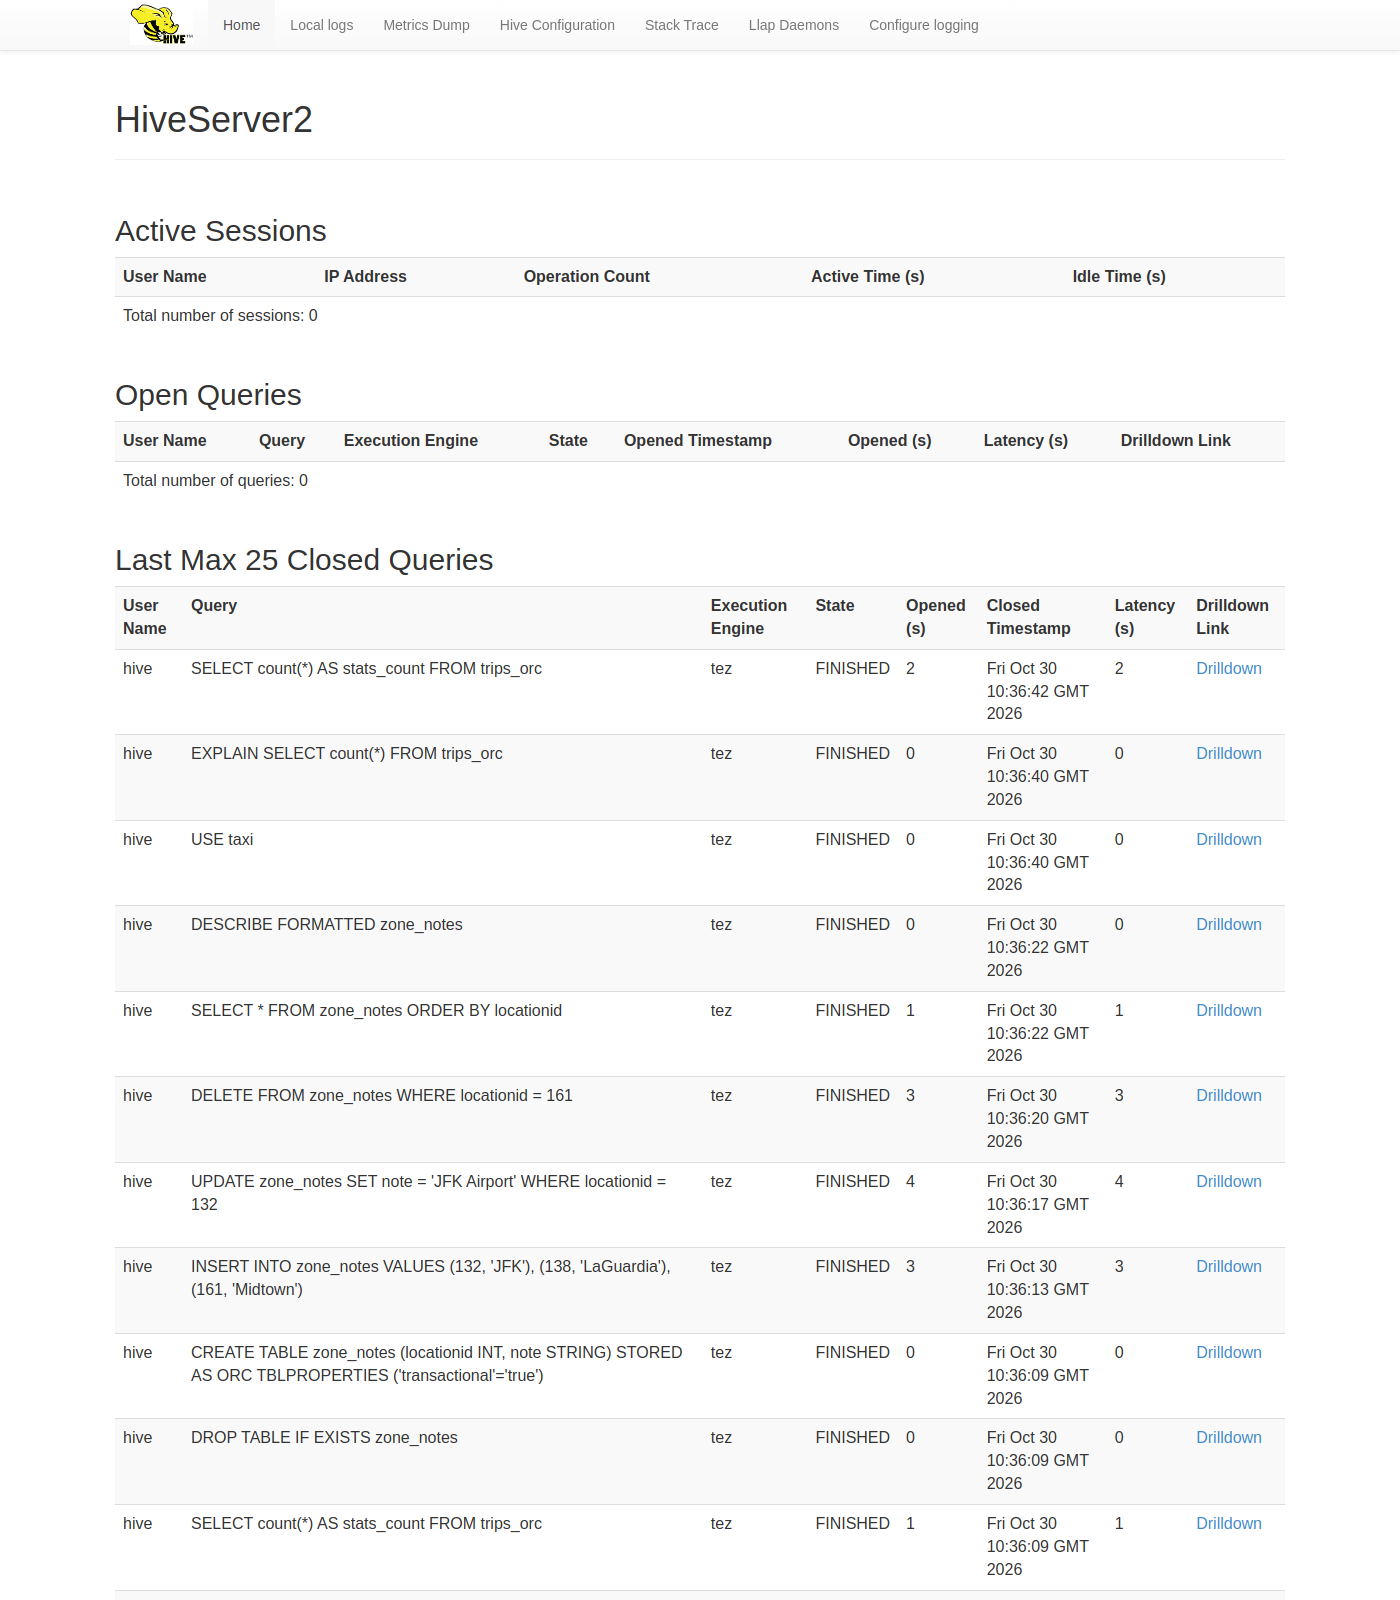
\includegraphics[keepaspectratio]{L03/img/20_ui_hiveserver2_home.png}}

\subsection{3. External tables}\label{external-tables}

3 dòng mẫu, 3 zone
(\texttt{1\ \textbar{}\ EWR\ \textbar{}\ Newark\ Airport\ \textbar{}\ EWR}\ldots),
\texttt{csv\_rows\ =\ 2,964,624}. Metastore (Postgres) chỉ lưu tên bảng,
kiểu bảng, \texttt{LOCATION} và \texttt{INPUT\_FORMAT}:

\begin{figure}
\centering
\pandocbounded{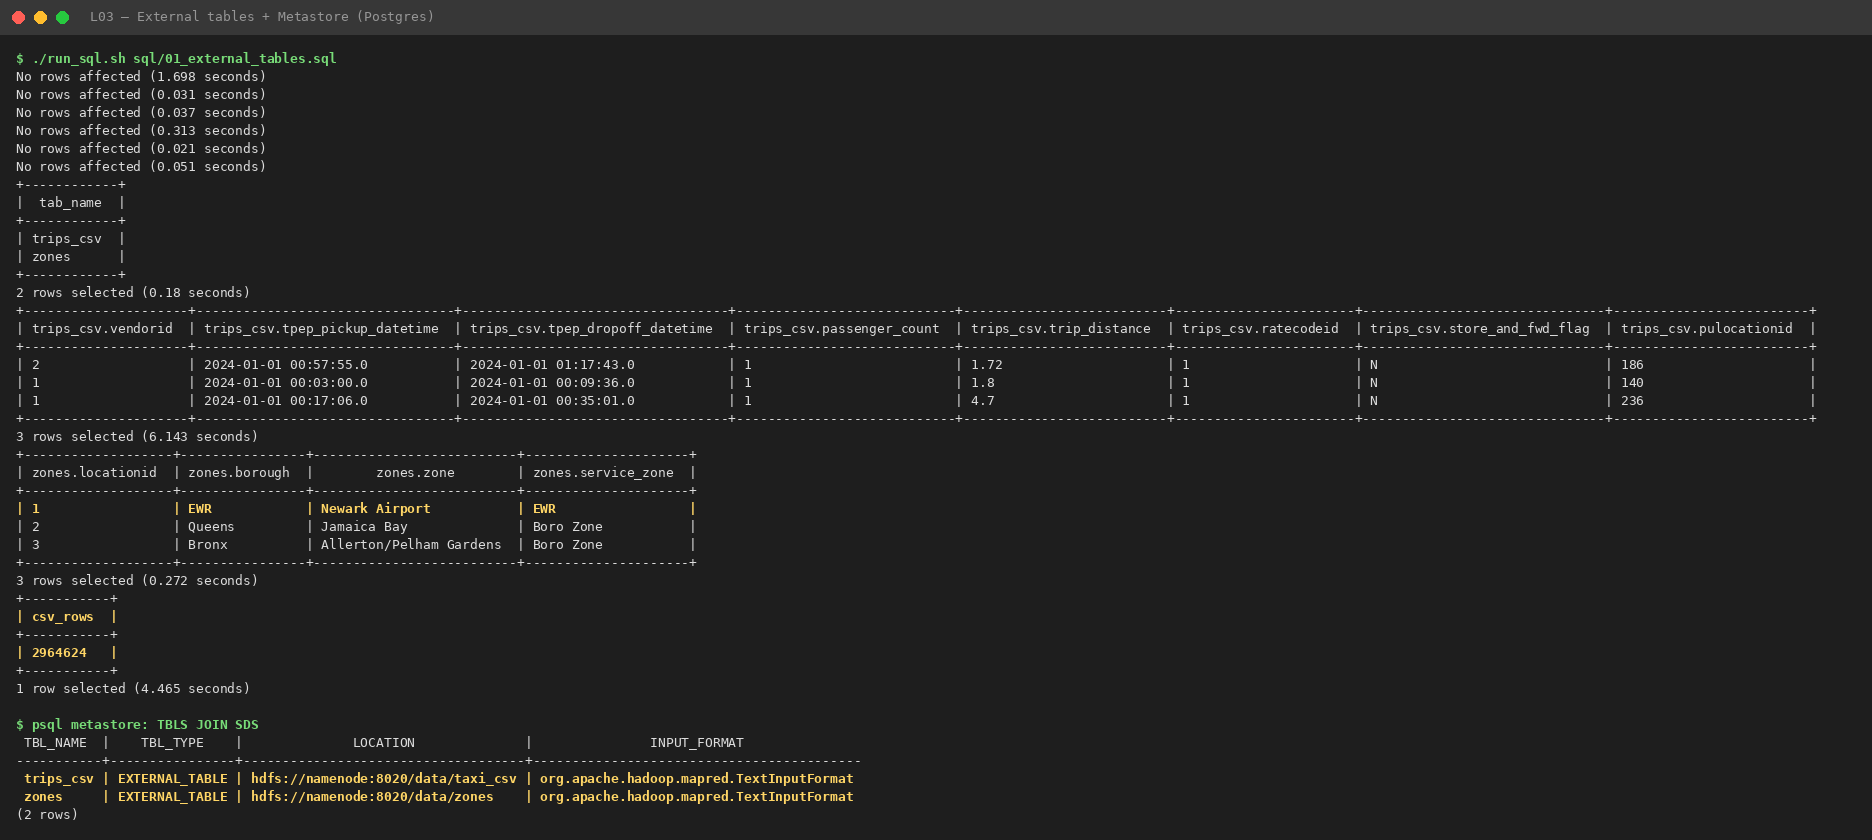
\includegraphics[keepaspectratio]{L03/img/02_external_tables_and_metastore.png}}
\caption{external + metastore}
\end{figure}

\subsection{4. Bảng partition ORC và
Parquet}\label{bux1ea3ng-partition-orc-vuxe0-parquet}

INSERT OVERWRITE: ORC 42.8 s, Parquet 45.1 s (2,964,624 dòng mỗi bảng).
\texttt{SHOW\ PARTITIONS} cho \textbf{5 partition} (dữ liệu cả tháng có
thêm 2024-02 so với mẫu 1 triệu dòng):

\begin{longtable}[]{@{}ll@{}}
\toprule\noalign{}
pickup\_month & trips \\
\midrule\noalign{}
\endhead
\bottomrule\noalign{}
\endlastfoot
2002-12 & 2 \\
2009-01 & 3 \\
2023-12 & 10 \\
2024-01 & 2,964,606 \\
2024-02 & 3 \\
\end{longtable}

\pandocbounded{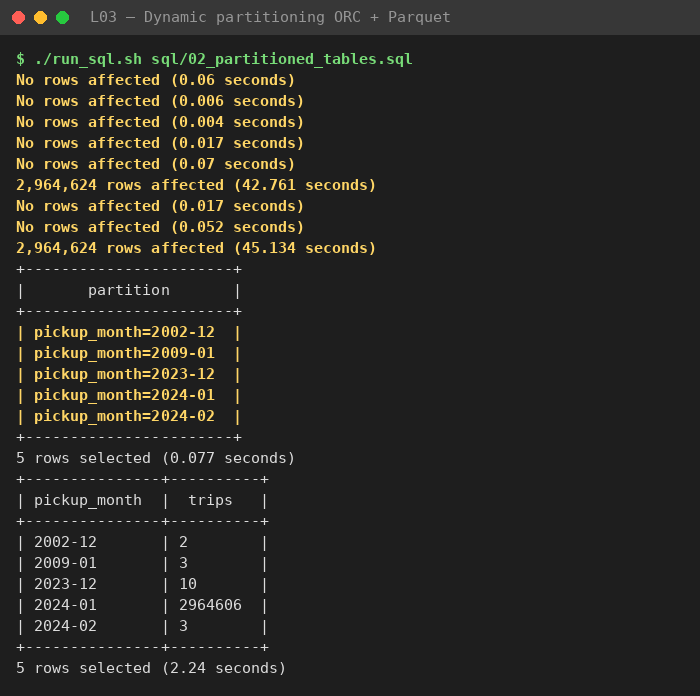
\includegraphics[keepaspectratio]{L03/img/03_partitioned_tables.png}}
\pandocbounded{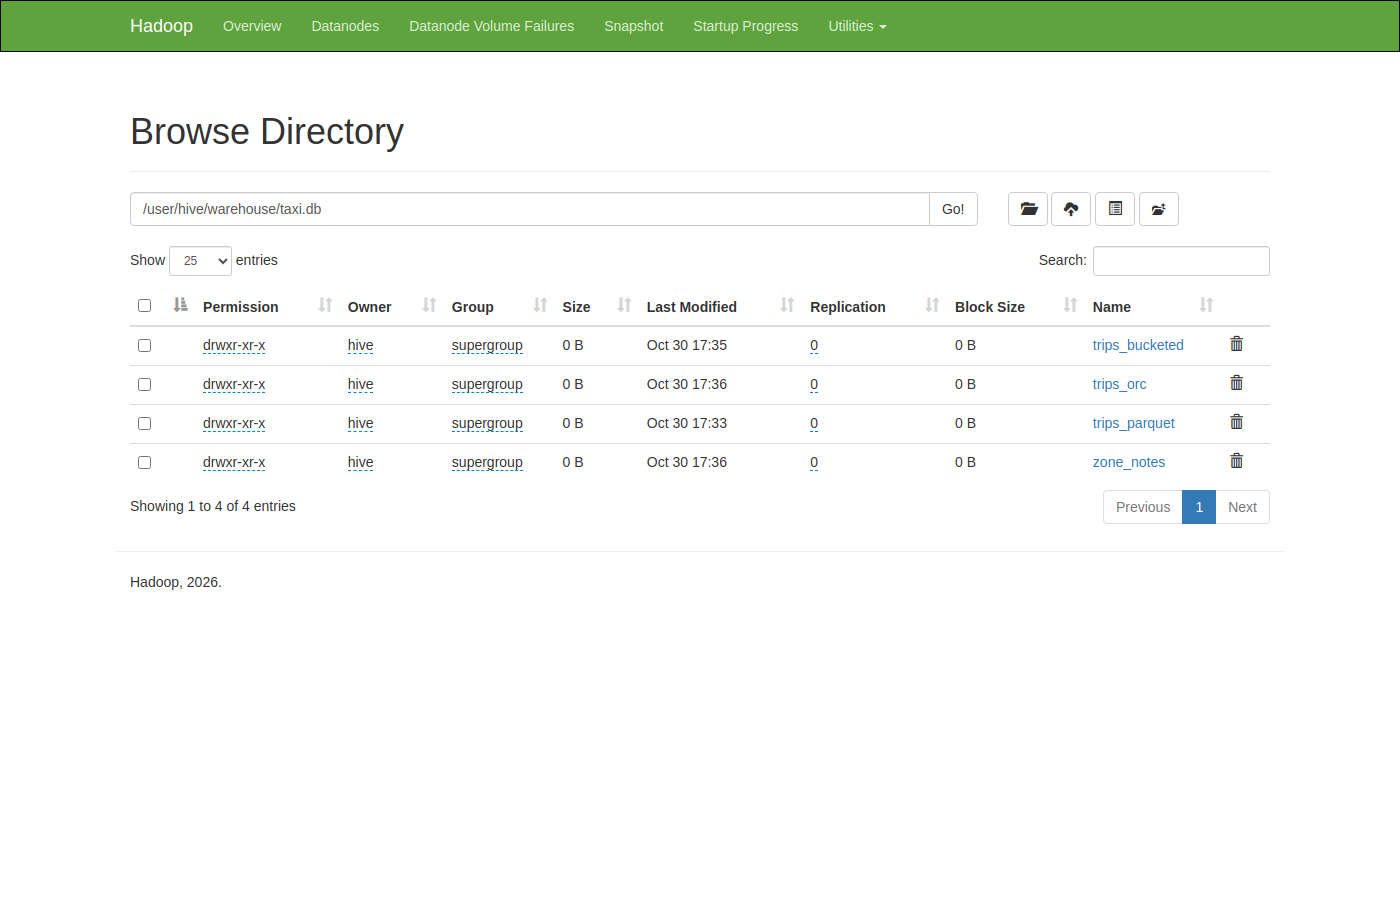
\includegraphics[keepaspectratio]{L03/img/21_ui_hdfs_warehouse_taxi_db.png}}
\pandocbounded{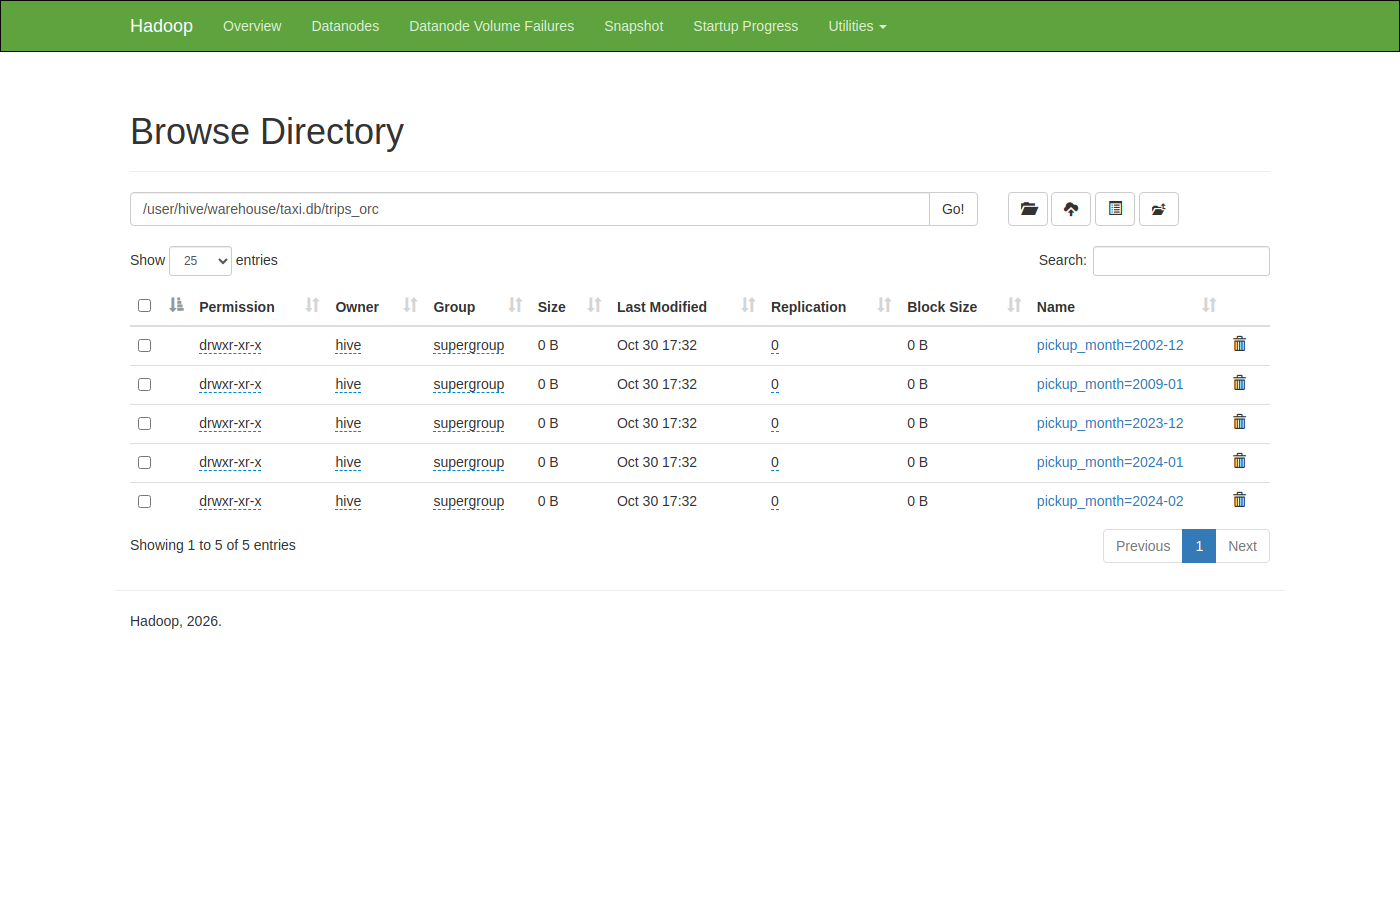
\includegraphics[keepaspectratio]{L03/img/22_ui_hdfs_trips_orc_partitions.png}}

\texttt{DESCRIBE\ FORMATTED\ trips\_orc} cho thấy
\texttt{Table\ Type:\ EXTERNAL\_TABLE},
\texttt{TRANSLATED\_TO\_EXTERNAL=TRUE},
\texttt{external.table.purge=TRUE} (đúng hành vi Hive 4 với bảng
``managed'' không phải ACID).

\begin{figure}
\centering
\pandocbounded{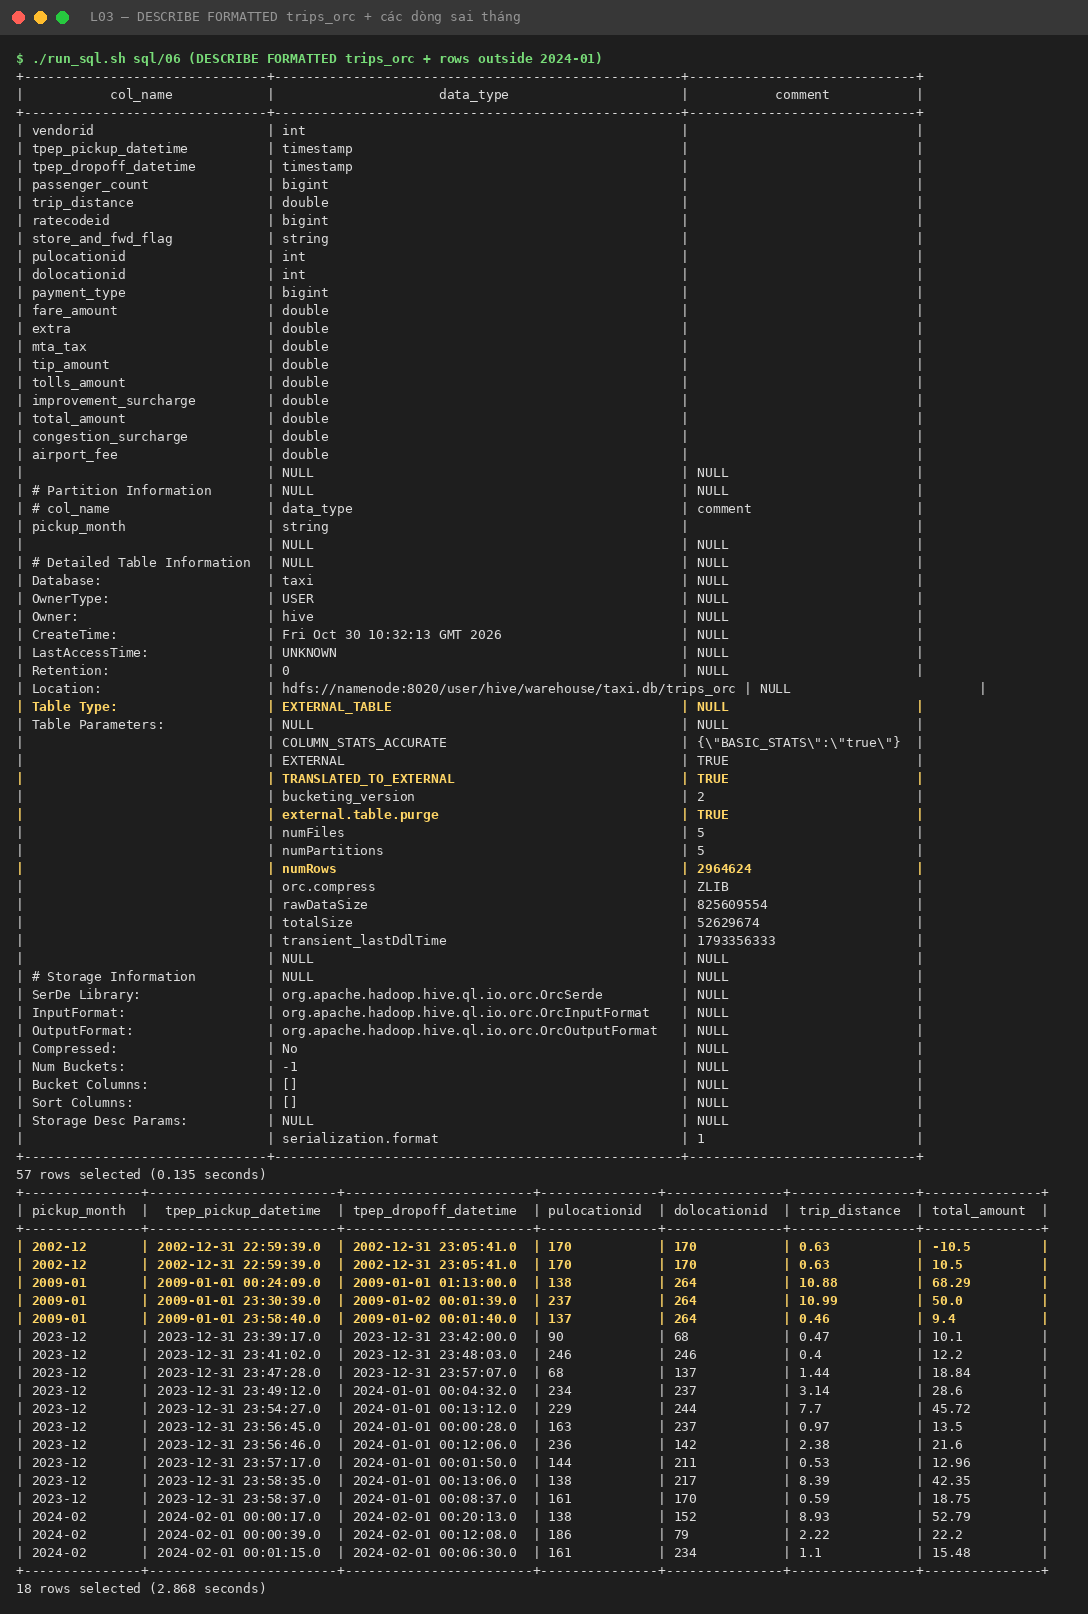
\includegraphics[keepaspectratio]{L03/img/05_describe_formatted_and_bad_rows.png}}
\caption{describe + bad rows}
\end{figure}

\subsubsection{Bảng kích thước}\label{bux1ea3ng-kuxedch-thux1b0ux1edbc}

\begin{longtable}[]{@{}lll@{}}
\toprule\noalign{}
Định dạng & Kích thước (cả tháng, 2.96 triệu dòng) & So với CSV \\
\midrule\noalign{}
\endhead
\bottomrule\noalign{}
\endlastfoot
CSV (text) & 274,217,811 B (261.5 MiB) & 1× \\
ORC + ZLIB & 52,629,674 B (50.2 MiB) & \textbf{5.2× nhỏ hơn} \\
Parquet + Snappy & 65,305,645 B (62.3 MiB) & \textbf{4.2× nhỏ hơn} \\
ORC bucketed (chỉ 5 cột) & 25,271,072 B (24.1 MiB) & 10.9× \\
\end{longtable}

\begin{figure}
\centering
\pandocbounded{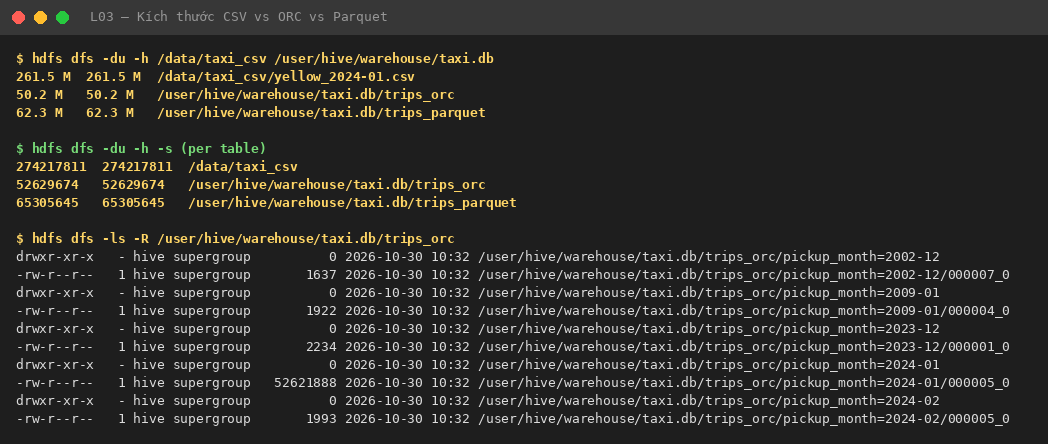
\includegraphics[keepaspectratio]{L03/img/04_sizes_csv_orc_parquet.png}}
\caption{sizes}
\end{figure}

\subsection{5. CSV, ORC và Parquet: bảng thời gian (lần chạy thứ
2)}\label{csv-orc-vuxe0-parquet-bux1ea3ng-thux1eddi-gian-lux1ea7n-chux1ea1y-thux1ee9-2}

\begin{longtable}[]{@{}
  >{\raggedright\arraybackslash}p{(\linewidth - 6\tabcolsep) * \real{0.2500}}
  >{\raggedright\arraybackslash}p{(\linewidth - 6\tabcolsep) * \real{0.2500}}
  >{\raggedright\arraybackslash}p{(\linewidth - 6\tabcolsep) * \real{0.2500}}
  >{\raggedright\arraybackslash}p{(\linewidth - 6\tabcolsep) * \real{0.2500}}@{}}
\toprule\noalign{}
\begin{minipage}[b]{\linewidth}\raggedright
Query
\end{minipage} & \begin{minipage}[b]{\linewidth}\raggedright
CSV
\end{minipage} & \begin{minipage}[b]{\linewidth}\raggedright
ORC
\end{minipage} & \begin{minipage}[b]{\linewidth}\raggedright
Parquet
\end{minipage} \\
\midrule\noalign{}
\endhead
\bottomrule\noalign{}
\endlastfoot
Q1 top pickup zones tháng 01/2024 & \textbf{8.53 s} & \textbf{1.89 s} &
\textbf{1.62 s} \\
Q2 join \texttt{zones} theo borough (ORC) & & 2.66 s & \\
\end{longtable}

(Lần chạy 1: 9.22 / 1.99 / 1.77 s.) Q1 dòng đầu: zone \texttt{132} (JFK)
có \textbf{145,240 chuyến}, avg fare \textbf{59.40}; ba nguồn cho kết
quả giống hệt nhau. Q2: Manhattan 2,646,933 chuyến (\textbf{89.3 \%}),
Queens 273,125, Brooklyn 25,258\ldots{}

\begin{figure}
\centering
\pandocbounded{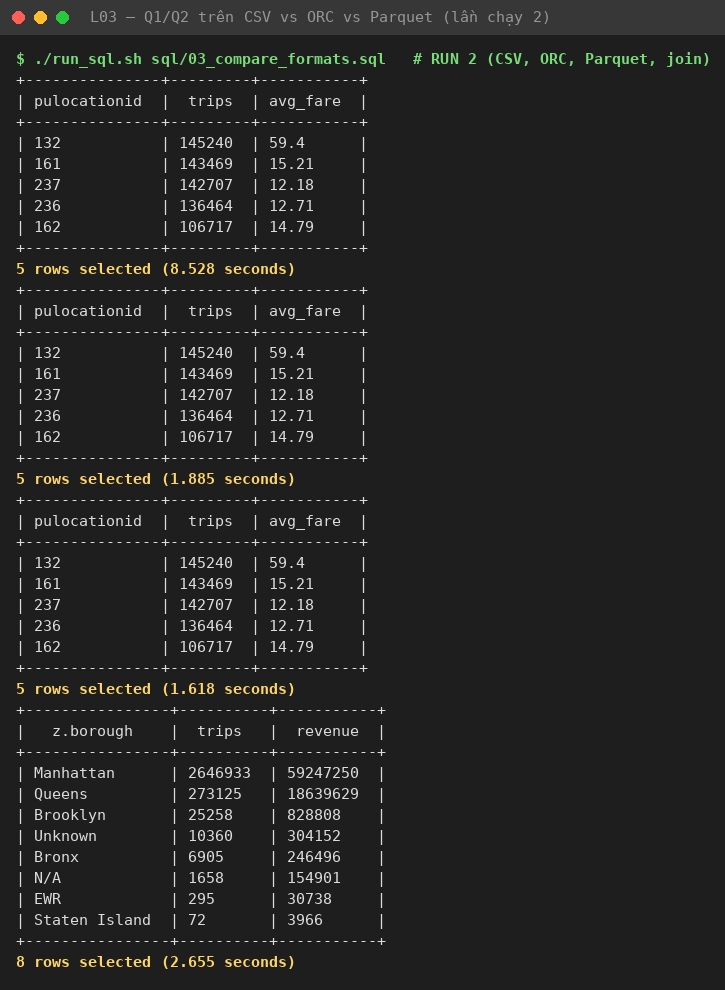
\includegraphics[keepaspectratio]{L03/img/06_compare_formats_run2.png}}
\caption{compare}
\end{figure}

\subsection{6. Partition pruning}\label{partition-pruning}

\begin{itemize}
\tightlist
\item
  \begin{enumerate}
  \def\labelenumi{(\alph{enumi})}
  \tightlist
  \item
    \texttt{WHERE\ pickup\_month\ =\ \textquotesingle{}2024-01\textquotesingle{}}
    → \texttt{input\_partitions} chỉ có \textbf{1} partition.
  \end{enumerate}
\item
  \begin{enumerate}
  \def\labelenumi{(\alph{enumi})}
  \setcounter{enumi}{1}
  \tightlist
  \item
    TODO 5, \texttt{WHERE\ tpep\_pickup\_datetime} trong tháng 1 →
    \textbf{cả 5} partition là input (Hive không suy được partition từ
    cột thường).
  \end{enumerate}
\item
  \begin{enumerate}
  \def\labelenumi{(\alph{enumi})}
  \setcounter{enumi}{2}
  \tightlist
  \item
    \texttt{EXPLAIN\ EXTENDED}:
    \texttt{filterExpr:\ (pickup\_month\ =\ \textquotesingle{}2024-01\textquotesingle{})},
    \texttt{Path\ -\textgreater{}\ Alias} chỉ có
    \texttt{.../trips\_orc/pickup\_month=2024-01}.
  \end{enumerate}
\end{itemize}

\begin{figure}
\centering
\pandocbounded{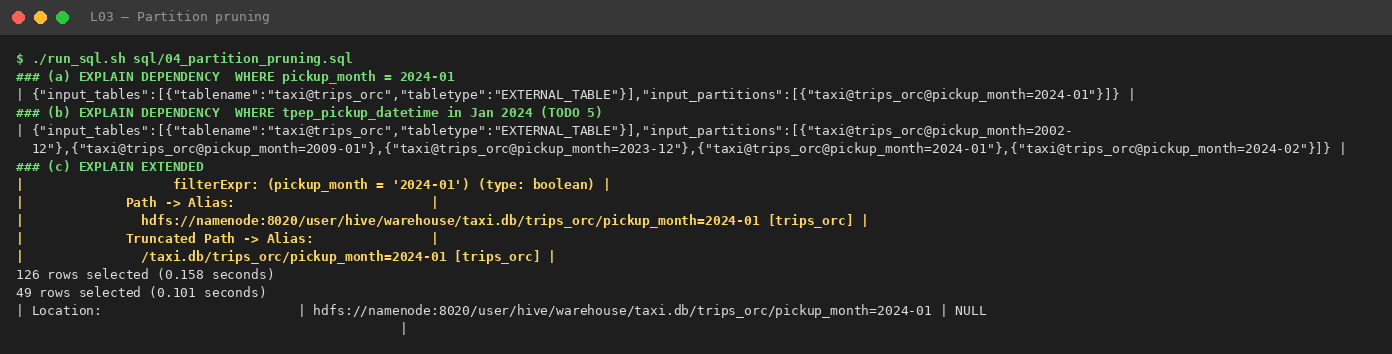
\includegraphics[keepaspectratio]{L03/img/07_partition_pruning.png}}
\caption{pruning}
\end{figure}

\subsection{7. Bucketing}\label{bucketing}

Đúng \textbf{4 file} \texttt{000000\_0\ …\ 000003\_0}.
\texttt{TABLESAMPLE(BUCKET\ 1\ OUT\ OF\ 4)} = 619,893 dòng
(\textasciitilde21 \%, vì bucket theo hash nên không đều). Cả
\textbf{145,240 dòng JFK} đều nằm trong \textbf{một} file
\texttt{000002\_0} (vì vậy file này lớn nhất, 8.1 MB).

\pandocbounded{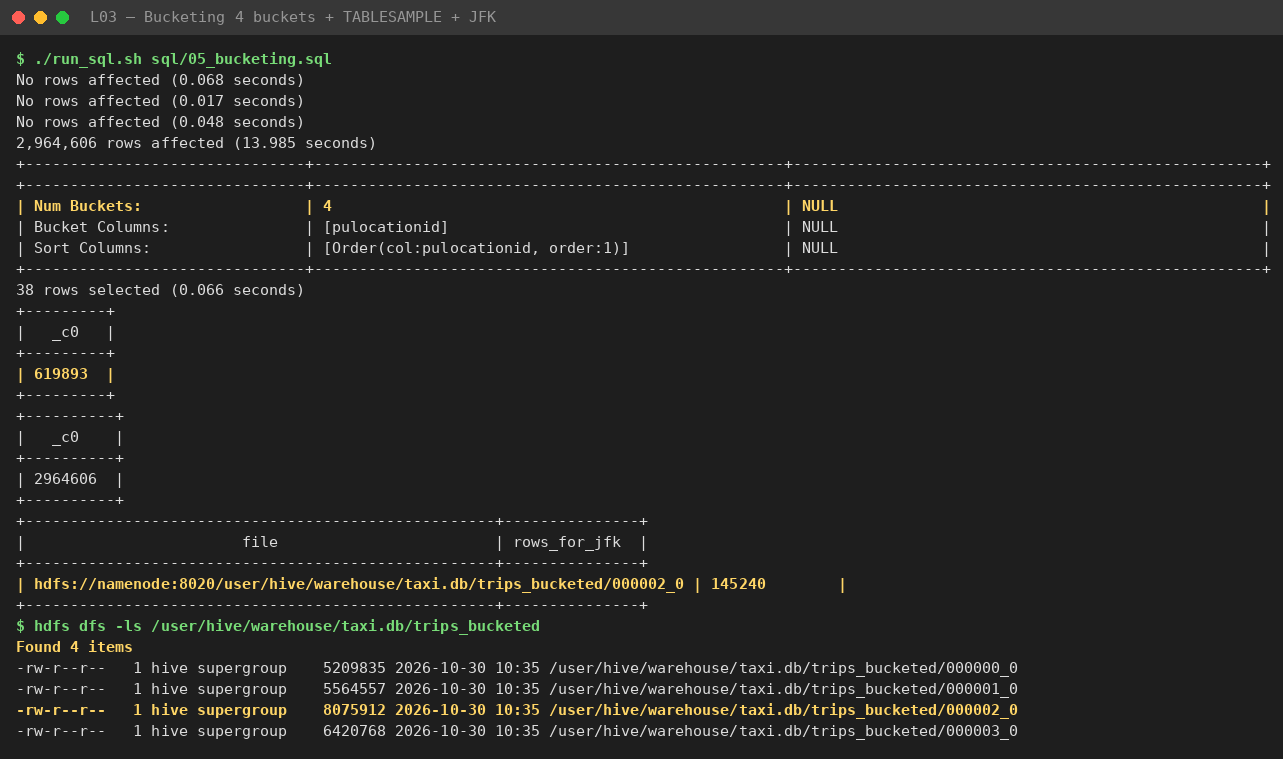
\includegraphics[keepaspectratio]{L03/img/08_bucketing.png}}
\pandocbounded{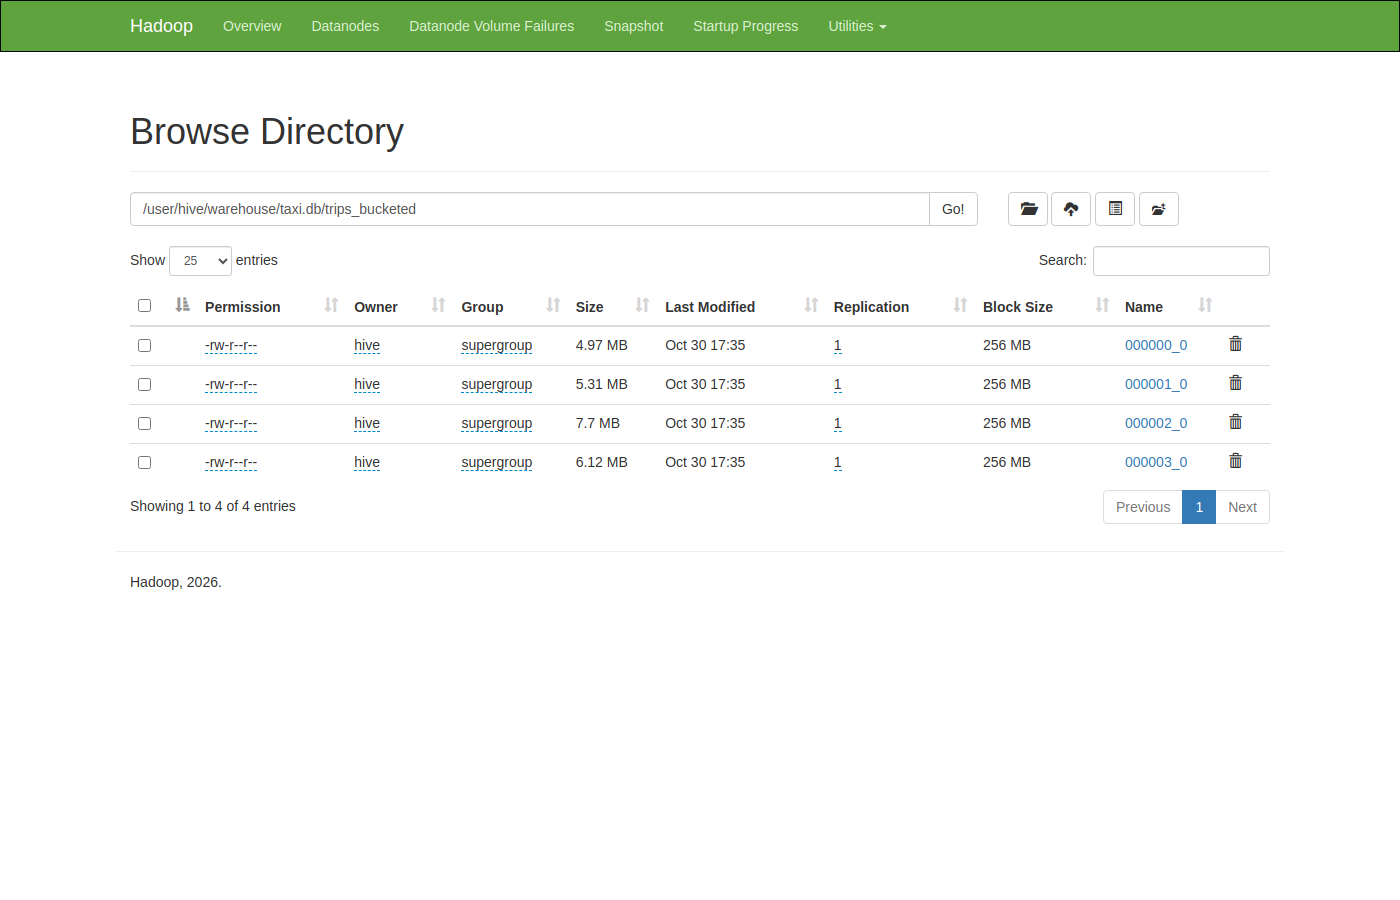
\includegraphics[keepaspectratio]{L03/img/23_ui_hdfs_trips_bucketed_4files.png}}

\subsection{Stretch}\label{stretch}

\textbf{ACID.} \texttt{zone\_notes} với \texttt{transactional=true} là
\texttt{MANAGED\_TABLE} thật. Sau INSERT, UPDATE rồi DELETE, HDFS có
\texttt{delta\_0000001} (insert), \texttt{delete\_delta\_0000002} +
\texttt{delta\_0000002} (UPDATE = xoá + ghi lại) và
\texttt{delete\_delta\_0000003} (DELETE). Không file nào bị sửa tại chỗ;
reader merge các delta khi đọc, compaction gộp chúng về sau.

\textbf{Statistics.}
\texttt{ANALYZE\ ...\ COMPUTE\ STATISTICS\ FOR\ COLUMNS} mất 18.4 s. Sau
đó, với \texttt{hive.compute.query.using.stats=true}, \texttt{count(*)}
\textbf{vẫn chạy DAG Tez} (EXPLAIN vẫn có \texttt{TableScan},
\textasciitilde1.6--2.6 s). Lý do: \texttt{trips\_orc} thực chất là bảng
\textbf{EXTERNAL} (translated), và Hive không tin stats của bảng
external để trả lời thay cho việc quét, vì file có thể bị thay đổi ngoài
Hive. Với bảng managed/ACID, câu trả lời sẽ lấy thẳng từ metastore (chỉ
còn Fetch, không có job).

\pandocbounded{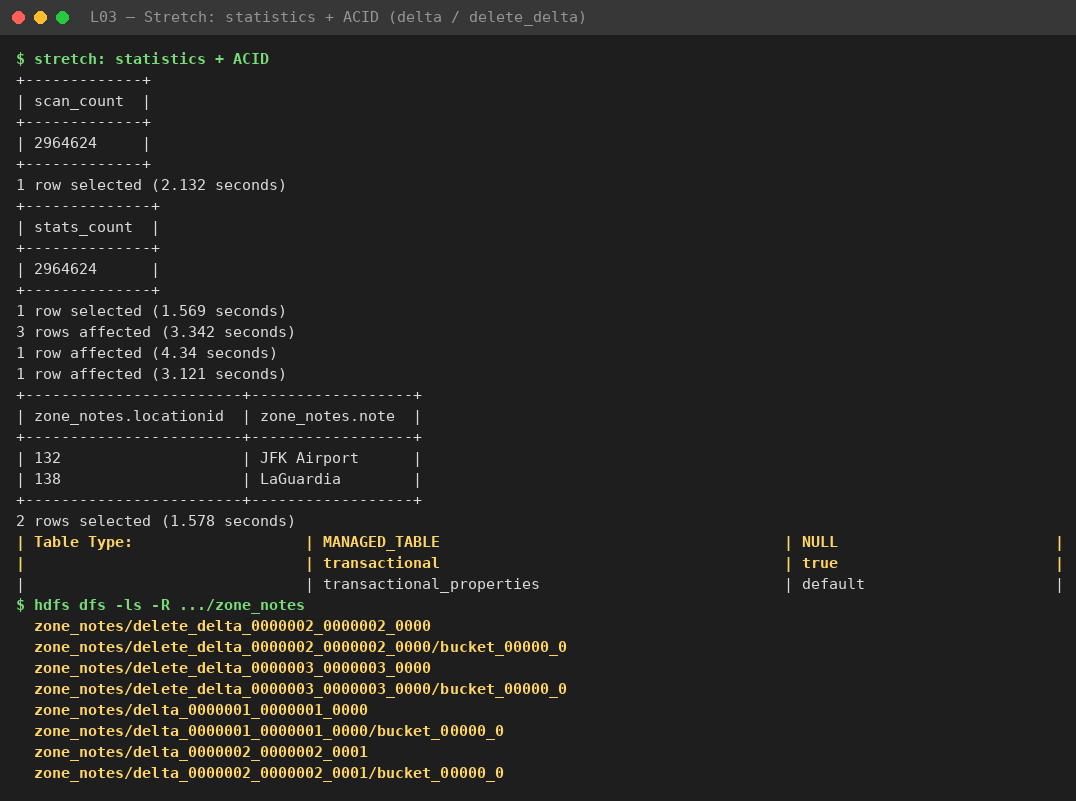
\includegraphics[keepaspectratio]{L03/img/09_stretch_stats_acid.png}}
\pandocbounded{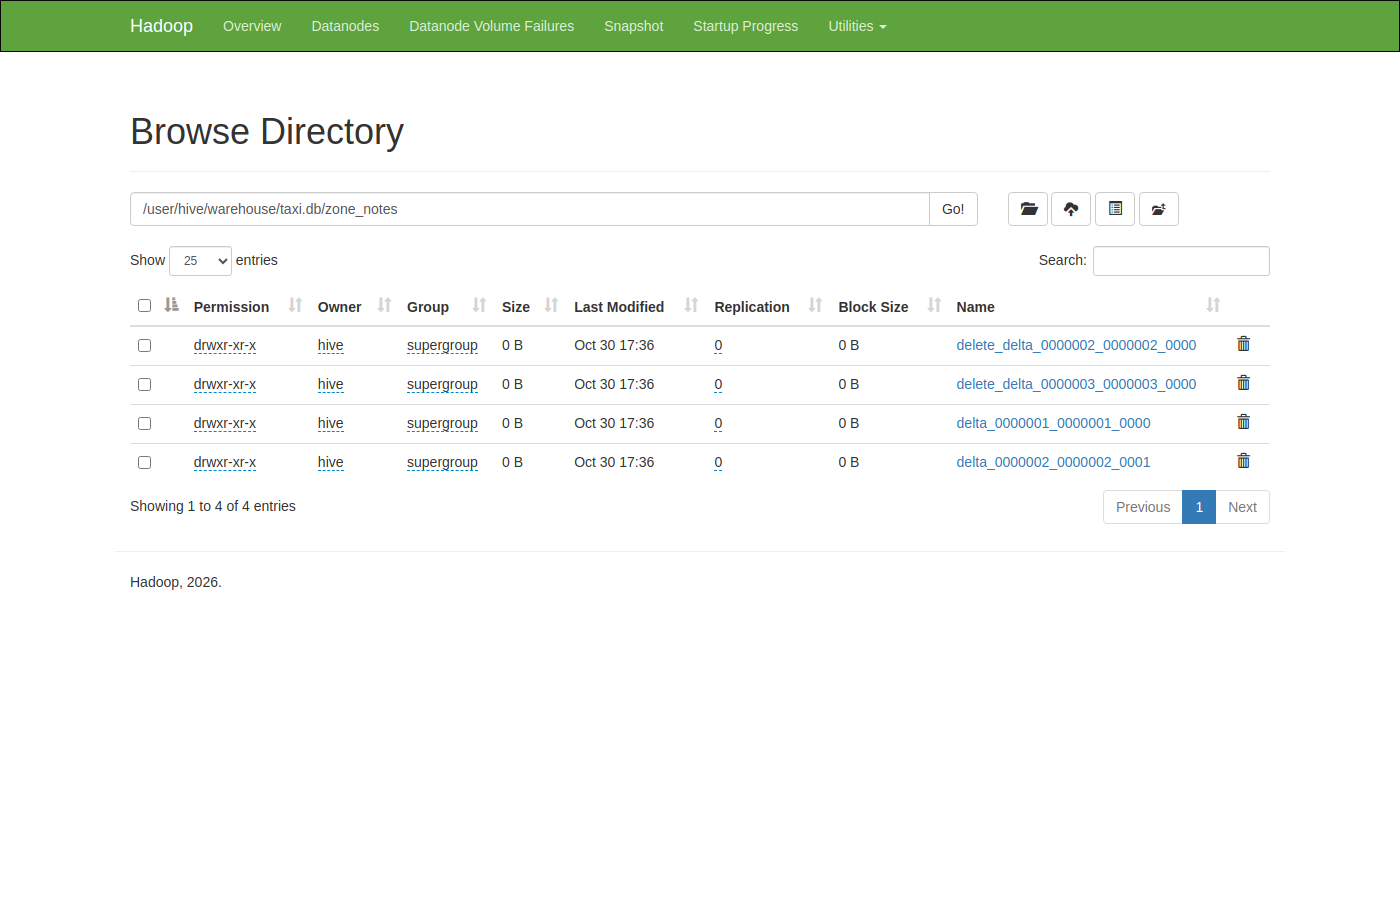
\includegraphics[keepaspectratio]{L03/img/24_ui_hdfs_zone_notes_acid_deltas.png}}

\subsection{Trả lời checkpoint}\label{trux1ea3-lux1eddi-checkpoint-2}

\textbf{Q1. Metastore lưu gì, HDFS lưu gì? DROP TABLE thì sao?}
\textbf{Metastore} (bảng \texttt{TBLS}, \texttt{SDS},
\texttt{PARTITIONS}\ldots{} trong Postgres): database, tên bảng, cột và
kiểu, SerDe, input/output format, kiểu bảng, \textbf{LOCATION} của bảng
và của từng partition, giá trị partition, thống kê (numRows,
totalSize\ldots), trạng thái ACID/transaction. \textbf{HDFS} chỉ chứa
file dữ liệu. \texttt{DROP\ TABLE\ trips\_csv} (external): chỉ xoá
metadata, file trong \texttt{/data/taxi\_csv} vẫn còn.
\texttt{DROP\ TABLE\ trips\_orc} (external +
\texttt{external.table.purge=TRUE}): xoá metadata \textbf{và} thư mục
\texttt{/user/hive/warehouse/taxi.db/trips\_orc}.

\textbf{Q3. Vì sao ORC/Parquet nhỏ hơn CSV 4--5 lần?} (thực đo 5.2× và
4.2×) (a) \textbf{Lưu theo cột}: giá trị cùng kiểu, cùng cột nằm cạnh
nhau nên các encoding dictionary, RLE, delta, bit-packing rất hiệu quả
(\texttt{vendorid}, \texttt{payment\_type}, \texttt{ratecodeid} chỉ có
vài giá trị khác nhau). (b) \textbf{Kiểu nhị phân + nén} (ZLIB/Snappy)
thay cho chữ số dạng text và dấu phân cách: một timestamp là 8 byte số
thay vì chuỗi 19 ký tự. ORC + ZLIB nén mạnh hơn Parquet + Snappy (Snappy
ưu tiên tốc độ hơn tỉ lệ nén).

\textbf{Q4. Vì sao Q1 nhanh hơn trên ORC/Parquet?} (8.53 s → 1.89 / 1.62
s, nhanh \textasciitilde4.5--5×) * \textbf{Column pruning}: Q1 chỉ cần
2--3 trong 19 cột (\texttt{pulocationid}, \texttt{fare\_amount}, cột
partition). ORC/Parquet chỉ đọc các column chunk đó, còn CSV phải đọc và
parse \textbf{toàn bộ} 274 MB, từng dòng. * \textbf{Partition pruning}:
với ORC/Parquet, filter nằm trên \texttt{pickup\_month}, nên Hive chỉ mở
thư mục \texttt{pickup\_month=2024-01} (đã chứng minh bằng EXPLAIN
DEPENDENCY, 1 so với 5 partition). Bảng CSV không có partition nên phải
quét hết rồi lọc theo timestamp. * \textbf{Predicate pushdown / min-max
statistics}: mỗi stripe/row group lưu min/max và có row index, nên
reader bỏ qua được các khối không thể khớp điều kiện. * Ngoài ra, reader
ORC/Parquet được \textbf{vectorized} (xử lý theo batch 1,024 dòng) và
không tốn công parse text thành số.

\textbf{Q6. Partition theo \texttt{pulocationid} + ngày? Theo
\texttt{tpep\_pickup\_datetime}?} \texttt{pulocationid} × ngày ≈ 265 ×
31 ≈ \textbf{8,000 partition mỗi tháng}, mỗi partition chỉ có một file
vài KB đến vài trăm KB. Đây là \textbf{small files problem}: NameNode
phải giữ hàng chục nghìn object trong heap, \textbf{Metastore} phải lưu
hàng nghìn dòng \texttt{PARTITIONS}/\texttt{SDS} (query planning chậm vì
phải liệt kê và lấy metadata partition), và mỗi file nhỏ thành một
split/task riêng nên overhead lấn át thời gian xử lý thật. Partition
theo timestamp gốc thì gần như \textbf{mỗi giây một partition}: hàng
triệu thư mục, file vài trăm byte, metastore và NameNode quá tải. Nguyên
tắc: partition theo cột có cardinality thấp mà query hay lọc, mỗi
partition nên chứa từ hàng trăm MB đến khoảng 1 GB.

\textbf{Q7. Partitioning hay bucketing? Vì sao bucketing có số file cố
định?} \textbf{Partitioning} tạo thư mục theo \textbf{giá trị} cột, dùng
cho cột cardinality thấp mà query hay lọc (ngày, tháng, quốc gia), để bỏ
qua cả thư mục khi đọc. \textbf{Bucketing} chia dữ liệu theo
\texttt{hash(col)\ mod\ N} vào N file, dùng cho cột cardinality cao (id,
\texttt{pulocationid}). Nó cho phép sampling (\texttt{TABLESAMPLE}),
bucket map join hoặc sort-merge-bucket join, và tránh shuffle khi hai
bảng được bucket giống nhau trên khoá join. Số file cố định vì \textbf{N
được chốt trong DDL} (\texttt{INTO\ 4\ BUCKETS}): mỗi dòng đi vào đúng
bucket \texttt{hash\ mod\ 4} bất kể dữ liệu nhiều hay ít (thực nghiệm:
đúng 4 file, mọi dòng JFK nằm trong \texttt{000002\_0}).

\textbf{Q2.} Trong file trips, \texttt{ROW\ FORMAT\ DELIMITED}
(LazySimpleSerDe) chỉ tách theo dấu phẩy, đủ dùng vì không có ngoặc kép
hay header. File zones có header và
\texttt{"giá\ trị\ trong\ ngoặc\ kép"} (ví dụ
\texttt{"Allerton/Pelham\ Gardens"}), nên cần \texttt{OpenCSVSerde}.
Nhược điểm của nó: \textbf{mọi cột đều là STRING} (phải tự CAST, như
\texttt{CAST(z.locationid\ AS\ INT)} trong Q2), parse chậm hơn, không xử
lý NULL đặc biệt.

\textbf{Q5.} Partition tĩnh ghi giá trị ngay trong câu lệnh
(\texttt{PARTITION\ (pickup\_month=\textquotesingle{}2024-01\textquotesingle{})}).
Partition động lấy giá trị từ dữ liệu (cột cuối của SELECT). Mặc định là
\texttt{strict} (bắt buộc ít nhất một giá trị tĩnh) để một câu query lỗi
không vô tình tạo hàng nghìn partition, file và object trong metastore.
Lab đã thấy điều này ở quy mô nhỏ: các dòng 2002/2009 sinh ra partition
``lạ''.

\textbf{Q8.} Có 18 dòng ngoài tháng 01/2024: 2 dòng 2002-12-31 (một cặp
+10.5/−10.5, tức một chuyến bị hoàn tiền), 3 dòng 2009-01-01, 10 dòng
2023-12-31 23:39--23:58 (chuyến bắt đầu trước nửa đêm giao thừa) và 3
dòng 2024-02-01 00:00 (chuyến bắt đầu ngay sau nửa đêm). Các dòng năm
2002/2009 là lỗi đồng hồ thiết bị, còn các dòng 2023-12 và 2024-02 là
chuyến thật nằm ở biên tháng. Trong pipeline thật: kiểm tra event time
so với tháng của file nguồn; đưa dòng ngoài khoảng hợp lệ vào bảng
\textbf{quarantine/rejected} kèm lý do và đếm/cảnh báo; các dòng biên
tháng hợp lệ thì ghi vào đúng partition (hoặc giữ lại theo tháng của
file); không để dynamic partitioning âm thầm tạo partition rác.

\newpage

\section{L04 --- Ingestion: Sqoop và Spark JDBC từ PostgreSQL vào
HDFS}\label{l04-ingestion-sqoop-vuxe0-spark-jdbc-tux1eeb-postgresql-vuxe0o-hdfs}

Stack L04 gồm PostgreSQL (nguồn Olist, 6 bảng), HDFS, YARN, JobHistory,
Sqoop 1.4.7 và Spark. Log gốc nằm trong các file \texttt{0*.txt}, ảnh ở
\texttt{img/}.

\subsection{File nộp}\label{file-nux1ed9p-1}

\begin{longtable}[]{@{}
  >{\raggedright\arraybackslash}p{(\linewidth - 2\tabcolsep) * \real{0.5000}}
  >{\raggedright\arraybackslash}p{(\linewidth - 2\tabcolsep) * \real{0.5000}}@{}}
\toprule\noalign{}
\begin{minipage}[b]{\linewidth}\raggedright
File
\end{minipage} & \begin{minipage}[b]{\linewidth}\raggedright
Nội dung
\end{minipage} \\
\midrule\noalign{}
\endhead
\bottomrule\noalign{}
\endlastfoot
\texttt{sqoop\_part1.sh} & Các lệnh Sqoop phần 1: explore, full import,
TODO 1.2 (customers), append, lastmodified, saved job \\
\texttt{spark\_jdbc\_ingest.py} & TODO 1--5: đọc JDBC song song, ghi
Parquet phân vùng, incremental theo watermark, dedup snapshot \\
\texttt{01}--\texttt{09\_*.txt} & Log từng bước, kể cả log query phía
PostgreSQL \\
\end{longtable}

\begin{figure}
\centering
\pandocbounded{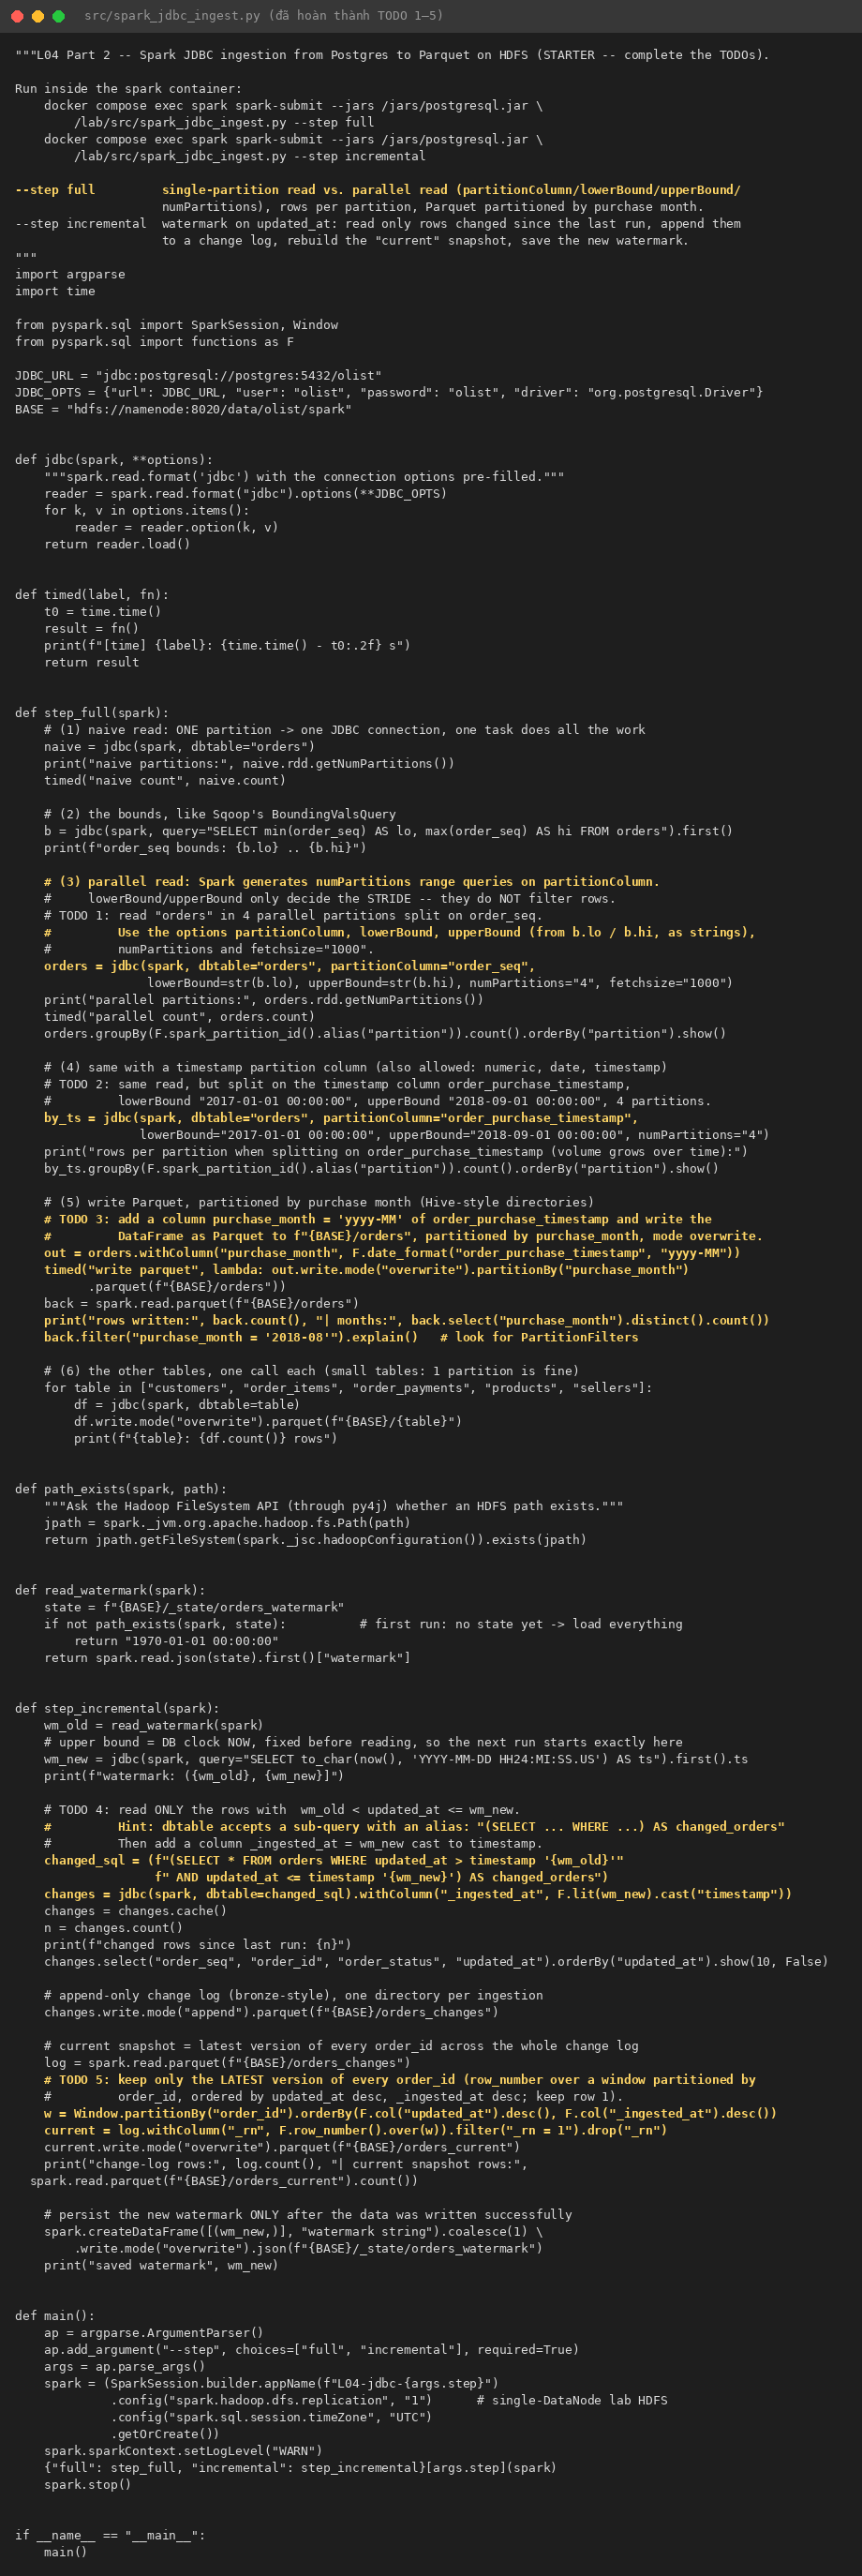
\includegraphics[keepaspectratio]{L04/img/code_spark_jdbc_ingest.png}}
\caption{spark\_jdbc\_ingest.py}
\end{figure}

\subsection{1. Nguồn dữ liệu}\label{nguux1ed3n-dux1eef-liux1ec7u}

Có 6 bảng. \texttt{orders} có 5,000 dòng, \texttt{order\_seq} chạy từ 1
đến 5000 và \texttt{max(updated\_at)} là \texttt{2018-09-08\ 09:48:29}.
Theo trạng thái: delivered 4,793, shipped 102, \ldots{}

\begin{figure}
\centering
\pandocbounded{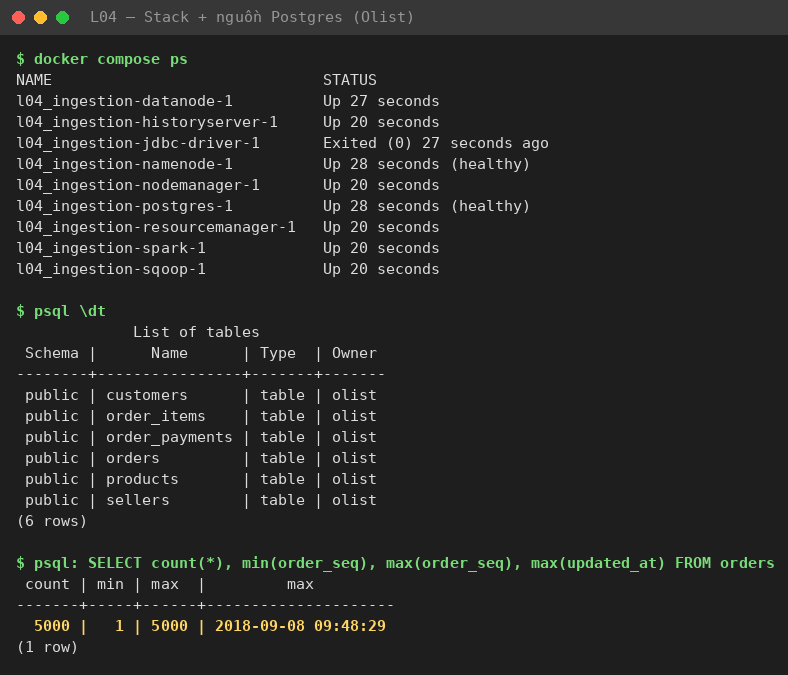
\includegraphics[keepaspectratio]{L04/img/01_stack_and_source.png}}
\caption{stack and source}
\end{figure}

\subsection{2. Sqoop full import và cách chia
split}\label{sqoop-full-import-vuxe0-cuxe1ch-chia-split}

\texttt{sqoop\ import\ -\/-table\ orders\ -\/-split-by\ order\_seq\ -m\ 4}:

\begin{itemize}
\tightlist
\item
  Sqoop chạy \texttt{BoundingValsQuery}
  (\texttt{SELECT\ MIN(order\_seq),\ MAX(order\_seq)\ FROM\ orders}),
  được (1, 5000), rồi chia thành 4 khoảng đều nhau.
\item
  Log PostgreSQL ghi lại đúng 4 câu query:
\end{itemize}

\begin{longtable}[]{@{}lll@{}}
\toprule\noalign{}
Map & Điều kiện WHERE & Số dòng \\
\midrule\noalign{}
\endhead
\bottomrule\noalign{}
\endlastfoot
0 &
\texttt{order\_seq\ \textgreater{}=\ 1\ AND\ order\_seq\ \textless{}\ 1251}
& 1,250 \\
1 &
\texttt{order\_seq\ \textgreater{}=\ 1251\ AND\ order\_seq\ \textless{}\ 2501}
& 1,250 \\
2 &
\texttt{order\_seq\ \textgreater{}=\ 2501\ AND\ order\_seq\ \textless{}\ 3751}
& 1,250 \\
3 &
\texttt{order\_seq\ \textgreater{}=\ 3751\ AND\ order\_seq\ \textless{}=\ 5000}
& 1,250 \\
\end{longtable}

\begin{itemize}
\tightlist
\item
  Đã chuyển 1.009 MB trong 25.23 s (thời gian MR); tổng thời gian lệnh
  CLI là 28.5 s.
\item
  4 file \texttt{part-m-0000x} chia đều nhau.
\end{itemize}

\pandocbounded{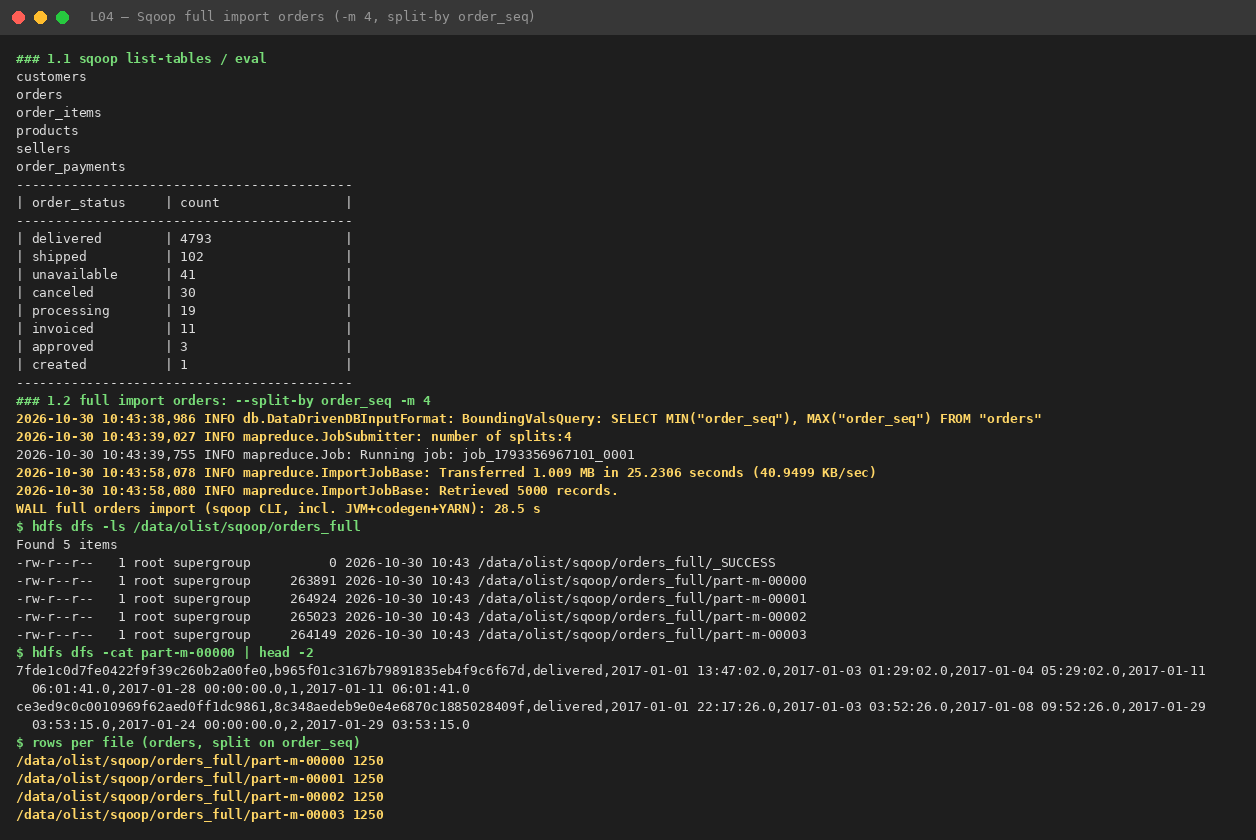
\includegraphics[keepaspectratio]{L04/img/02_sqoop_full_import_orders.png}}
\pandocbounded{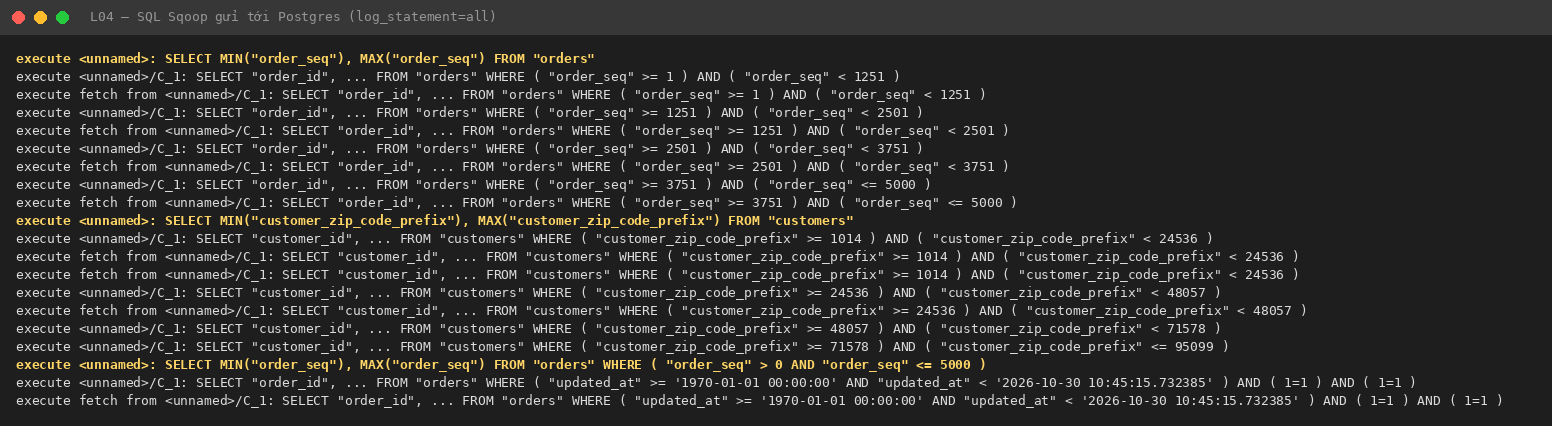
\includegraphics[keepaspectratio]{L04/img/05_postgres_log_sqoop_sql.png}}
\pandocbounded{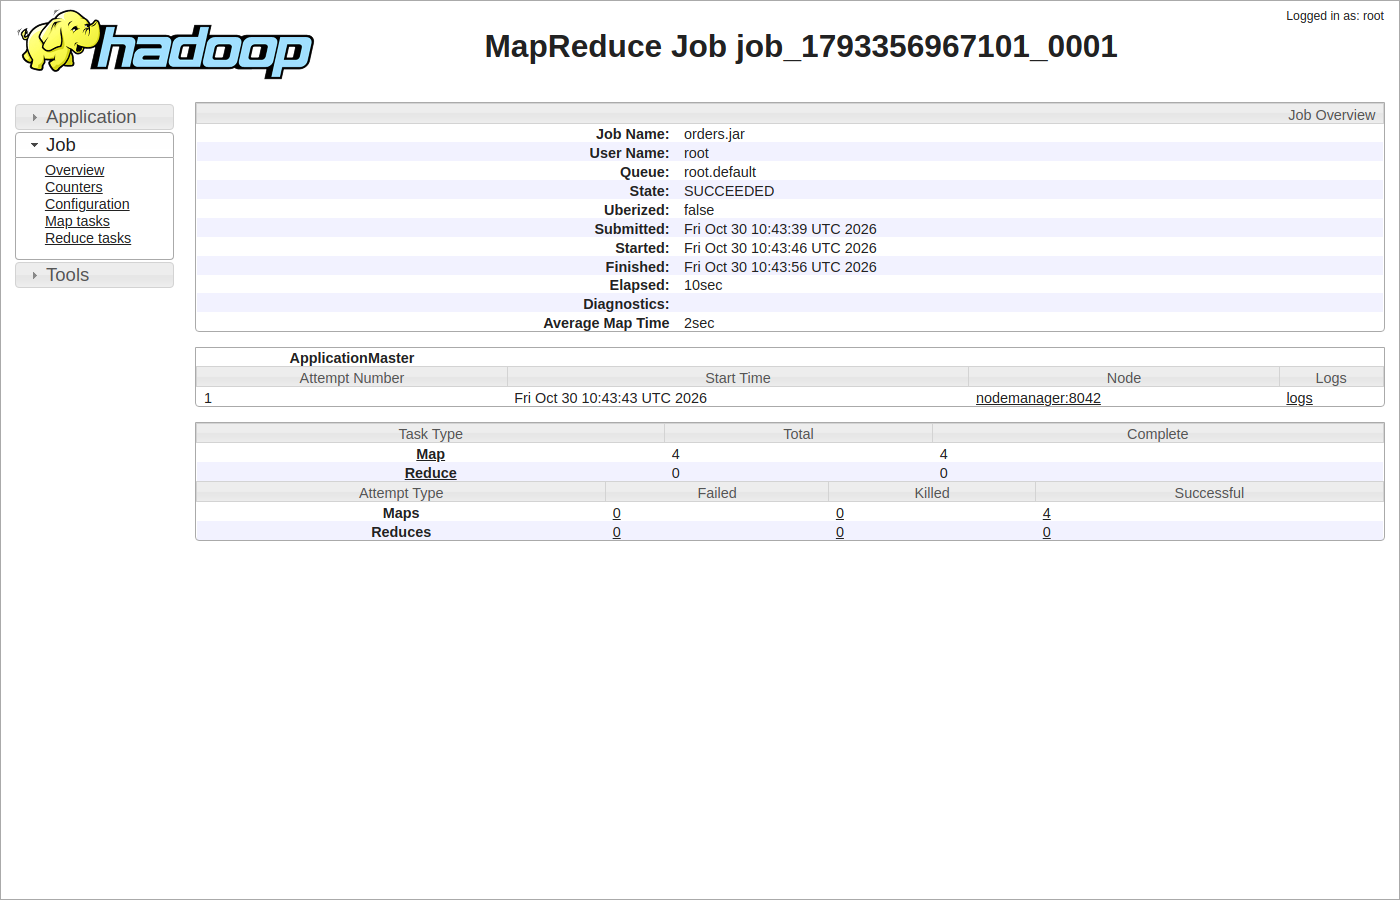
\includegraphics[keepaspectratio]{L04/img/24_ui_jobhistory_orders_full_4maps.png}}

\subsubsection{\texorpdfstring{TODO 1.2:
\texttt{customers\ -\/-split-by\ customer\_zip\_code\_prefix\ -m\ 4}}{TODO 1.2: customers -\/-split-by customer\_zip\_code\_prefix -m 4}}\label{todo-1.2-customers---split-by-customer_zip_code_prefix--m-4}

\begin{longtable}[]{@{}
  >{\raggedright\arraybackslash}p{(\linewidth - 8\tabcolsep) * \real{0.2000}}
  >{\raggedright\arraybackslash}p{(\linewidth - 8\tabcolsep) * \real{0.2000}}
  >{\raggedright\arraybackslash}p{(\linewidth - 8\tabcolsep) * \real{0.2000}}
  >{\raggedright\arraybackslash}p{(\linewidth - 8\tabcolsep) * \real{0.2000}}
  >{\raggedright\arraybackslash}p{(\linewidth - 8\tabcolsep) * \real{0.2000}}@{}}
\toprule\noalign{}
\begin{minipage}[b]{\linewidth}\raggedright
Bảng / cột split
\end{minipage} & \begin{minipage}[b]{\linewidth}\raggedright
part-m-00000
\end{minipage} & \begin{minipage}[b]{\linewidth}\raggedright
part-m-00001
\end{minipage} & \begin{minipage}[b]{\linewidth}\raggedright
part-m-00002
\end{minipage} & \begin{minipage}[b]{\linewidth}\raggedright
part-m-00003
\end{minipage} \\
\midrule\noalign{}
\endhead
\bottomrule\noalign{}
\endlastfoot
\texttt{orders} / \texttt{order\_seq} (1--5000) & 1,250 & 1,250 & 1,250
& 1,250 \\
\texttt{customers} / \texttt{customer\_zip\_code\_prefix} (1014--95099)
& \textbf{2,450} & 1,146 & \textbf{427} & 977 \\
\end{longtable}

Khoảng zip được chia đều tại 24536, 48057 và 71578, nhưng zip code tập
trung ở vùng São Paulo (01xxx--19xxx). Vì vậy split đầu nhận gần một nửa
số dòng, còn split thứ ba chỉ nhận 427 dòng: \textbf{data skew}.

\begin{figure}
\centering
\pandocbounded{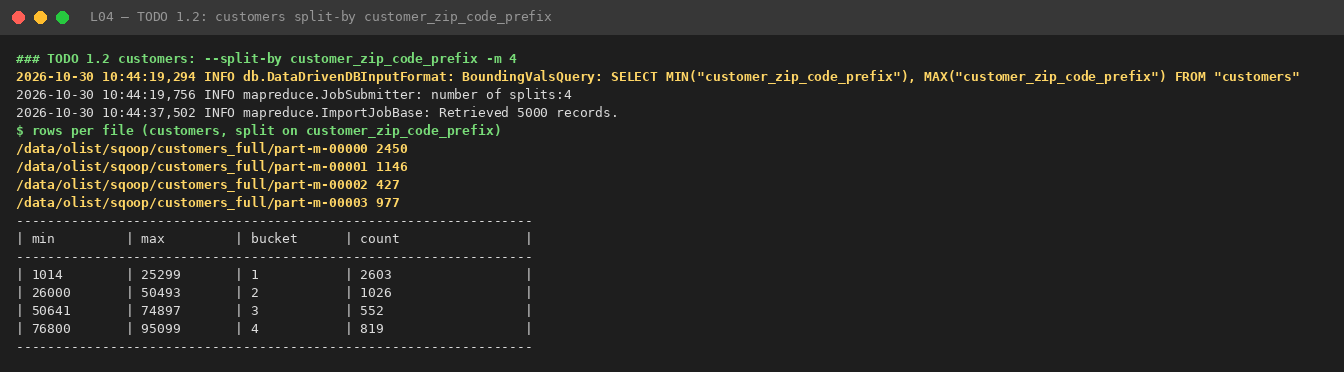
\includegraphics[keepaspectratio]{L04/img/03_sqoop_customers_skew_TODO1.2.png}}
\caption{customers skew}
\end{figure}

\subsection{3. Sqoop incremental: append, lastmodified, saved job,
merge,
export}\label{sqoop-incremental-append-lastmodified-saved-job-merge-export}

\begin{longtable}[]{@{}
  >{\raggedright\arraybackslash}p{(\linewidth - 2\tabcolsep) * \real{0.5000}}
  >{\raggedright\arraybackslash}p{(\linewidth - 2\tabcolsep) * \real{0.5000}}@{}}
\toprule\noalign{}
\begin{minipage}[b]{\linewidth}\raggedright
Bước
\end{minipage} & \begin{minipage}[b]{\linewidth}\raggedright
Kết quả
\end{minipage} \\
\midrule\noalign{}
\endhead
\bottomrule\noalign{}
\endlastfoot
Append, lần nạp đầu & lower 0, upper 5000 → 5,000 dòng; Sqoop gợi ý
\texttt{-\/-last-value\ 5000} \\
Lastmodified, baseline & 5,000 dòng; last-value
\texttt{2026-10-30\ 10:45:15.732385} \\
Saved job \texttt{orders\_incr} &
\texttt{incremental.last.value\ =\ 5000} lưu trong metastore của
Sqoop \\
\texttt{simulate\_changes} \#1 & tạo \texttt{order\_seq} 5001--5003; cập
nhật đơn 139 và 278 thành \texttt{delivered} \\
\texttt{sqoop\ job\ -\/-exec\ orders\_incr} & lower 5000, upper 5003 →
lấy \textbf{3} dòng; \texttt{last.value} thành 5003; tổng 5,003 dòng \\
Lastmodified + \texttt{-\/-merge-key\ order\_id} & lấy \textbf{5} dòng
(3 mới + 2 cập nhật); merge job → một \texttt{part-r-00000} gồm 5,003
dòng, không trùng \\
\texttt{sqoop\ export} ngược về PostgreSQL & 5,000 record \\
\end{longtable}

Saved job tự lưu \texttt{last.value}, nên lần chạy sau chỉ đọc phần mới.
Append chỉ nhìn thấy 3 dòng INSERT. Lastmodified thấy thêm 2 dòng
UPDATE, và merge-key gộp mỗi \texttt{order\_id} về bản mới nhất.

\pandocbounded{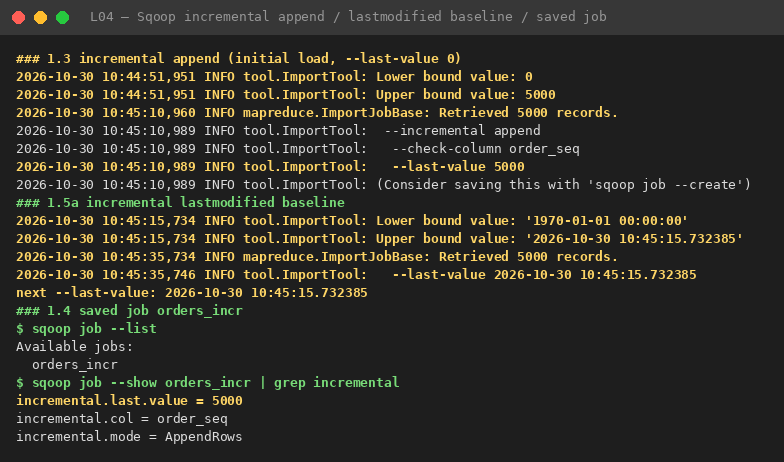
\includegraphics[keepaspectratio]{L04/img/04_sqoop_incremental_and_saved_job.png}}
\pandocbounded{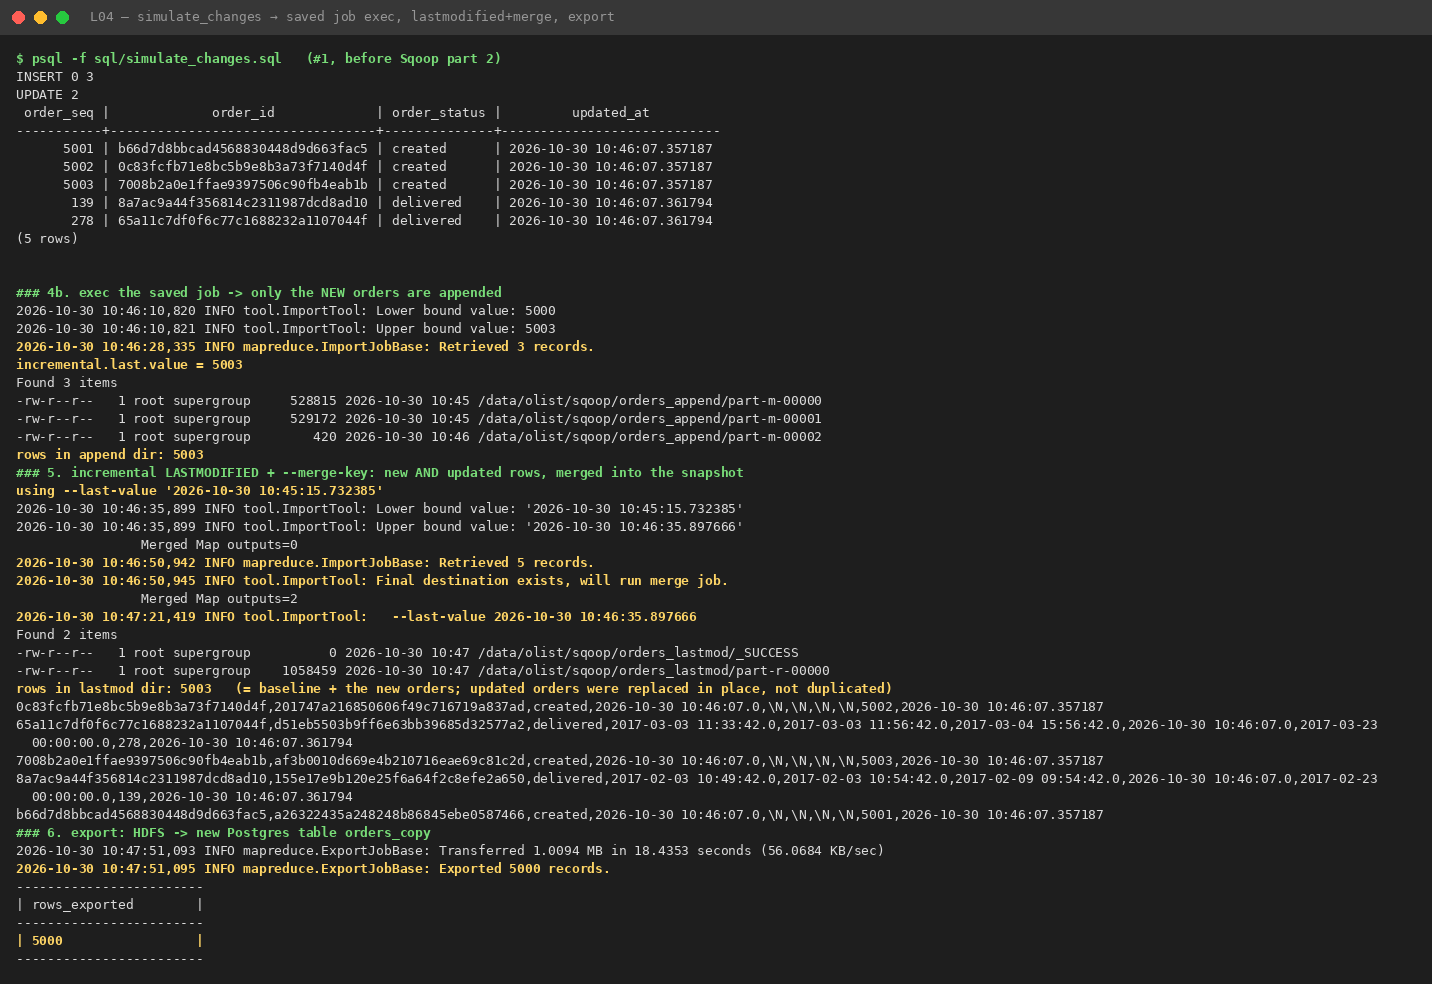
\includegraphics[keepaspectratio]{L04/img/06_sqoop_after_changes_merge_export.png}}
\pandocbounded{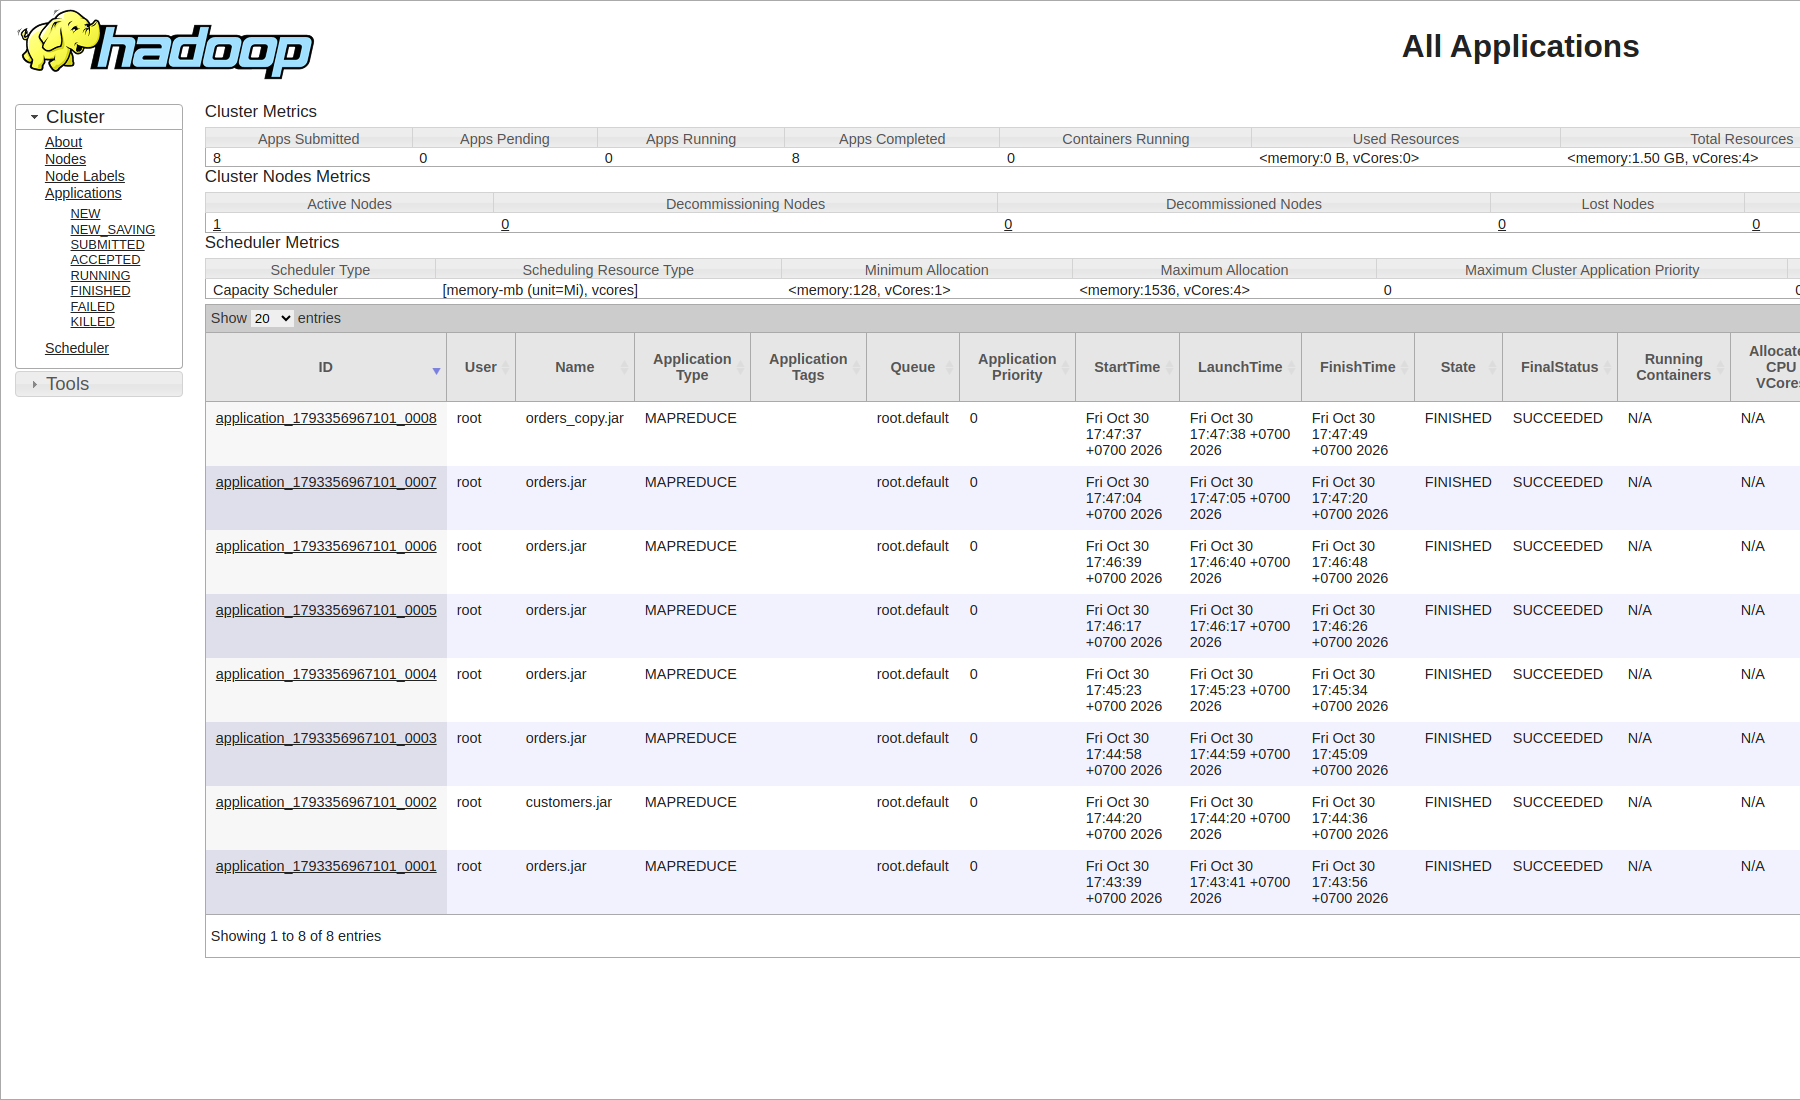
\includegraphics[keepaspectratio]{L04/img/20_ui_yarn_sqoop_jobs.png}}
\pandocbounded{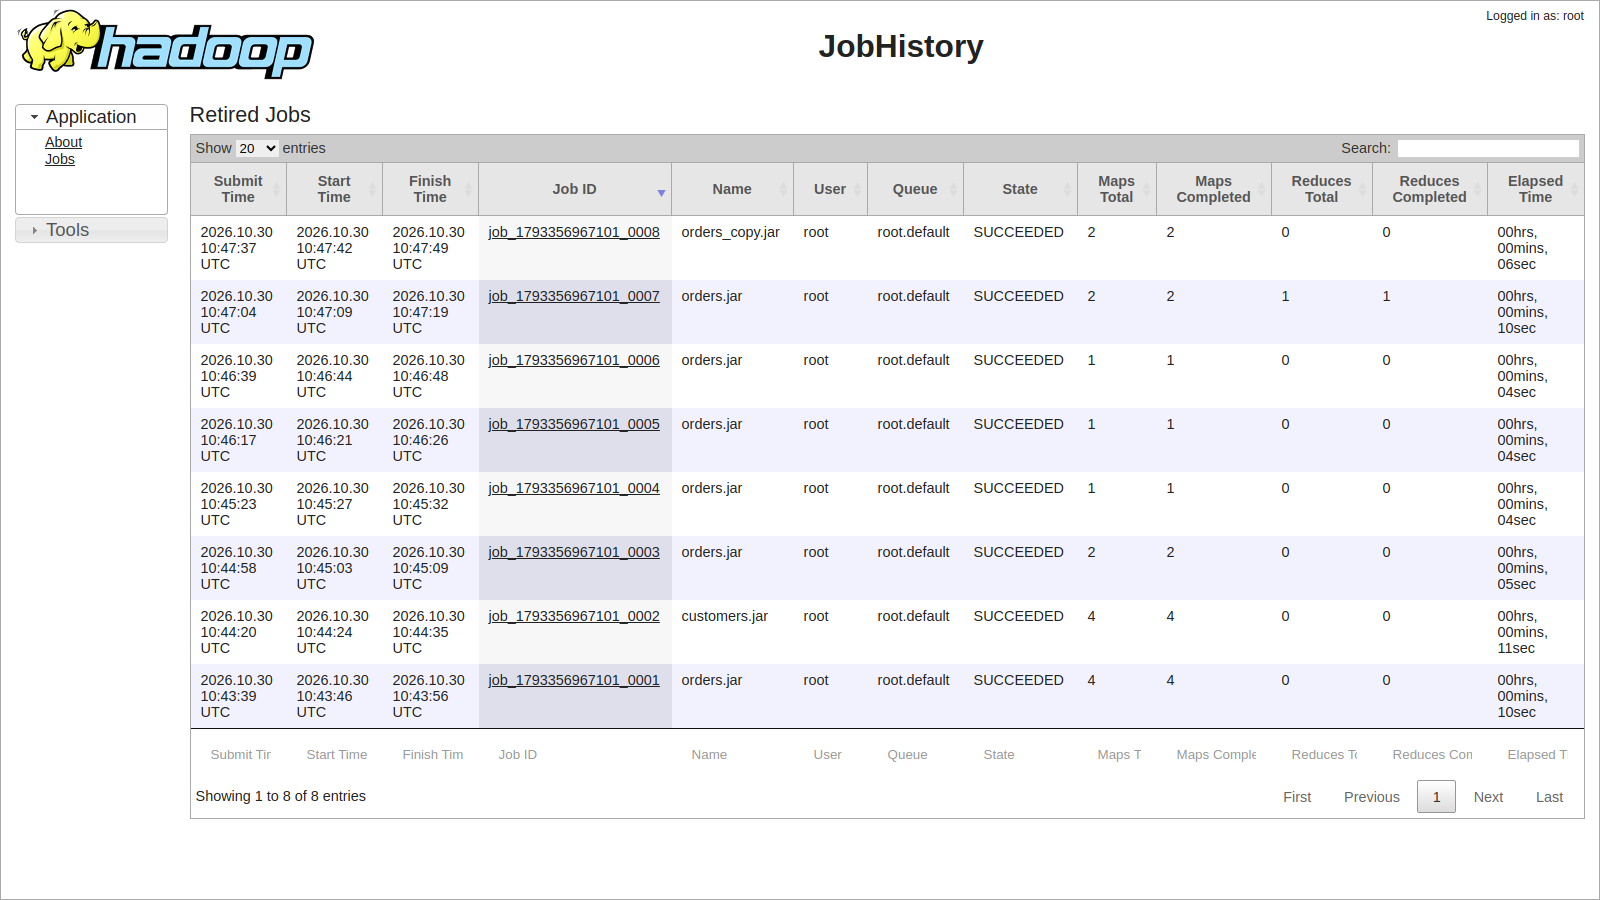
\includegraphics[keepaspectratio]{L04/img/21_ui_jobhistory_sqoop.png}}

\subsection{4. Spark JDBC: đọc song song và ghi Parquet (TODO
1--3)}\label{spark-jdbc-ux111ux1ecdc-song-song-vuxe0-ghi-parquet-todo-13}

\begin{longtable}[]{@{}
  >{\raggedright\arraybackslash}p{(\linewidth - 6\tabcolsep) * \real{0.2500}}
  >{\raggedright\arraybackslash}p{(\linewidth - 6\tabcolsep) * \real{0.2500}}
  >{\raggedright\arraybackslash}p{(\linewidth - 6\tabcolsep) * \real{0.2500}}
  >{\raggedright\arraybackslash}p{(\linewidth - 6\tabcolsep) * \real{0.2500}}@{}}
\toprule\noalign{}
\begin{minipage}[b]{\linewidth}\raggedright
Cách đọc
\end{minipage} & \begin{minipage}[b]{\linewidth}\raggedright
Số partition
\end{minipage} & \begin{minipage}[b]{\linewidth}\raggedright
Thời gian \texttt{count()}
\end{minipage} & \begin{minipage}[b]{\linewidth}\raggedright
Phân bố dòng
\end{minipage} \\
\midrule\noalign{}
\endhead
\bottomrule\noalign{}
\endlastfoot
Naive (không có \texttt{partitionColumn}) & 1 & 1.17 s & tất cả 5,003
dòng trong 1 task \\
\texttt{partitionColumn=order\_seq}, bounds 1..5003, 4 partitions & 4 &
0.22 s & 1,251 / 1,250 / 1,250 / 1,252 \\
\texttt{partitionColumn=order\_purchase\_timestamp} (2017-01-01 →
2018-09-01) & 4 & --- & 782 / 1,116 / 1,419 / 1,686 \\
\end{longtable}

\begin{itemize}
\item
  Spark tự sinh 4 câu SQL (log PostgreSQL):
  \texttt{WHERE\ "order\_seq"\ \textless{}\ 1252\ or\ "order\_seq"\ is\ null},
  \ldots{} , \texttt{WHERE\ "order\_seq"\ \textgreater{}=\ 3752}.
  Partition đầu và cuối để \textbf{hở}, nên mọi dòng ngoài bounds vẫn
  được đọc.
\item
  Split theo timestamp bị lệch vì số đơn tăng dần theo thời gian.
\item
  Ghi Parquet \texttt{partitionBy("purchase\_month")}:

  \begin{itemize}
  \tightlist
  \item
    mất 3.10 s, ra 21 thư mục tháng, đủ 5,003 dòng;
  \item
    query lọc
    \texttt{purchase\_month\ =\ \textquotesingle{}2018-08\textquotesingle{}}
    cho thấy \texttt{PartitionFilters} trong physical plan, tức là có
    partition pruning.
  \end{itemize}
\item
  Các bảng khác:

  \begin{longtable}[]{@{}ll@{}}
  \toprule\noalign{}
  Bảng & Số dòng \\
  \midrule\noalign{}
  \endhead
  \bottomrule\noalign{}
  \endlastfoot
  customers & 5,003 \\
  order\_items & 5,852 \\
  order\_payments & 5,472 \\
  products & 1,500 \\
  sellers & 312 \\
  \end{longtable}
\item
  Toàn bộ \texttt{spark-submit\ ...\ full} chạy hết 21.2 s.
\end{itemize}

\pandocbounded{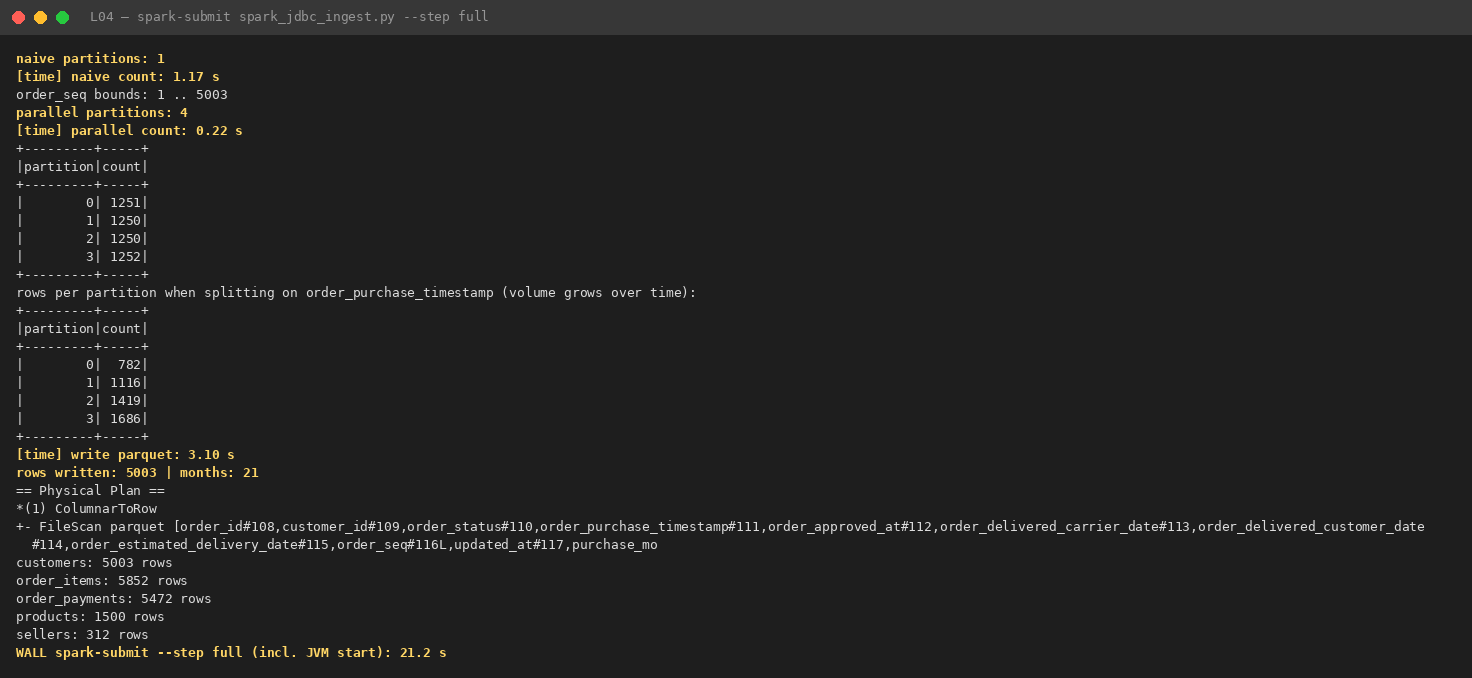
\includegraphics[keepaspectratio]{L04/img/07_spark_full.png}}
\pandocbounded{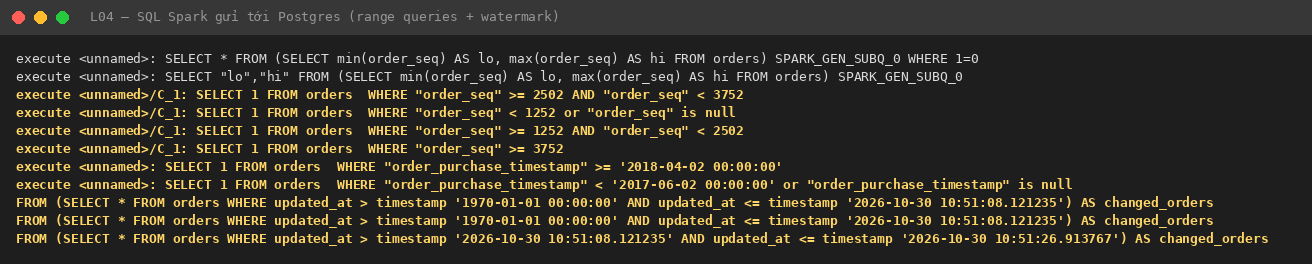
\includegraphics[keepaspectratio]{L04/img/08_postgres_log_spark_sql.png}}
\pandocbounded{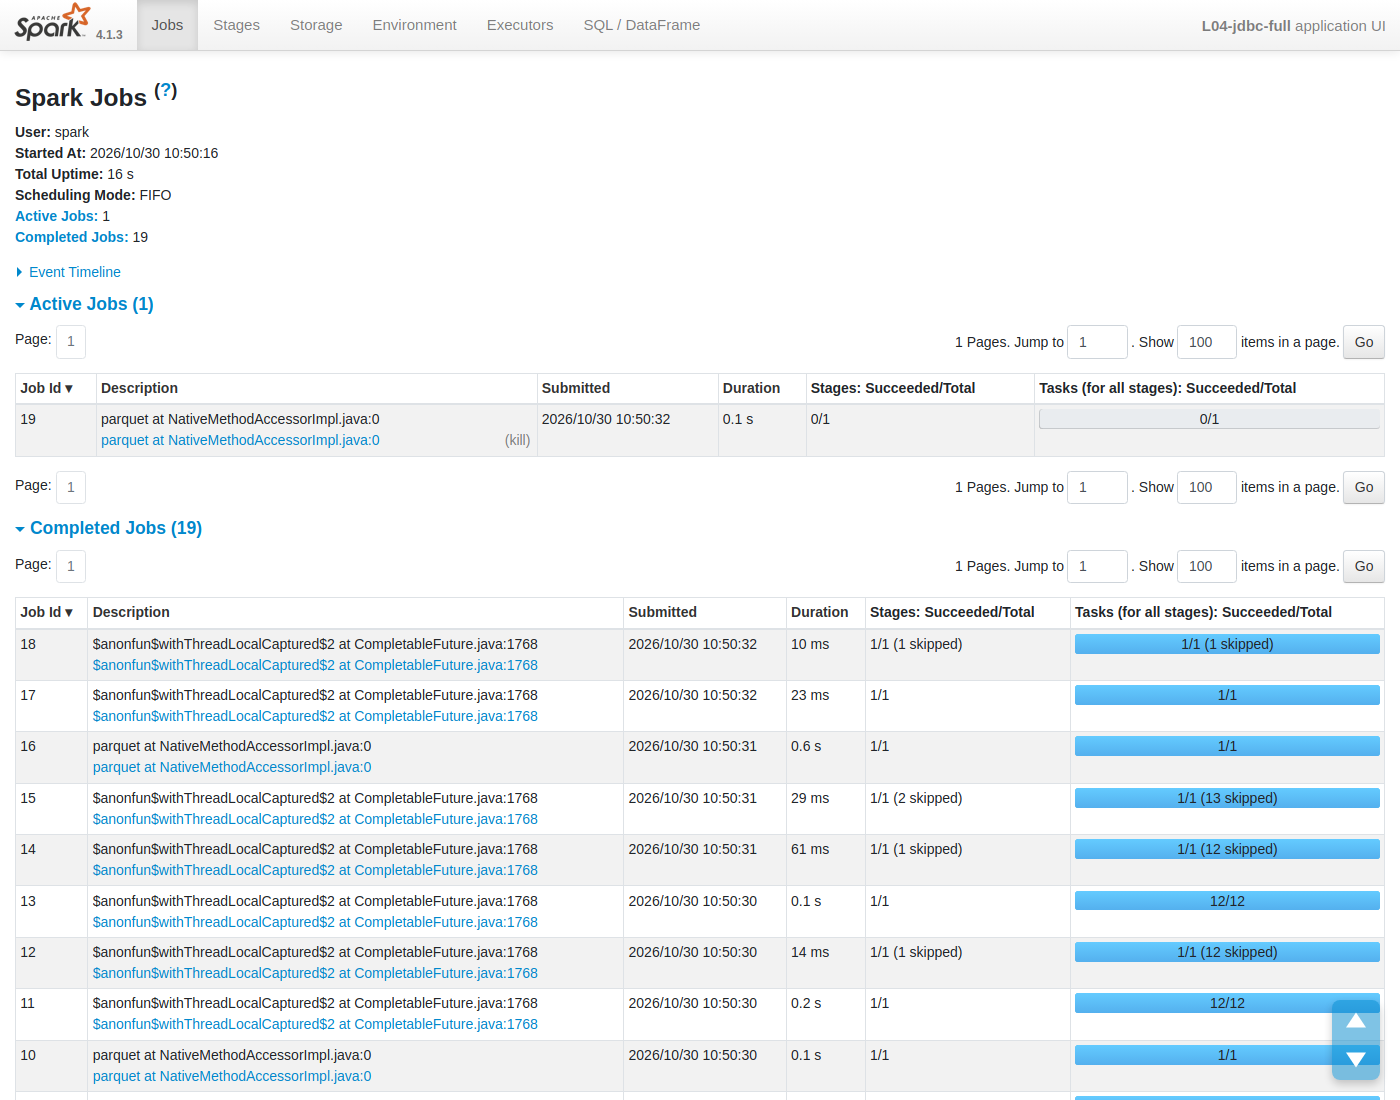
\includegraphics[keepaspectratio]{L04/img/22_ui_spark_full_jobs.png}}
\pandocbounded{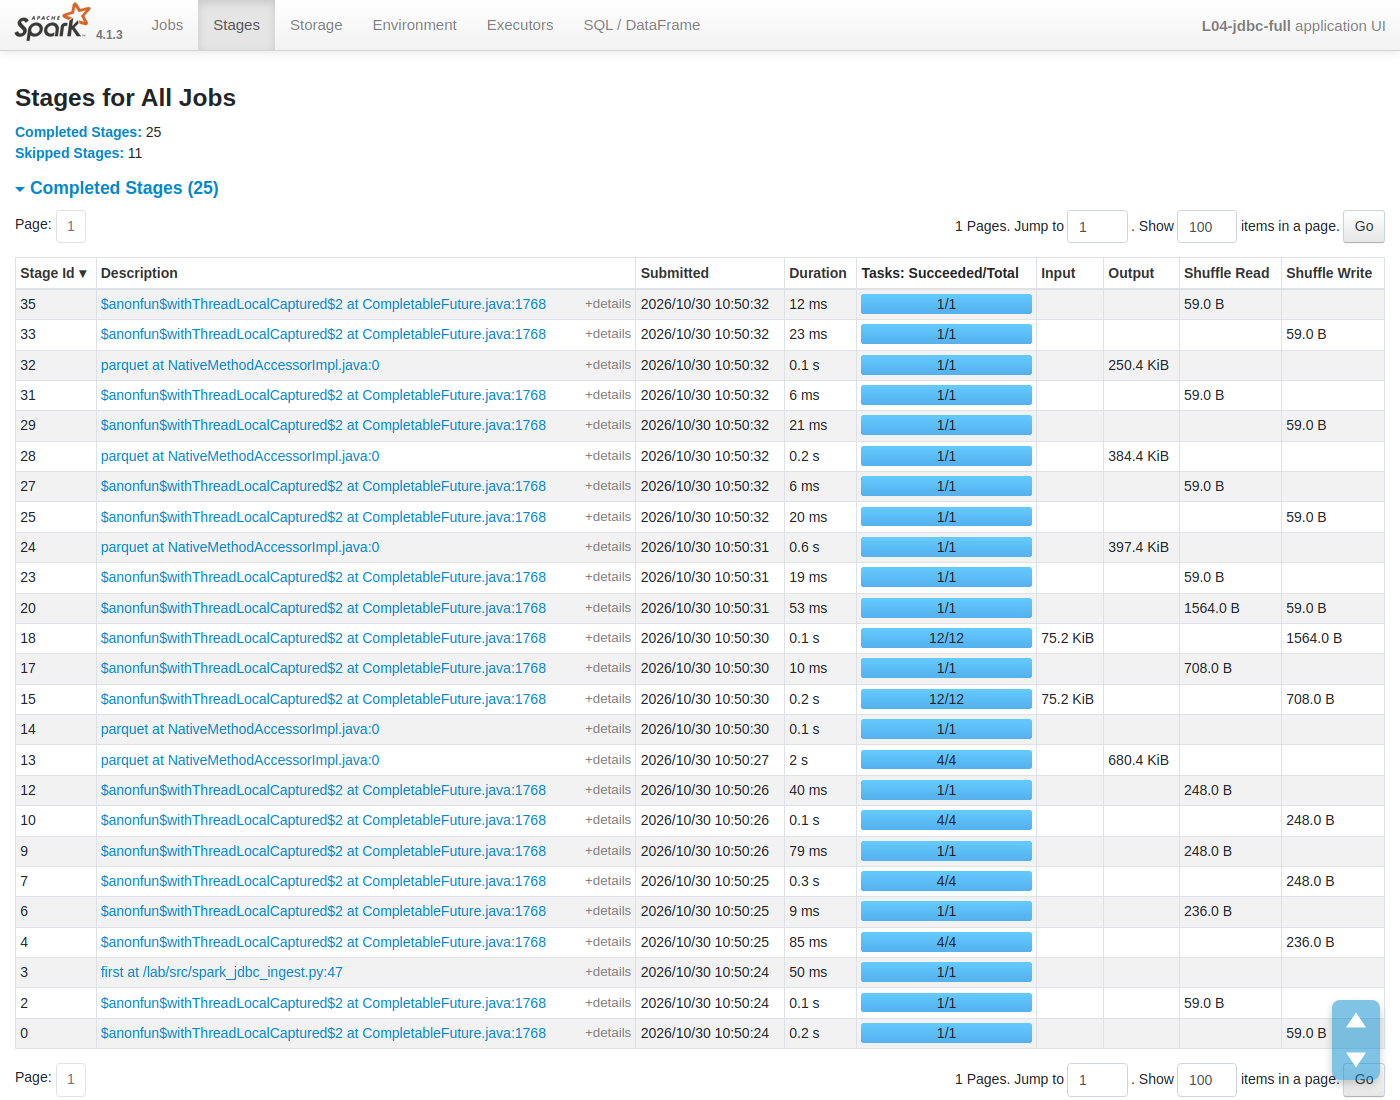
\includegraphics[keepaspectratio]{L04/img/23_ui_spark_full_stages_4tasks.png}}
\pandocbounded{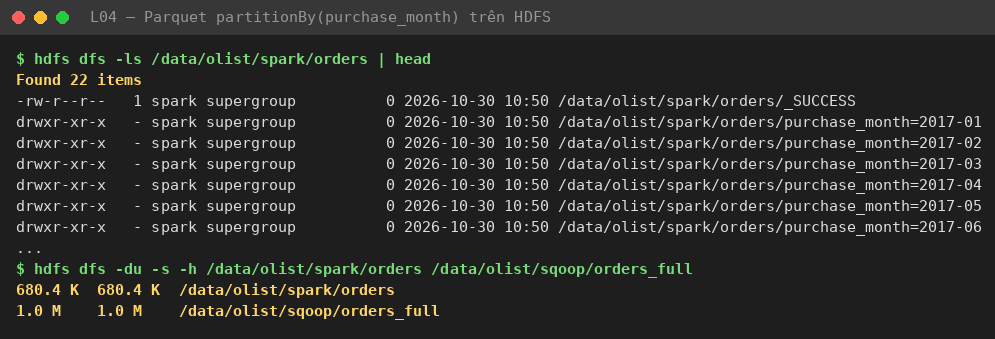
\includegraphics[keepaspectratio]{L04/img/09_spark_output_hdfs.png}}

\subsubsection{So sánh Sqoop và Spark JDBC
(orders)}\label{so-suxe1nh-sqoop-vuxe0-spark-jdbc-orders}

\begin{longtable}[]{@{}
  >{\raggedright\arraybackslash}p{(\linewidth - 4\tabcolsep) * \real{0.3333}}
  >{\raggedright\arraybackslash}p{(\linewidth - 4\tabcolsep) * \real{0.3333}}
  >{\raggedright\arraybackslash}p{(\linewidth - 4\tabcolsep) * \real{0.3333}}@{}}
\toprule\noalign{}
\begin{minipage}[b]{\linewidth}\raggedright
\end{minipage} & \begin{minipage}[b]{\linewidth}\raggedright
Sqoop (MapReduce)
\end{minipage} & \begin{minipage}[b]{\linewidth}\raggedright
Spark JDBC
\end{minipage} \\
\midrule\noalign{}
\endhead
\bottomrule\noalign{}
\endlastfoot
Song song & \texttt{-m\ 4}, chia theo MIN/MAX của \texttt{-\/-split-by}
& \texttt{numPartitions=4}, chia theo
\texttt{lowerBound}/\texttt{upperBound} do mình truyền vào \\
Thời gian & 25.2 s MR job (28.5 s cả lệnh) & 3.10 s ghi Parquet (21.2 s
cả \texttt{spark-submit} 7 bảng, tính cả khởi động JVM/YARN) \\
Định dạng ra & Text CSV, 1.0 MB & Parquet Snappy phân vùng theo tháng,
680.4 KB \\
Incremental & Có sẵn (\texttt{-\/-incremental}, saved job, merge) & Phải
tự viết: watermark, change log, dedup \\
Biến đổi trong lúc nạp & Không & Có (\texttt{withColumn},
\texttt{partitionBy}, \ldots) \\
\end{longtable}

Sqoop chậm chủ yếu vì phải khởi động một MR job riêng cho mỗi bảng.
Spark dùng chung một SparkSession cho cả 7 bảng và ghi thẳng ra định
dạng cột. Sqoop 1 cũng đã ngừng phát triển (Apache attic), nên ngày nay
thường dùng Spark JDBC hoặc CDC.

\subsection{5. Spark incremental: watermark, change log, snapshot (TODO
4--5)}\label{spark-incremental-watermark-change-log-snapshot-todo-45}

\begin{longtable}[]{@{}
  >{\raggedright\arraybackslash}p{(\linewidth - 8\tabcolsep) * \real{0.2000}}
  >{\raggedright\arraybackslash}p{(\linewidth - 8\tabcolsep) * \real{0.2000}}
  >{\raggedright\arraybackslash}p{(\linewidth - 8\tabcolsep) * \real{0.2000}}
  >{\raggedright\arraybackslash}p{(\linewidth - 8\tabcolsep) * \real{0.2000}}
  >{\raggedright\arraybackslash}p{(\linewidth - 8\tabcolsep) * \real{0.2000}}@{}}
\toprule\noalign{}
\begin{minipage}[b]{\linewidth}\raggedright
Lần chạy
\end{minipage} & \begin{minipage}[b]{\linewidth}\raggedright
Cửa sổ watermark
\end{minipage} & \begin{minipage}[b]{\linewidth}\raggedright
Dòng đọc được
\end{minipage} & \begin{minipage}[b]{\linewidth}\raggedright
Change log
\end{minipage} & \begin{minipage}[b]{\linewidth}\raggedright
Snapshot
\end{minipage} \\
\midrule\noalign{}
\endhead
\bottomrule\noalign{}
\endlastfoot
1 (lần đầu) & \texttt{(1970-01-01,\ 2026-10-30\ 10:51:08.121235{]}} &
5,003 & 5,003 & 5,003 \\
sau \texttt{simulate\_changes} \#2 (tạo 5004--5006, cập nhật 337 và 355)
& & & & \\
2 & \texttt{(10:51:08.121235,\ now{]}} & \textbf{5} & 5,008 &
\textbf{5,006} \\
3 (không có thay đổi) & \texttt{(…,\ now{]}} & \textbf{0} & 5,008 &
5,006 \\
\end{longtable}

\begin{itemize}
\tightlist
\item
  Change log chỉ append và giữ mọi phiên bản: 5,003 + 5 = 5,008.
\item
  Snapshot dùng \texttt{row\_number()} theo \texttt{order\_id}, sắp
  \texttt{updated\_at\ DESC,\ \_ingested\_at\ DESC}, nên mỗi đơn chỉ còn
  bản mới nhất: 5,006 đơn.
\item
  Lần chạy thứ ba đọc 0 dòng, nghĩa là watermark được lưu đúng và
  pipeline idempotent.
\end{itemize}

\begin{figure}
\centering
\pandocbounded{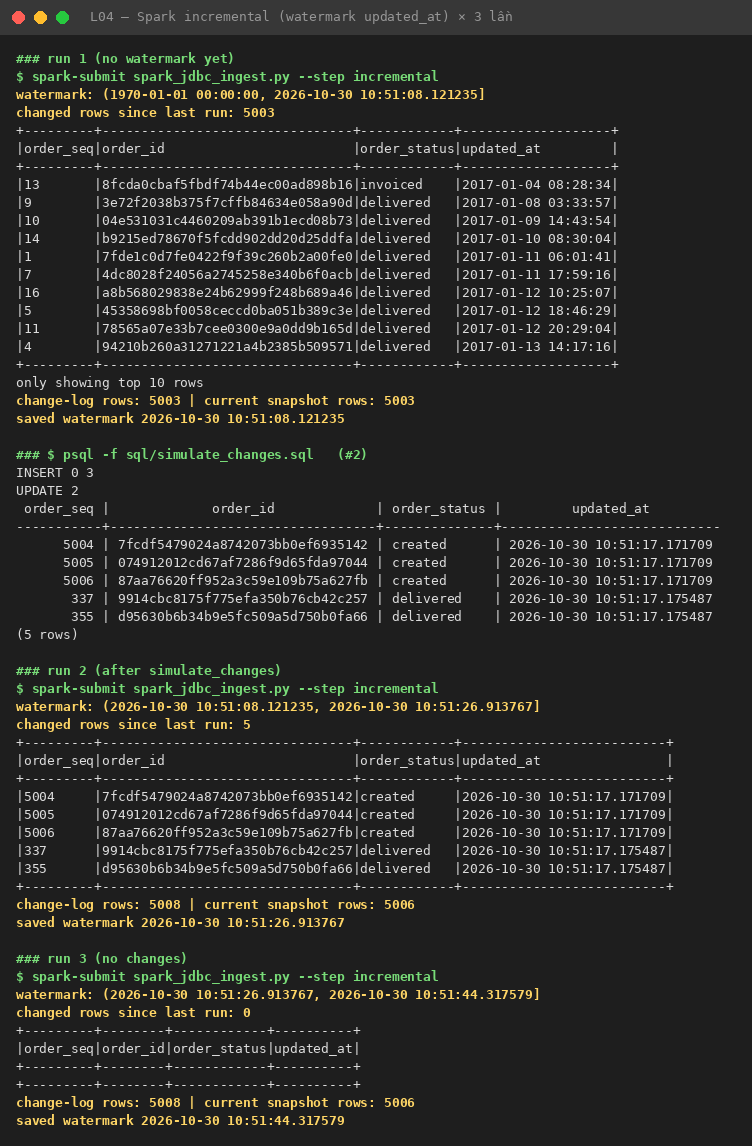
\includegraphics[keepaspectratio]{L04/img/10_spark_incremental_3runs.png}}
\caption{spark incremental}
\end{figure}

\subsection{Trả lời checkpoint}\label{trux1ea3-lux1eddi-checkpoint-3}

\textbf{Q1.} Trước khi import, Sqoop chạy bounding query
\texttt{SELECT\ MIN(order\_seq),\ MAX(order\_seq)\ FROM\ orders} (thấy
rõ trong log PostgreSQL), được (1, 5000). Nó chia khoảng này thành
\texttt{-m\ 4} đoạn \textbf{bằng nhau về giá trị}, mỗi đoạn rộng (5000 −
1)/4 ≈ 1250, và mỗi map task chạy một câu
\texttt{SELECT\ …\ WHERE\ order\_seq\ \textgreater{}=\ lo\ AND\ order\_seq\ \textless{}\ hi}.
Đoạn cuối dùng \texttt{\textless{}=} để lấy cả MAX. Vì
\texttt{order\_seq} dày đặc từ 1 đến 5000, mỗi map nhận đúng 1,250 dòng.

\textbf{Q2.} Sqoop chia theo \textbf{khoảng giá trị}, không theo số
dòng. Zip code của khách Olist tập trung ở São Paulo (01xxx--19xxx), nên
đoạn {[}1014, 24536) nhận 2,450 dòng còn đoạn {[}48057, 71578) chỉ có
427 dòng. Task chậm nhất quyết định thời gian của cả job.
\texttt{customer\_id} là chuỗi hash dạng text. Sqoop mặc định từ chối
split theo cột text và báo lỗi, trừ khi bật
\texttt{-Dorg.apache.sqoop.splitter.allow\_text\_splitter=true}. Kể cả
khi bật, việc chia theo thứ tự chuỗi vẫn kém tin cậy (phụ thuộc
collation), và split có thể lệch hoặc rỗng. Nên chọn một cột số, phân bố
đều và có index, như \texttt{order\_seq}.

\textbf{Q3.} \textbf{Có.} \texttt{lowerBound}/\texttt{upperBound} chỉ
dùng để tính \textbf{bước chia} (stride), \textbf{không phải bộ lọc}.
Spark sinh partition đầu là
\texttt{order\_seq\ \textless{}\ 1252\ OR\ order\_seq\ IS\ NULL} và
partition cuối là \texttt{order\_seq\ \textgreater{}=\ 3752}, không có
cận trên. Vì vậy dòng \texttt{order\_seq\ =\ 9,999} vẫn được đọc và rơi
vào \textbf{partition cuối}. Nếu nhiều dòng nằm ngoài bounds, partition
đầu hoặc cuối sẽ phình to và gây skew. Phải lấy bounds thật (MIN/MAX)
trước khi đọc, như script đã làm (\texttt{bounds\ 1..5003}).

\textbf{Q4.} - \textbf{Chốt cận trên trước khi đọc:}
\texttt{wm\_new\ =\ now()} được lấy \emph{trước} khi đọc, và query dùng
\texttt{updated\_at\ \textgreater{}\ wm\_old\ AND\ updated\_at\ \textless{}=\ wm\_new}.
Nếu lấy \texttt{now()} \emph{sau} khi đọc, những dòng được cập nhật
\textbf{trong lúc} đang đọc sẽ có \texttt{updated\_at} nằm trước
watermark mới mà không nằm trong dữ liệu đã đọc. Lần chạy sau sẽ bỏ qua
chúng vĩnh viễn: \textbf{mất dữ liệu}. Cận trên cố định cũng giúp các
partition JDBC song song nhìn cùng một cửa sổ, và lần sau bắt đầu đúng
từ chỗ lần này dừng. - \textbf{Chỉ lưu watermark sau khi ghi thành
công:} nếu job chết giữa chừng, watermark cũ vẫn còn và lần chạy lại sẽ
đọc lại cả cửa sổ. Như vậy dữ liệu được giao \textbf{at-least-once}: có
thể trùng nhưng không mất. Phần trùng được dedup idempotent bằng
\texttt{row\_number()} theo \texttt{order\_id} khi dựng snapshot. Nếu
lưu watermark trước khi ghi mà ghi thất bại, cửa sổ đó sẽ bị bỏ qua mãi
mãi.

\textbf{Q5.} \texttt{append} chỉ dựa vào
\texttt{order\_seq\ \textgreater{}\ last\_value}, nên chỉ bắt được
\textbf{INSERT} (lần chạy job chỉ lấy 3 dòng mới). \texttt{lastmodified}
dựa vào \texttt{updated\_at\ \textgreater{}\ last\_value}, nên bắt được
cả \textbf{INSERT và UPDATE} (lấy 5 dòng: 3 mới + 2 đơn 139 và 278). Cần
\texttt{-\/-merge-key} để gộp bản cũ với bản mới. \textbf{Không chế độ
nào bắt được DELETE}: dòng đã xoá thì không còn trong bảng để query ra.

\textbf{Q6.} Watermark trên \texttt{updated\_at} \textbf{không} giải
quyết được: 1. \textbf{DELETE}: dòng bị xoá không bao giờ xuất hiện
trong query, nên bản sao trên HDFS giữ dữ liệu ``ma'' (trừ khi ứng dụng
dùng soft delete). 2. \textbf{Các lần UPDATE trung gian}: nếu một dòng
đổi nhiều lần giữa hai lần chạy (ví dụ \texttt{shipped} →
\texttt{delivered} → \texttt{canceled}), ta chỉ thấy trạng thái cuối và
mất lịch sử. 3. \textbf{\texttt{updated\_at} không đáng tin}: - ứng dụng
quên cập nhật cột, hoặc ghi bằng giờ của app server lệch đồng hồ; -
transaction dài commit \emph{sau} khi watermark đã vượt qua timestamp
của nó, nên dòng bị bỏ sót. 4. \textbf{Tải lên nguồn}: mỗi lần chạy là
một query quét theo \texttt{updated\_at} (cần index), độ trễ bằng chu kỳ
poll.

\textbf{CDC} (Debezium, L08) không query bảng mà đọc \textbf{transaction
log (WAL)} của PostgreSQL qua logical replication. Mọi INSERT, UPDATE và
DELETE được phát ra thành event theo đúng thứ tự commit, kèm ảnh trước
và sau. Không phụ thuộc cột \texttt{updated\_at}, gần như không tạo tải
query, và độ trễ chỉ vài giây.

\textbf{Q7.} \texttt{-m\ 50} hoặc \texttt{numPartitions=50} mở
\textbf{50 kết nối đồng thời}, mỗi kết nối chạy một range scan. Như vậy
dễ vượt \texttt{max\_connections} (PostgreSQL mặc định 100), làm ứng
dụng production không lấy được kết nối. Nó cũng tranh CPU, I/O và buffer
cache với tải OLTP, và với bảng nhỏ (5,000 dòng) thì mỗi task chỉ có
\textasciitilde100 dòng, chi phí khởi tạo lấn át lợi ích. Thực tế nên
giới hạn khoảng 4--8 kết nối, đọc từ \textbf{read replica} hoặc ngoài
giờ cao điểm, và đặt \texttt{fetchsize} hợp lý.

\newpage

\section{L05 --- PySpark cơ bản: DataFrame, Spark SQL và Spark
UI}\label{l05-pyspark-cux1a1-bux1ea3n-dataframe-spark-sql-vuxe0-spark-ui}

Môi trường: Spark \textbf{4.1.3} (image \texttt{spark:4.1.3-python3},
Java 17, Python 3.10), \texttt{local{[}4{]}}, driver 2 GB,
\texttt{spark.sql.shuffle.partitions=8}. Dữ liệu:
\texttt{yellow\_tripdata\_2024-01.parquet} (2,964,624 dòng) và
\texttt{taxi\_zone\_lookup.csv}.

Log gốc:

\begin{longtable}[]{@{}
  >{\raggedright\arraybackslash}p{(\linewidth - 2\tabcolsep) * \real{0.5000}}
  >{\raggedright\arraybackslash}p{(\linewidth - 2\tabcolsep) * \real{0.5000}}@{}}
\toprule\noalign{}
\begin{minipage}[b]{\linewidth}\raggedright
File
\end{minipage} & \begin{minipage}[b]{\linewidth}\raggedright
Nội dung
\end{minipage} \\
\midrule\noalign{}
\endhead
\bottomrule\noalign{}
\endlastfoot
\texttt{01\_run\_no\_repartition.txt} & lần chạy ghi \textbf{không}
\texttt{repartition} \\
\texttt{03\_run\_with\_repartition.txt} & lần chạy chính, có
\texttt{repartition} và \texttt{-\/-hold\ 300} để chụp UI \\
\texttt{02\_files\_no\_repartition.txt},
\texttt{04\_files\_with\_repartition.txt} & đếm file output \\
\texttt{05\_ansi\_divide\_by\_zero.txt} & demo ANSI mode \\
\end{longtable}

\subsection{File nộp}\label{file-nux1ed9p-2}

\texttt{l05\_basics.py}: đã hoàn thành TODO 1--7. Thêm cờ
\texttt{-\/-no-repartition} để chạy thí nghiệm TODO 7 mà không phải sửa
code.

\begin{figure}
\centering
\pandocbounded{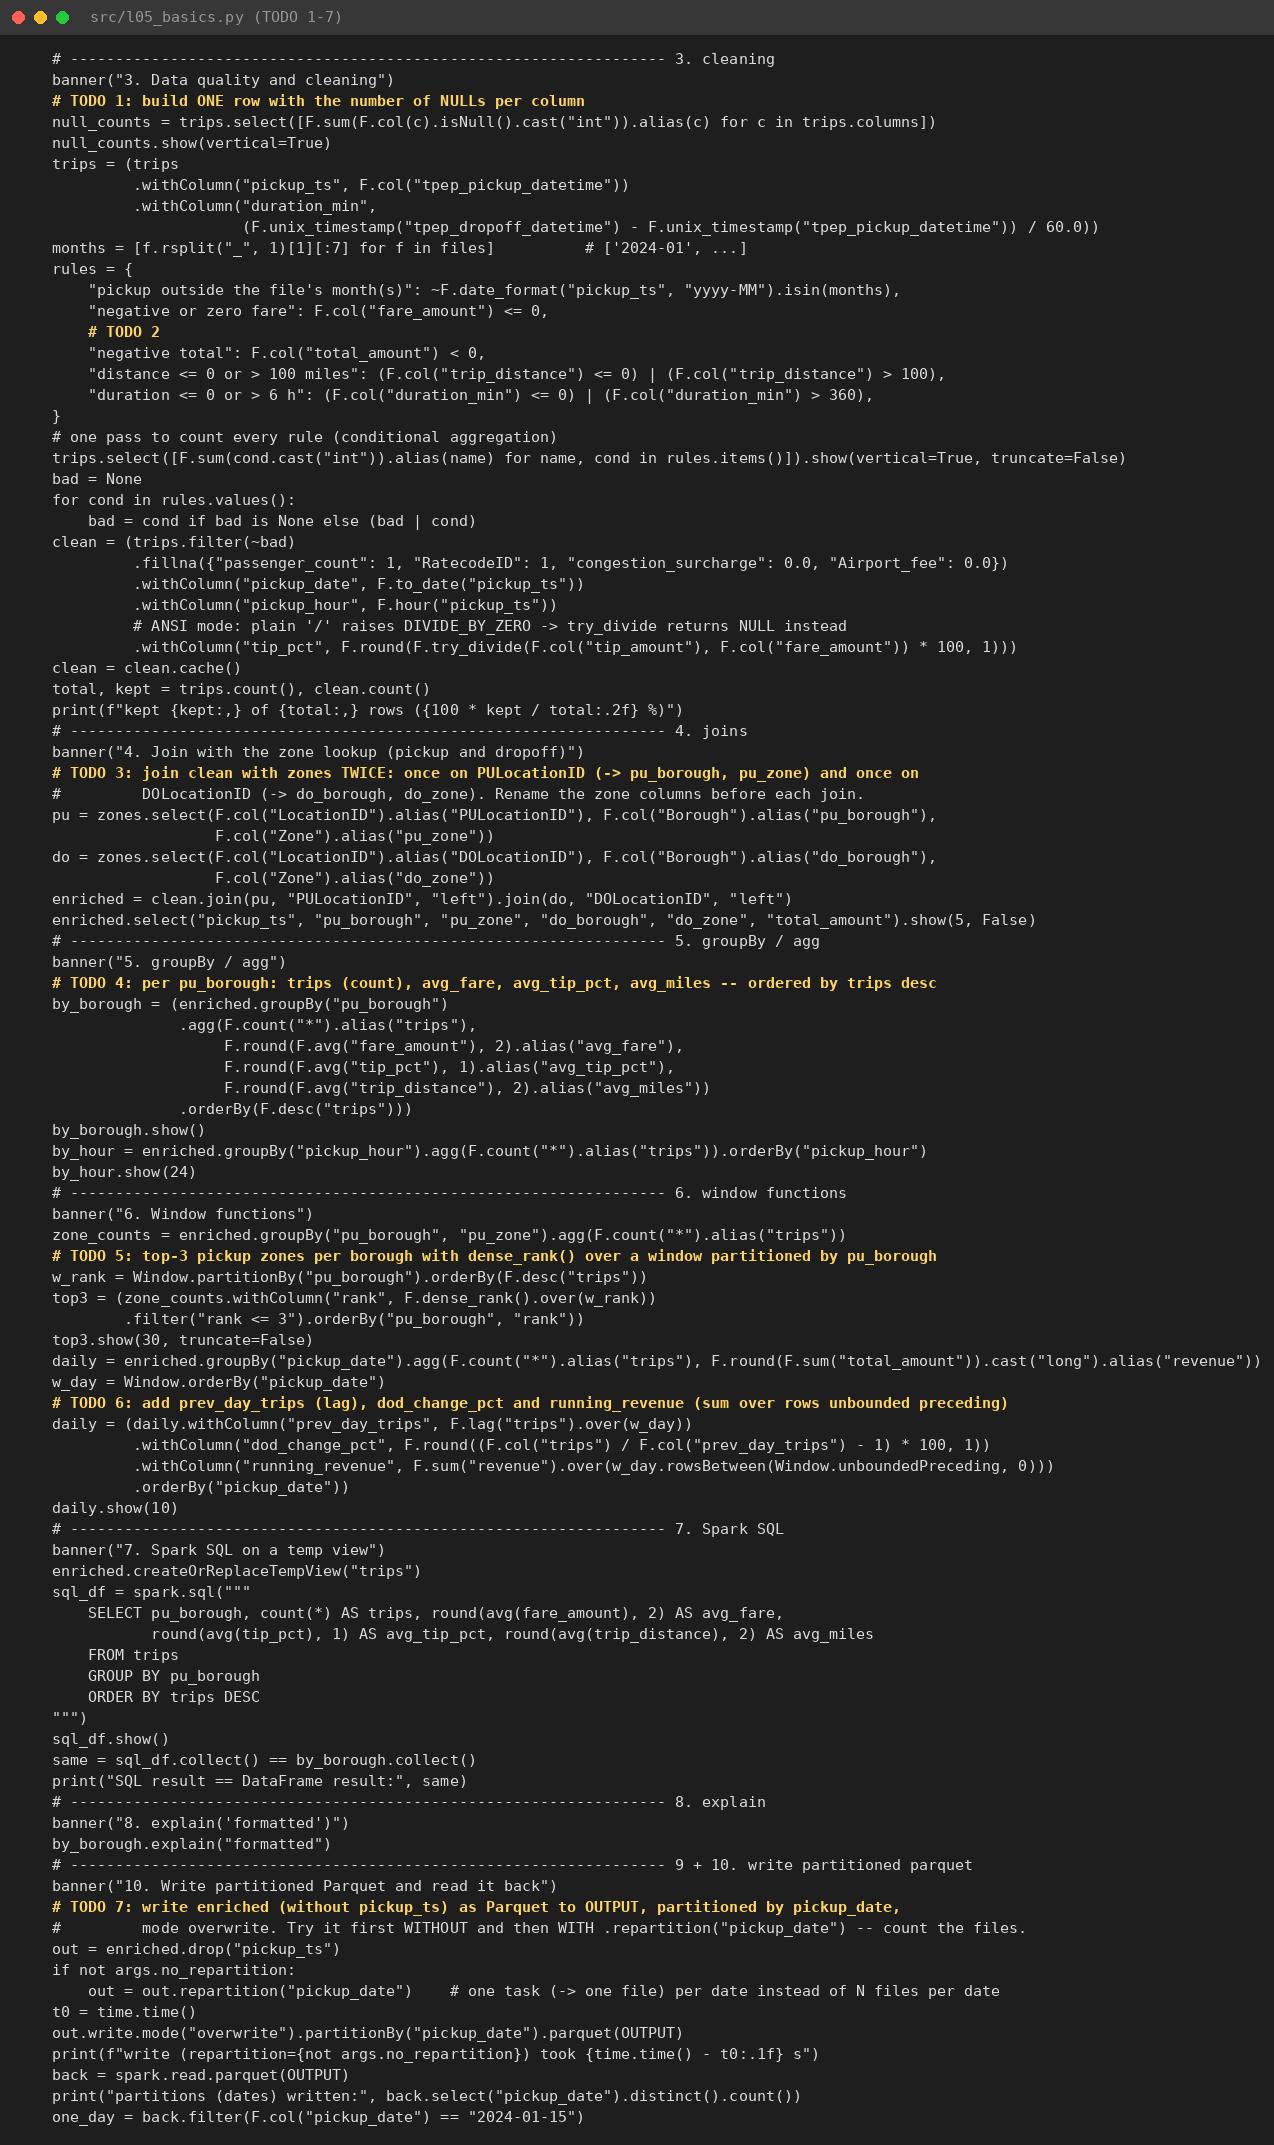
\includegraphics[keepaspectratio]{L05/img/code_l05_basics.png}}
\caption{code}
\end{figure}

\subsection{Kết quả chính (khớp đáp
án)}\label{kux1ebft-quux1ea3-chuxednh-khux1edbp-ux111uxe1p-uxe1n}

\begin{longtable}[]{@{}
  >{\raggedright\arraybackslash}p{(\linewidth - 2\tabcolsep) * \real{0.5000}}
  >{\raggedright\arraybackslash}p{(\linewidth - 2\tabcolsep) * \real{0.5000}}@{}}
\toprule\noalign{}
\begin{minipage}[b]{\linewidth}\raggedright
Hạng mục
\end{minipage} & \begin{minipage}[b]{\linewidth}\raggedright
Kết quả
\end{minipage} \\
\midrule\noalign{}
\endhead
\bottomrule\noalign{}
\endlastfoot
Số dòng / số partition đầu vào & 2,964,624 / 4 \\
3 transformation (filter, withColumn, select) & \textbf{0.096 s}, chưa
có job nào \\
\texttt{count()} (action) & 228,254 chuyến \textgreater{} 10 dặm, 0.28
s \\
NULL ở 5 cột \texttt{passenger\_count}, \texttt{RatecodeID},
\texttt{store\_and\_fwd\_flag}, \texttt{congestion\_surcharge},
\texttt{Airport\_fee} & \textbf{140,162} mỗi cột \\
Luật làm sạch & ngoài tháng 18 · fare ≤ 0: 38,341 · total \textless{} 0:
35,504 · distance: 60,430 · duration: 2,642 \\
Giữ lại sau làm sạch & \textbf{2,867,786 / 2,964,624 (96.73 \%)} \\
Manhattan & 2,571,810 chuyến, fare 14.92, tip 21.6 \%, 2.31 dặm \\
Queens & 257,573 chuyến, fare 52.77, 12.76 dặm (sân bay) \\
Giờ đông nhất & 18:00 (206,163 chuyến) \\
Top-3 Manhattan & Midtown Center 140,065 · UES South 140,059 · UES North
133,891 \\
Top-3 Queens & JFK 138,296 · LaGuardia 87,657 · East Elmhurst 11,861 \\
SQL so với DataFrame &
\texttt{SQL\ result\ ==\ DataFrame\ result:\ True} \\
Ghi Parquet phân vùng theo ngày & 31 partition, 73 MB, 8.2 s \\
Đọc lại ngày 2024-01-15 & 74,743 chuyến, có \texttt{PartitionFilters} \\
\end{longtable}

\pandocbounded{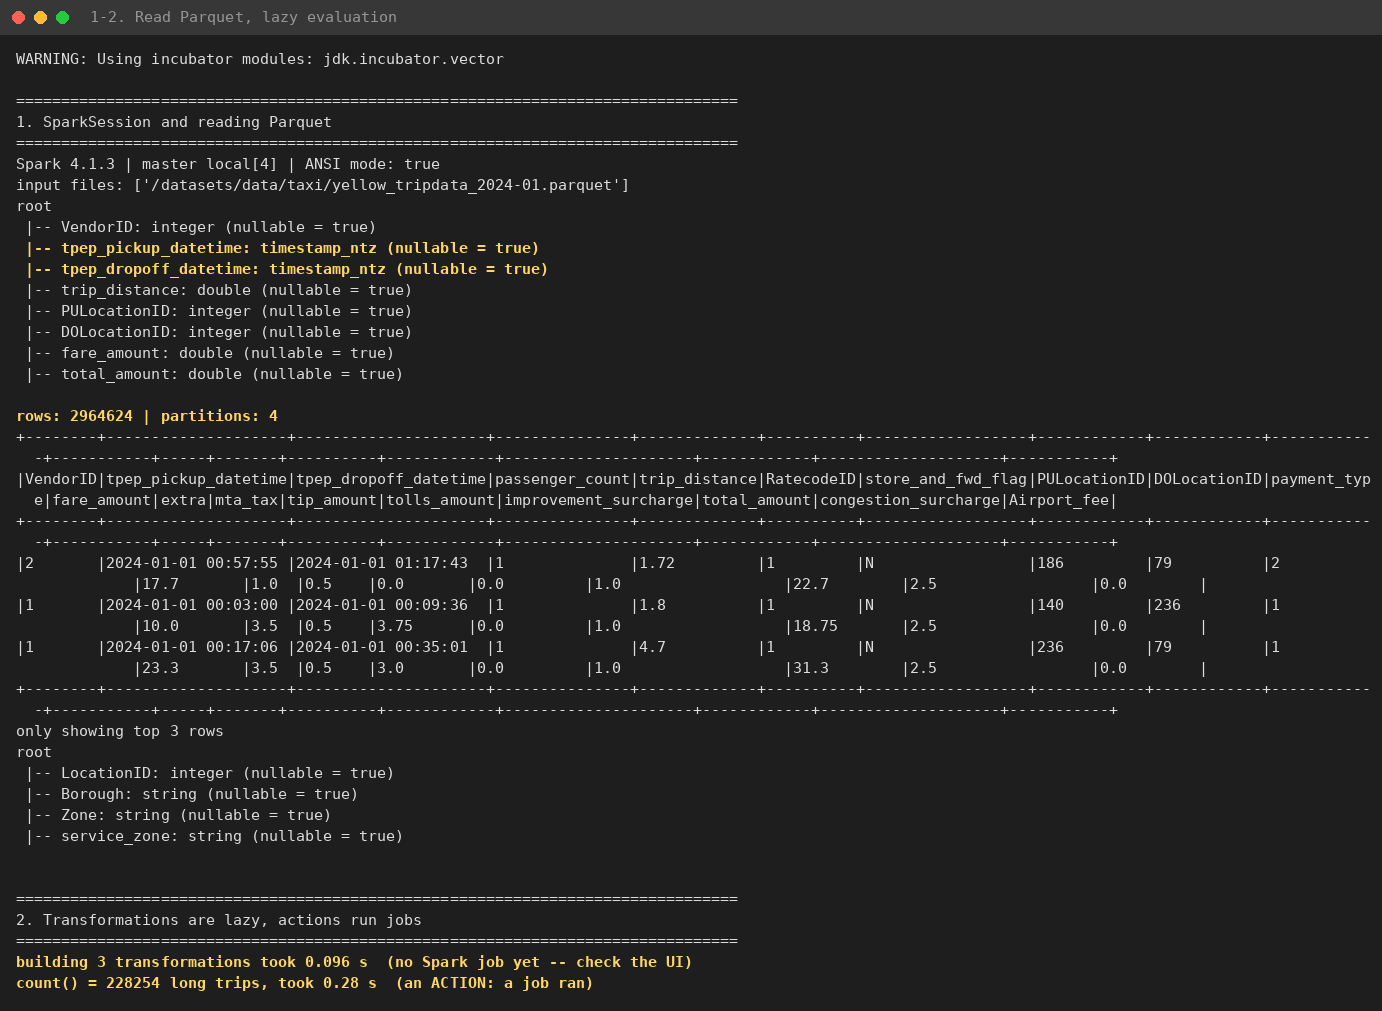
\includegraphics[keepaspectratio]{L05/img/01_read_schema_lazy.png}}
\pandocbounded{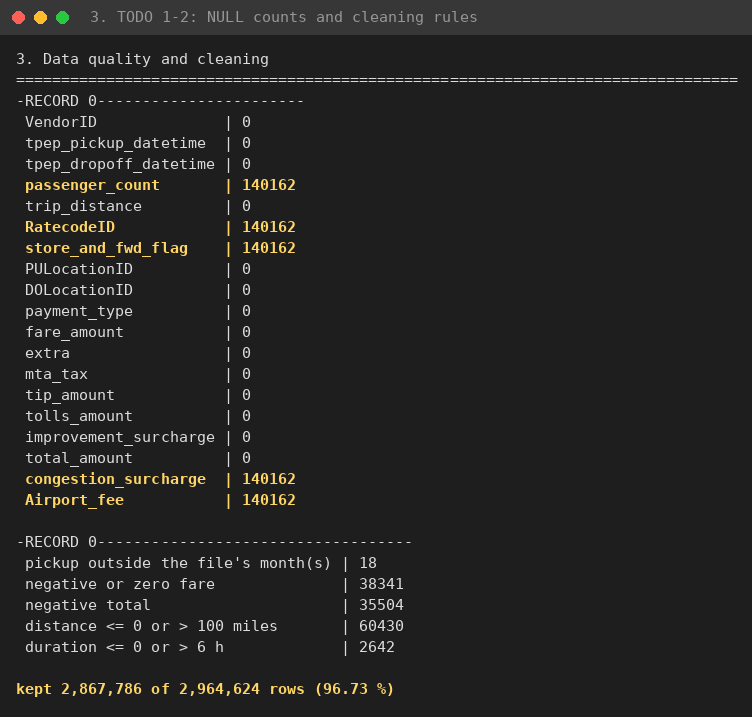
\includegraphics[keepaspectratio]{L05/img/02_cleaning_nulls_rules.png}}
\pandocbounded{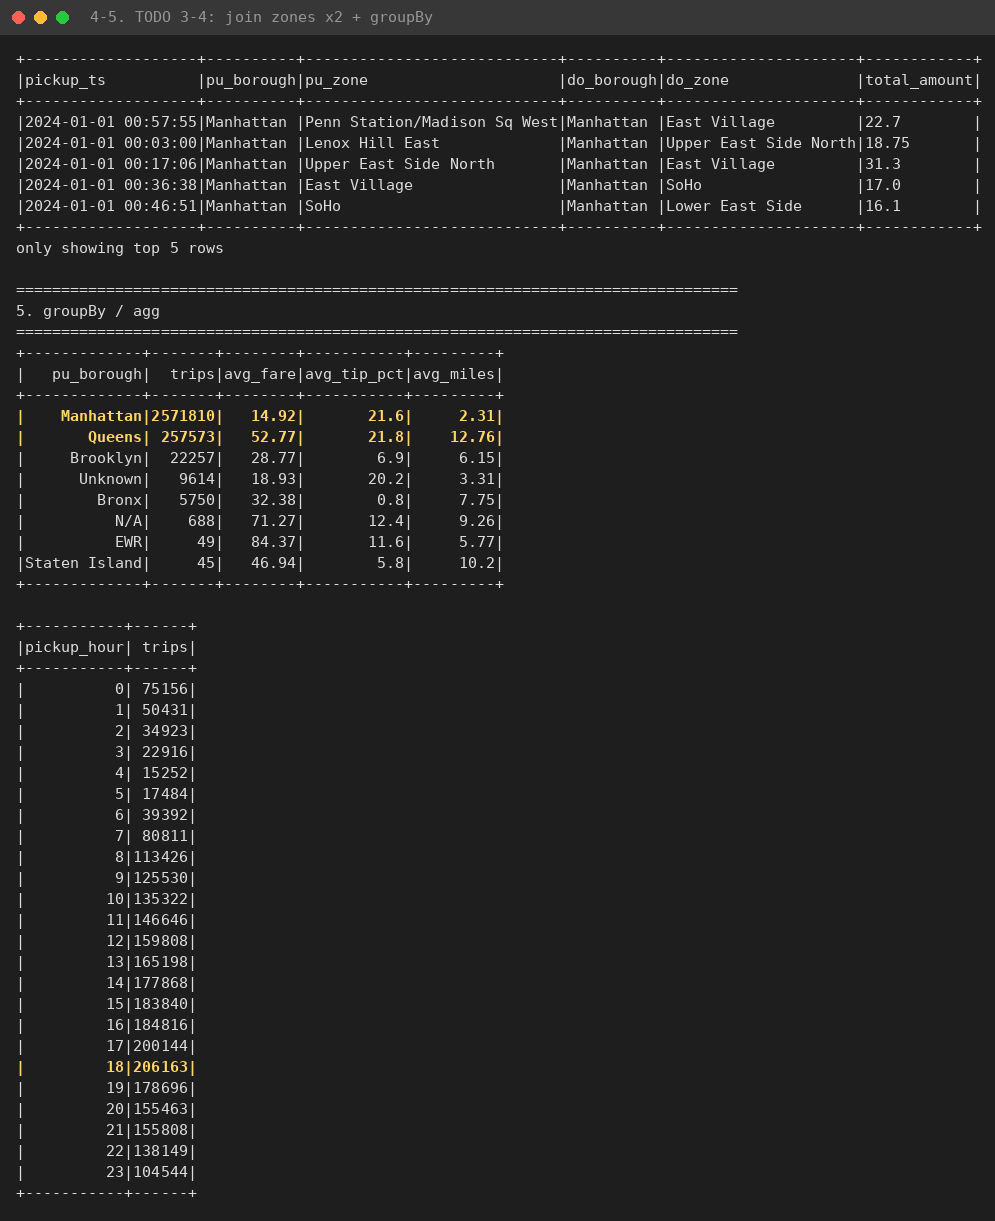
\includegraphics[keepaspectratio]{L05/img/03_join_groupby.png}}
\pandocbounded{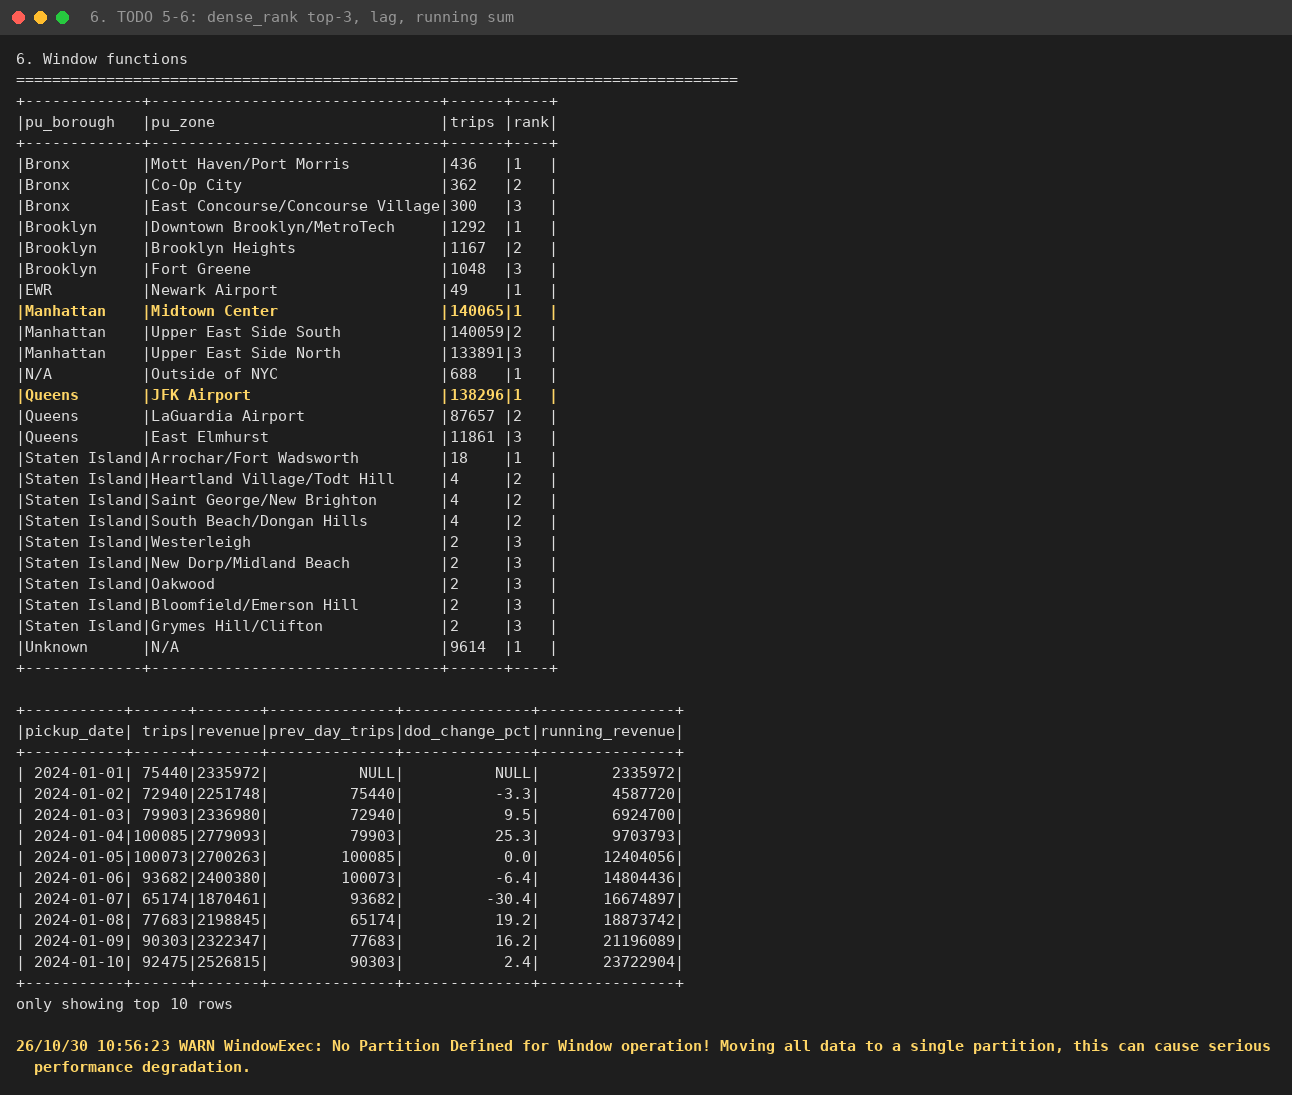
\includegraphics[keepaspectratio]{L05/img/04_window_functions.png}}

Spark 4 bật \textbf{ANSI mode} mặc định: \texttt{1/0} báo lỗi
\texttt{{[}DIVIDE\_BY\_ZERO{]}} thay vì trả NULL. Vì vậy script tính
\texttt{tip\_pct} bằng \texttt{F.try\_divide}.

\begin{figure}
\centering
\pandocbounded{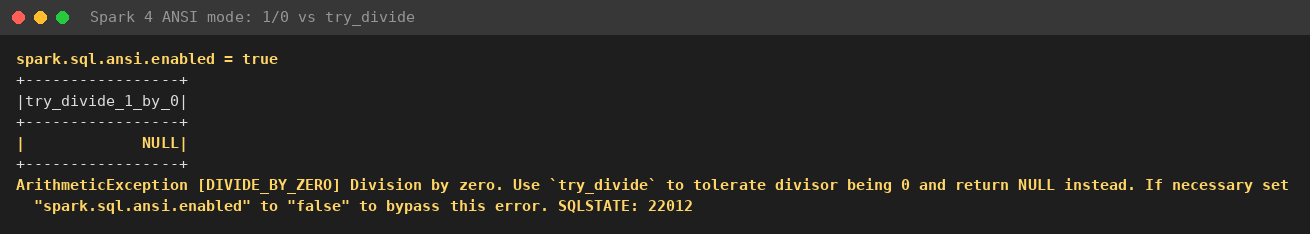
\includegraphics[keepaspectratio]{L05/img/08_ansi_divide_by_zero.png}}
\caption{ansi}
\end{figure}

\subsection{Plan và Spark UI}\label{plan-vuxe0-spark-ui}

\pandocbounded{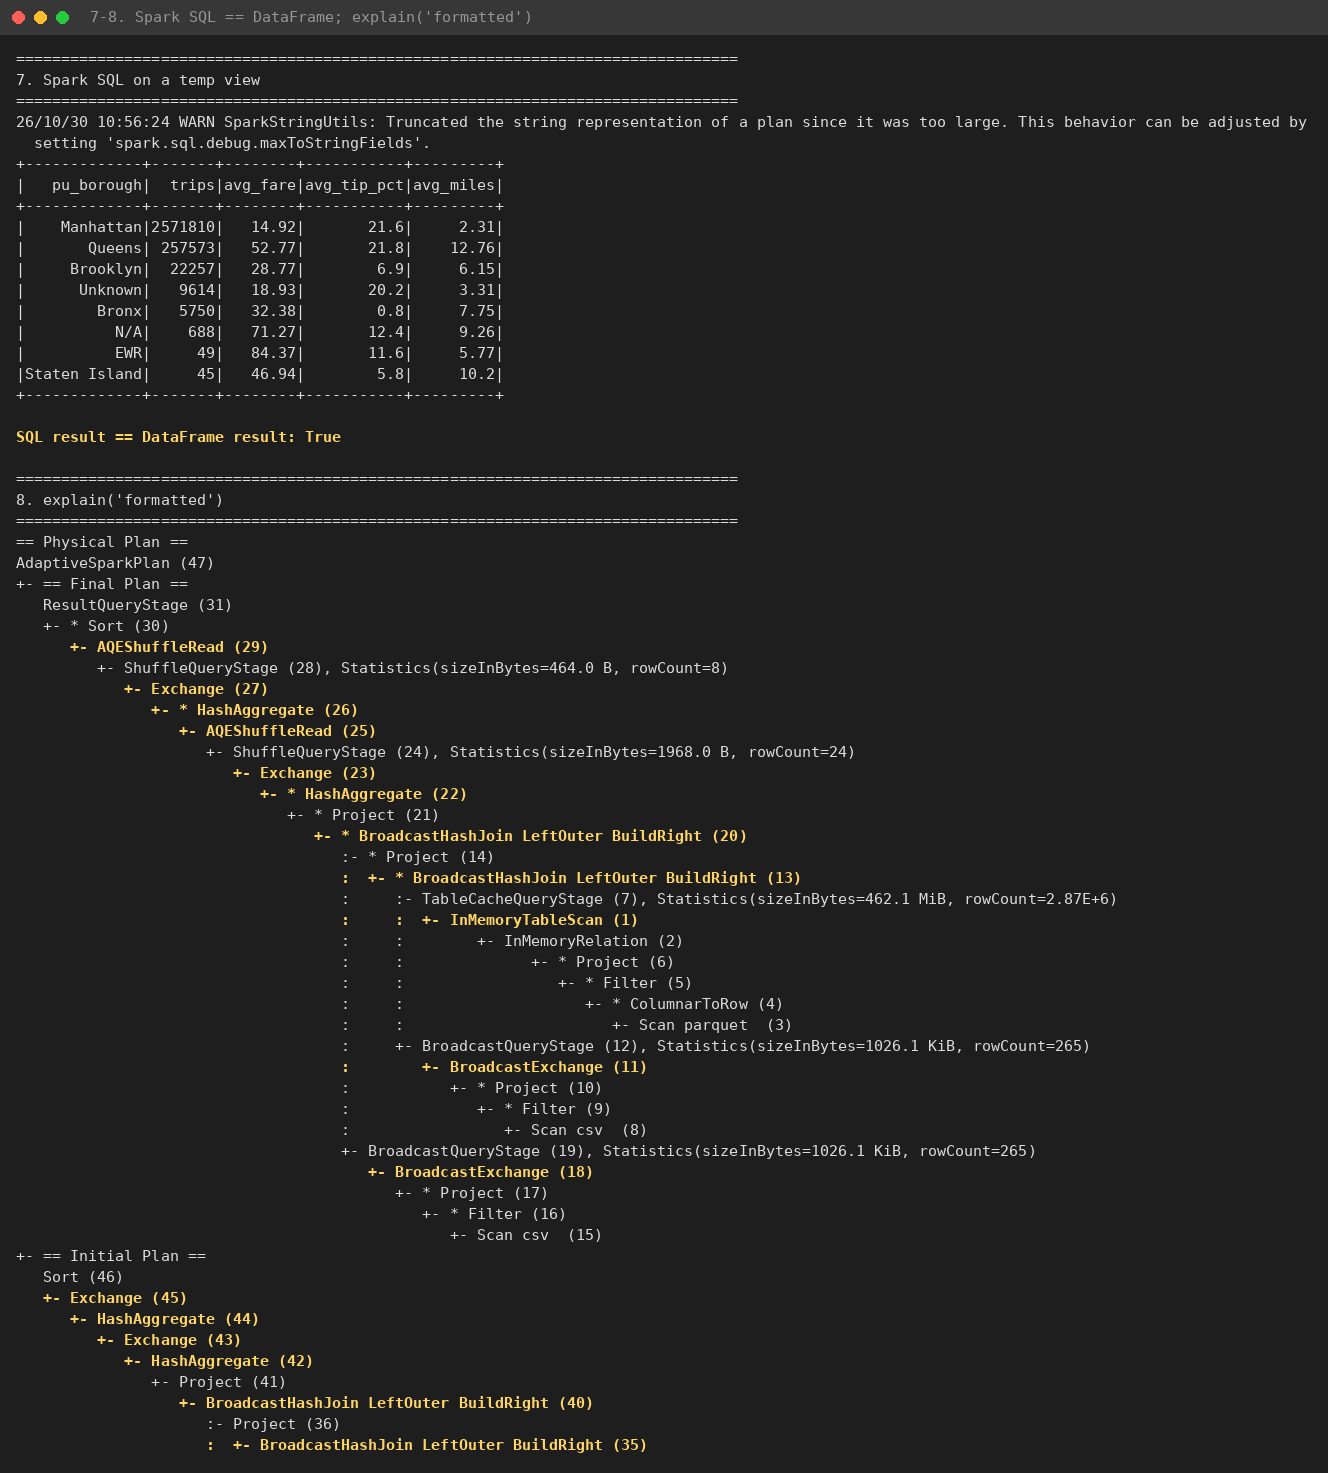
\includegraphics[keepaspectratio]{L05/img/05_sql_and_plan_tree.png}}
\pandocbounded{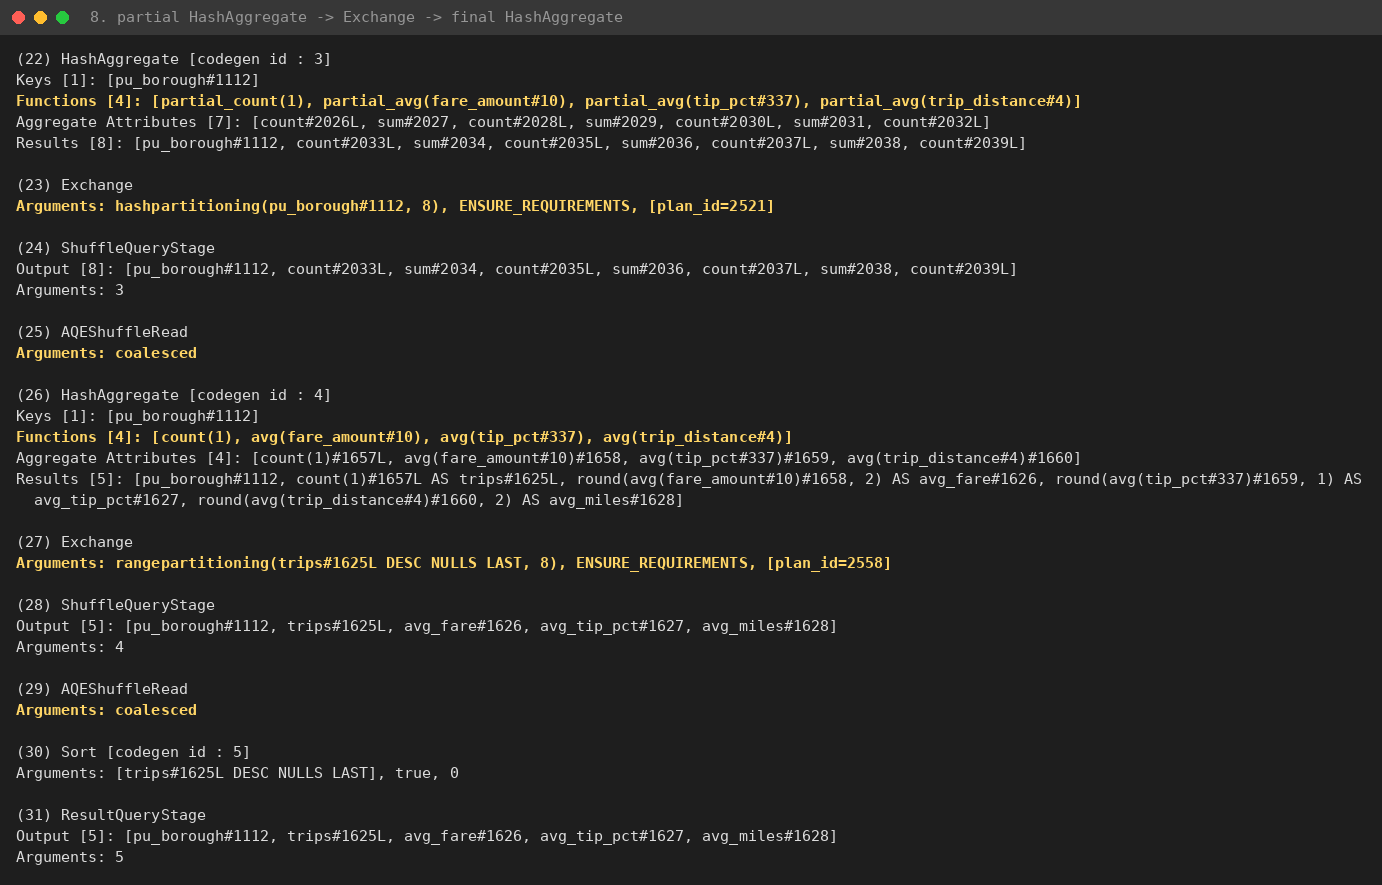
\includegraphics[keepaspectratio]{L05/img/06_plan_partial_final_agg.png}}

\begin{longtable}[]{@{}
  >{\raggedright\arraybackslash}p{(\linewidth - 4\tabcolsep) * \real{0.3333}}
  >{\raggedright\arraybackslash}p{(\linewidth - 4\tabcolsep) * \real{0.3333}}
  >{\raggedright\arraybackslash}p{(\linewidth - 4\tabcolsep) * \real{0.3333}}@{}}
\toprule\noalign{}
\begin{minipage}[b]{\linewidth}\raggedright
Tab
\end{minipage} & \begin{minipage}[b]{\linewidth}\raggedright
Ảnh
\end{minipage} & \begin{minipage}[b]{\linewidth}\raggedright
Nhận xét
\end{minipage} \\
\midrule\noalign{}
\endhead
\bottomrule\noalign{}
\endlastfoot
Jobs &
\pandocbounded{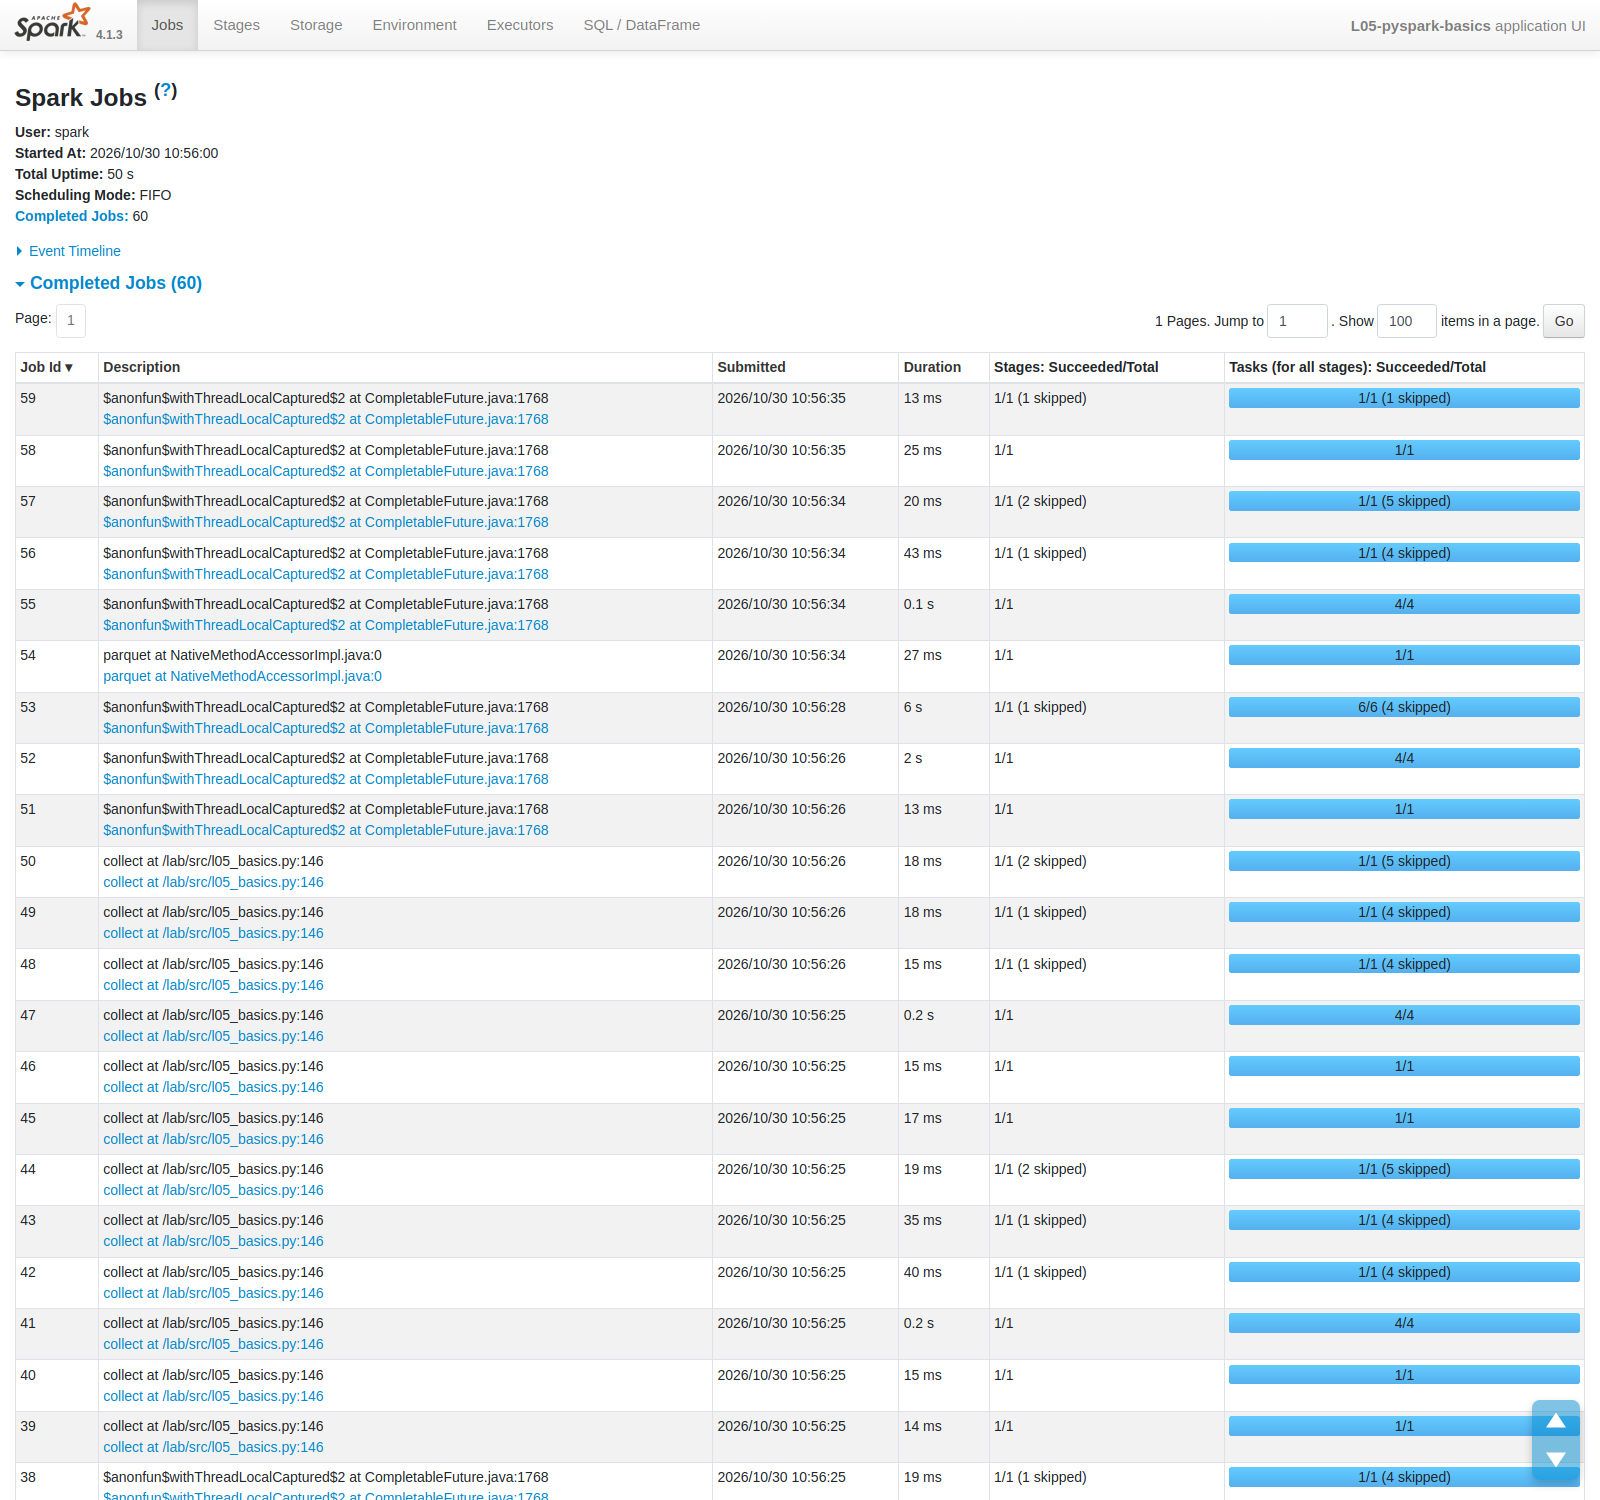
\includegraphics[keepaspectratio]{L05/img/20_ui_jobs.png}}
& mỗi action (\texttt{count}, \texttt{showString}, \texttt{collect},
\texttt{parquet}) sinh ra một hoặc nhiều job \\
Stages &
\pandocbounded{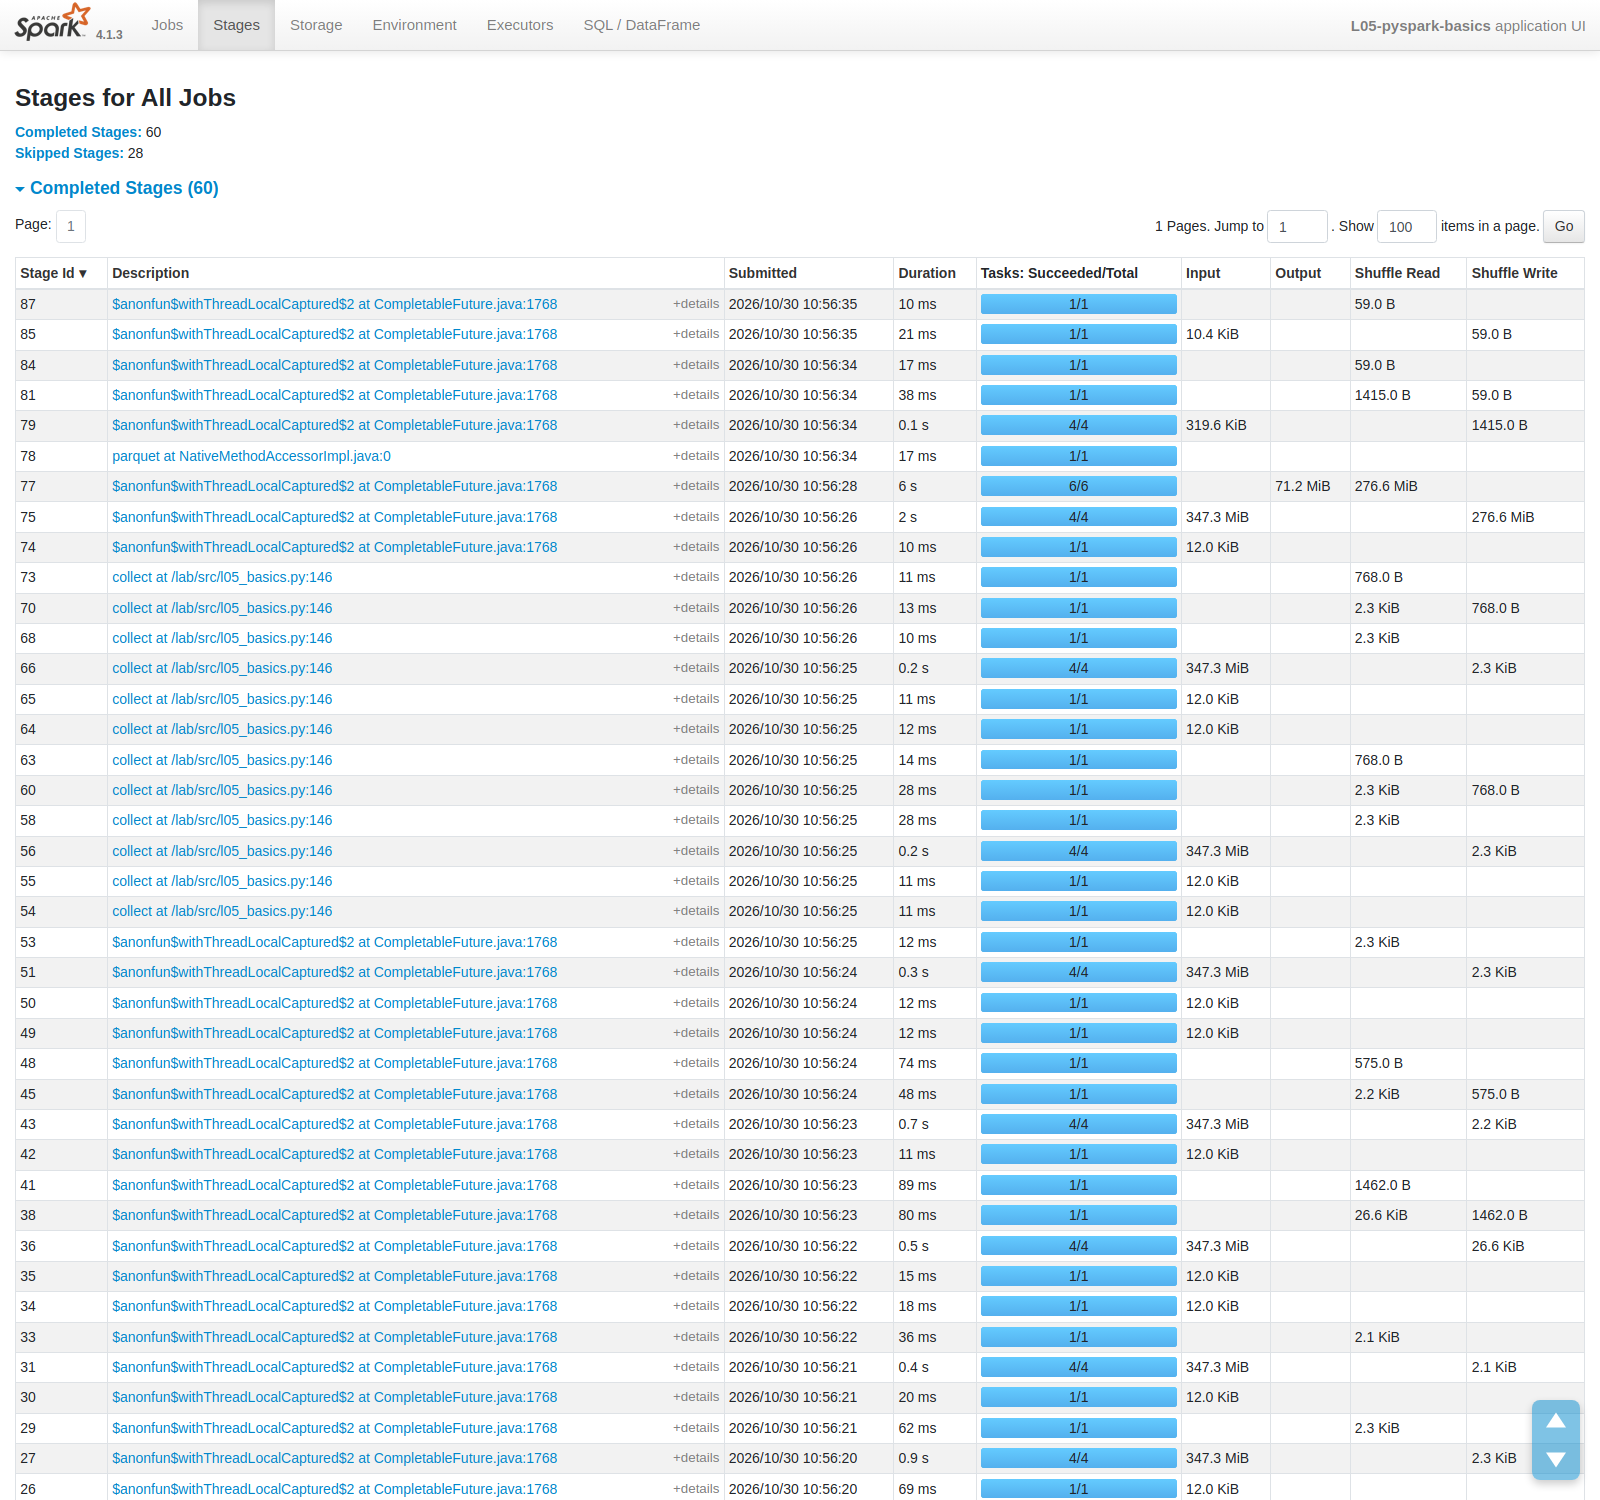
\includegraphics[keepaspectratio]{L05/img/21_ui_stages.png}}
& có cột Shuffle Read/Write; stage 4 task đọc từ cache \\
Storage &
\pandocbounded{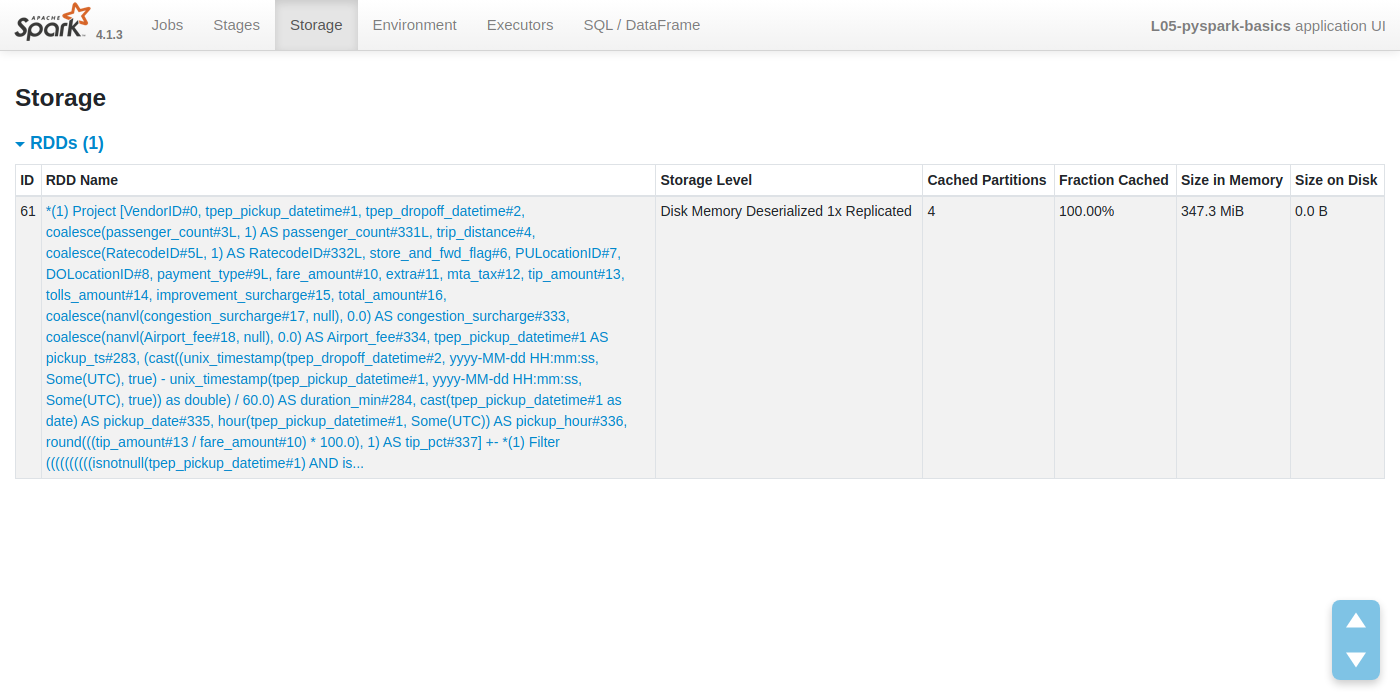
\includegraphics[keepaspectratio]{L05/img/22_ui_storage_cache.png}}
& DataFrame \texttt{clean} được cache: 4/4 partition, \textbf{100 \%},
\textbf{347.3 MiB} trong bộ nhớ \\
SQL (query 10 = \texttt{by\_borough.show()}) &
\pandocbounded{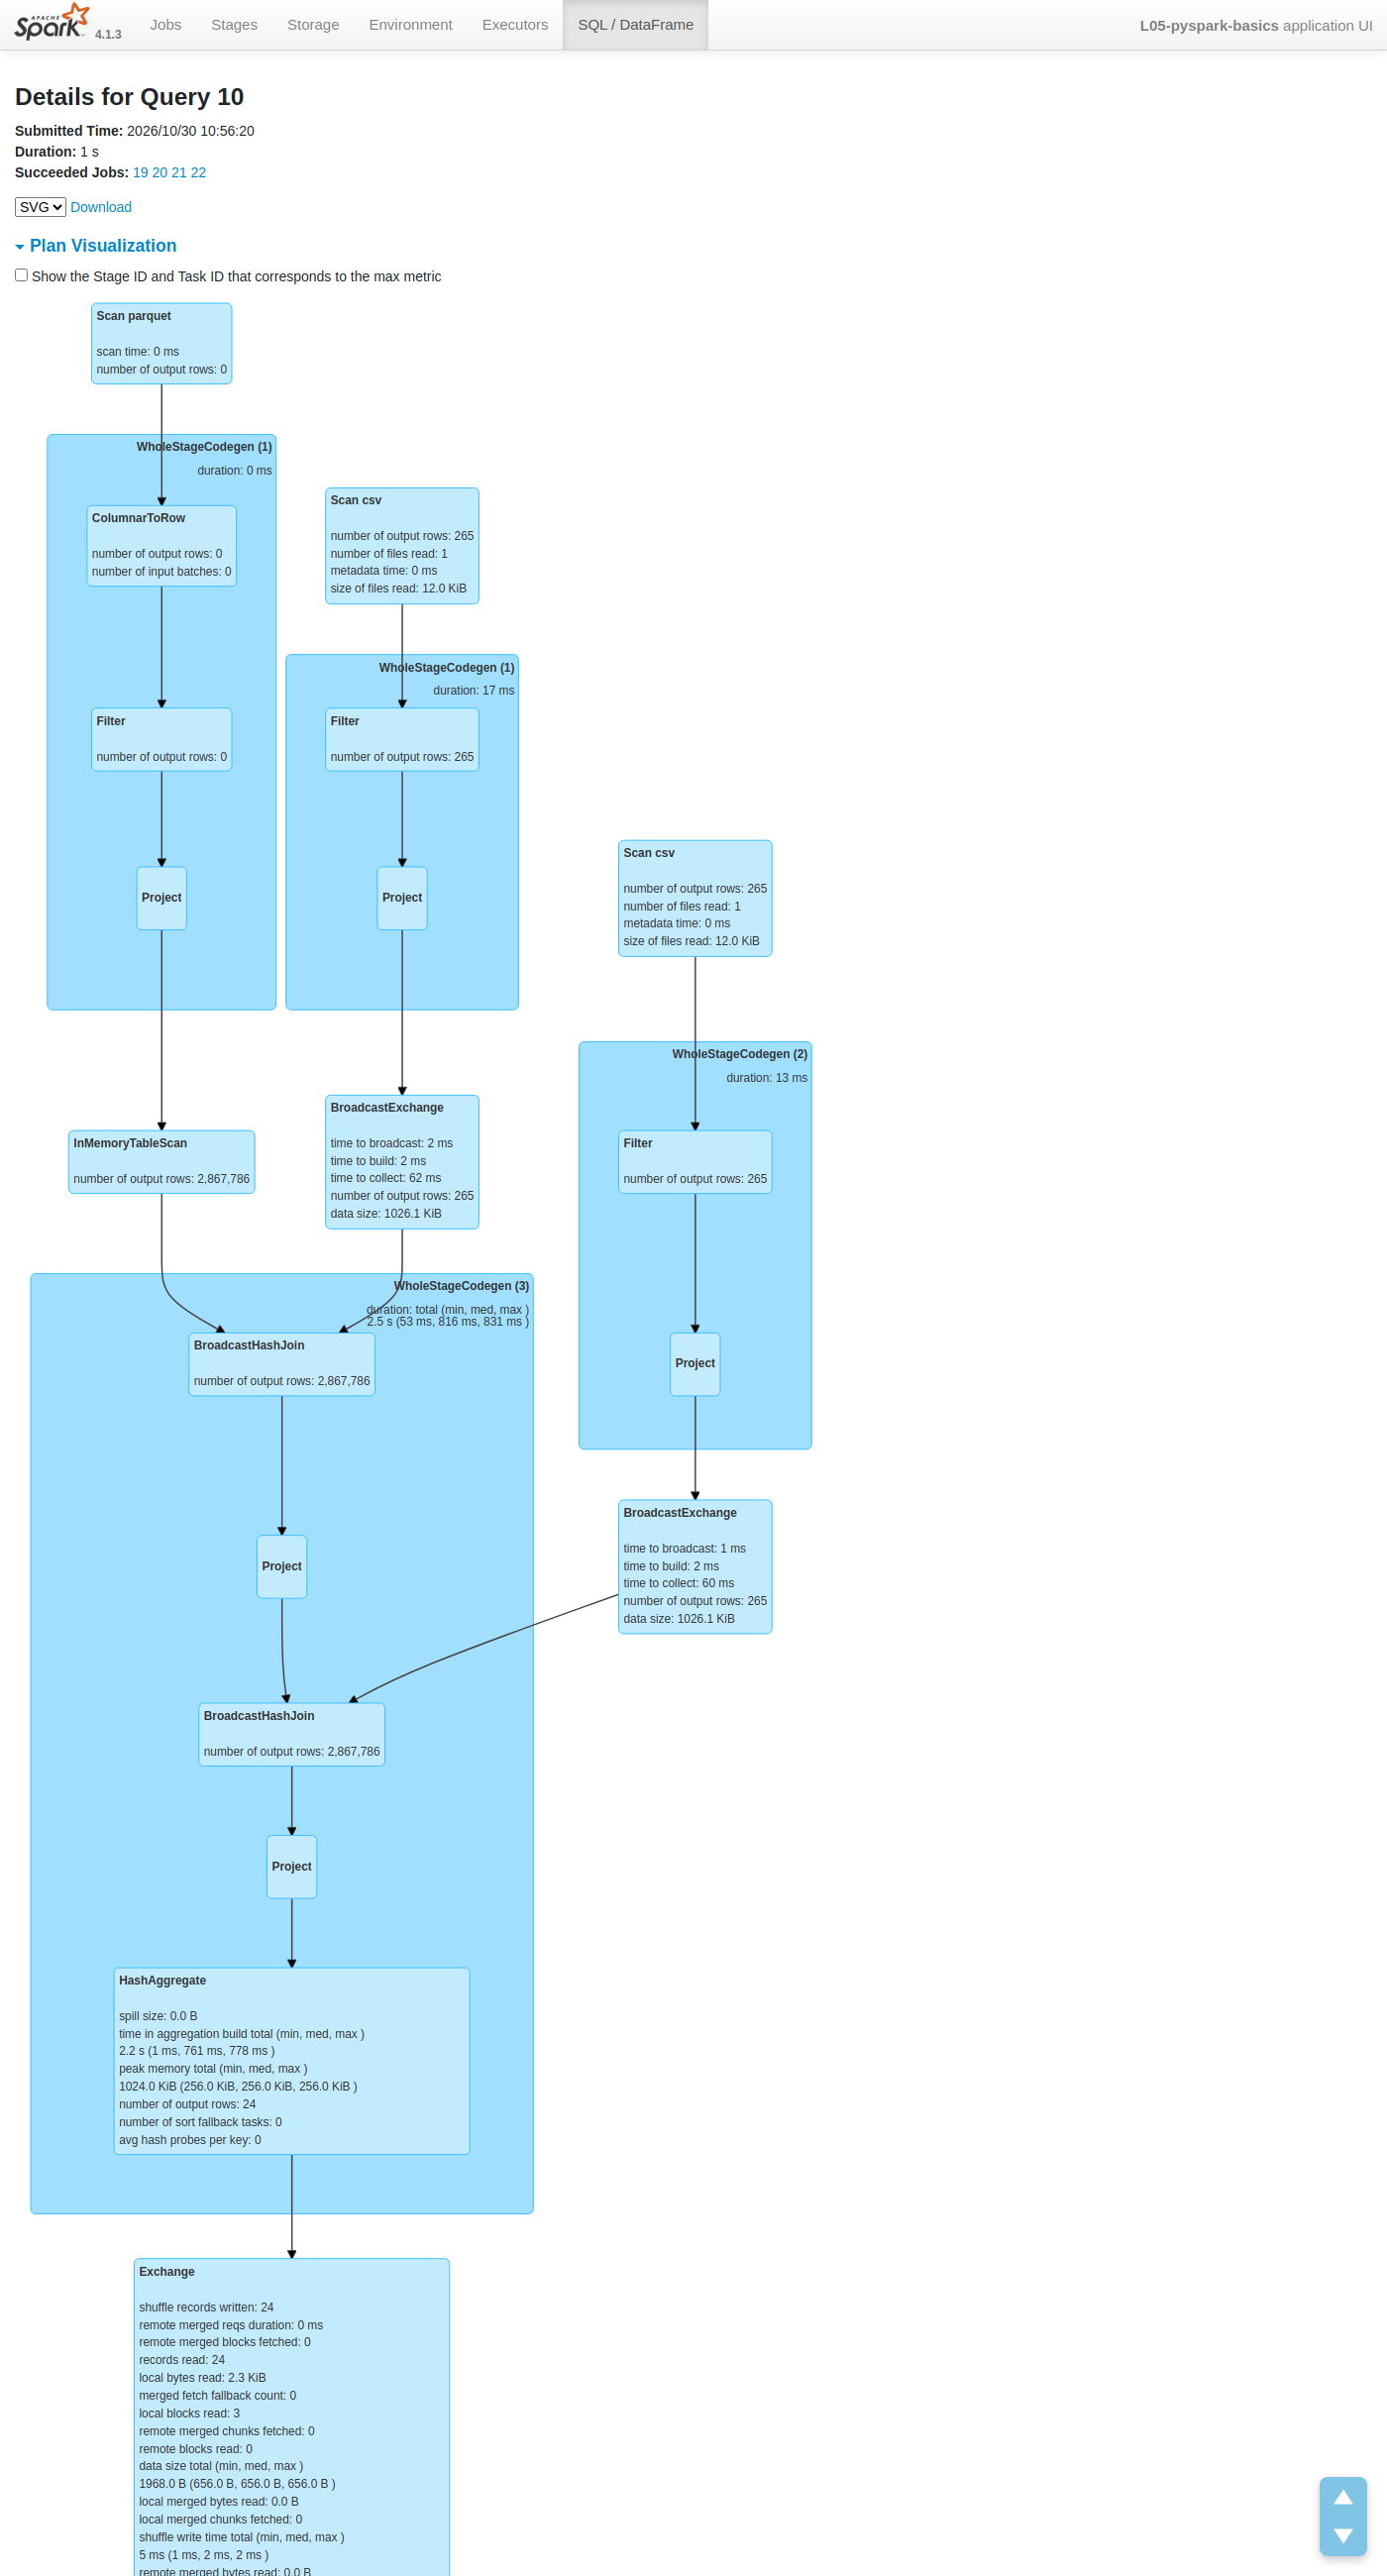
\includegraphics[keepaspectratio]{L05/img/24_ui_sql_by_borough_plan.png}}
& \texttt{InMemoryTableScan} 2,867,786 dòng → 2 ×
\texttt{BroadcastHashJoin} (265 dòng) → \texttt{HashAggregate} partial:
\textbf{24 dòng} → \texttt{Exchange} \\
Job 22 &
\pandocbounded{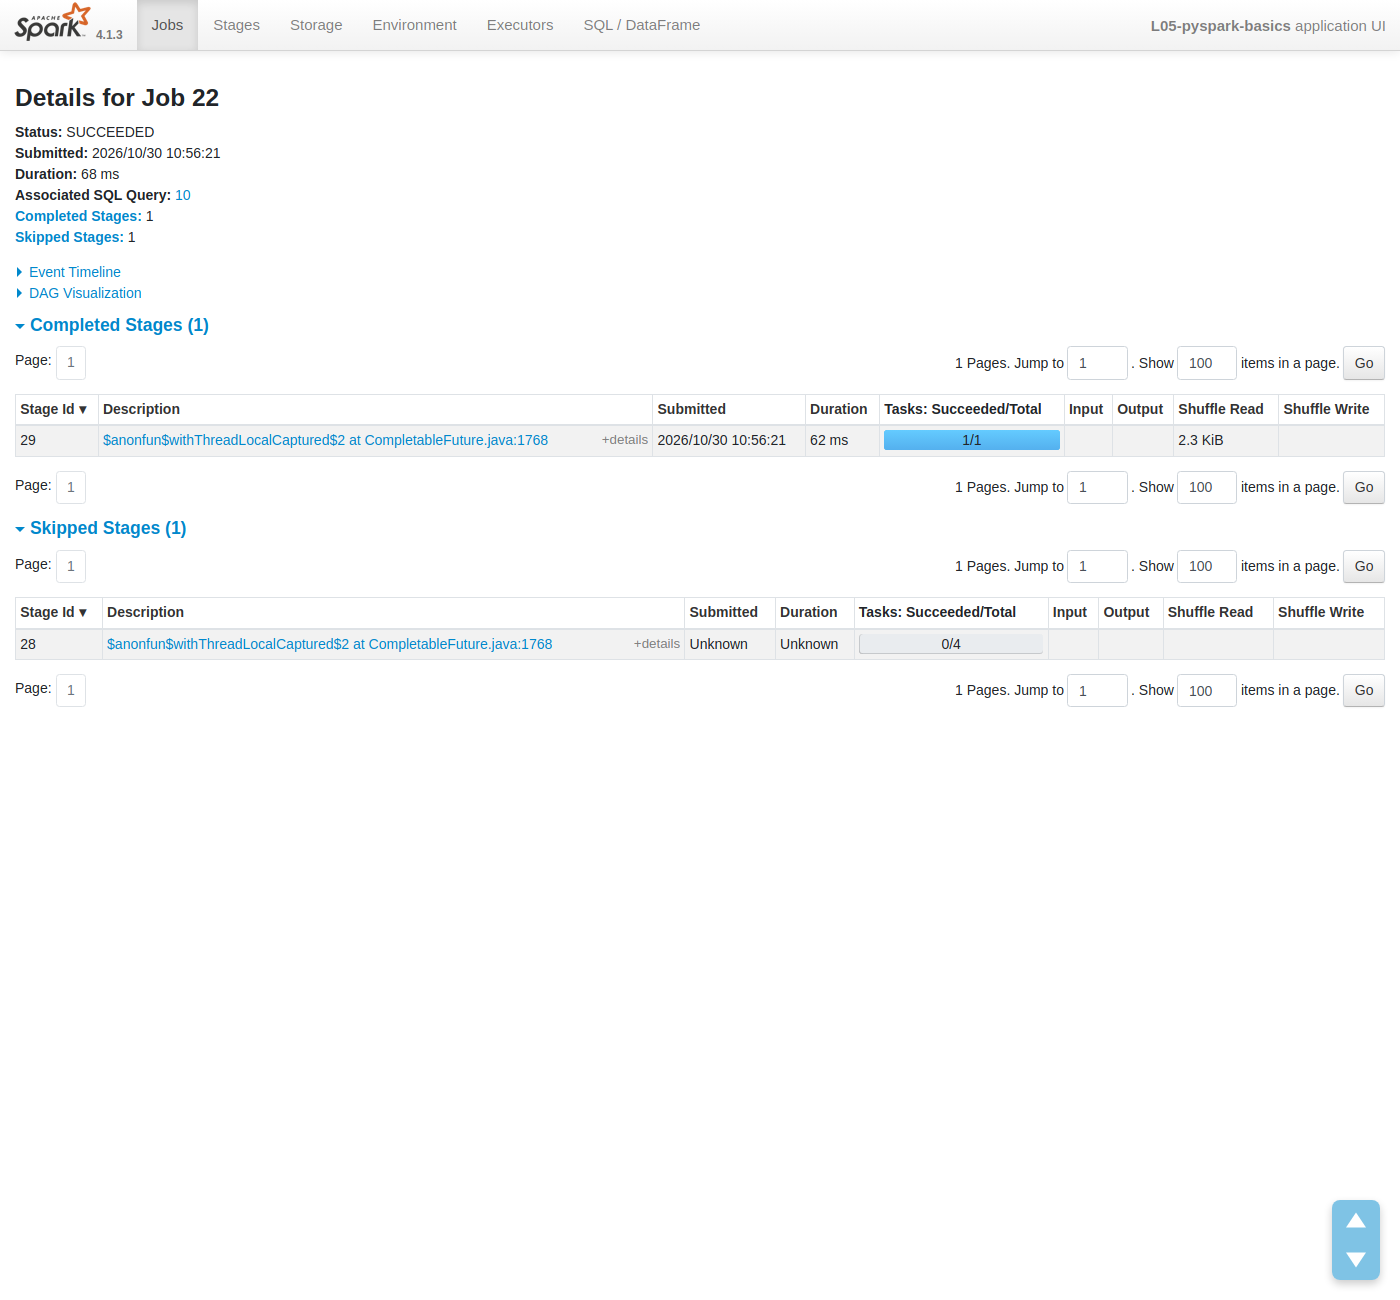
\includegraphics[keepaspectratio]{L05/img/28_ui_job22_dag.png}}
& stage 28 \emph{skipped} (dùng lại shuffle của job 21); stage 29 chạy 1
task, Shuffle Read 2.3 KiB \\
Khác &
\pandocbounded{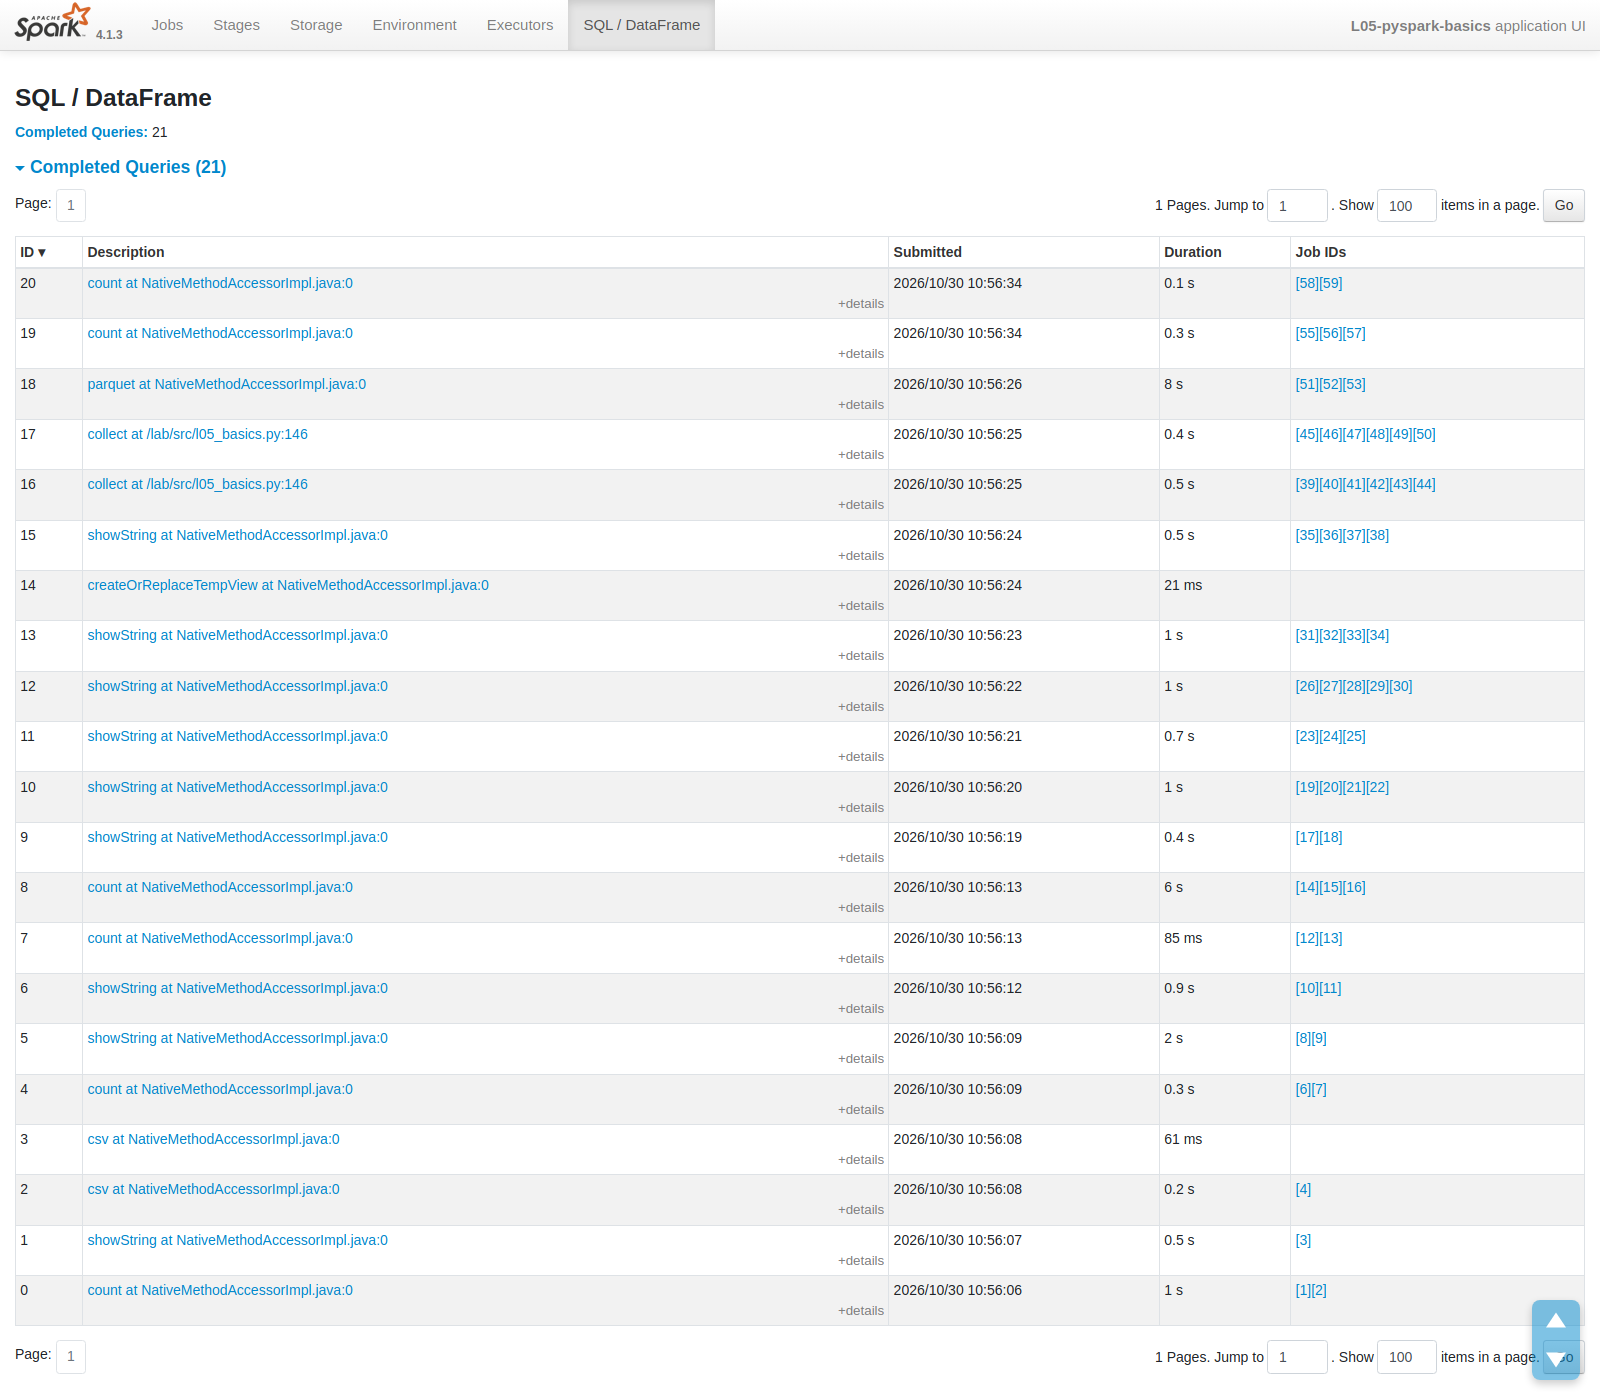
\includegraphics[keepaspectratio]{L05/img/23_ui_sql_list.png}}
\pandocbounded{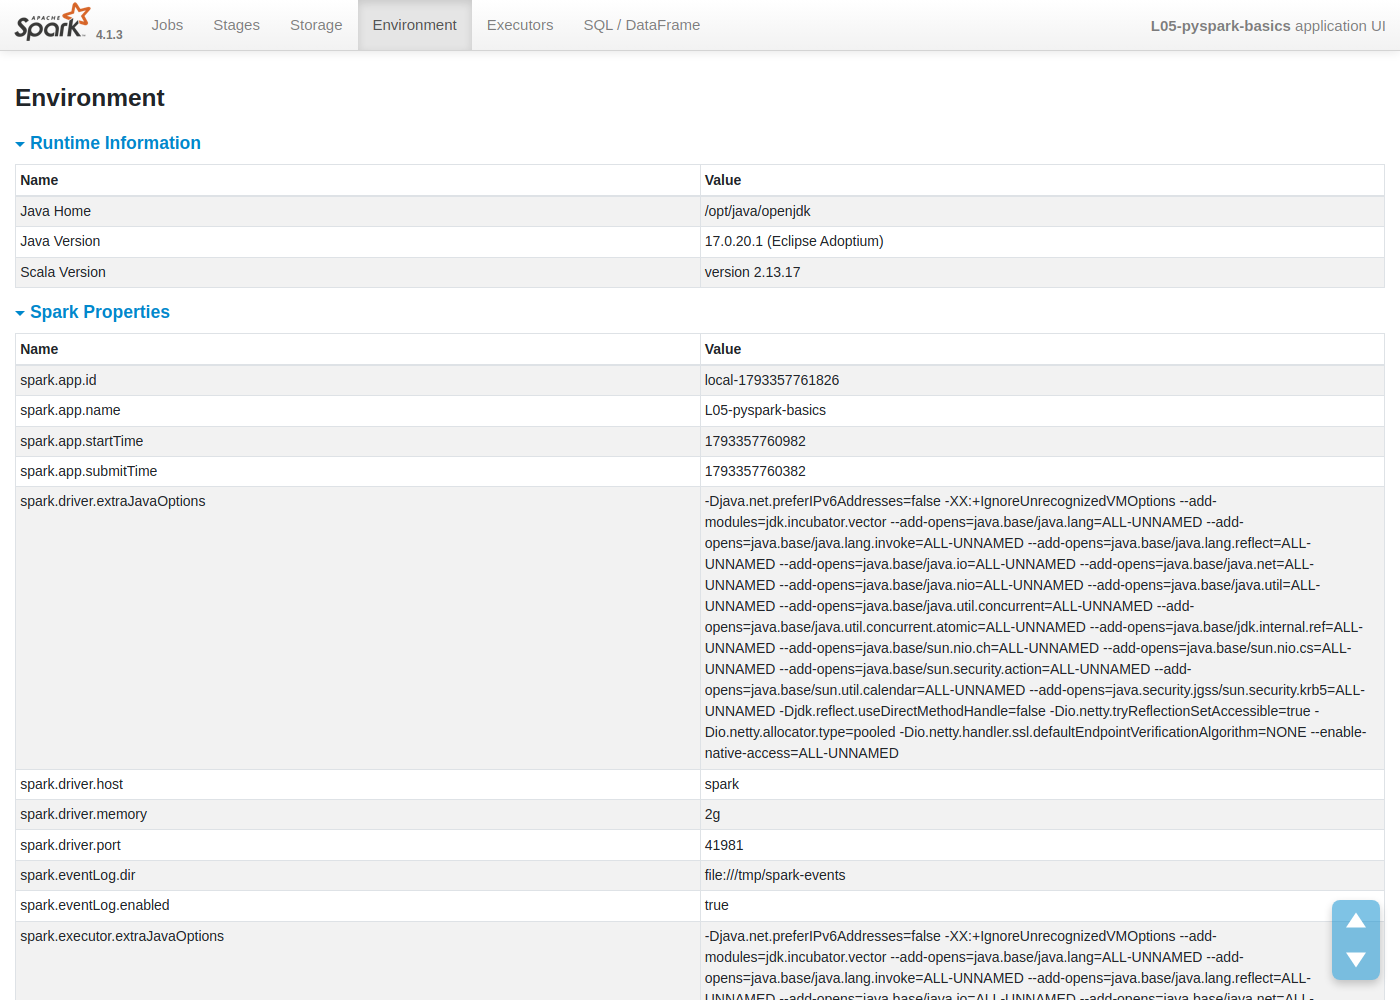
\includegraphics[keepaspectratio]{L05/img/25_ui_environment.png}}
\pandocbounded{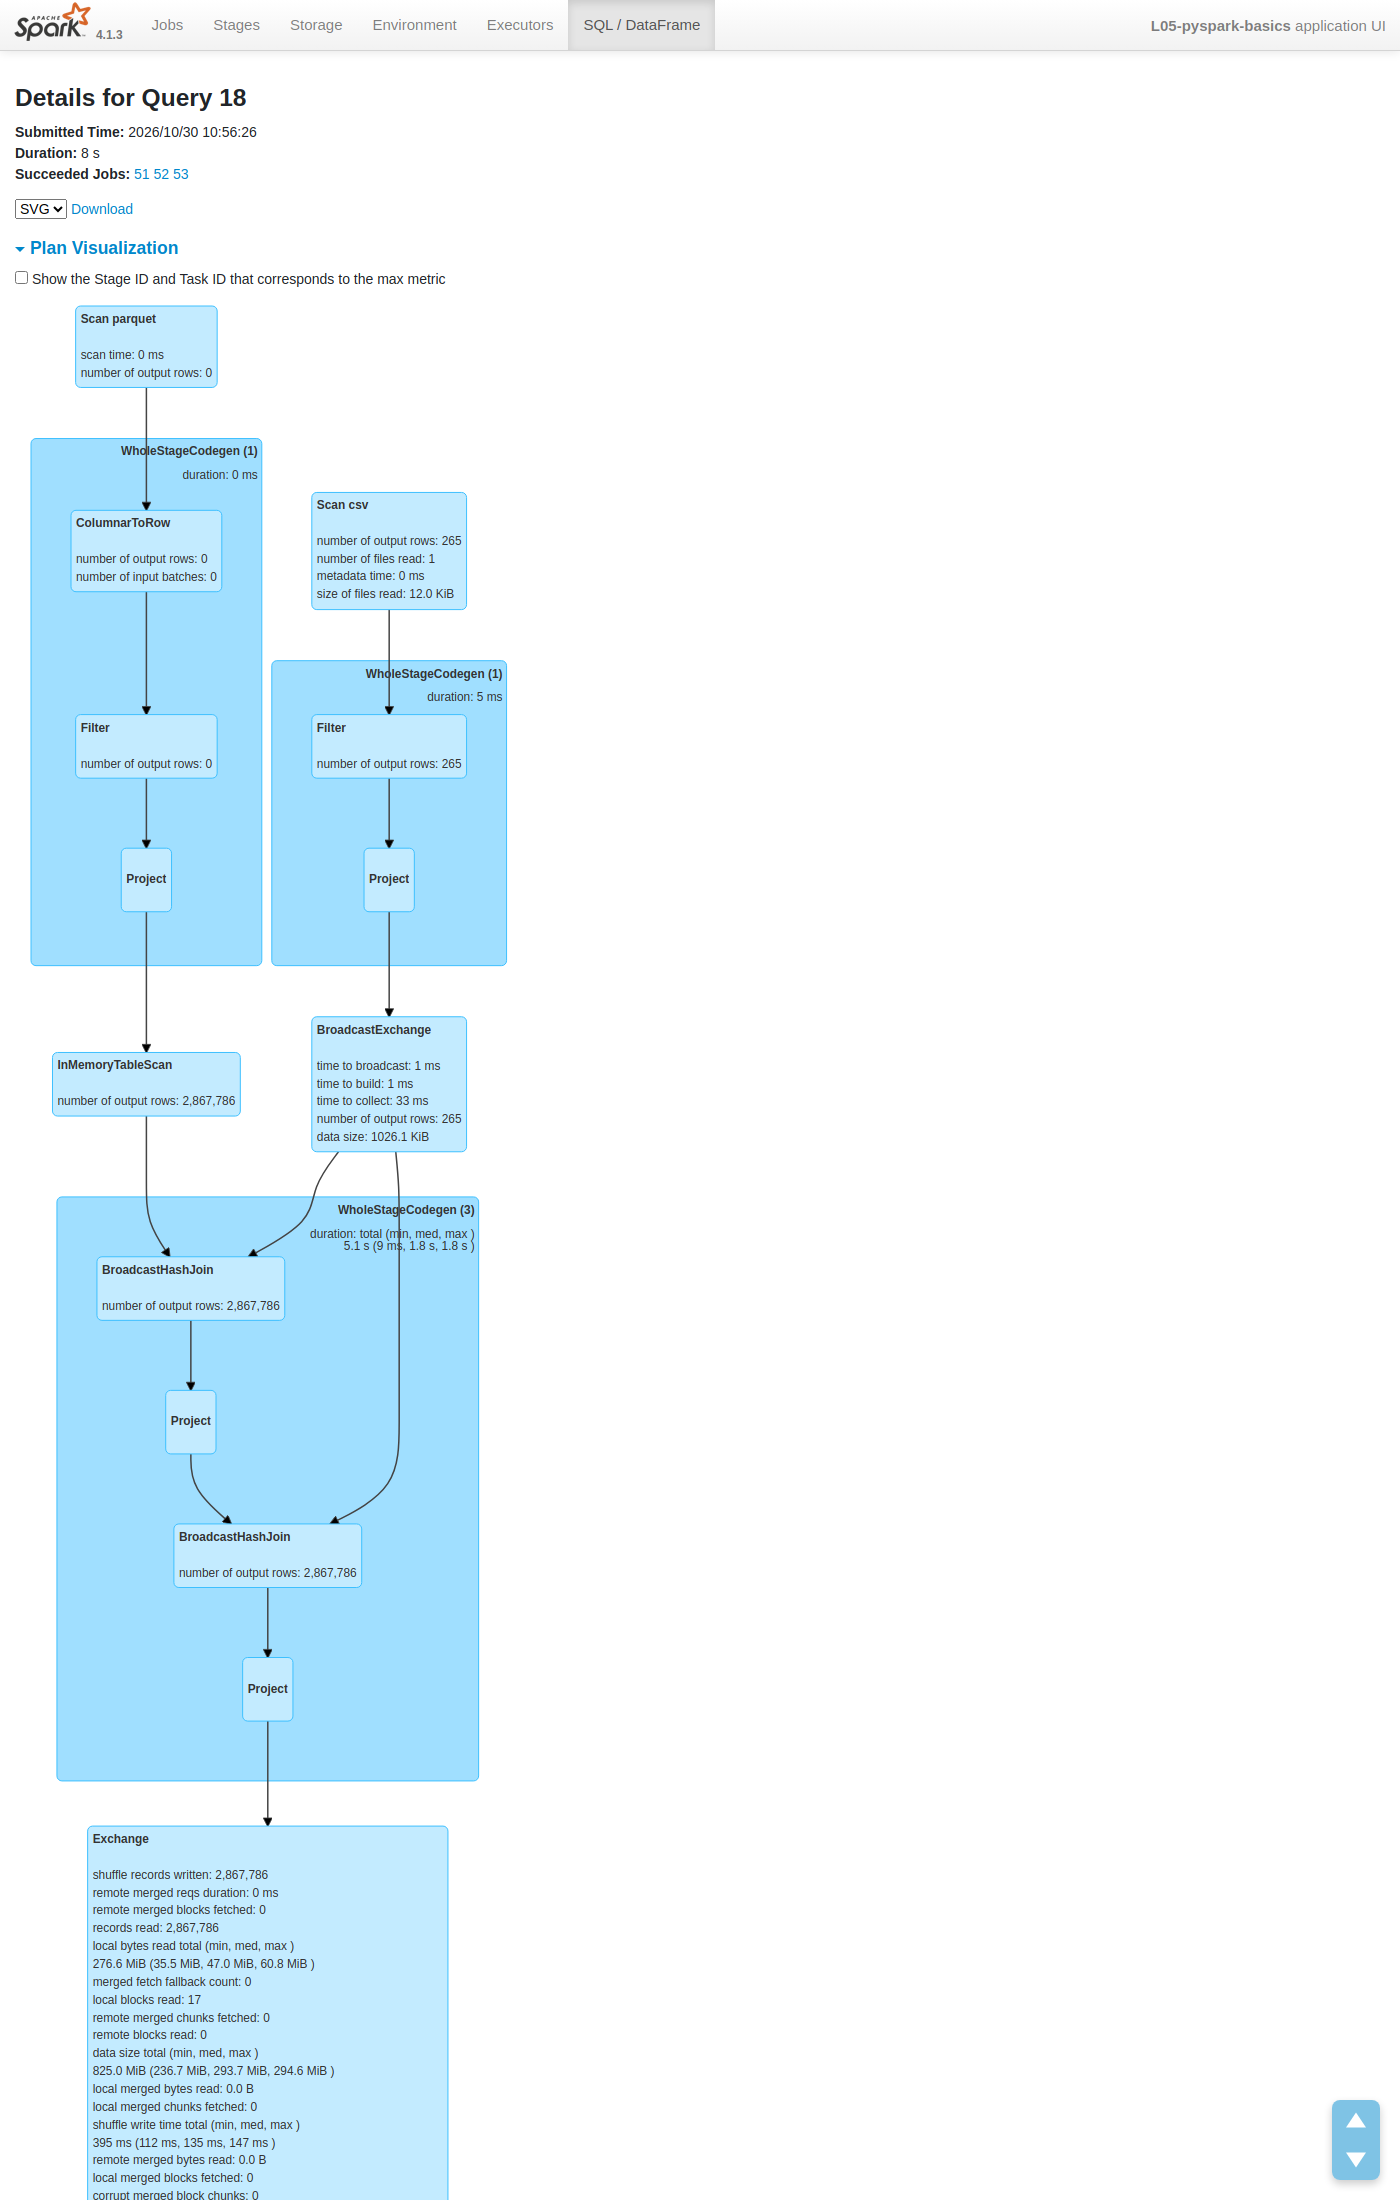
\includegraphics[keepaspectratio]{L05/img/26_ui_sql_write_parquet.png}}
\pandocbounded{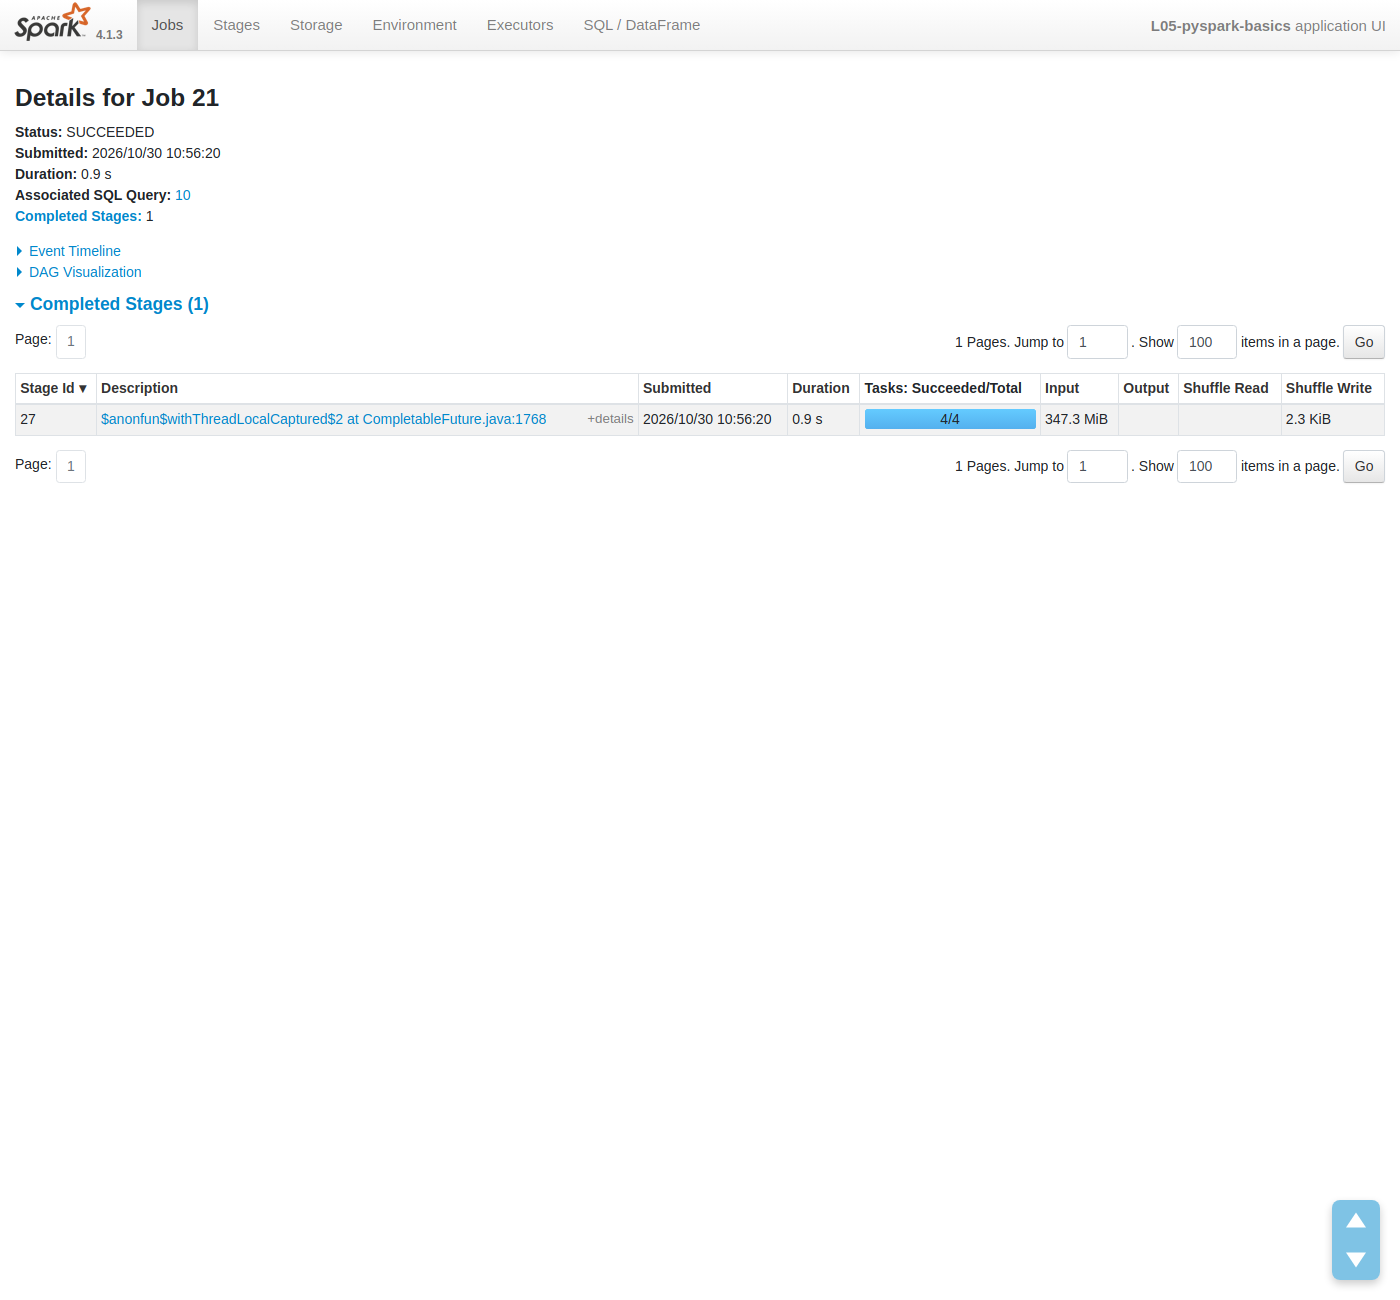
\includegraphics[keepaspectratio]{L05/img/27_ui_job21_dag.png}}
& \\
\end{longtable}

\subsection{Ghi Parquet phân vùng (TODO
7)}\label{ghi-parquet-phuxe2n-vuxf9ng-todo-7}

\begin{longtable}[]{@{}lll@{}}
\toprule\noalign{}
& Không \texttt{repartition} & \texttt{repartition("pickup\_date")} \\
\midrule\noalign{}
\endhead
\bottomrule\noalign{}
\endlastfoot
Số file \texttt{.parquet} & \textbf{56} & \textbf{31} (1 file/ngày) \\
File trong \texttt{pickup\_date=2024-01-15} & 2 & 1 \\
Dung lượng & 74 MB & 73 MB \\
Thời gian ghi & 6.8 s & 8.2 s (thêm 1 shuffle) \\
\end{longtable}

\begin{figure}
\centering
\pandocbounded{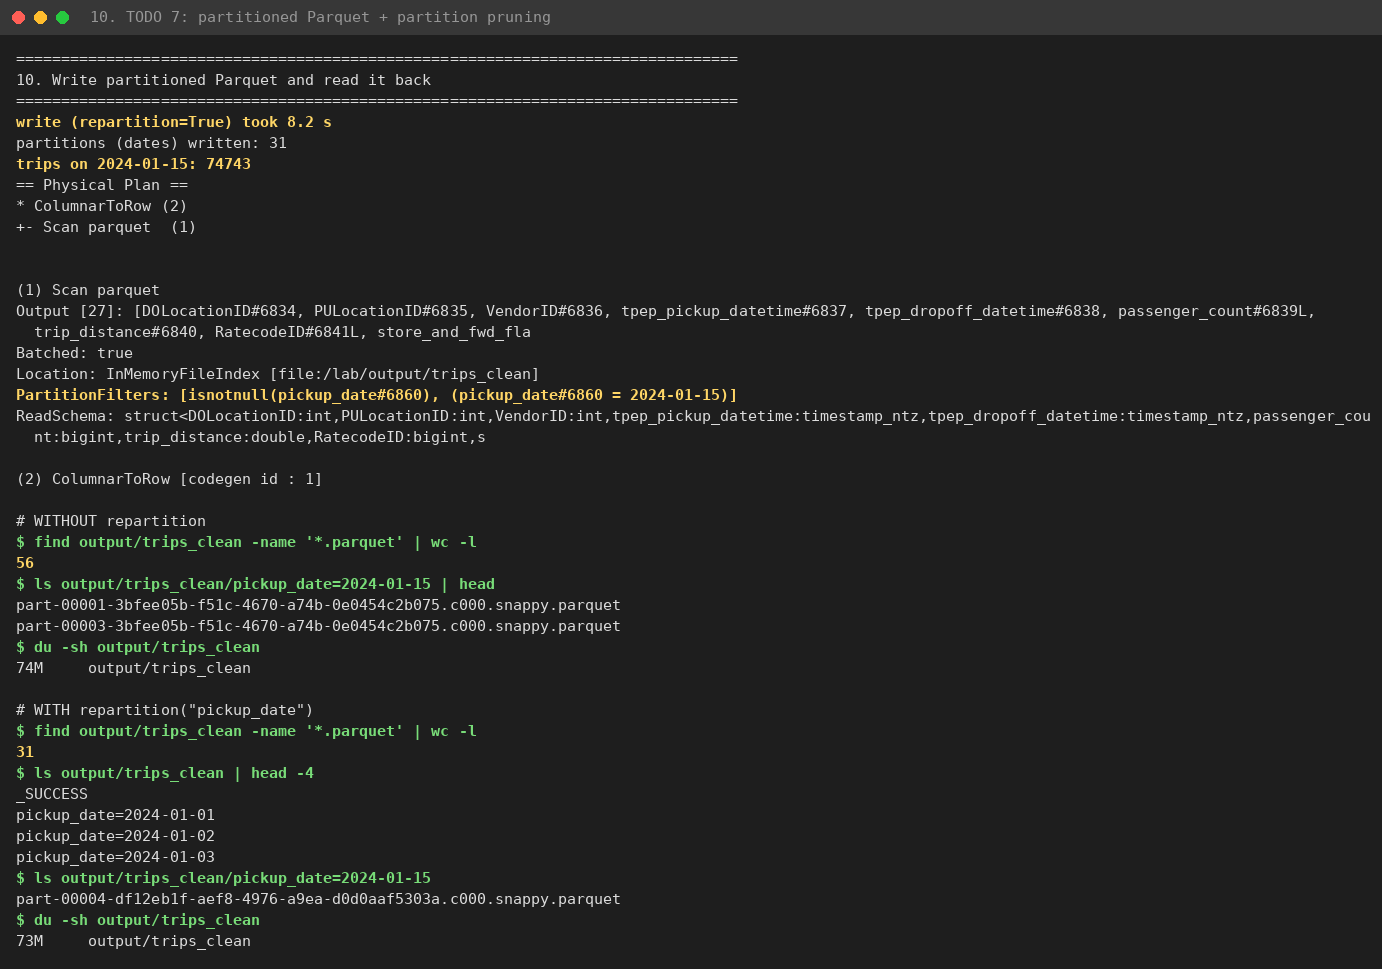
\includegraphics[keepaspectratio]{L05/img/07_write_partitioned_pruning.png}}
\caption{write + pruning}
\end{figure}

Không \texttt{repartition}, mỗi task trong 4 task ghi một file cho
\textbf{mỗi ngày mà nó chứa}. Ở đây chỉ ra 56 file chứ không phải 4 × 31
= 124, vì file nguồn gần như đã sắp theo thời gian: mỗi task chỉ chứa
một khoảng ngày liền nhau, và các ngày ở ranh giới bị tách thành 2 file.
Với dữ liệu không có thứ tự và hàng trăm task, số file sẽ là N × 31. Khi
đọc lại,
\texttt{PartitionFilters:\ {[}isnotnull(pickup\_date),\ (pickup\_date\ =\ 2024-01-15){]}}
cho thấy Spark chỉ mở \textbf{một thư mục}.

\subsection{Trả lời checkpoint}\label{trux1ea3-lux1eddi-checkpoint-4}

\textbf{Q1.} Spark chia file thành input partition dựa trên: -
\texttt{spark.sql.files.maxPartitionBytes}, mặc định 128 MB; - mục tiêu
có ít nhất \texttt{defaultParallelism} split (= 4 core với
\texttt{local{[}4{]}}), nên kích thước split được hạ xuống khoảng 48 MB
/ 4.

Parquet chỉ cắt được ở ranh giới \textbf{row group}: task nào nhận được
điểm bắt đầu của row group thì đọc row group đó. Vì vậy dù chỉ có một
file 48 MB vẫn ra \textbf{4 partition}, và một partition có thể rỗng nếu
số row group ít hơn 4.

\textbf{Q2.} \texttt{filter}, \texttt{withColumn} và \texttt{select} là
\textbf{transformation}: chúng chỉ thêm node vào logical plan, không
đụng tới dữ liệu, nên mất 0.096 s. \texttt{count()} là \textbf{action}:
Catalyst tối ưu plan, DAG scheduler tạo stage và task, rồi mới đọc file
(0.28 s). \texttt{show}, \texttt{collect}, \texttt{take}, \texttt{write}
và \texttt{count} cũng là action. Plan dựng trong vài mili-giây vì đó
chỉ là thao tác trên cây biểu thức trong bộ nhớ của driver.

\textbf{Q3 (lazy evaluation và DAG).} \texttt{by\_borough.show()} là SQL
query 10. Nó sinh ra \textbf{4 job} (19--22) với AQE:

\begin{longtable}[]{@{}
  >{\raggedright\arraybackslash}p{(\linewidth - 6\tabcolsep) * \real{0.2500}}
  >{\raggedright\arraybackslash}p{(\linewidth - 6\tabcolsep) * \real{0.2500}}
  >{\raggedright\arraybackslash}p{(\linewidth - 6\tabcolsep) * \real{0.2500}}
  >{\raggedright\arraybackslash}p{(\linewidth - 6\tabcolsep) * \real{0.2500}}@{}}
\toprule\noalign{}
\begin{minipage}[b]{\linewidth}\raggedright
Job
\end{minipage} & \begin{minipage}[b]{\linewidth}\raggedright
Stage
\end{minipage} & \begin{minipage}[b]{\linewidth}\raggedright
Số task
\end{minipage} & \begin{minipage}[b]{\linewidth}\raggedright
Việc làm
\end{minipage} \\
\midrule\noalign{}
\endhead
\bottomrule\noalign{}
\endlastfoot
19 & 25 & 1 & dựng broadcast bảng zone cho \textbf{pickup}
(\texttt{BroadcastExchange}) \\
20 & 26 & 1 & dựng broadcast bảng zone cho \textbf{dropoff} \\
21 & 27 & \textbf{4} & đọc \texttt{InMemoryTableScan} (cache), 2 ×
\texttt{BroadcastHashJoin}, \texttt{HashAggregate} partial, \textbf{ghi
shuffle} (\texttt{Exchange\ hashpartitioning(pu\_borough,\ 8)}) \\
22 & 28 (skipped, dùng lại output của 27), \textbf{29} & 1 &
\texttt{AQEShuffleRead\ coalesced} (8 → 1 partition),
\texttt{HashAggregate} final, \texttt{TakeOrderedAndProject} cho
\texttt{orderBy\ +\ show} \\
\end{longtable}

\begin{itemize}
\tightlist
\item
  \textbf{Ranh giới stage là các toán tử \texttt{Exchange} (shuffle).}
\item
  Broadcast chạy thành job riêng.
\item
  Với AQE, mỗi query stage được nộp thành một job riêng, nên stage của
  job trước hiện là \emph{skipped} trong job sau.
\item
  Khi chạy toàn bộ \texttt{by\_borough} (ví dụ \texttt{collect}), plan
  còn có \texttt{Exchange\ rangepartitioning(trips\ DESC,\ 8)} cho
  \texttt{orderBy}, tức là thêm một stage sort nữa (xem
  \texttt{explain}).
\item
  Không có gì chạy cho tới khi gọi \texttt{show()}. Các transformation ở
  mục 4--5 chỉ dựng DAG.
\end{itemize}

\textbf{Q4.} 5 cột có cùng 140,162 NULL vì đó là \textbf{cùng 140,162
chuyến}. Các bản ghi này được gửi lên thiếu toàn bộ nhóm trường
``metadata'' (thường từ một vendor hoặc từ chuyến street-hail), chứ
không phải 5 lỗi độc lập. Có ba cách xử lý: - giữ lại và gán mặc định,
như script làm: \texttt{passenger\_count=1}, \texttt{RatecodeID=1}, phụ
phí = 0; - giữ NULL và chỉ loại khỏi các chỉ số cần những cột đó; - tách
ra vùng quarantine.

Cách nào cũng cần thống nhất với chủ dữ liệu và ghi lại trong tài liệu.

\textbf{Q5 (đọc formatted plan).} Đọc từ dưới lên: 1.
\texttt{Scan\ parquet} với \texttt{PushedFilters}
(\texttt{GreaterThan(fare\_amount,0.0)},
\texttt{LessThanOrEqual(trip\_distance,100.0)}\ldots): luật làm sạch
được đẩy xuống reader Parquet. 2. \texttt{InMemoryTableScan}: đọc từ
cache. 3. 2 × \texttt{BroadcastExchange} và
\texttt{BroadcastHashJoin\ LeftOuter\ BuildRight}. 4.
\texttt{HashAggregate} (22) với
\texttt{partial\_count(1),\ partial\_avg(...)}. Mỗi task \textbf{gộp
trước} các dòng của nó theo \texttt{pu\_borough}. \texttt{avg} được tách
thành cặp \texttt{(sum,\ count)}, nên mỗi task chỉ phát ra khoảng 6--8
dòng; tổng cộng \textbf{24 dòng} đi qua shuffle thay vì 2.87 triệu. 5.
\texttt{Exchange\ hashpartitioning(pu\_borough,\ 8)}: \textbf{shuffle},
cũng là ranh giới stage. 6. \texttt{AQEShuffleRead\ coalesced}: AQE gộp
8 partition shuffle nhỏ lại. 7. \texttt{HashAggregate} (26) final với
\texttt{count(1),\ avg(...)}: gộp các kết quả partial. 8.
\texttt{Exchange\ rangepartitioning} và \texttt{Sort} cho
\texttt{orderBy}.

Partial/final aggregate chính là \textbf{combiner của L02}. Tách
\texttt{avg} thành \texttt{(sum,\ count)} cũng giống hệt cách làm ở bài
stretch L02 (combiner tính giá cước trung bình).

\textbf{Q6.} Bảng zone chỉ có 265 dòng (12 KB, khoảng 1 MB trong bộ nhớ
theo \texttt{Statistics(sizeInBytes=1026.1\ KiB)}), nhỏ hơn nhiều so với
\texttt{spark.sql.autoBroadcastJoinThreshold} (10 MB). Spark gửi một bản
sao cho mọi task, nên 2.87 triệu chuyến \textbf{không phải shuffle}. Khi
cả hai bên đều lớn hơn ngưỡng (hoặc đặt ngưỡng = -1, hoặc thống kê kích
thước vượt ngưỡng), Spark shuffle cả hai bên theo key và dùng
\textbf{SortMergeJoin}. L06 đo sự khác biệt này.

\textbf{Q7.} Sau khi \texttt{cache()}: - \textbf{Plan} đọc từ
\texttt{InMemoryRelation}/\texttt{InMemoryTableScan} thay vì quét và lọc
lại Parquet. - \textbf{Tab Storage} hiện RDD đã cache: 4 partition, 100
\%, 347.3 MiB. - Các action sau nhanh hơn, ví dụ \texttt{clean.count()}
lần đầu (materialize cache) mất khoảng 6 s, còn các query sau chỉ
0.3--1.5 s.

Cache là ý tồi khi: - dữ liệu chỉ dùng một lần; - dữ liệu không vừa bộ
nhớ, gây spill, eviction và áp lực GC (347 MiB cache so với 48 MB
Parquet nén là hệ số khoảng 7×); - đọc nguồn vốn đã rẻ (Parquet có
column pruning có thể nhanh hơn cache dạng hàng rộng); - quên
\texttt{unpersist()}, làm giữ bộ nhớ không cần thiết.

\textbf{Q8.} \texttt{partitionBy} ghi \textbf{một file cho mỗi task ×
mỗi giá trị partition} mà task đó chứa. Không \texttt{repartition}, mỗi
task có thể chứa dòng của nhiều ngày, và số file có thể lên tới N task ×
31 ngày. Ở đây đo được 56 file; trên cluster thật sẽ là hàng nghìn file
nhỏ, gây hại cho NameNode và cho tốc độ đọc.
\texttt{repartition("pickup\_date")} shuffle trước để mọi dòng của một
ngày về cùng một task, nên ra \textbf{đúng 1 file/ngày (31 file)}. Cái
giá là thêm một shuffle (6.8 s → 8.2 s). Cần cẩn thận khi một giá trị
quá lớn (skew): một task sẽ phải ghi cả file khổng lồ. Khi đó dùng
\texttt{repartition(n,\ "pickup\_date",\ salt)} hoặc
\texttt{maxRecordsPerFile}.

\newpage

\section{L06 --- Spark performance: shuffle, join, skew, AQE,
partitioning,
cache}\label{l06-spark-performance-shuffle-join-skew-aqe-partitioning-cache}

Môi trường: Spark 4.1.3 \texttt{local{[}4{]}}, driver 2 GB. Dữ liệu:
taxi 2024-01 (2.96 triệu dòng) và một fact tổng hợp 10 triệu dòng, trong
đó 60 \% có key = 0. Script được chạy \textbf{2 lần}; báo cáo dùng lần
2.

\subsection{File nộp}\label{file-nux1ed9p-3}

\begin{longtable}[]{@{}
  >{\raggedright\arraybackslash}p{(\linewidth - 2\tabcolsep) * \real{0.5000}}
  >{\raggedright\arraybackslash}p{(\linewidth - 2\tabcolsep) * \real{0.5000}}@{}}
\toprule\noalign{}
\begin{minipage}[b]{\linewidth}\raggedright
File
\end{minipage} & \begin{minipage}[b]{\linewidth}\raggedright
Nội dung
\end{minipage} \\
\midrule\noalign{}
\endhead
\bottomrule\noalign{}
\endlastfoot
\texttt{l06\_experiments.py} & TODO 1--4: E1 AQE on, E2 hint
\texttt{broadcast()}, E3 salting và AQE skew join \\
\texttt{results.csv} & 34 dòng (2 lần chạy × 17 variant) \\
\texttt{RESULTS.md} & bảng lần 2, nhận xét E1--E5, khuyến nghị cho
cluster 20 node \\
\texttt{01\_run1.txt}, \texttt{02\_run2.txt} & log console \\
\texttt{03\_e3\_task\_quantiles.txt} & phân vị thời gian task và số bản
ghi shuffle/task (REST API) \\
\end{longtable}

\begin{figure}
\centering
\pandocbounded{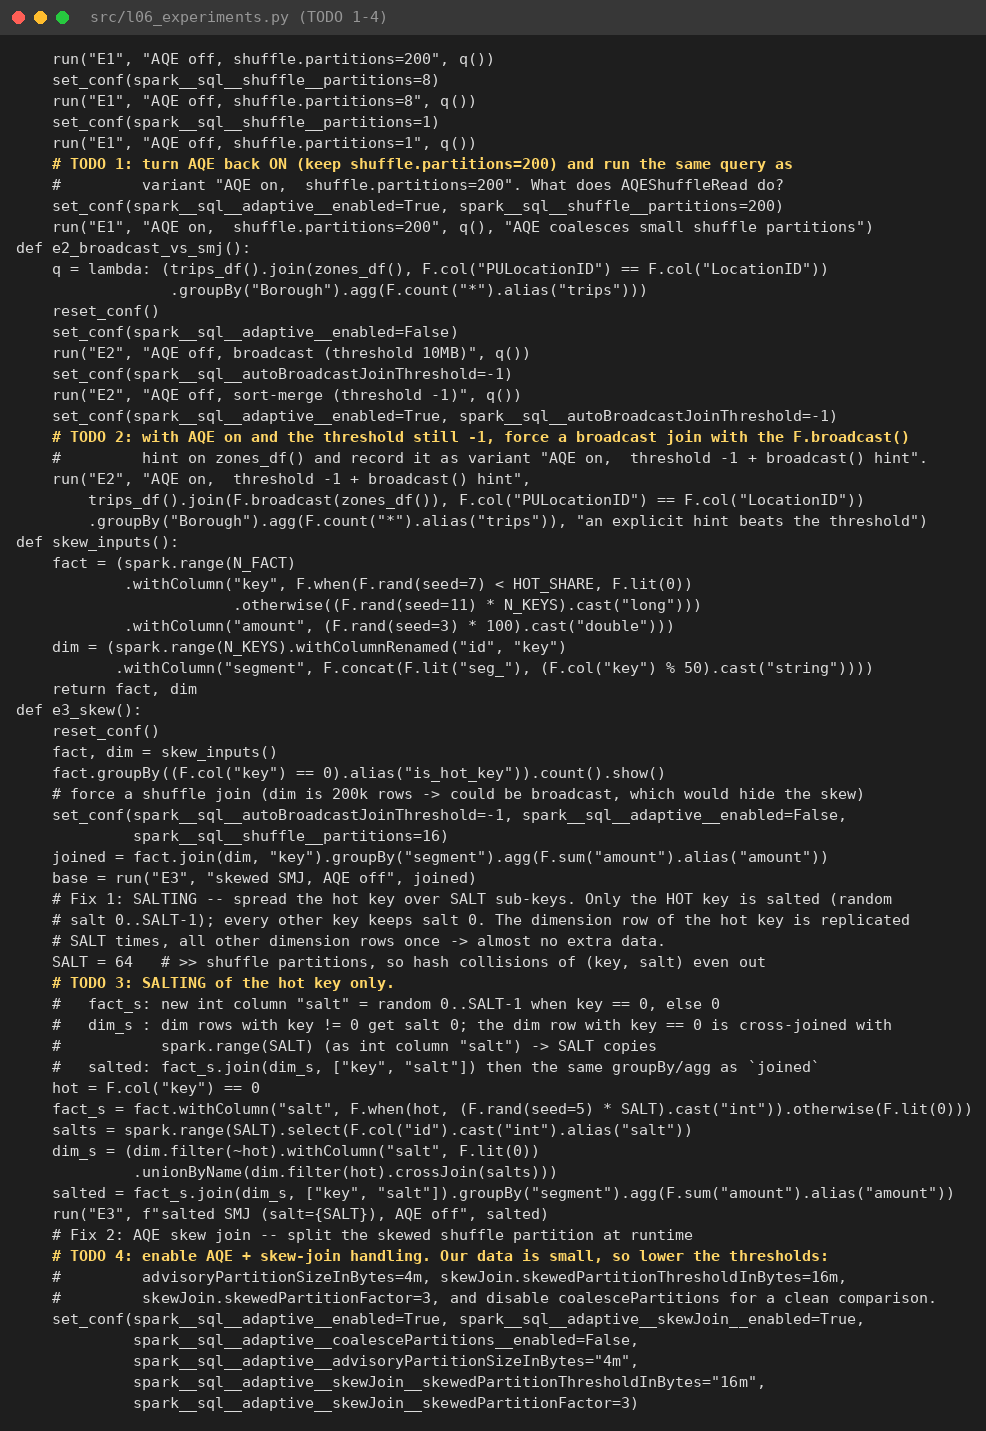
\includegraphics[keepaspectratio]{L06/img/code_l06_experiments.png}}
\caption{code}
\end{figure}

\subsection{Bảng kết quả (lần
2)}\label{bux1ea3ng-kux1ebft-quux1ea3-lux1ea7n-2}

\pandocbounded{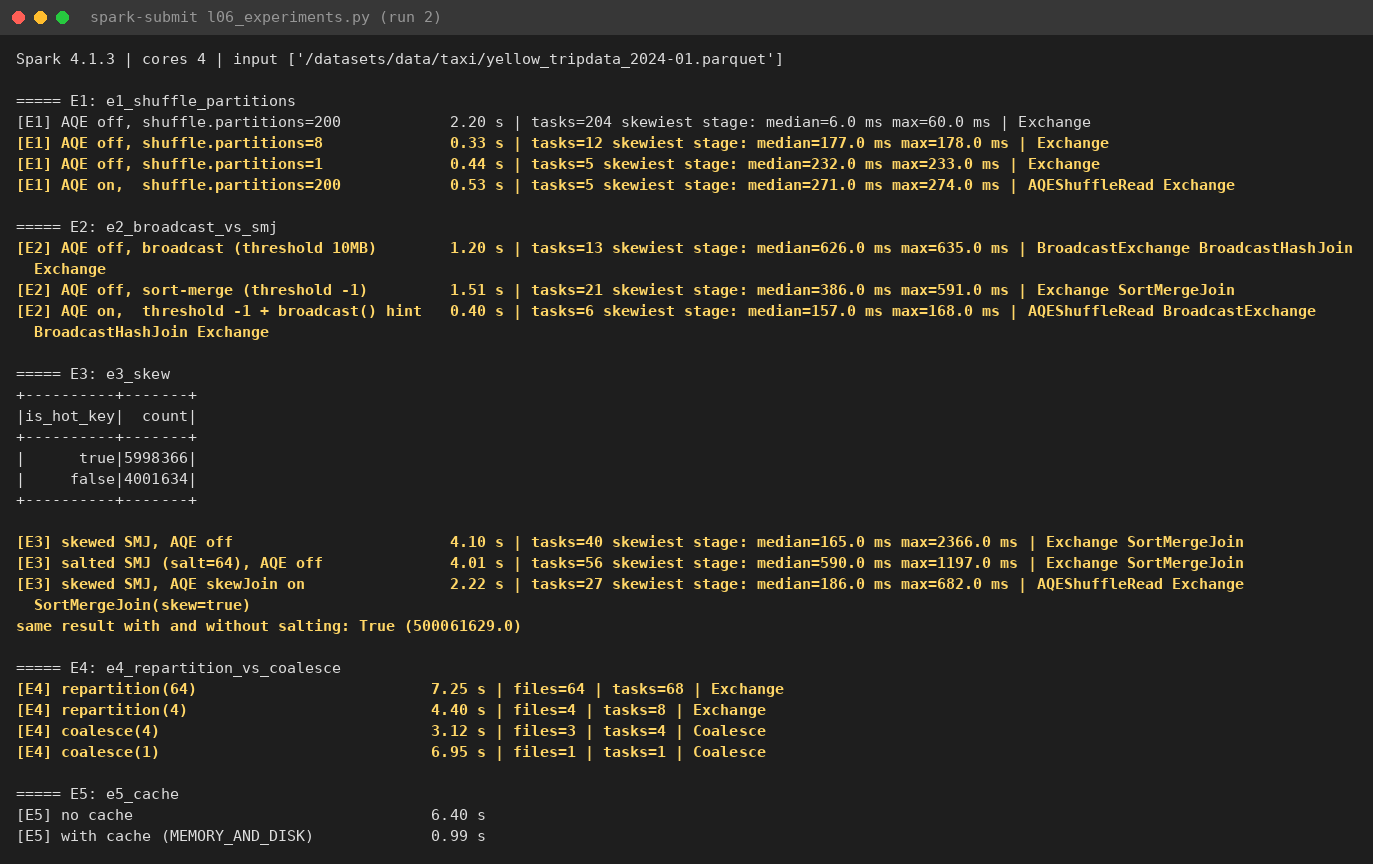
\includegraphics[keepaspectratio]{L06/img/01_run2_console.png}}
\pandocbounded{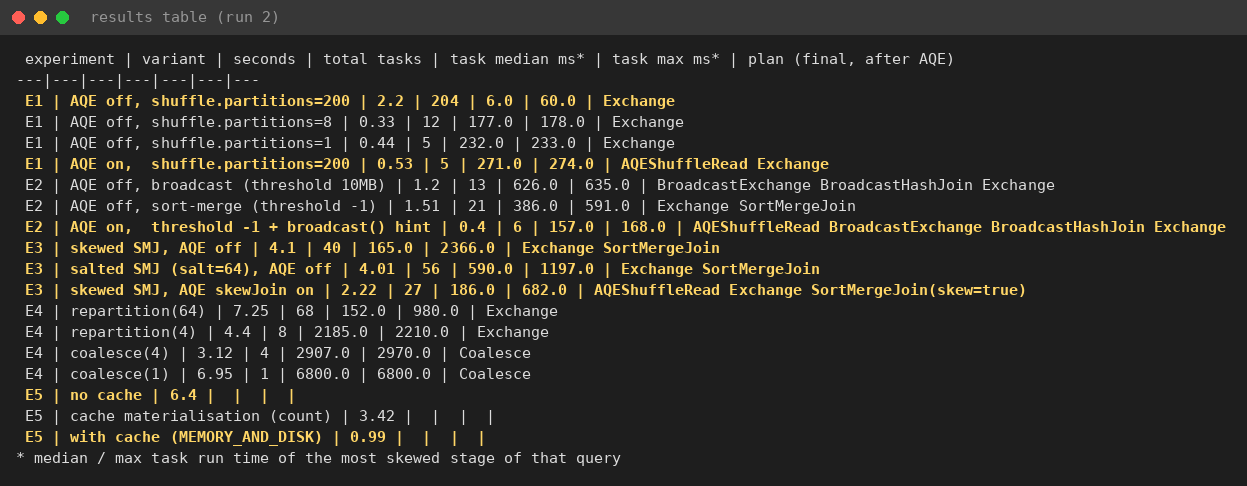
\includegraphics[keepaspectratio]{L06/img/02_run2_results_table.png}}

Bảng đầy đủ, nhận xét từng thí nghiệm và khuyến nghị nằm trong
\href{L06/RESULTS.md}{\texttt{RESULTS.md}}.

\subsection{Bằng chứng trên Spark
UI}\label{bux1eb1ng-chux1ee9ng-truxean-spark-ui}

\begin{figure}
\centering
\pandocbounded{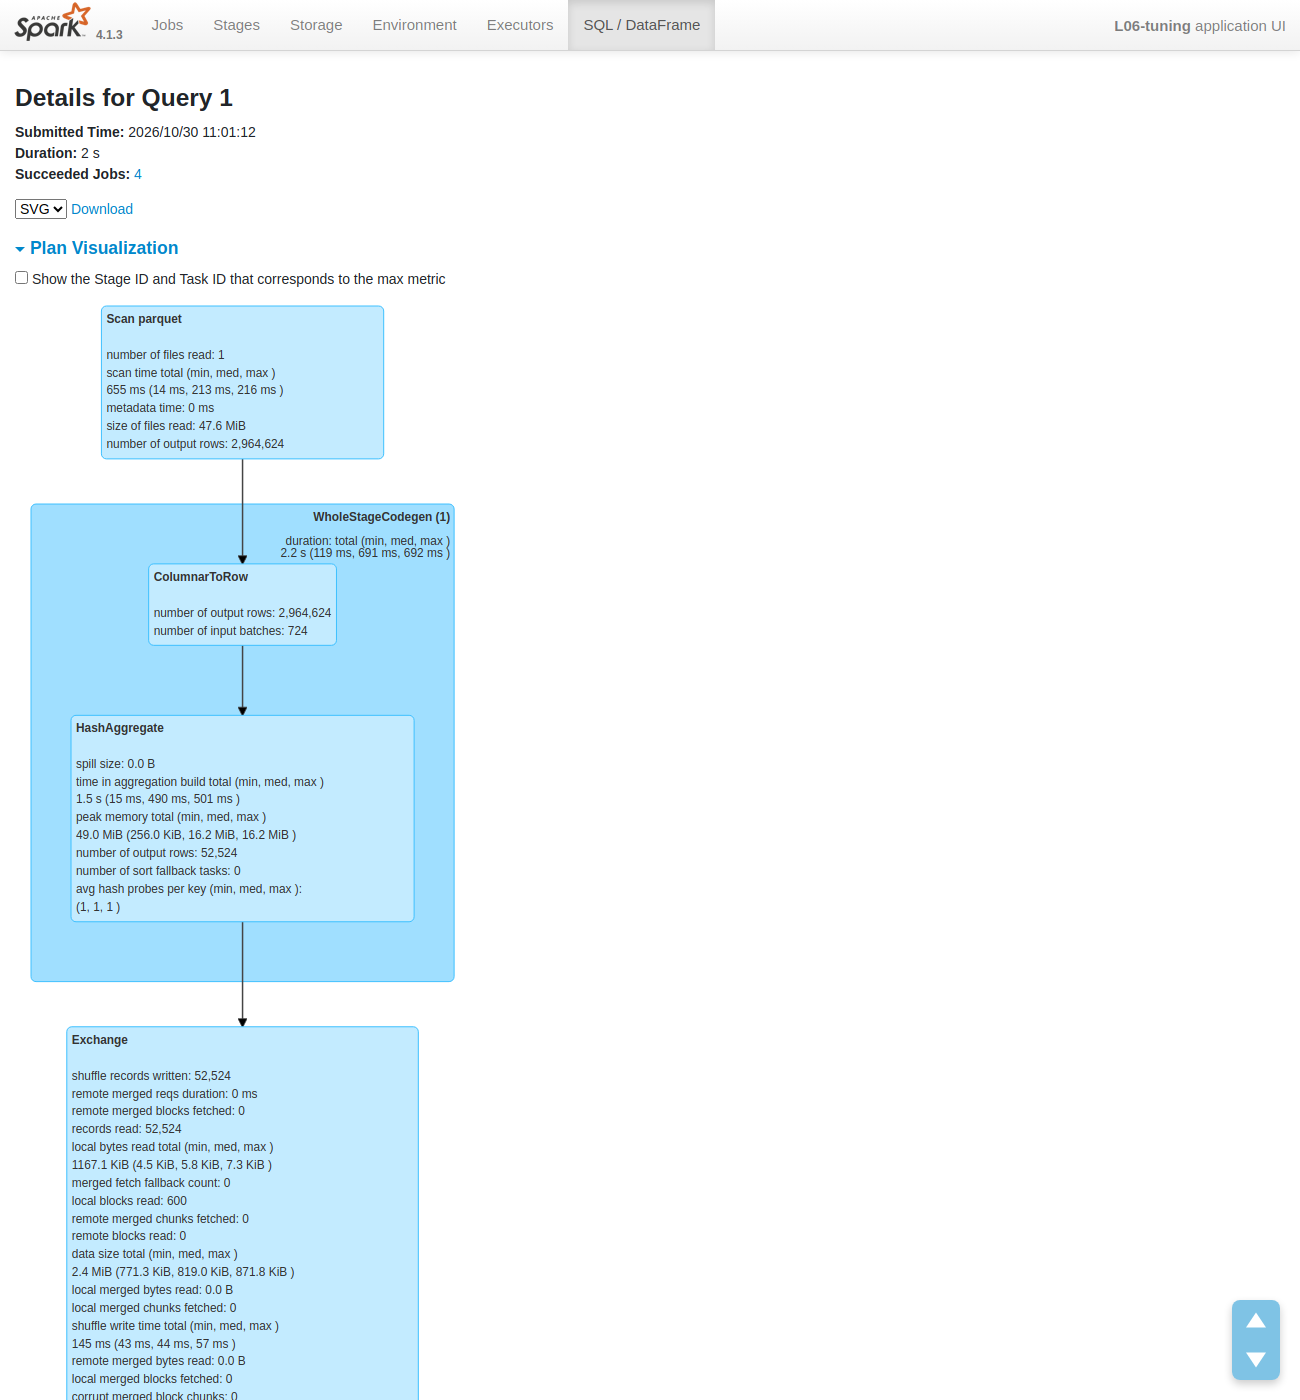
\includegraphics[keepaspectratio]{L06/img/21_ui_e1_aqe_off_200.png}}
\caption{\textbf{E1}: AQE off, 200 partition → \texttt{Exchange} 200
partition}
\end{figure}

\begin{figure}
\centering
\pandocbounded{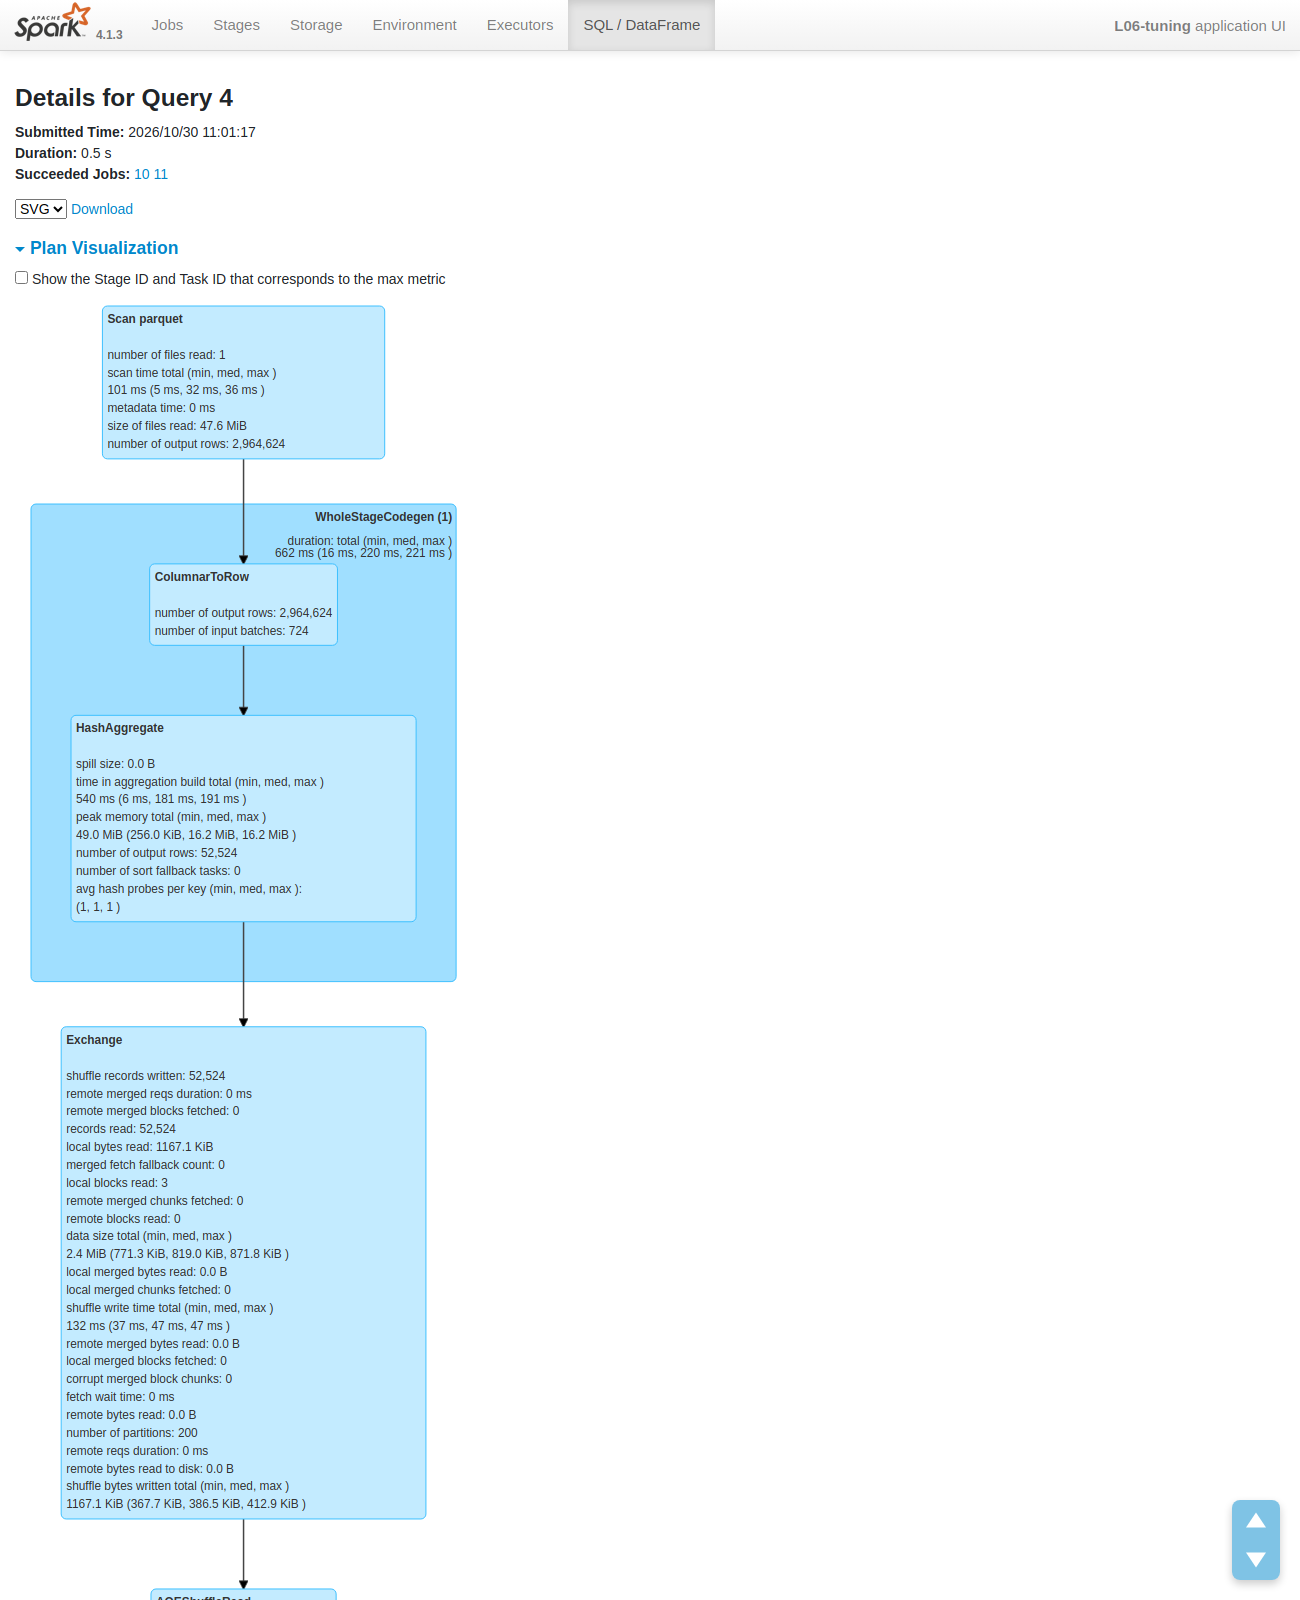
\includegraphics[keepaspectratio]{L06/img/22_ui_e1_aqe_on_coalesced.png}}
\caption{\textbf{E1}: AQE on → \texttt{AQEShuffleRead} \emph{coalesced}}
\end{figure}

\begin{figure}
\centering
\pandocbounded{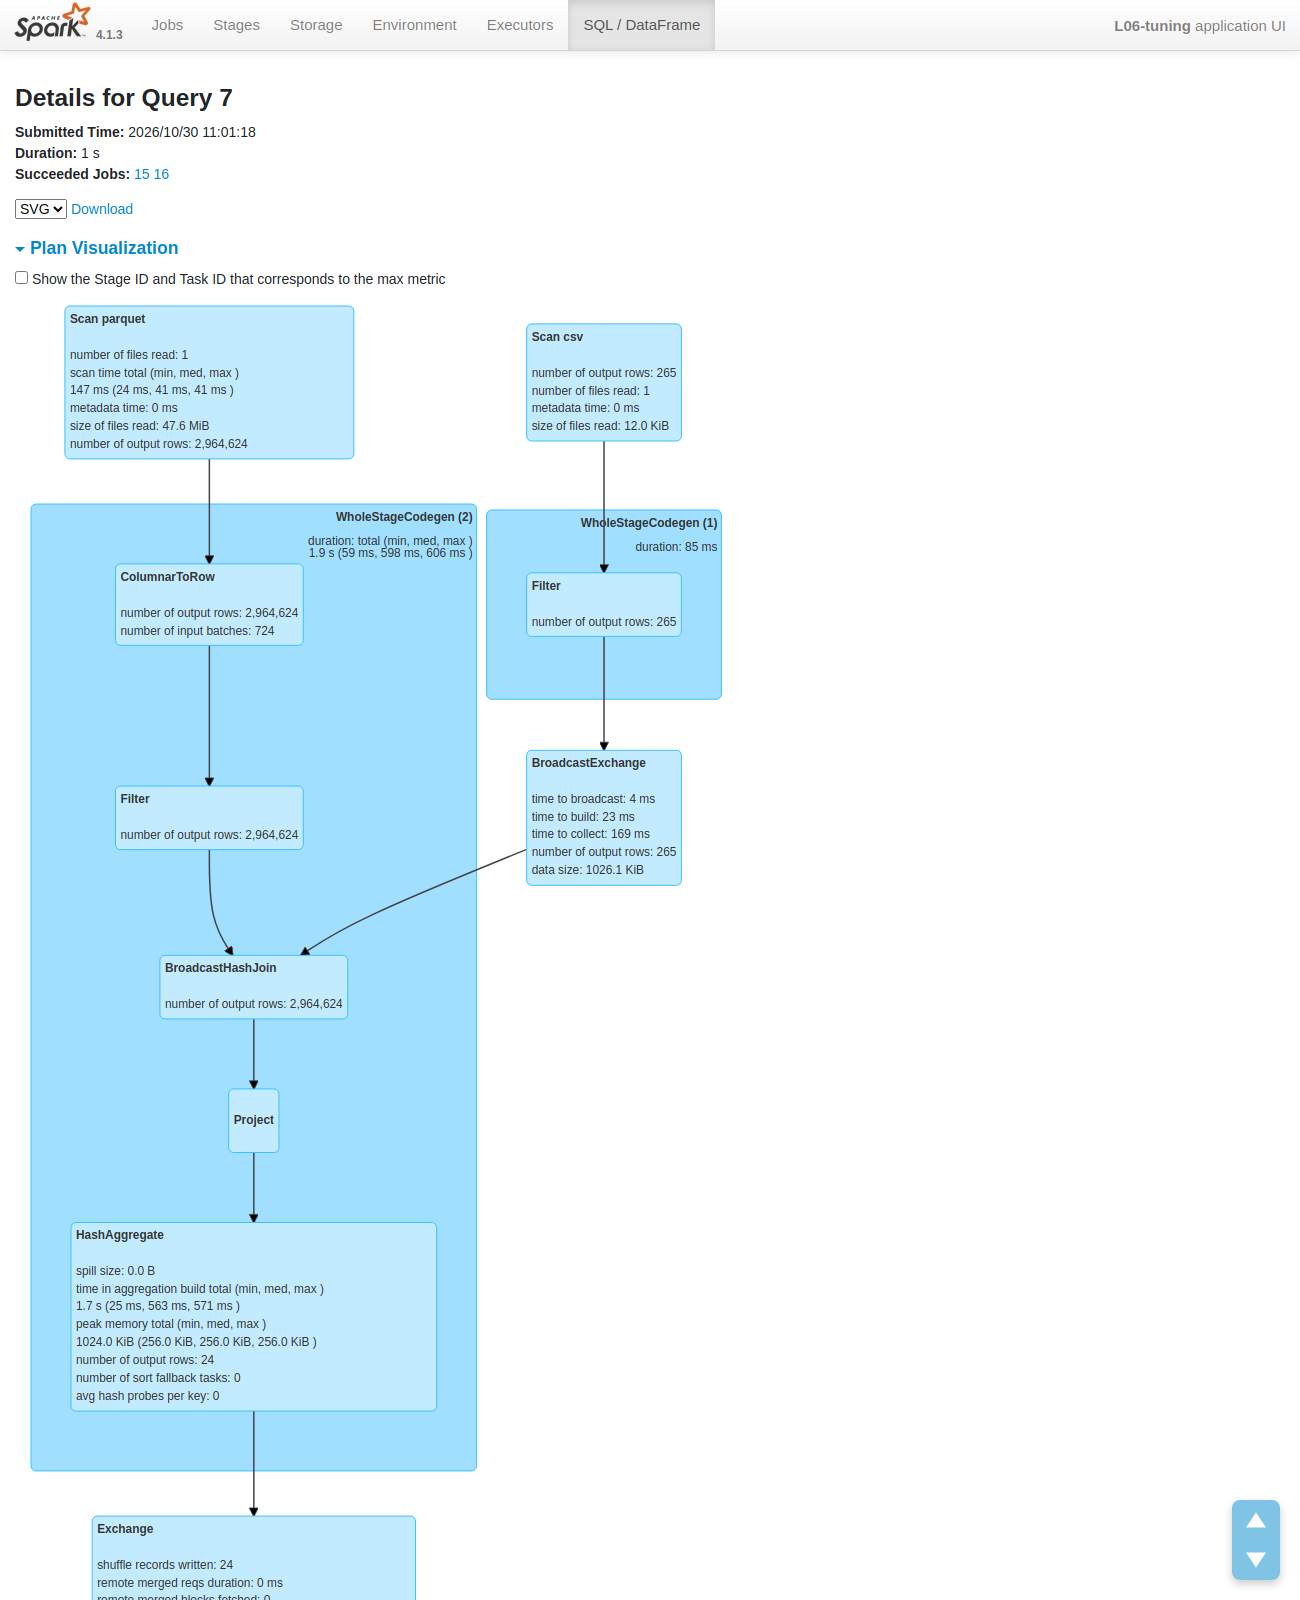
\includegraphics[keepaspectratio]{L06/img/23_ui_e2_broadcast.png}}
\caption{\textbf{E2}: \texttt{BroadcastExchange} +
\texttt{BroadcastHashJoin}}
\end{figure}

\begin{figure}
\centering
\pandocbounded{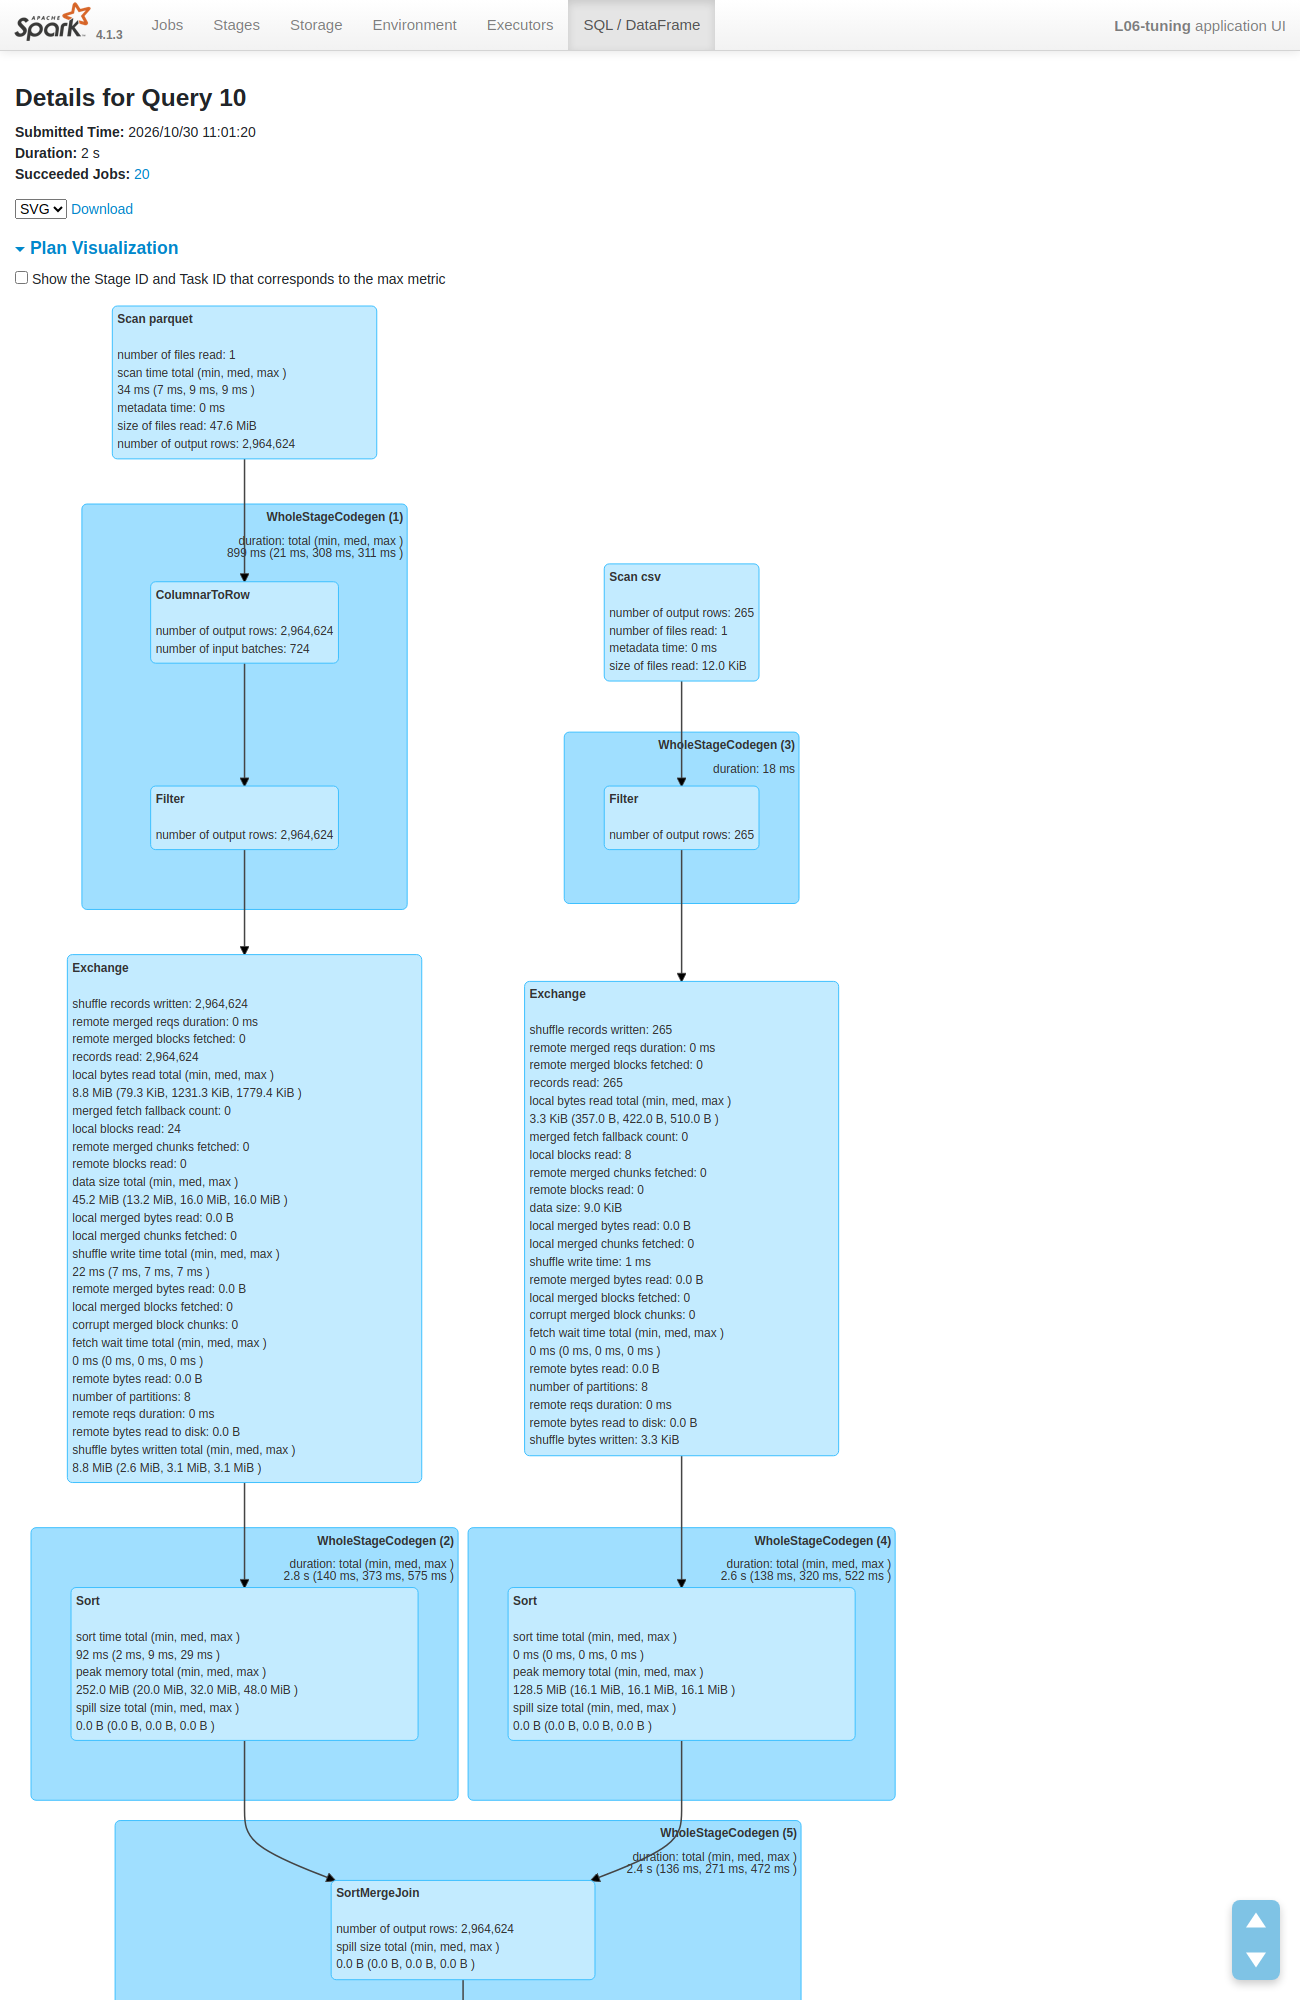
\includegraphics[keepaspectratio]{L06/img/24_ui_e2_sortmerge.png}}
\caption{\textbf{E2}: threshold -1 → \texttt{Exchange} + \texttt{Sort}
hai phía + \texttt{SortMergeJoin}}
\end{figure}

\begin{figure}
\centering
\pandocbounded{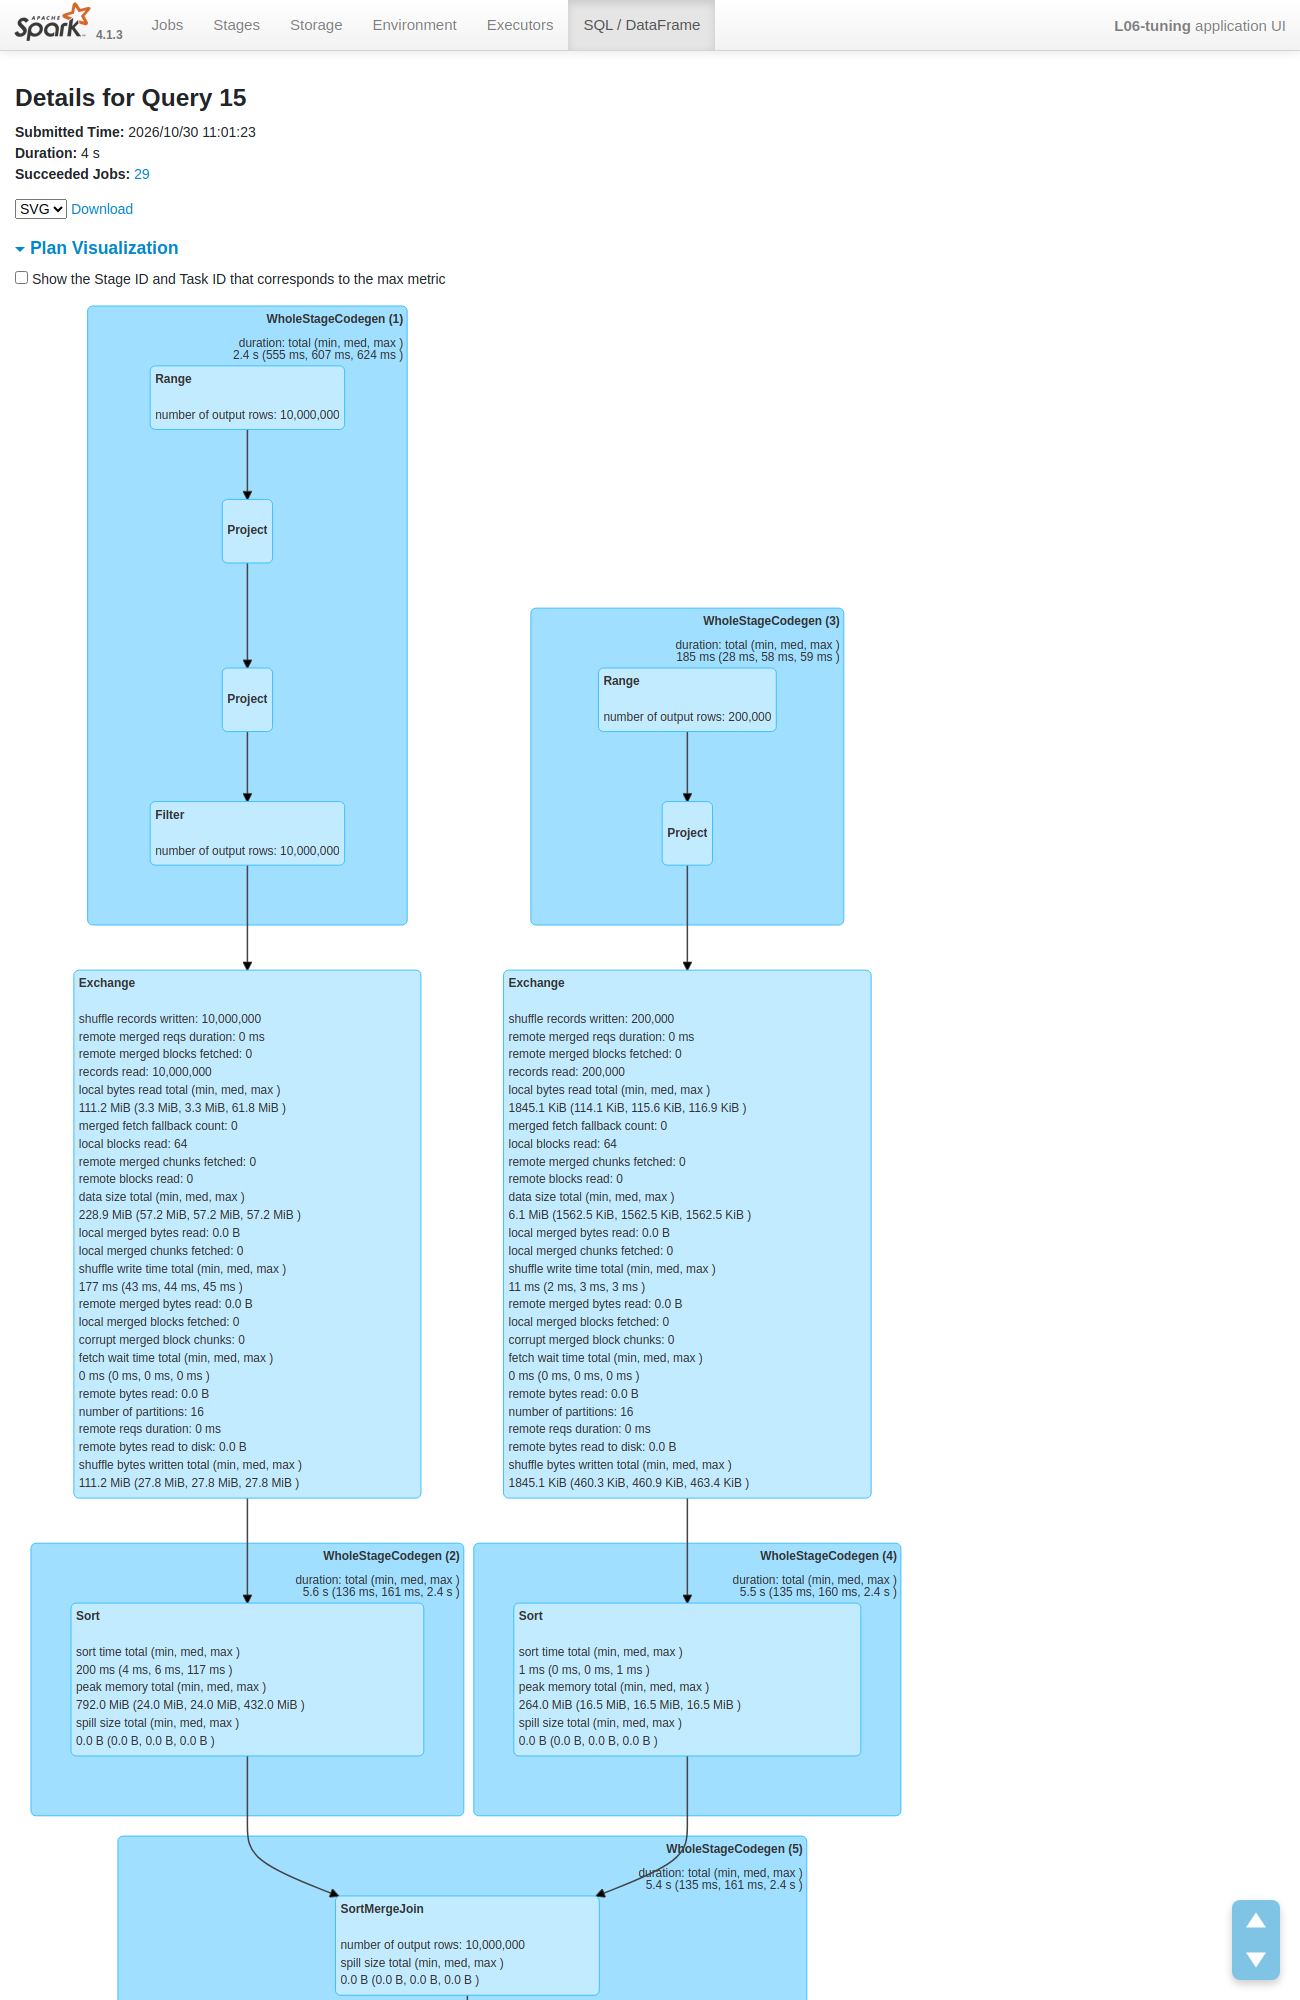
\includegraphics[keepaspectratio]{L06/img/25_ui_e3_skew_baseline_smj.png}}
\caption{\textbf{E3}: baseline SMJ}
\end{figure}

\begin{figure}
\centering
\pandocbounded{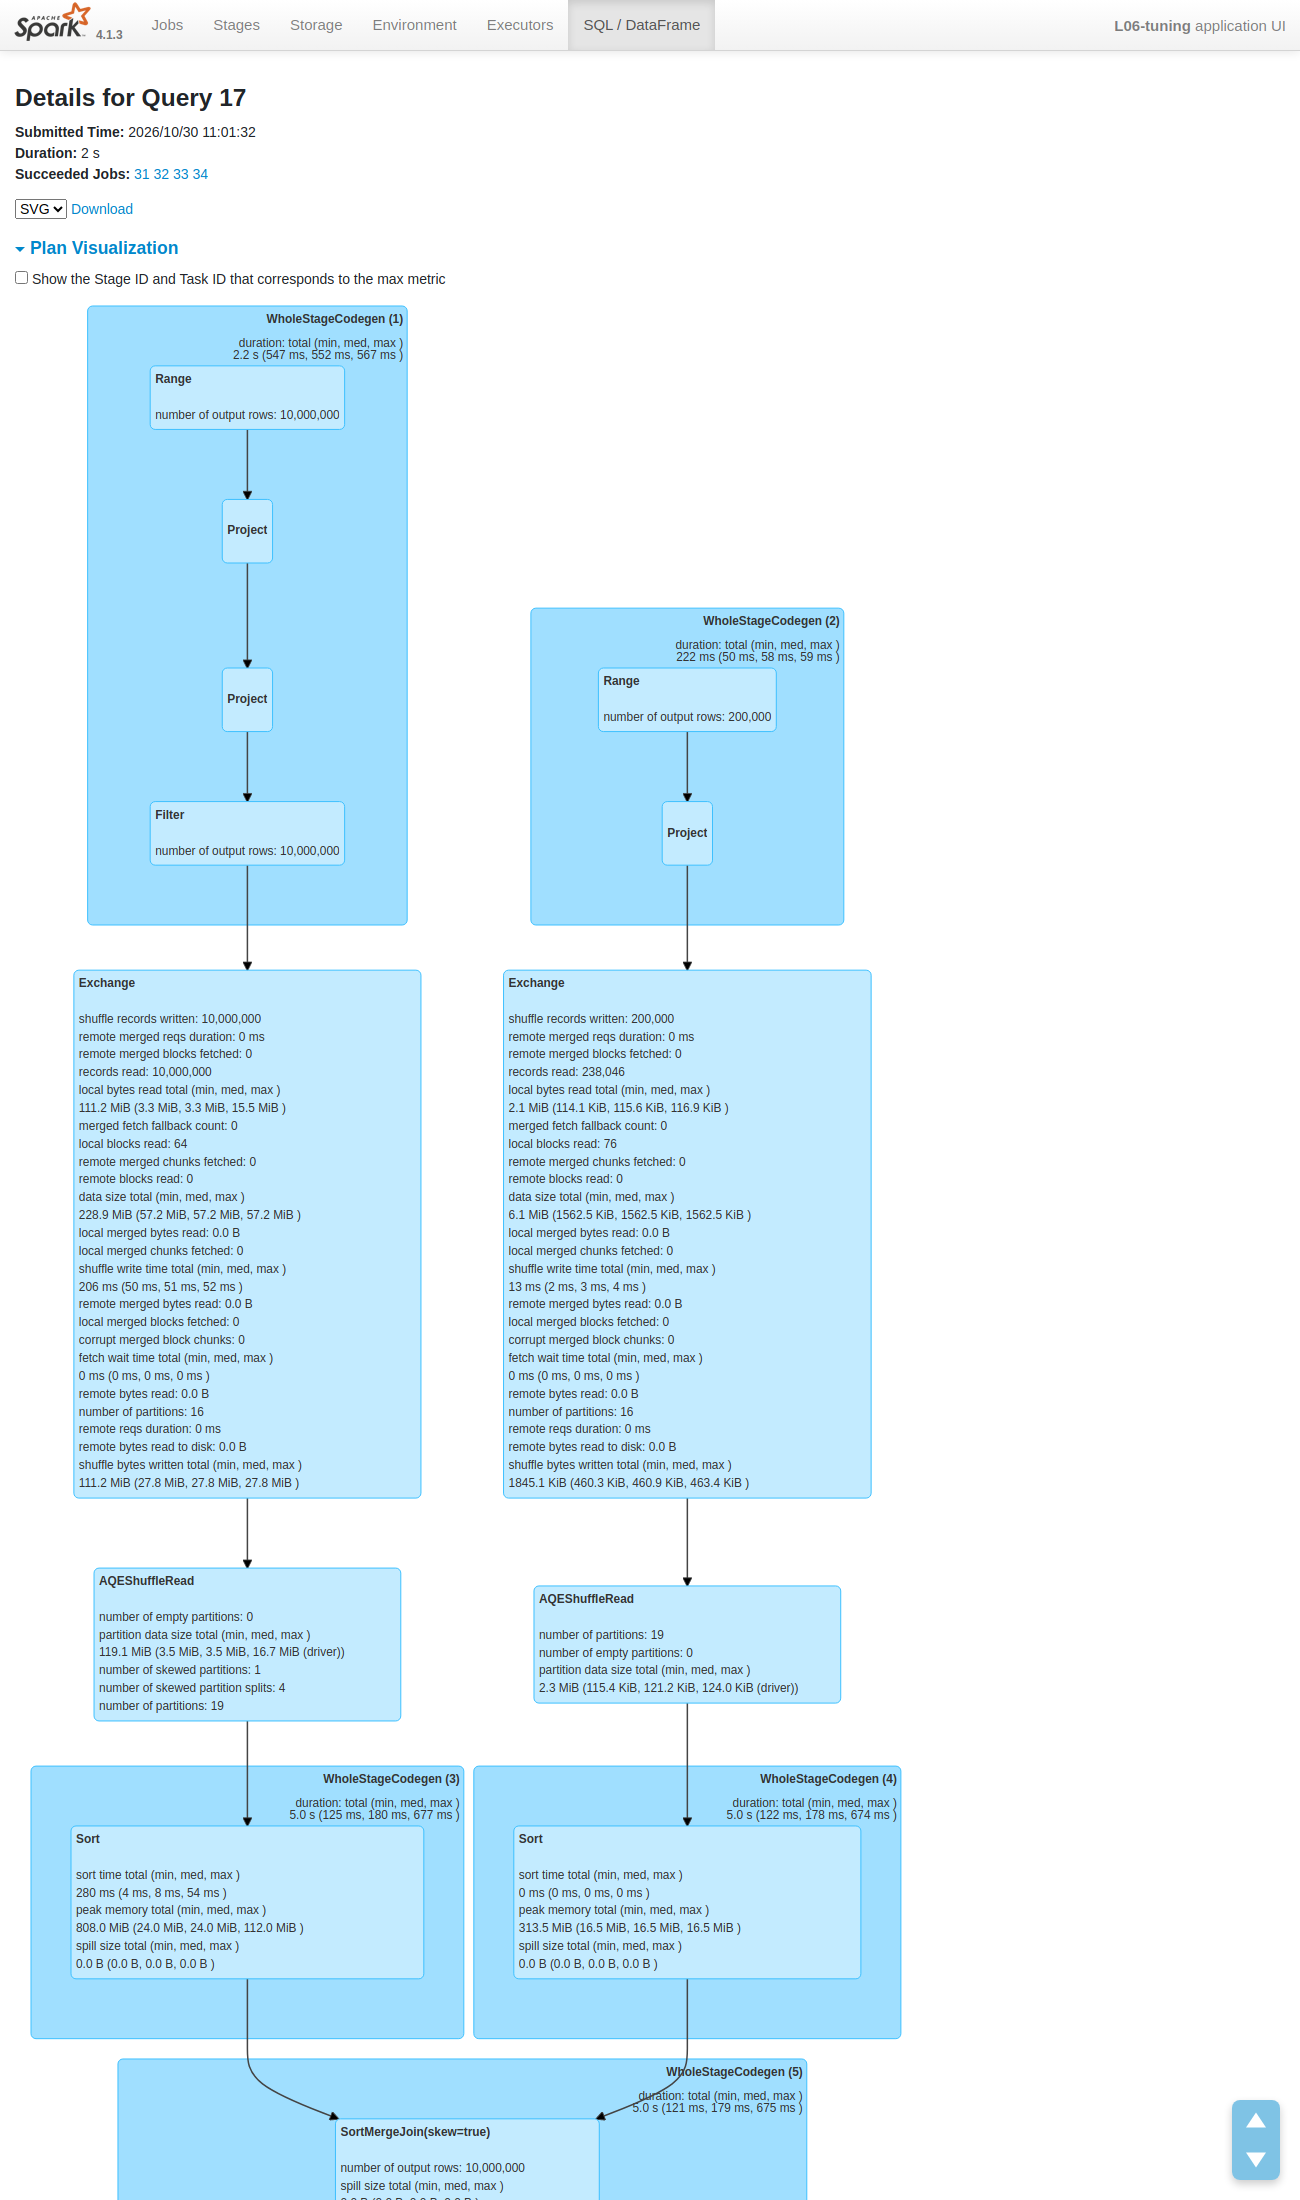
\includegraphics[keepaspectratio]{L06/img/26_ui_e3_aqe_skew_join.png}}
\caption{\textbf{E3}: AQE → \texttt{AQEShuffleRead} (\emph{skewed
partitions: 1, splits: 4, partitions: 19}) +
\texttt{SortMergeJoin(skew=true)}}
\end{figure}

\begin{figure}
\centering
\pandocbounded{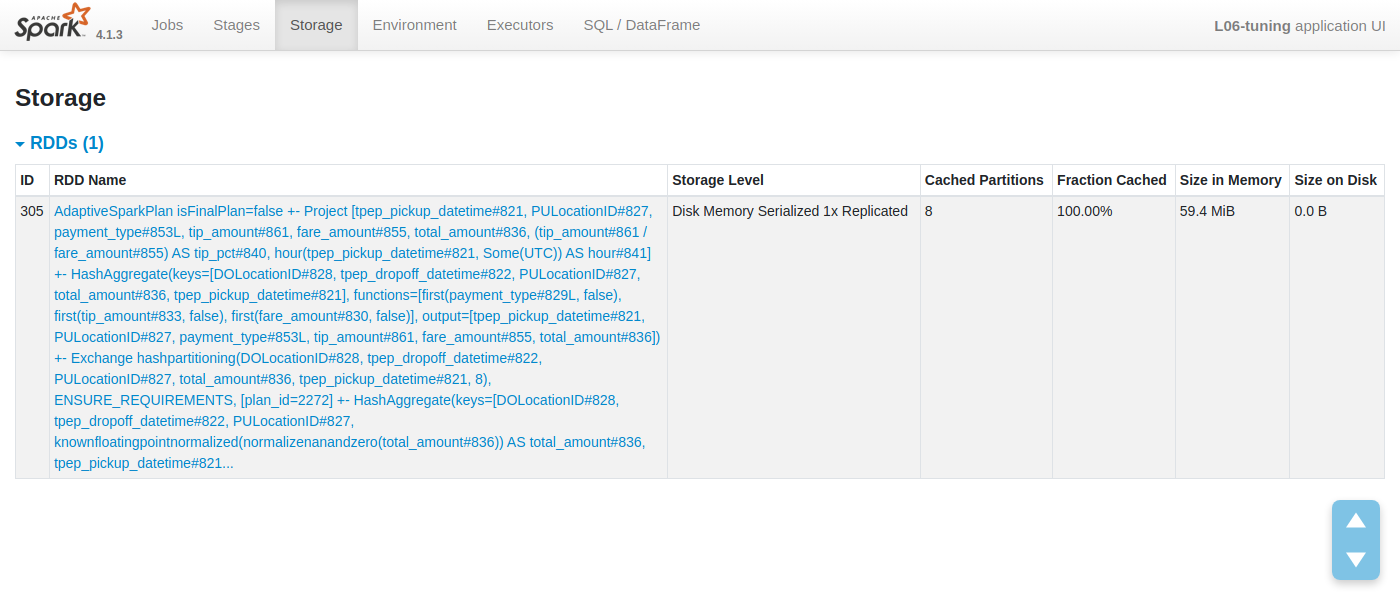
\includegraphics[keepaspectratio]{L06/img/27_ui_storage_e5_cache.png}}
\caption{\textbf{E5}: Storage tab, \texttt{cleaned} cache 8/8 partition,
100 \%, 59.4 MiB}
\end{figure}

\begin{figure}
\centering
\pandocbounded{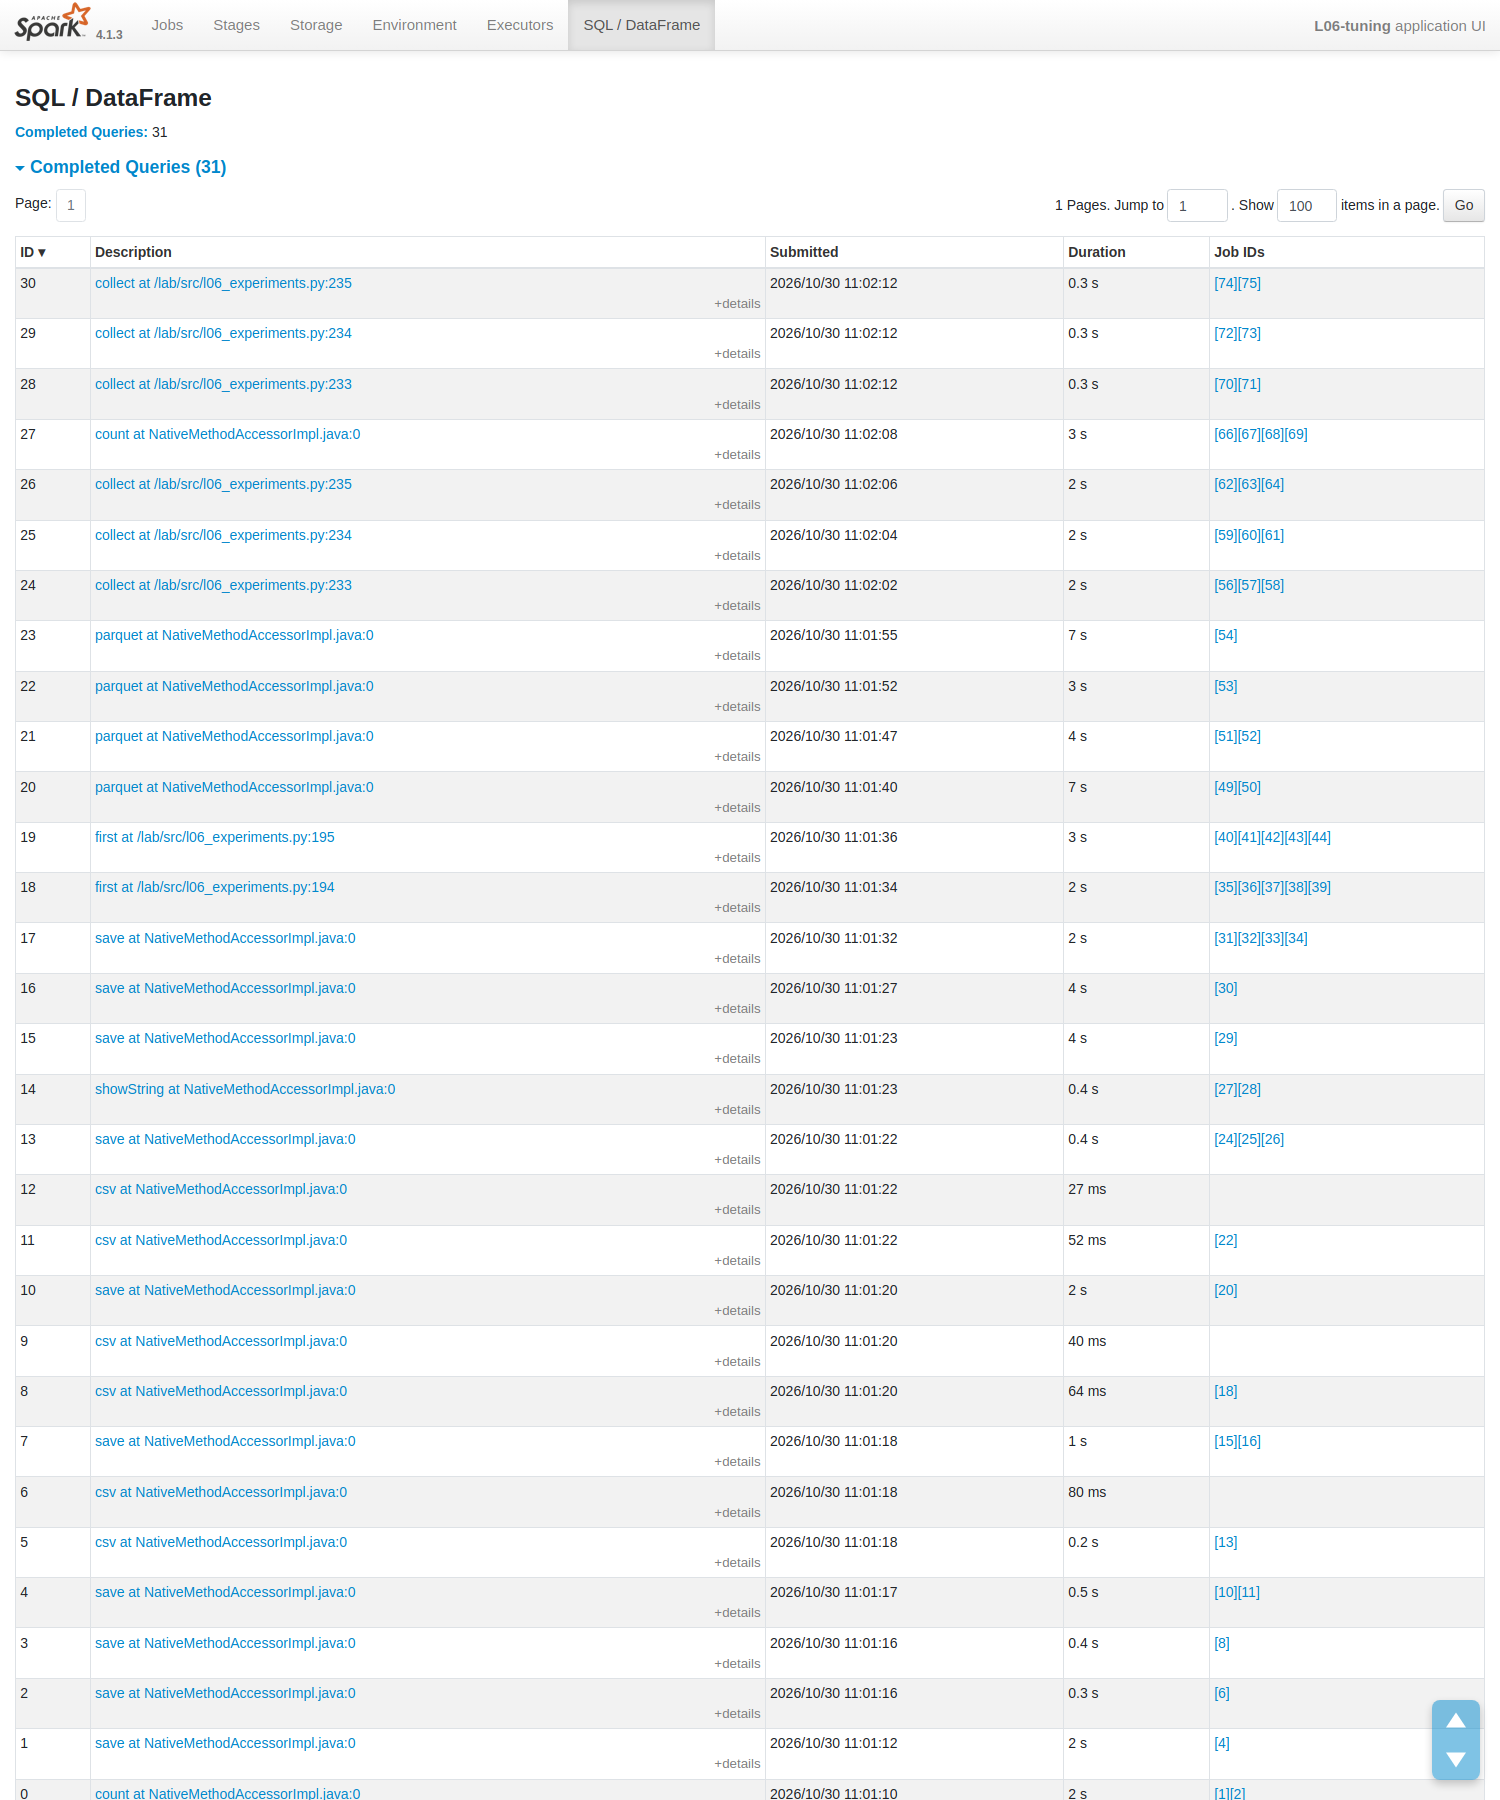
\includegraphics[keepaspectratio]{L06/img/20_ui_sql_list.png}}
\caption{Danh sách SQL query}
\end{figure}

\subsubsection{Skew: Summary Metrics của stage
join}\label{skew-summary-metrics-cux1ee7a-stage-join}

\begin{longtable}[]{@{}
  >{\raggedright\arraybackslash}p{(\linewidth - 4\tabcolsep) * \real{0.3333}}
  >{\raggedright\arraybackslash}p{(\linewidth - 4\tabcolsep) * \real{0.3333}}
  >{\raggedright\arraybackslash}p{(\linewidth - 4\tabcolsep) * \real{0.3333}}@{}}
\toprule\noalign{}
\begin{minipage}[b]{\linewidth}\raggedright
Stage
\end{minipage} & \begin{minipage}[b]{\linewidth}\raggedright
Task time min / median / max
\end{minipage} & \begin{minipage}[b]{\linewidth}\raggedright
Shuffle records median / max
\end{minipage} \\
\midrule\noalign{}
\endhead
\bottomrule\noalign{}
\endlastfoot
42: baseline, AQE off & 140 / 165 / \textbf{2,366 ms} & 262,619 /
\textbf{6,264,438} (61.9 MiB, so với 3.4 MiB) \\
46: salting 64 & 308 / 590 / 1,197 ms & 638,133 / 917,267 \\
52: AQE skew join & 129 / 186 / 682 ms & 262,677 / 1,576,365 (≈ 6.26 M /
4) \\
\end{longtable}

\pandocbounded{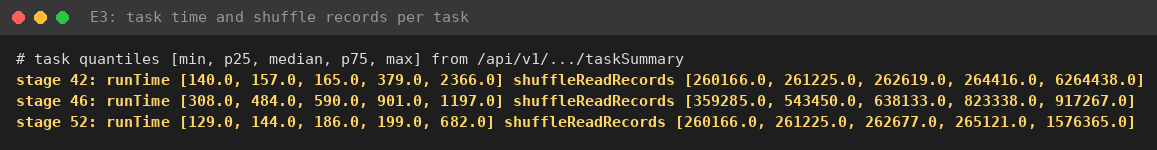
\includegraphics[keepaspectratio]{L06/img/03_e3_task_quantiles.png}}
\pandocbounded{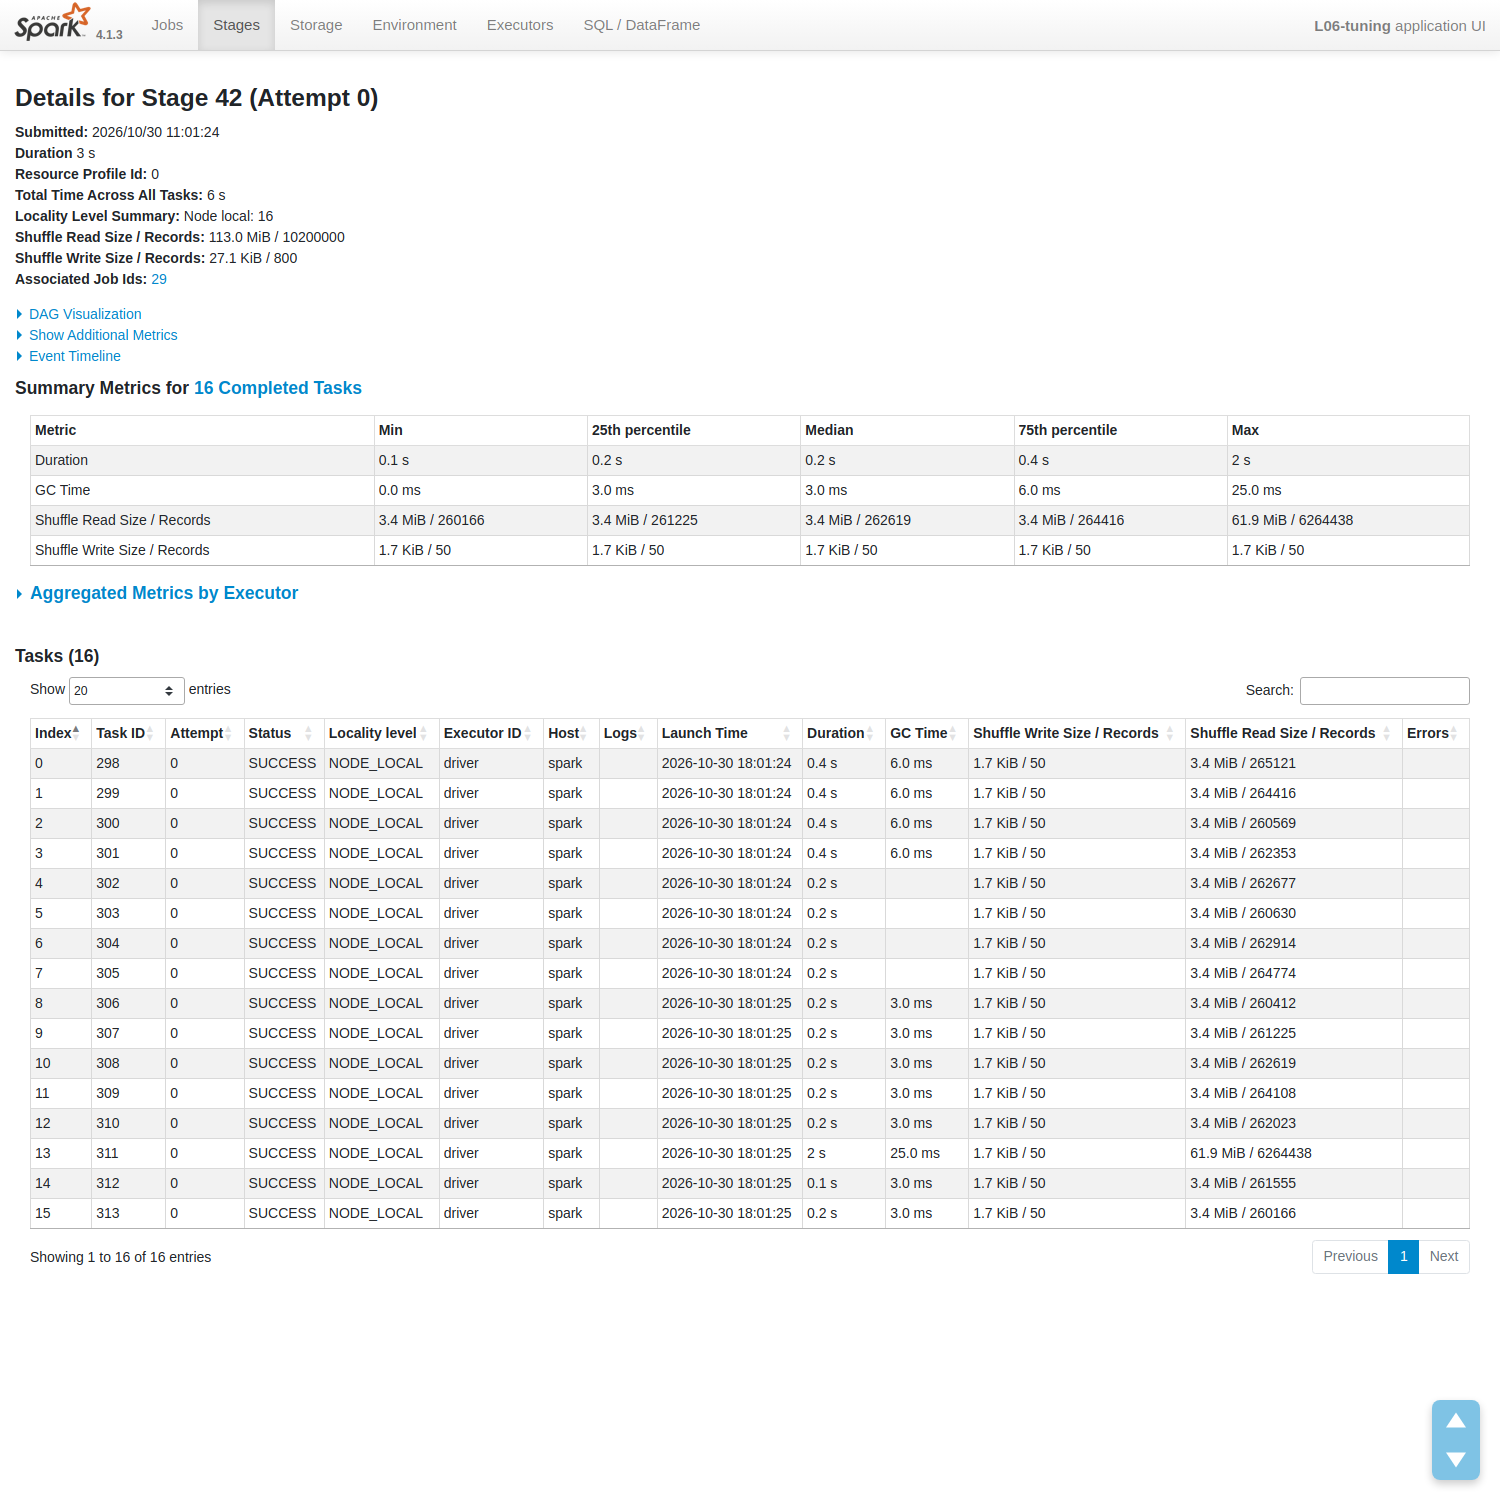
\includegraphics[keepaspectratio]{L06/img/30_ui_e3_baseline_stage42_summary.png}}
\pandocbounded{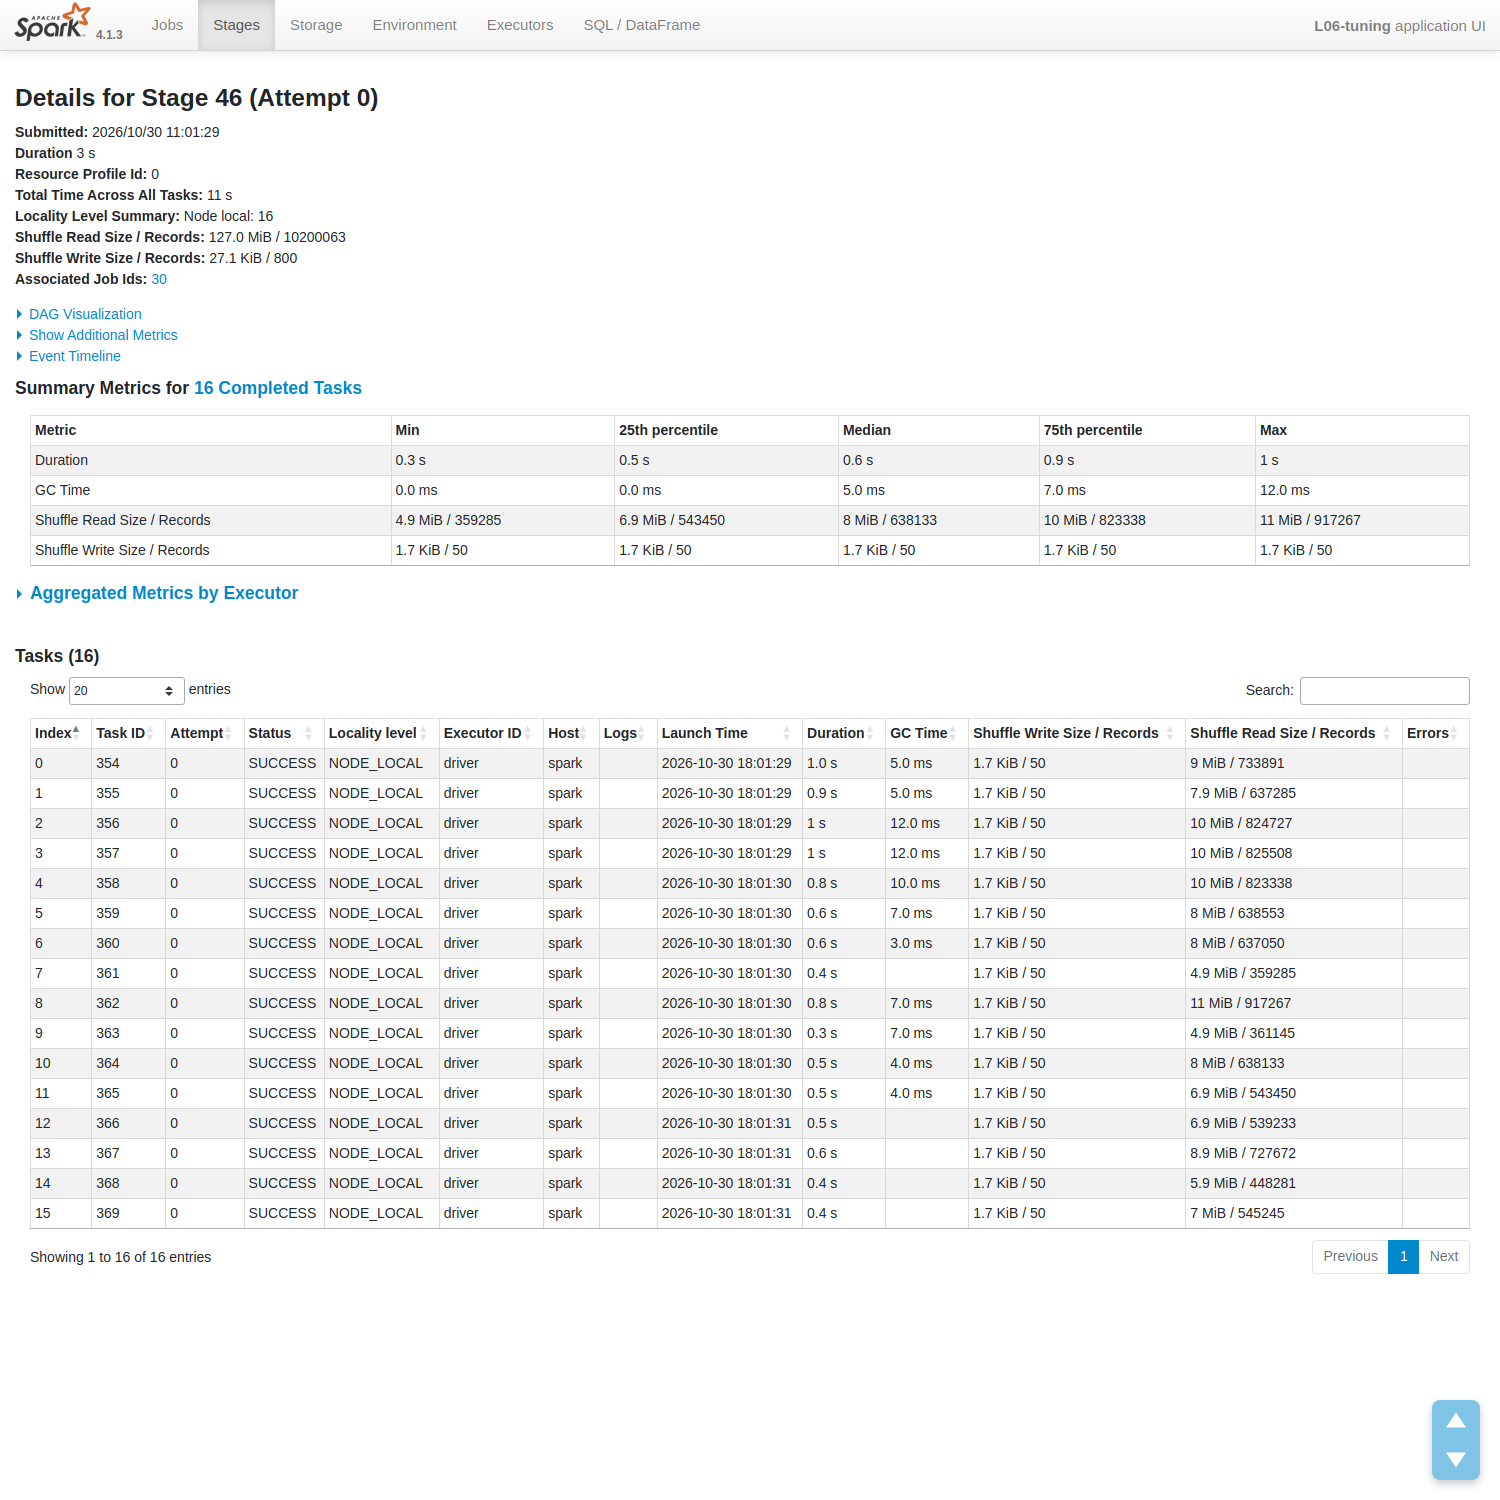
\includegraphics[keepaspectratio]{L06/img/31_ui_e3_salted_stage46_summary.png}}
\pandocbounded{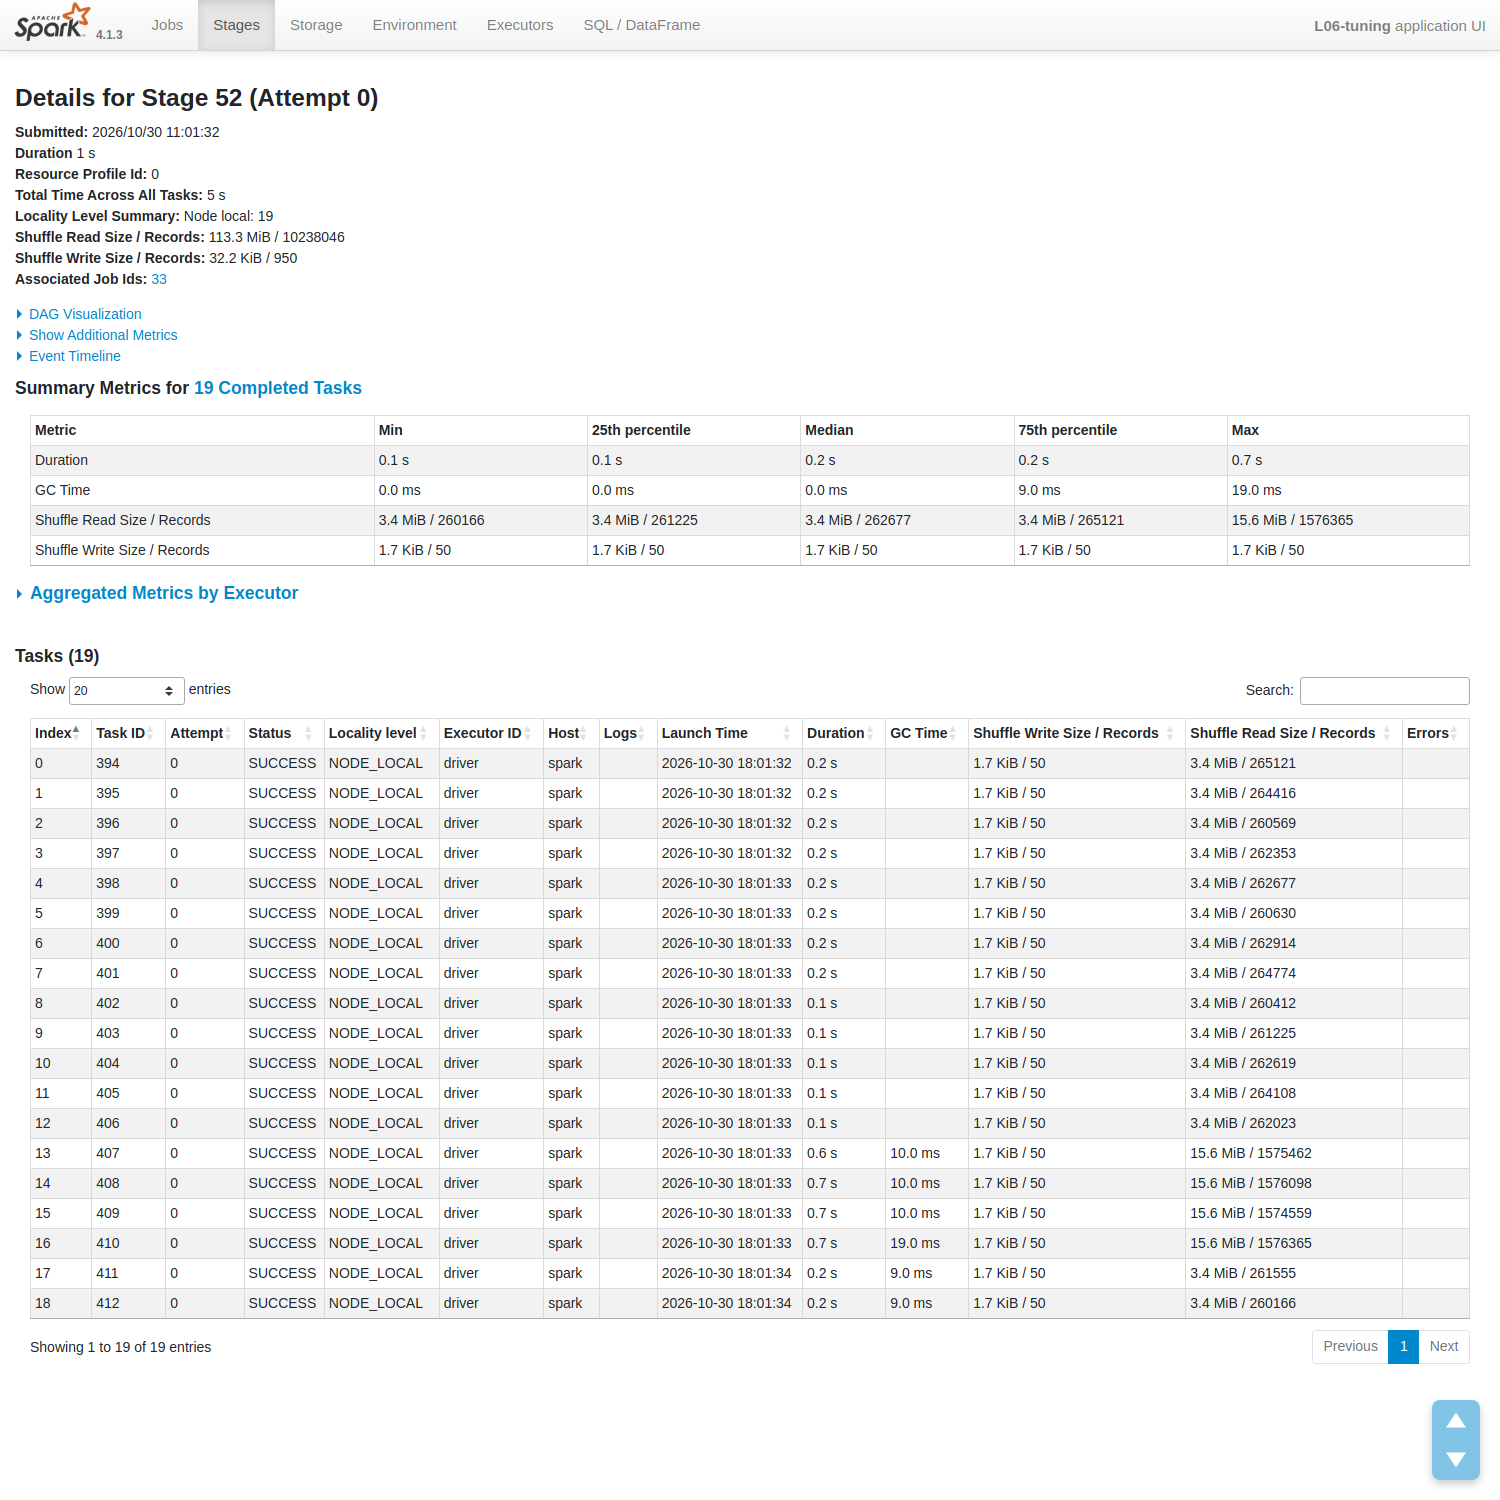
\includegraphics[keepaspectratio]{L06/img/32_ui_e3_aqe_stage52_summary.png}}

\subsection{Trả lời checkpoint}\label{trux1ea3-lux1eddi-checkpoint-5}

\textbf{Q1.} Kết quả \texttt{groupBy(PU,\ DO)} chỉ có vài MB, khoảng 20
nghìn nhóm. 200 partition nghĩa là 204 task, mỗi task chạy 6 ms; chi phí
lập lịch, serialize và khởi tạo task áp đảo, nên mất 2.2 s so với 0.33 s
khi dùng 8 partition. \texttt{shuffle.partitions=1} nhanh ở đây chỉ vì
dữ liệu shuffle tí hon. Trên dữ liệu thật, một reducer phải xử lý
\textbf{toàn bộ} shuffle: không có song song, spill ra đĩa, dễ OOM. Quy
tắc: khoảng 100--200 MB mỗi partition shuffle, hoặc để AQE tự quyết.

\textbf{Q2.} Sau khi stage map của shuffle chạy xong, AQE có
\textbf{thống kê thật} về kích thước từng partition shuffle (map output
statistics). \texttt{AQEShuffleRead\ coalesced} cho một reducer đọc gộp
nhiều partition nhỏ liền kề cho tới khi đạt
\texttt{advisoryPartitionSizeInBytes}. Nhờ đó 200 partition chỉ còn 1
task reduce (tổng 5 task, thay vì 204). Planner tĩnh chỉ có \textbf{ước
lượng} (kích thước file), và ước lượng thường sai sau filter, join hay
aggregate.

\textbf{Q3.} Con số chứng minh skew là \textbf{task max \(\gg\) median}
ở stage join: 2,366 ms so với 165 ms (khoảng 14×). Task đó đọc 6.26
triệu bản ghi trong khi median chỉ 262 nghìn. Salting giảm straggler
(max 1,197 ms) nhưng \textbf{wall-clock gần như không đổi} (4.10 → 4.01
s). Lý do: - Nó thêm việc ở mọi nơi: \texttt{rand()} cho mỗi dòng, thêm
cột join, 64 bản sao dim. - 6 triệu dòng hot vẫn phải chia trên 16
partition × 4 core, nên median tăng từ 165 lên 590 ms. Với 4 core, tổng
công việc là như nhau, chỉ phân bổ lại.

Salting thắng rõ khi có \textbf{nhiều core và partition}: straggler sẽ
giữ hàng trăm executor ngồi chờ. Nó cũng thắng khi công việc trên mỗi
dòng nặng (dòng rộng, join many-to-many, spill), hoặc khi skew nặng hơn
(ví dụ 90 \% hot).

\textbf{Q4.} Một partition bị coi là skew khi kích thước của nó
\textbf{lớn hơn \texttt{skewedPartitionFactor} × median} \textbf{và} lớn
hơn \texttt{skewedPartitionThresholdInBytes}. - Mặc định là 5× và 256
MB; lab hạ xuống 3× và 16 MB. - Ở đây partition hot 61.9 MiB so với
median 3.4 MiB.

AQE \textbf{tách} partition đó thành nhiều task theo khoảng map output
(ở đây 4 split, nên 16 → 19 partition), rồi \textbf{nhân bản} partition
tương ứng của phía bên kia. Plan khi đó hiện
\texttt{SortMergeJoin(skew=true)}.

Giới hạn của AQE so với salting: - chỉ áp dụng cho join có shuffle ở cả
hai phía (SMJ hoặc shuffled hash); - không áp dụng cho mọi kiểu join
(không tách được phía cần giữ nguyên của outer join); - cần ngưỡng hợp
với dữ liệu; - \textbf{không xử lý skew trong \texttt{groupBy}} hay skew
sau join. Salting, hay aggregate hai pha, xử lý được những trường hợp
này.

\textbf{Q5.} Không nên broadcast dù một bên ``nhỏ'' khi: - bảng đó vẫn
lớn trong bộ nhớ: driver phải collect trước rồi gửi bản sao tới mọi
executor, gây OOM driver hoặc broadcast timeout; - thống kê \textbf{đánh
giá thấp} kích thước, ví dụ sau filter hay UDF; - là \textbf{full outer
join} (không hỗ trợ), hoặc phía cần broadcast là phía được giữ của outer
join; - join chạy lặp lại nhiều lần trên dữ liệu thay đổi, nên mỗi lần
phải dựng lại broadcast.

\textbf{Q6.} - \texttt{repartition(n)} \textbf{luôn shuffle}: partition
cân bằng (4 file đều nhau), và stage trước giữ nguyên song song. Cái giá
là thêm một shuffle (4.40 s). - \texttt{coalesce(n)} gộp partition sẵn
có \textbf{không shuffle}: rẻ (3.12 s), nhưng \textbf{có thể tạo file
lệch}. Ở đây chỉ ra 3 file vì input chỉ có 3 row group, nên một
partition rỗng. - Vì \texttt{coalesce} là narrow dependency, nó
\textbf{giảm song song của cả stage trước}: \texttt{coalesce(1)} chạy
scan và ghi trong \textbf{1 task} (6,800 ms).

\textbf{Q7.} DataFrame được cache là kết quả của một bước \textbf{đắt}
(\texttt{dropDuplicates}, shuffle toàn bộ khoảng 3 triệu dòng) và được
dùng lại 3 lần. - Không cache: dedup chạy 3 lần, 6.40 s. - Có cache:
dedup chạy 1 lần (3.42 s) rồi 3 query chỉ còn 0.99 s.

Một scan Parquet thuần, đã prune cột, thì vốn rẻ: đọc vectorized, có
column pruning và predicate pushdown. Cache khi đó chỉ tốn bộ nhớ và
thời gian materialize, gần như không lợi. Quy tắc: cache cái \textbf{đắt
và được dùng lại}, rồi \texttt{unpersist()}.

\textbf{Q8.} Checklist trước khi mua thêm phần cứng: 1. \textbf{Đọc plan
và Spark UI}: tìm stage chậm nhất, spill, GC, và tỉ lệ task max/median
để phát hiện skew. 2. \textbf{Lọc và chọn cột sớm}: partition pruning,
predicate/column pushdown, dùng định dạng cột (Parquet/ORC). 3.
\textbf{Kích thước partition shuffle hợp lý}: bật AQE (coalesce và skew
join), khoảng 100--200 MB mỗi partition. 4. \textbf{Chọn đúng chiến lược
join}: broadcast bảng nhỏ; với skew thì dùng AQE skew join, salting,
hoặc tách hot key. 5. \textbf{Tránh UDF Python} (dùng hàm built-in hoặc
pandas UDF), \textbf{cache có chọn lọc}, và \textbf{tránh file nhỏ} khi
ghi (repartition hoặc compaction).

\newpage

\end{document}
